%%%%%%%%%%%%%%%%%%%%%%%%%%%%%%%%%%%%%%%%%%%%%%%%%%%%%%%%%%%%%%%%%%%%%%%%%%%%%%%
% CONTRIBUTION TO THE SURFEX BOOK1: "Surface Processes Scheme"
% Author        : P. Le Moigne
% Original      : January 05, 2009
% Last Update   : January 05, 2009
% Last Update   : January 25, 2016 A. Boone, B. Decharme
%%%%%%%%%%%%%%%%%%%%%%%%%%%%%%%%%%%%%%%%%%%%%%%%%%%%%%%%%%%%%%%%%%%%%%%%%%%%%%%

\chapter{Soil and vegetation}
\minitoc
%=========================
\bibliographystyle{plain}
%=========================

%=========================================================================================================
%=========================================================================================================
%=========================================================================================================
\section{ISBA surface scheme}
%=========================================================================================================
%=========================================================================================================
%=========================================================================================================


%=========================================================================================================
%=========================================================================================================
\subsection{Surface snow fractions}
%=========================================================================================================
%=========================================================================================================

Snow is known to have a significant impact on heat conduction fluxes owing to it’s relatively high
insulating properties. In addition, it can significantly reduce turbulent transfer owing to reduced
surface roughness, and it has a relatively large surface albedo
thereby impacting the surface net radiation budget. Thus, for
spatially distributed (parcel, meso, regional and/or global scales), 
the parameterization of it’s areal coverage turns out to be a critical
aspect of land surface model (LSM) representation
of snowpack-atmosphere interactions and sub-surface soil and
hydrological processes.
%
For example, the areal snow cover fraction for each patch
of the ISBA land surface model has an impact
on the total upwelling radiative and turbulent fluxes, in addition to
soil freezing (depth and intensity), and snow melt rates. 
%
In ISBA (like many other land surface models), the total snow fraction
for a given surface is comprised of several component fractions which
are described herein.

First, the snow fraction over vegetation is computed from
%
%%%%%%%%%%%%%%%%%%%%%%%%%%%%%%%%%%%%%%%%%%%%%%%%%
\begin{equation}
\label{eq:isba_snow_frac_veg}
p_{snv} \,\, =\,\,  \frac{ h_s }{ h_s + w_{sv} \, z_0 } 
\end{equation}
%%%%%%%%%%%%%%%%%%%%%%%%%%%%%%%%%%%%%%%%%%%%%%%%%
%
where $z_0$ is the surface roughness length (including the effects of
snow cover, soil, vegetation...).
$h_s$ (m) is the single-layer total snow 
depth. It is defined as 
%
%%%%%%%%%%%%%%%%%%%%%%%%%%%%%%%%%%%%%%%%%%%%%%%%%
\begin{equation}
%
h_s \,\,=\,\,  W_s / \rho_s
%
\end{equation}
%%%%%%%%%%%%%%%%%%%%%%%%%%%%%%%%%%%%%%%%%%%%%%%%%
%
where $\rho_s$ (kg m$^{-3}$) is the average single-layer
snowpack density and $W_s$ (kg m$^{-2}$) is the single-layer bulk snow water
equivalent (or $SWE$).
The empirical parameter $w_{sv}$ is a coefficient set to 5 (default). 
%
The snow cover fraction for the bareground portion of the patch is
given by
%
%%%%%%%%%%%%%%%%%%%%%%%%%%%%%%%%%%%%%%%%%%%%%%%%%
\begin{equation}
\label{eq:isba_snow_frac_ground}
p_{sng} \,\, = \frac{W_s}{\left(W_s + W_{crn}\right)}
%
\end{equation}
%%%%%%%%%%%%%%%%%%%%%%%%%%%%%%%%%%%%%%%%%%%%%%%%%
%
The critical snow water equivalent is defined as
$W_{crn} = 10$ kg m$^{-2}$.

Note that the formulation for $p_{sng}$ is slightly different for the
multi-layer snow schemes.
In this case, it is defined as
%
%%%%%%%%%%%%%%%%%%%%%%%%%%%%%%%%%%%%%%%%%%%%%%%%%
\begin{equation}
\label{eq:isba_snow_frac_ground_explicit}
p_{sng} = {\rm min} \left(1,\, D_n/D_{ng} \right) 
\end{equation}
%%%%%%%%%%%%%%%%%%%%%%%%%%%%%%%%%%%%%%%%%%%%%%%%%
%
where $D_n$ is the total depth for a multi-layer snow scheme option and
$D_{ng}$ (m) a ground snow depth threshold set to 0.01 m.
Note that $D_n$ is analogous to $h_s$, but different symbols are used
to distinguish between the single-layer snow-scheme bulk depth, $h_s$, and the
total depth, $D_n$, as a sum of multiple layer thicknesses for the
multi-layer snow scheme options.

The total snow cover fraction, $p_{sn}$ 
is computed as the sum between the bare
ground snow covered fraction, $p_{sng}$, and the fraction of vegetation
covered by snow, $p_{snv}$, weighted by the vegetation fraction of the
patches covered by vegetation, $veg$ as
%
%%%%%%%%%%%%%%%%%%%%%%%%%%%%%%%%%%%%%%%%%%%%%%%%%
\begin{equation}
\label{eq:isba_snow_frac_total}
p_{sn} = (1-veg) p_{sng} + veg \, p_{snv}
%
\end{equation}
%%%%%%%%%%%%%%%%%%%%%%%%%%%%%%%%%%%%%%%%%%%%%%%%%
%
$veg$ is specified for each
vegetation patch: it is equal to 0.0 for bare soil, 0.95 for
grassland/tundra as well as for temperate and boreal forests, and
varies exponentially according to the leaf area index ($LAI$) for crop
types.
%
As a final note, a recent explicit canopy vegetation (bulk-layer)
option (called the multi-energy budget or ISBA-MEB option)
has been added to ISBA. In this parameterization, 
neither $veg$ or $p_{snv}$ are used 
(thus for MEB, $p_{sn}=p_{sng}$): thus MEB has a much lower
dependence on the empirical snow fraction
parameterization. In addition, vegetation can be buried (for
sufficiently deep snowpacks) in the
vertical sense for MEB: see Section~\ref{sec:isba_meb} for details.

%=========================================================================================================
%=========================================================================================================
\subsection{Force restore approach}
%=========================================================================================================
%=========================================================================================================

%=========================================================================================================
\subsubsection{Treatment of the soil heat content}
%=========================================================================================================

The prognostic equations for the surface temperature
$T_s$ and its mean value $T_2$ over one day $\tau$,
are obtained from the force-restore method proposed by
Bhumralkar (1975)\nocite{Bhumralkar1975} and Blackadar (1976)\nocite{Blackadar1976}:
%
%%%%%%%%%%%%%%%%%%%%%%%%%%%%%%%%%%%%%%%%%%%%%%
\begin{align} 
\label{eqTs}
\frac{\partial T_s}{\partial t} \,\, =& \,\,
C_T (R_n-H-LE) - \frac{2\pi}{\tau} \left(T_s-T_2\right)   
\\
\label{eqT2}
\frac{\partial T_2 }{ \partial t} \,\, =& \,\, \frac{1}{\tau} \left(T_s-T_2\right)
\end{align} 
%%%%%%%%%%%%%%%%%%%%%%%%%%%%%%%%%%%%%%%%%%%%%%
%
where $H$ and
$LE$ are the sensible and latent heat fluxes, and
$R_n$ is the net radiation at the surface.
The surface temperature $T_s$ evolves due to both the
diurnal forcing by the heat flux $G = R_n-H-LE$ and
a restoring term towards its mean value $T_2$.
In contrast, the mean temperature $T_2$ only varies
according to a slower relaxation towards $T_s$.

The coefficient $C_T$ is expressed by
%
\begin{equation}
C_T=1 / \left[  \frac{(1-veg)(1-p_{sng}) }{ C_g}
    +       \frac{ veg(1-p_{snv}) }{ C_v }
    +       \frac{ p_{sn} }{ C_s } \right]
\end{equation}
where $veg$ is the fraction of vegetation, $C_g$ is the ground heat capacity,
$C_s$ is the snow heat capacity, and $C_v$ is the vegetation heat
capacity.
The snow cover fraction for the bare-ground 
portion of the patch is computed from Eq.~\ref{eq:isba_snow_frac_ground}.
%
The partitioning of the grid into bare soil, vegetation, and snow areas,
is indicated in Fig.(\ref{isba1}) .

\begin{figure}[h]
\begin{center}
\psfig{figure=\EPSDIR/isba_fig1.pdf,width=10cm}
\caption{Partitioning of the grid \label{isba1}}
\end{center}
\end{figure}

The heat capacities of the ground and snow canopies are
respectively given by
%
%%%%%%%%%%%%%%%%%%%%%%%%%%%%%%%%%%%%%%%%%%
\begin{equation}
C_g=C_{gsat} \left( w_{sat}/w_2 \right)^
{b / 2{\rm log}10} 
\hskip.5in
\left( C_g \leq 1.5 \times 10^{-5}\right)
\end{equation}
%%%%%%%%%%%%%%%%%%%%%%%%%%%%%%%%%%%%%%%%%%
%
where $G_{gsat}$ (K m$^2$ J$^{-1}$) is the heat capacity at
saturation, 
and $w_{sat}$ the
volumetric moisture content of the soil at saturation; and
%
%%%%%%%%%%%%%%%%%%%%%%%%%%%%%%%%%%%%%%%%%%
\begin{equation}
C_s = 2 \, \left( \frac{\pi }{ \lambda_s c_s \tau}
\right)^{1/2}
\end{equation}
%%%%%%%%%%%%%%%%%%%%%%%%%%%%%%%%%%%%%%%%%%
%
where $\lambda_s = \lambda_i \times {\rho_s}^{1.88}$;
$c_s = c_i (\rho_s / \rho_i)$:
$\lambda_i$ is the ice conductivity;
$c_i$ is the heat capacity
of ice; and $\rho_i$ is the relative density
of ice (Douville, 1994\nocite{Douville1994}; Douville \etal 1995\nocite{Douville1995}).
\\

After an intermediate surface
temperature ${T_s}^*$ is evaluated from Eq. (\ref{eqTs}), the cooling
due to the melting of snow is considered following
\begin{eqnarray}
{T_s}^+ = {T_s}^\ast - C_T \,L_f \,M_{lt}\Delta t
\end{eqnarray}
where $L_f$ is the latent of fusion, $\Delta t$ is the timestep,
and the melting rate of snow is
\begin{eqnarray}
M_{lt} = p_{sn} \left( \frac{ T_n - T_0 }{ C_s L_f \Delta t } \right)
\hskip.5in
\left(M_{lt}\geq 0\right)
\end{eqnarray}
%Here, the reference meting temperature is simply defined
%as the triple point, $T_0=T_f=273.16$ K, and 
%
and
%
%%%%%%%%%%%%%%%%%%%%%%%%%%%%%%%%%%%%%%%%%%
\begin{equation}
%
T_n \, = \, (1-veg) {T_s}^\ast + veg \, T_2
%
\end{equation}
%%%%%%%%%%%%%%%%%%%%%%%%%%%%%%%%%%%%%%%%%%
%
Similarly, the intermediate mean temperature ${T_2}^\ast$ 
is also modified due to the melting/freezing of
water in the soil layer occurring for temperatures
(Boone \etal 2000\nocite{Boone2000}).
The resulting mean temperature is
\begin{eqnarray}
{T_2}^+ = {T_2}^\ast + \left(\Delta w_2\right)_{frozen} L_f \, C_g \, d_f
\end{eqnarray}
with
%
%%%%%%%%%%%%%%%%%%%%%%%%%%%%%%%%%%%%%%%%%%
\begin{equation}
%
(\Delta w_2)_{frozen} \,\, = \,\, \Bigg\lbrace
%
\begin{matrix}
%
\left[ 1 - \left({T_2}^\ast-268.16\right)/5 
\right] \, \left[ w_2(t) - w_2(t-\Delta t) \right] 
\\
0 
&
T_2 \geq 0
\,\,{\rm or}\,\,
T_2 \leq T_f-5
%
\end{matrix}
%
\end{equation}
%%%%%%%%%%%%%%%%%%%%%%%%%%%%%%%%%%%%%%%%%%
%
where $d_f=0.15$ m is an estimated average of the penetration of the
diurnal wave into the soil.
Only the mean temperature $T_2$ is modified
by this factor.
The surface temperature $T_s$, however, indirectly
feels this effect through the relaxation term in Eq.~\ref{eqTs}.
%
Finally,
Note that the single-bulk snow layer hydrology is described in 
Section~\ref{sec:one_layer_snow_hydro}.


%=========================================================================================================
\subsubsection{Treatment of the soil water}
\label{sec:isba_runoff}
%=========================================================================================================

Equations for $w_g$ and $w_2$ are derived from the force-restore
method applied by Deardorff (1977)\nocite{Deardorff1977} to the ground soil moisture:
%
%%%%%%%%%%%%%%%%%%%%%%%%%%%%%%%%%%%%%%%%%%%%%%%%%%%%%%%%%%%%%%%%%%%%%%%%%%%%%
\begin{align}
%
\frac{\partial w_g }{ \partial t} \,\, =& \,\, \frac{ C_1 }{ \rho_w d_1}
(P_g - E_g) - \frac{C_2 }{ \tau} ( w_g - w_{geq} ) 
\hskip1.52in
\left( 0 \leq w_g \leq w_{sat}\right) \\
%
\frac{\partial w_2 }{ \partial t} \,\, =& \,\, \frac{1 }{ \rho_w d_2}
(P_g - E_g - E_{tr}) - \frac{ C_3 }{ d_2 \tau} \ {\rm max}
\left[ 0,\, ( w_2 - w_{fc} ) \right] 
\hskip.5in
\left(0 \leq w_2 \leq w_{sat}\right)
%
\end{align}
%%%%%%%%%%%%%%%%%%%%%%%%%%%%%%%%%%%%%%%%%%%%%%%%%%%%%%%%%%%%%%%%%%%%%%%%%%%%%
%
where $P_g$ is the flux of liquid water reaching the soil surface
(including the melting),
$E_g$ is the evaporation at the soil surface,
$E_{tr}$ is the transpiration rate,
$\rho_w$ is the density of liquid water,
and $d_1$ is an arbitrary normalization depth of 1 centimeter.
In the present formulation, all the liquid water from
the flux $P_g$ goes into the
reservoirs $w_g$ and $w_2$, even when snow covers fractions of the
ground and vegetation.
The first term on the right hand side of Eq. (12) represents
the influence of surface atmospheric fluxes when the
contribution of the water extraction by the roots is neglected.
The coefficients $C_1$ and $C_2$, and the equilibrium surface volumetric
moisture $w_{geq}$,
have been calibrated for different soil textures and
moistures (Noilhan and Planton (1989)\nocite{Noilhan1989}).

The expression for $C_1$ differs depending on the moisture content
of the soil.  For wet soils
(i.e., $w_g \geq w_{wilt}$), this coefficient is expressed as
\begin{eqnarray}
C_1 = C_{1sat} \left( \frac{w_{sat} }{ w_g} \right)^{b/2+1}
\end{eqnarray}
For very dry soils (i.e., $w_g < w_{wilt}$),
the vapor phase transfer needs to be considered in order to reproduce the
physics of water exchange.  These transfers are parameterized
as a function of the wilting point $w_{wilt}$, the soil water
content $w_g$,
and the surface temperature $T_s$, using the Gaussian expression
(Braud \etal (1993)\nocite{Braud1993-10-01}, Giordani (1993)\nocite{Giordani1993}
\begin{eqnarray}
C_1 = C_{1max} \exp \left[ - \frac{ (w_g-w_{max})^2 }{ 2 \sigma^2 } \right]
\end{eqnarray}
where $w_{max}$, $C_{1max}$, and $\sigma$ are, respectively, the abscissa
of the maximum, the mode, and the standard deviation of the
Gaussian functions (see Appendix~\ref{app:gaus_form_c1}).
The other coefficient, $C_2$, and the equilibrium water
content, $w_{geq}$, are given by
\begin{eqnarray}
C_2&=&C_{2ref} \left( \frac{w_2 }{ w_{sat}-w_2+0.01} \right) \\
w_{geq}&=&w_2 - a \, w_{sat} \left( \frac{ w_2 }{ w_{sat}} \right)^p
\left[ 1 - \left(\frac{ w_2 }{ w_{sat}} \right)^{8p} \right]
\end{eqnarray}

For the $w_2$ evolution,
Eq. (13) represents the water budget over the soil
layer of depth $d_2$.  The drainage, which is proportional to the water
amount exceeding the field capacity (i.e., $w_2-w_{fc}$),
is considered in the second term of the equation (see
Mahfouf and Noilhan (1996)\nocite{Mahfouf1996}).  The coefficient $C_3$ does not depend
on $w_2$ but simply on the soil texture (see Appendix~\ref{app:contin_foirm_soil_params}).  Similarly,
run-off occurs when $w_g$ or $w_2$ exceeds the saturation
value $w_{sat}$ or when a sub-grid runoff scheme is used. Coefficients 
$C_{1sat}$, $C_{1max}$, $C_{2ref}$ and $p$ are made dependent on the soil 
texture (Noilhan and Mahfouf (1996)\nocite{Noilhan1996})

\paragraph{Root zone soil layer option}

In the standard two-soil layer version of ISBA, it is not possible
to distinguish the root zone and the total soil water reservoirs.
With the three-layer version,
the deepest soil layer may provide water
to the root zone through capillary rises only, and the available
water content for transpiration is defined as $(w_{sat}-w_{sat})\times d_2$.

The bulk soil layer (referred to as $w_2$ in the previous sections)
is divided into a root-zone layer (with a depth $d_2$) and base-flow layer
(with a thickness defined as $d_3-d_2$).
The governing equations for the time evolution of
soil moisture for the two sub-surface soil layers are written
following Boone \etal (1999)\nocite{Boone1999} as
%
%%%%%%%%%%%%%%%%%%%%%%%%%%%%%%%%%%%%%%%%%%%%%%%%%%%%%%%%%%
\begin{align}
%
\frac{\partial w_2}{\partial t} \,\, =& \,\,
\frac{1}{ \rho_w d_2}\left(P_g-E_g-E_{tr}\right)
\,-\, \frac{C_3}{ d_2\tau} {\rm max}\left[0,\,\left(w_2-w_{fc}\right)\right]
\,-\, \frac{C_4}{\tau} \left(w_2-w_3\right) 
\\
%
\begin{split}
%
\frac{\partial w_3}{\partial t} \,\, =& \,\,
\frac{d_2}{ \left(d_3-d_2\right)}
\Biggr\lbrace
\frac{C_3}{ d_2\tau} {\rm max}\left[0,\,\left(w_2-w_{fc}\right)\right]
\,+\, \frac{C_4}{\tau} \left(w_2-w_3\right)
\Biggr\rbrace 
\\
& \,-\,
\frac{C_3}{ \left(d_3-d_2\right)\tau}
{\rm max}\left[0,\,\left(w_3-w_{fc}\right)\right] \,
%\hskip.5in 0 \leq w_3 \leq w_{sat}
%
\end{split}
%
\end{align}
%%%%%%%%%%%%%%%%%%%%%%%%%%%%%%%%%%%%%%%%%%%%%%%%%%%%%%%%%%
%
where both $w_2$ and $w_3$ are $\leq w_{sat}$.
$C_4$ represents the vertical diffusion coefficient and
it is defined as
%
%%%%%%%%%%%%%%%%%%%%%%%%%%%%%%%%%%%%%%%%%%%%%%%%%%%%%%%%%%
\begin{equation}
%
C_4 = {C_{4\, ref}} \,{{\overline w}_{2,3}}^{C_{4b}} 
%
\end{equation}
%%%%%%%%%%%%%%%%%%%%%%%%%%%%%%%%%%%%%%%%%%%%%%%%%%%%%%%%%%
%
where ${\overline w_{2,3}}$ represents the interpolated volumetric water
content representative of the values at the layer interface ($d_2$).
The $C_{4\, ref}$ and $C_{4b}$ coefficients are defined using the soil
sand and clay contents, consistent with the
other model parameters (see the section on model coefficients). In addition,
the $C_{4\, ref}$ coefficient is scaled as a function of grid geometry.
The equations are integrated in time using a fully implicit method.

\paragraph{Exponential profile of the saturated hydraulic conductivity}

In this version, the soil column assumes an exponential profile of the saturated 
hydraulic conductivity, $k_{sat}$, with soil depth (Decharme \etal 2006). This parameterization 
depends only on two parameters, which represent the rate of decline of the  $k_{sat}$ profile and the 
depth where  $k_{sat}$ reaches its so-called "compacted" value. 
%
%%%%%%%%%%%%%%%%%%%%%%%%%%%%%%%%%%%%%%%%%%%%%%%%%%%%%%%%%%%
\begin{equation}
  k_{sat}(z) = k_{sat,c} \, {\rm exp}\left[-f(z-d_c)\right]
\end{equation}
%%%%%%%%%%%%%%%%%%%%%%%%%%%%%%%%%%%%%%%%%%%%%%%%%%%%%%%%%%%
%
where $z$ (m) is the depth of the soil profile, $f$ (m$^{-1}$) 
is the exponential profile decay factor and 
$d_c$ (m) the compacted depth where $k_{sat}$ reaches its compacted 
value, $k_{sat,c}$ given by Clapp and 
Hornberger (1978). In the standard approach, $f$ varies with soil properties (texture and/or 
rooting depth) but can not exceed 2 m$^{-1}$ and $d_c$ assumes to be equal to rooting depth $d_2$. 
Sensitivity tests to these parameters and a detailed discussion about this parameterization can 
be found in Decharme \etal (2006)\nocite{Decharme2006}. 
The main hypothesis is that roots and organic matter favor the development of 
macropores and enhance the water movement near the soil surface, and that soil compaction is 
an obstacle for vertical water transfer in the deeper soil. This exponential soil profile increases 
the saturated hydraulic conductivity at the surface by approximately a factor 10, and its mean 
value increases in the root zone and decreases in the deep layer in comparison with the values 
given by Clapp and Horneberger (1978)\nocite{Clapp1978}. In ISBA, all
hydraulic force-restore coefficients 
($C1$, $C2$, $C3$ and $C4$) are re-formulated to take into account this $k_{sat}$ profile.



\paragraph{Treatment of runoff in the ISBA initial version}

Run-off occurs when  $w_2$ exceeds the saturation value $w_{sat}$.
In its standard version, ISBA simulates surface runoff through 
the saturation excess mechanism (also known as Dune mechanism), 
therefore, runoff is only produced when the soil is saturated 
(i.e. $w_2$ exceeds the saturation value $w_{sat}$). Note that if $w_3$ exceeds the saturation,
the excess water is added to the drainage term.

When the scale of variability of runoff production is smaller than the typical scale
of the grid scale (which is common in most applications), the soil almost never 
saturates and the runoff production is very low, even though, in reality, 
a fraction of the cell is saturated and does produce surface
runoff.

In order to account for subgrid scale runoff, three parametrisations are available and
are described hereafter.

 
\paragraph{The variable Infiltration Capacity (VIC) scheme.}    
%
This subgrid parametrisation was introduced by Habets \etal (1999)\nocite{Habets1999} 
following the approach of the Variable Infiltration Capacity (VIC) scheme,
described in Wood \etal (1998)\nocite{Wood1998} and Dumenil and Todini (1992)\nocite{Dumenil1992} and inspired from the
Nanjing model Zhao (1992)\nocite{Zhao1992}.
In this scheme it is considered that the infiltration capacity (the maximum depth of
water that can be stored in the soil column) varies non-linearly within the grid cell.
The fraction of the grid cell that is saturated is a function of some soil parameters (the
soil water content at saturation, the wilting point and the root depth), the soil water
content of the root zone ($w_2$) and a new parameter, called b, which represents the
shape of the heterogeneity distribution of effective soil moisture
capacity. 
(Note, b is not to be confused with $b$, which is used to compute the
exponent of the soil pedotransfer functions).

This approach is summarized in Fig. \ref{fig:vic}. A grid cell is assumed to be composed of 
an infinity of elementary reservoirs, whose infiltration capacity continuously varies
from 0 and a maximum value $i_m$. The mean water content ($wg_2$) is the sum of
the water content of all the reservoirs.

%%%%%%%%%%%%%%%%%%%%%%%%%%%%%%%%%%%%%%
\begin{figure}[!b]
\centerline{
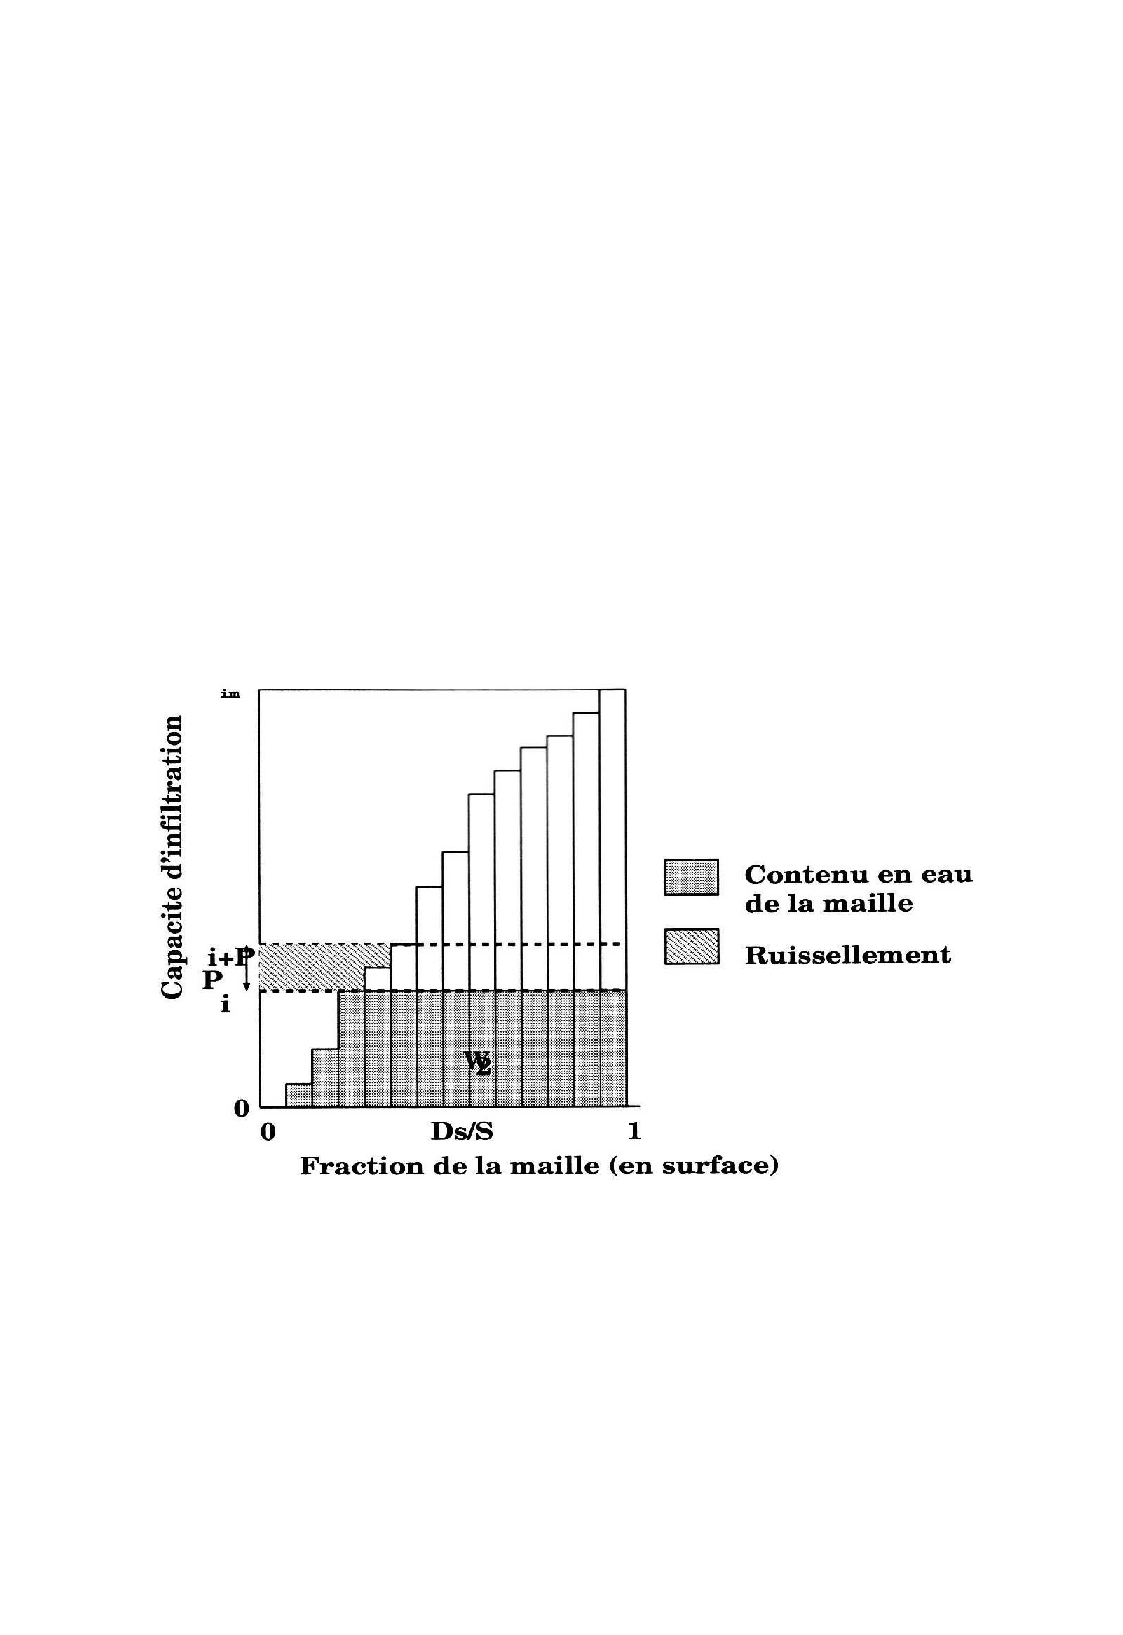
\includegraphics[angle=0, width=12cm, clip=true, trim=1cm 5cm 1cm 7cm]{\EPSDIR/ruisa.pdf}
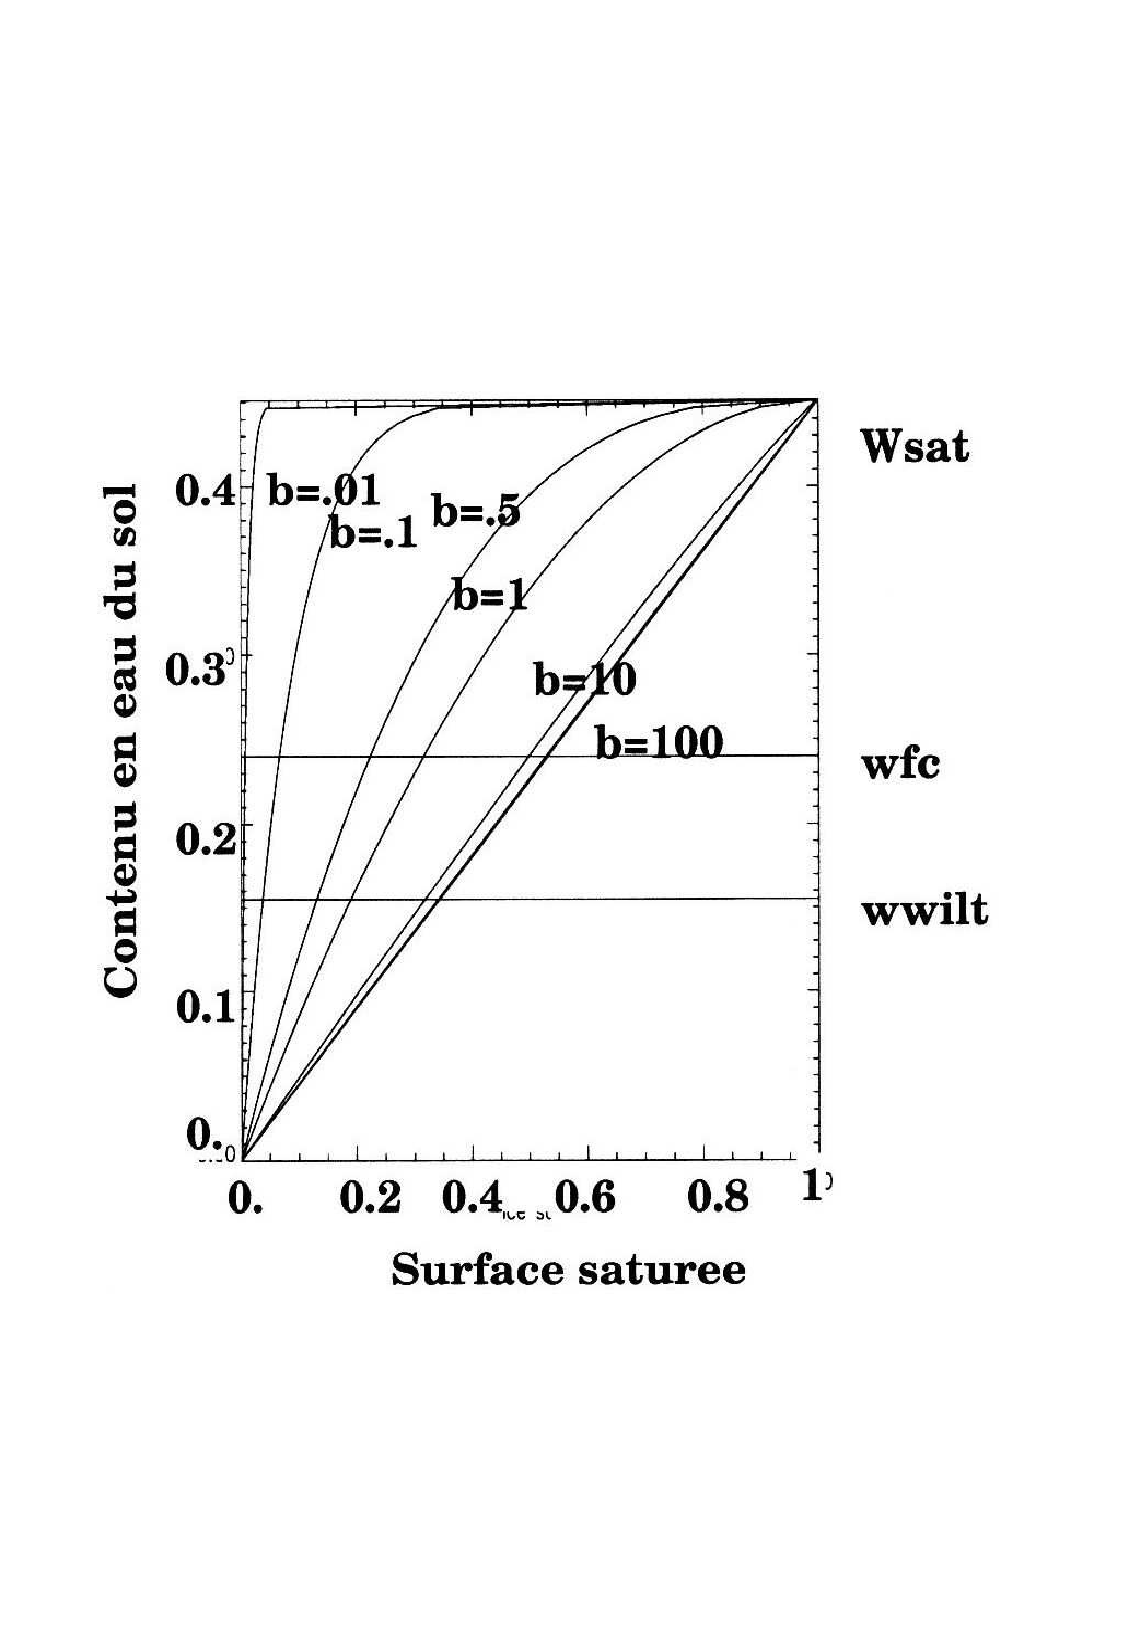
\includegraphics[angle=0, width=7cm,  clip=true, trim=1.5cm 1cm 0cm 4cm]{\EPSDIR/ruisb.pdf}}
\caption{
Simplified scheme of the VIC subgrid runoff.
Left : principles. Right : variation of the saturated proportion of
the grid cell for several values of the soil water content and of the
parameter b in the VIC model. In Isba, the saturated fraction of the
grid is computed between $w_{wilt}$ and $w_{sat}$.
}
\label{fig:vic}
\end{figure}
%%%%%%%%%%%%%%%%%%%%%%%%%%%%%%%%%%%%%%

$i$ is the water content of the non saturated elementary reservoirs (all reservoirs
with a water content below $i$ are saturated). $A(i)$ is the saturated fraction of the cell.
In case of precipitation ($P$), all reservoirs with an infiltration capacity lower than $i + P$
will be filled, and then produce runoff. The runoff is the sum of the contribution of the elementary reservoirs.

In this scheme, the infiltration capacity is given by : 
%
%%%%%%%%%%%%%%%%%%%%%%%%%%%%%%%%%%%%%%%
\begin{equation}
\label{eq:i_m_vic_model}
  i=i_m \left[ 1- (1-A(i))^{\frac{1}{{\rm b}}} \right]  \Longleftrightarrow A(i)=1- \left( 1- \frac{i_0}{i_m}\right)^{\rm b}
\end{equation}
%%%%%%%%%%%%%%%%%%%%%%%%%%%%%%%%%%%%%%%
%
where $A(i)$ is the fraction of the grid cell whose the infiltration capacity is
lower than $i$ ($0 \le A(i) \le 1$), $i_m$ is the
maximum infiltration capacity of the grid cell, and b is the curvature
parameter, which controls the distribution function $A$~:
the runoff is high when b is high, and low when b is small. 

In the grid cell, the runoff is given by :
%
%%%%%%%%%%%%%%%%%%%%%%%%%%%%%%%%%%%%%%%
\begin{equation}
  Q_r = \int_{i}^{i+P} A(i) di = P + \frac{i_m}{b+1} \left[  \left( 1-
      \frac{i+P}{i_m} \right)^{{\rm b}+1} - \left( 1- \frac{i}{i_m}
    \right)^{{\rm b}+1} \right]
\end{equation}
%%%%%%%%%%%%%%%%%%%%%%%%%%%%%%%%%%%%%%%
%
For a water content $w_2$, the saturated fraction of the grid cell (
$A(w_2)$) is given by:
%
%%%%%%%%%%%%%%%%%%%%%%%%%%%%%%%%%%%%%%%
\begin{equation}
\label{eq:a_vic_model}
  A(w_2) = 1 - \left( 1 - \frac{w_2}{w_{sat}} \right)^{\frac{{\rm b}}{{\rm b}+1}}
\end{equation}
%%%%%%%%%%%%%%%%%%%%%%%%%%%%%%%%%%%%%%%
%
After preliminary testing of this parameterization on the Adour watershed, Habets \etal (1999)
found that the parameterization generated too much runoff in summer for dry
soil conditions. To avoid this problem, a threshold was introduced in
the soil wetness, $w_{c,min}$,
below which runoff was not produced. This threshold was set to be the wilting point
($w_{c,min}=w_{wilt}$). Note that this threshold is somewhat arbitrary in terms
of it's relationship to surface runoff. For example, a recent study
using ISBA has shown
that for a tropical catchment the relationship with wilting point is
weak
and a larger threshold value of $w_{c,min}$ produces
optimal results (Getirana et al., 2014\nocite{getirana_ea_2014}). So, $w_{c,min}=w_{wilt}$ should be
used by default, but a different value could be best for a given
catchment or climate (Note, currently $=w_{wilt}$ is hard-coded).


The discretized form of $Q_r$ used within the model can be written as
%
%
%%%%%%%%%%%%%%%%%%%%%%%%%%%%%%%%%%%%%%%%%%%%%%%%%%%%
\begin{subequations}
\begin{align}
\label{qrc}
Q_{r\,{\rm crit}} \,\,=\,\, &
{\left[1 - {\left(w_2-w_{c,min}\right)\over 
\left(w_{sat}-w_{c,min}\right)}\right]}^{1/(1+{\rm b})}
\,-\,
{R_t \Delta t \over \rho_w z_r}
\left[{ 1\over
(1+{\rm b})\left(w_{sat}-w_{c,min}\right)
}\right]
\\
\label{qr}
Q_r \,\,=\,\, & R_t - {\rho_w z_r \over\Delta t}
\Biggr\lbrace
\left(w_{sat}-w_2\right)-
\left(w_{sat}-w_{c,min}\right) 
{\left[{\rm max}\left(0,\,Q_{r\,{\rm crit}}\right)\right]}^{1+{\rm b}}
\Biggr\rbrace
\end{align}
\end{subequations}
%%%%%%%%%%%%%%%%%%%%%%%%%%%%%%%%%%%%%%%%%%%%%%%%%%%%
%
with the constraints:
%
%%%%%%%%%%%%%%%%%%%%%%%%%%%%%%%%%%%%%%%%%%%%%%%%%%%%%%%%
\begin{equation}
\label{qrz}
Q_r \,\,=\,\, 0
\hskip.5in
{\rm if}\hskip.2in
\left(Q_r < 0 \right) 
\hskip.2in {\rm or}\hskip.2in 
\left(w_2 \leq w_{c,min}\right) 
\end{equation}
%%%%%%%%%%%%%%%%%%%%%%%%%%%%%%%%%%%%%%%%%%%%%%%%%%%%%%%%
%
where $R_t$
(m s$^{-1}$) is the through-fall rate (sum of canopy drip, precipitation
and snow-melt). 

\paragraph{TOPMODEL approach}    TOPMODEL (TOPography based MODEL) attempted to combine the important 
distributed effects of channel network topology and dynamic contributing areas for runoff 
generation (Beven and Kirkby (1979)\nocite{beven1979}, Silvapalan \etal (1987)\nocite{Silvapalan1987}). This formalism takes into account 
topographic heterogeneities explicitly by using the spatial distribution of the topographic 
indices, $\lambda_i (m)$, in each grid-cell defined as follows:
%
\begin{equation}
  \lambda_i = \ln\left(a_i / \tan\beta_i \right) 
\end{equation}
%
where $a_i (m)$ is the drainage area per unit of contour of a local pixel, $i$, and $\tan\beta_i$ approximates 
the local hydraulic gradient where $\beta_i$ is the local surface slope. If the pixel has a large drainage 
area and a low local slope, its topographic index will be large and thus, its ability to be 
saturated will be high. Then, this topographic index can be related to a local water deficit, and 
using the spatial distribution of the topographic indices over the grid cell, a saturated fraction, 
$f_{sat}$, inversely proportional to the grid cell mean deficit, $D_t (m)$, can be defined. The 
"coupling" between TOPMODEL and ISBA was proposed by Habets and Saulnier (2001)\nocite{Habets2001} and 
generalized by Decharme \etal (2006).
The active layer used for the ISBA-TOPMODEL coupling is the rooting layer, and not 
the total soil column. TOPMODEL describes generally the evolution of a water storage deficit 
near the soil surface that reacts quasi-instantaneously following rainy events 
(Beven and Kirkby, 1979). In that case, the root zone appears to be a reasonable compromise in ISBA. So, 
the relation between the grid cell mean deficit and the soil moisture computed by ISBA is 
simply expressed as:
%
\begin{equation}
  0 \leq D_t = \left(w_{sat} - w_2 \right) \times d_2 \leq d_0 
\end{equation}
%
where $d_2 (m)$ is the rooting depth and $d_0 (m)$ the maximum deficit computed as the difference 
between the saturation, $w_sat$, and the wilting point, $w_wilt$ :
%
\begin{equation}
  d_0= \left(w_{sat} - w_{wilt} \right) \times d_2
\end{equation}

So for a given rooting soil moisture, $w_2$, a mean deficit, $D_t$, is calculated and it is therefore 
possible to determine the saturated fraction of the grid-cell. The runoff, $Q_{top}$, is thus simply 
given by: $Q_{top} = P_g \times f_{sat}$  where $P_g$ is the throughfall rain rate. For $w_2$ lower than the wilting point, 
the mean deficit is a maximum, $D_t = d_0$ , $f_{sat} = 0$ and no surface runoff occurs. Note that, the 
spatial distribution of the topographic index in each grid-cell can be computed with the three-
parameter gamma distribution introduced by Silvapalan \etal (1987)\nocite{Silvapalan1987}. The three parameters 
are derived from the mean, standard deviation, and skewness of the actual distribution that 
can be done by the HYDRO1K dataset at a 1 km resolution or another database. This 
TOPMODEL approach has been intensively validated both at the regional and global scale 
(Decharme \etal (2006), Decharme and Douville (2006 and 2007)\nocite{Decharme2006a, Decharme2007}).

\paragraph{Horton runoff approach.}   The Horton runoff 
occurs for a rainfall intensity that exceeds the effective maximum infiltration capacity. This 
infiltration excess mechanism tends to dominate the overland flow production in most desert 
or semiarid regions where short rainfall events can be very intense, but also where the absence 
of vegetation and other organic matter prevents the development of a porous soil structure 
through which water can move easily. The development of a thin crust at the soil surface can 
also inhibit the infiltration (arid or frozen soil). So the Horton runoff, $Q_{hort}$, is calculated using 
two infiltration functions following Decharme and Douville (2006): 
%
%%%%%%%%%%%%%%%%%%%%%%%%%%%%%%%%%%%%%%%%%%%%%%%%%
\begin{equation}
		  Q_{hort} = \left(1-\delta_f \right) \times \max\left(0,S_m+ P_g -I_{unf} \right)
                             + \delta_f \max \left(0,S_m+P_g -I_f \right)
\end{equation}
%%%%%%%%%%%%%%%%%%%%%%%%%%%%%%%%%%%%%%%%%%%%%%%%%
%
where $S_m$ is snowmelt, $P_g$ the throughfall rain rate, $I_{unf}$ and $I_f$ the infiltration functions over 
unfrozen and frozen soil, and $\delta_f$ the fraction of the frozen soil. These functions depend on root 
zone soil moisture conditions as well as on soil hydraulic properties. When the Horton runoff (being 
estimated only on the non-saturated fraction of the grid) is activated with the VIC or the TOPMODEL 
runoff, the surface runoff is given by :
%
\begin{equation}
  Q_s = Q_{top\_or\_vic} + \left(1-f_{sat}\right) Q_{hort}
\end{equation}

\paragraph{Treatment of drainage}

The gravitational drainage when $w > w_{fc}$ is given by the following equations 
(Mahfouf and Noilhan, 1996; Boone \etal 1999) :
%
\begin{eqnarray}
  K_2= & \frac{C_3}{\tau}\frac{d_3}{d_2} \mathrm{max}[0,(w_2 - w_{fc})] \\
  K_3= & \frac{C_3}{\tau}\frac{d_3}{d_3 - d_2} \mathrm{max}[0,(w_3 - w_{fc})] 
\end{eqnarray}
%
where $\tau$ is a characteristic time (one day).
$C_3$ is the \emph{force-restore} parameter which account for the speed
at which the humidity profile is restored to the field capacity. This
parameter depends on the hydraulic properties of the soil
(Noilhan and Mahfouf, 1996). 
In ISBA, it can be described by an empirical equation and depends on the proportion of 
clay in the grid cell.
%
\begin{equation}
  C_3 = 5.327 \cdot X^{-1.043}_{clay}
\end{equation}

%\paragraph{Subgrid drainage}    
%	 In the original formulation, the drainage stops below the field capacity $w_{fc}$.
%	 Within the framework of the Safran-Isba-Modcou model Habets \etal (2008)\nocite{Habets2008}
%         a subgrid drainage was introduced in order to account for unresolved aquifers
%	 in the model. A residual drainage was introduced in ISBA. The equations above
%	 are slightly modified :
%	 \begin{eqnarray}
%		 K_2= & \frac{C_3}{\tau}\frac{d_3}{d_2} \mathrm{max}[{w_d}_2,(w_2 - w_{fc})] \\
%		 K_3= & \frac{C_3}{\tau}\frac{d_3}{d_3 - d_2} \mathrm{max}[{w_d}_3,(w_3 - w_{fc})] 
%	 \end{eqnarray}
%
%	 In this formulation, ${w_d}_i$ (for each layer $i$) is expressed as :
%    \begin{equation}
%    	{w_d}_i = w_{drain} max \left( 0, \frac{ min(w_{fc},w_i) - {w_g}_{min}} {w_{fc}-{w_g}_{min}} \right) 
%     \end{equation}
%
%	 where $w_{drain}$ is a parameter to be calibrated, and ${w_g}_{min}$ 
%	 a small parameter to avoid numerical problems.
%
%	 $w_{drain}$ must be calibrated using discharge measurements
%	 during dry periods. See Caballero \etal
%	 (2007)\nocite{Caballero2007},
%
%	 and Habets \etal (2008) for calibration with discharge for the Safran-Isba-Modcou model.


%=========================================================================================================
\subsubsection{Treatment of soil ice}
\label{sec:isba_soil_ice_treatment}
%=========================================================================================================

The inclusion of soil freezing necessitates the addition
of so-called phase change to the thermal and hydrological
transfer equations. In addition,
a freezing/drying wetting/thawing analogy is
used to model changes in the force-restore coefficients
so that they must also be modified accordingly. Terms which have been
added to the baseline ISBA scheme are underlined in this
section, while terms which are modified are denoted using
an $\ast$ superscript.
Additional details related to soil freezing scheme 
can be found in Boone \etal (2000) and Boone (2000)\nocite{Boone2000a}.

The basic prognostic equations
including soil ice are expressed as
%
\begin{eqnarray}
\frac{\partial T_s}{\partial t} &=&
{C_T}^\ast \left[ R_n \,-\, H \,-\, {LE}^\ast \,-\,
L_f(M_s-{\underline{F_{g\,w}}})\right] \,-\,
\frac{2\pi}{\tau}(T_s-T_2)
\,\,\,, \\
%
\frac{\partial T_2}{\partial t} &=&
\frac{1}{\tau}(T_s-T_2)
\,+\,{C_G}^\ast L_f {\underline{F_{2\,w}}}
\,\,\,, \\
%
\frac{\partial w_g}{\partial t} &=&
\frac{1}{ d_1\rho_w} \left[ {C_1}^\ast\left(P_g-E_{g\,l}+M_s \right)
\,-\, {\underline{F_{g\,w}}} \right]
\,-\, \frac{{C_2}^\ast}{\tau}(w_g-{w_{g\,{\rm eq}}}^\ast) \\
& & \hskip2.6in
(w_{{\rm min}} \leq w_g \leq w_{\rm sat}-w_{g\,f})
\,\,\,, \\
%
\frac{\partial w_2}{\partial t} &=&
\frac{1}{ d_p\rho_w}
\left(P_g-{E_{g\,l}}-{E_{tr}}^\ast+M_s-
{\underline{F_{2\,w}}} \right) \,-\,{C_3}{\tau}{\rm max}
(0\,,\,\,w_2-{w_{\rm fc}}^\ast) \\
& & \hskip2.6in
(w_{{\rm min}}\leq w_2 \leq w_{\rm sat}-w_{2\,f})
\,\,\,, \\
%
\frac{\partial w_{g\,f}}{\partial t} &=&
\frac{1}{ d_1 \rho_w} \left(
F_{g\,w} \,-\, E_{g\,f} \right)
\hskip1.35in
(0 \leq w_{g\,f}\leq w_{\rm sat}-w_{{\rm min}} )
\,\,\,, \\
%
\frac{\partial w_{2\,f}}{\partial t} &=&
\frac{1}{ \left(d_2-d_1\right)\rho_w} F_{2\,w}
\hskip1.6in
(0 \leq w_{2\,f}\leq w_{\rm sat}-w_{{\rm min}} )
\,\,\,.
\end{eqnarray}
%
where $w_{g\,f}$ and $w_{2\,f}$ represent the volumetric soil ice content
(m$^3$ m$^{-3}$) in the surface and deep-soil reservoirs, respectively.
The phase change mass and heat sink (source) terms ($F$; kg m$^{-2}$ s$^{-1}$)
are expressed as
%
\begin{eqnarray}
F_{g\,w} &=& \left(1-p_{sng}\right)\,\left( F_{g\,f}
\,-\, F_{g\,m}\right)\,\,\,, \\
%
F_{2\,w} &=& \left(1-p_{sng}\right)\,\left( F_{2\,f}
\,-\, F_{2\,m}\right)\,\,\,,
\end{eqnarray}
%
where the $m$ and $f$ subscripts represent melting and
freezing, respectively.
The freezing and melting phase change terms are formulated using simple
relationships based on the potential
energy available for phase change. They are expressed
for the surface soil layer as
%
\begin{eqnarray}
F_{g\,f} &=& \left(1/\tau_i \right)\,{\rm min} \left[
K_s \,\epsilon_{s\,f} \,{\rm max}(0,\,T_0-T_s)/C_I \, L_f ,\,
\rho_w\,d_1\,\left( w_g-w_{\rm min} \right)
\right]
\,\,\, , \\
%
F_{g\,m} &=& \left(1/\tau_i \right)\,{\rm min} \left[
K_s \,\epsilon_{s\,m} \,{\rm max}(0,\,T_s-T_0)/C_I \, L_f ,\,
\rho_w\,d_1\,w_{g\,f}
\right]
\,\,\, ,
\end{eqnarray}
%
and for the deep soil layer as
%
\begin{eqnarray}
F_{2\,f} &=& \left(\delta_{2\,f}/\tau_i \right)\,{\rm min} \left[
\epsilon_{2\,f} \,{\rm max}(0,\,T_0-T_2)/C_I \, L_f , \,
\rho_w\,\left(d_2-d_1\right)\left( w_2-w_{\rm min}\right)\right]
\,\,\, ,\\
%
F_{2\,m} &=& \left(1/\tau_i \right)\,{\rm min} \left[
\epsilon_{2\,m} \,{\rm max}(0,\,T_2-T_0)/C_I \, L_f , \,
\rho_w\,\left(d_2-d_1\right)\,w_{2\,f}\right]
\,\,\,.
\end{eqnarray}
%
The characteristic time scale for freezing is represented by $\tau_i$ (s).
The phase change efficiency coefficients, $\epsilon$, introduce
a dependence on the water mass available for phase changes
which are expressed as
the ratio of the liquid volumetric water content
to the total soil porosity for freezing,
and the ratio of ice content to the porosity for melting.
The ice thermal inertia coefficient is defined as
$C_I = 2 {\left( {\pi/\lambda_i\,C_i\rho_i\tau} \right)}^{1/2}$
(J m$^{-2}$ K$^{-1}$).
The insulating effect of vegetation is modeled using a coefficient
defined as
%
\begin{eqnarray}
K_s =
\, \left(1-\frac{veg}{ K_2}\right) \left(1-\frac{LAI}{ K_3}\right) \,\,\,,
\end{eqnarray}
%
where the dimensionless coefficients have
the values $K_2\,=\,5.0$ and $K_3\,=\,30.0$ (Giard and Bazile (2000)\nocite{Giard2000}).
The most direct
effect of vegetation cover
is to slow the rate of phase changes for more dense vegetation cover
as energy not used for phase change is assumed to cool/warm the
vegetative portion of the lumped soil-vegetation layer.

The deep-soil phase change (freezing) term
is multiplied by a factor ($\delta_{2\,f}$)
which essentially limits ice production during prolonged
cold periods.  It is defined as 0 if $z_f \geq z_{f\,{\rm max}}$
where
%
\begin{eqnarray}
z_{f\,{\rm max}} &=& 4/\left( {C_G}^\ast\,c_g\right)
\,\,\,
\end{eqnarray}
and the actual depth of ice in the soil is defined as
\begin{eqnarray}
z_f &=& d_2 \, \left(\frac{w_{2\,f}}{ w_{2\,f} + w_2}\right)
\hskip1.in \left(0 \leq z_f < d_2\right)
\end{eqnarray}
%
Ice is assumed to become
part of the solid soil matrix. This is accomplished by
defining the modified porosity
(eg. Johnsson and Lundin (1991)\nocite{Johnsson1991}) as
%
\begin{eqnarray}
{w_{sat}}^\ast = w_{sat} - w_{j\,f}
\end{eqnarray}
%
where $j$ corresponds to the surface ($g$) or sub-surface ($2$)
soil water reservoirs.
This, in turn, is used to modify the force-restore coefficients
(see Boone \etal, 2000, for more details).

As a final note, more recently an option to this simple method to
compute the phase changes has been
added based on the Gibbs-free energy approach. It is especially
adapted for the DuFfusion (DF) version of ISBA (see
Section~\ref{sec:isba_diffusion_soil}), but it can also be used with
the FR approach. See Section~\ref{sec:isba_soil_ice} for more details.
But the soil ice modification to the porosity etc. remains as described
in this Section for both phase change options.

%=========================================================================================================
%=========================================================================================================
\subsection{Diffusive approach}
\label{sec:isba_diffusion_soil}
%=========================================================================================================
%=========================================================================================================

%
%=========================================================================================================
\subsubsection{Governing Equations}
%=========================================================================================================
%
The governing equations for the heat and mass transfer
from the surface down through the soil column for the snow-free
case are expressed as (Boone \etal 2000; Decharme \etal 2011):
%
\begin{eqnarray}
c_h\frac{\partial T_g}{ \partial t } \,\,&=&\,\,
\frac{\partial G }{ \partial z} 
\,+\,\Phi \label{tdifsn} \\
%
\frac{\partial w_l }{\partial t} \,\,&=&\,\,
-\frac{\partial F}{\partial z} \,-\, \frac{\Phi}{ L_f \rho_w}\,-\, \frac{S_l}{ \rho_w}
\hskip.8in (w_{min}\,\leq\, w_l\,\leq\,w_{sat}-w_i) \label{cont1}\\
%
\frac{\partial w_i}{\partial t} \,\,&=&\,\,
\frac{\Phi}{ L_f \rho_w} \,-\, \frac{S_i}{ \rho_w}
\hskip1.32in (0 \,\leq\, w_i\,\leq\,w_{sat}-w_{min})\label{ice} 
\end {eqnarray}
%
Eq.~(\ref{tdifsn}) is the vertical component of the 
heat transfer equation: heat flow is induced
along the thermal gradient and due to convection,
$c_h$ is the total heat capacity
(J ${\rm m^{-3}\,K^{-1}}$): it is represented by
a lumped heat capacity in the surface layer, and by
the soil heat capacity ($c_g$) in the sub-surface layers.
$\lambda$ is the thermal conductivity (W ${\rm m^{-1}\,K^{-1}}$),
$F$ is the vertical flow rate of water (m ${\rm s^{-1}}$),
$T_g$ is the composite soil-vegetation  temperature (K) at the surface
and the soil temperature only for sub-surface layers, $\Phi$ (${\rm J \, m^{-3}\,s^{-1}}$)
is a latent heat
source/sink resulting from phase transformation of soil water,
and the soil depth, $z$ (m), is increasing downward.

$w_l$ and $w_i$ in Eq.s~(\ref{cont1}) and (\ref{ice}) 
represent
the volumetric liquid water and liquid water equivalent ice contents
of the soil (${\rm m^3 \, m^{-3}}$), respectively. They are
related to the total volumetric water content 
(${\rm m^3 \,m^{-3}}$) through
%
\begin{equation} \label{totalsoilwater}
w \,\,=\,\,w_l \, +\, w_i
\,\,\, .
\end{equation}
%
In Eq.~(\ref{cont1}), 
$S_l$ (evapotranspiration, lateral inflow) 
and $S_i$ (sublimation) represent external sources/sinks
(kg m$^{-3}$ s${-1}$), 
of the liquid and ice liquid equivalent soil water, respectively, 
$L_f$ is the latent heat of fusion 
(3.337 ${\rm \times {10}^5 \,J\,{kg}^{-1}}$),
and $\rho_w$ is the density
of liquid water (1000 kg ${\rm m^{-3}}$).
The total soil porosity is 
$w_{sat}$ (${\rm m^3 \, m^{-3}}$), and
$w_{min}$ is a minimum liquid water threshold
(0.001 ${\rm m^3 \, m^{-3}}$).

The phase change terms on the right-hand sides of Eq.s~(\ref{cont1}) 
and (\ref{ice}) represent a mass
transfer between the solid and liquid phases
of the soil water. 
The continuity equation for the total
soil volumetric water content is obtained by
adding Eq.s~(\ref{cont1}) and (\ref{ice}) and then
substituting Eq.~(\ref{totalsoilwater}) 
into the resulting expression to have
%
%%%%%%%%%%%%%%%%%%%%%%%%%%%%%%%%%%%%%%%%%%%%%%%%%%%%%%%%
\begin{equation}
%\label{}
\frac{\partial w}{\partial t} \,\,=\,\,
-\frac{\partial F}{\partial z} \,-\, \frac{1}{\rho_w}\left(S_i\,+\, S_l\right)
\hskip.8in 
\left(w_{min}\,\leq\, w\,\leq\,w_{sat}\right)
\end{equation}
%%%%%%%%%%%%%%%%%%%%%%%%%%%%%%%%%%%%%%%%%%%%%%%%%%%%%%%%
%

%=========================================================================================================
\subsubsection{Surface and soil heat transfer}
%=========================================================================================================
%
Heat flow is along the thermal gradient,
so that the soil heat flux (W m$^{-2}$) can be expressed as
%
%%%%%%%%%%%%%%%%%%%%%%%%%%%%%%%%%%%%%%%%%%%%%%%%%%%%%%%%
\begin{equation}
\label{gxxx}
G = \lambda \frac{\partial T}{\partial z}
\end{equation}
%%%%%%%%%%%%%%%%%%%%%%%%%%%%%%%%%%%%%%%%%%%%%%%%%%%%%%%%
%
The soil thermal conductivity and heat capacity 
are expression as functions of soil properties
and moisture. The parameterizations are described below.

\paragraph{Calculation of the thermal properties}
%
The thermal heat capacity and thermal conductivity
are parameterized as functions
of the soil moisture and texture by most SVAT schemes.
SVAT schemes which participated in
PILPS-phase2c predicted, in general, ground heat fluxes
poorly, which is most likely related to thermal 
conductivity parameterization Liang \etal (1996)\nocite{Liang1996}. 
ISBA uses the formulations from McCumber and Pielke (1981 : MP81)\nocite{McCumber1981}
together with parameter values from Clapp and Hornberger (1978)
to evaluate the heat capacity and thermal conductivity
(Noilhan and Planton, 1989), but
it is known that thermal conductivity estimates using the 
MP81 model tend to be too large for wet conditions (nearing saturation)
while underestimating thermal conductivity for dry soils.
Also, there is no consideration of frozen soils in this formulation.
There are several alternatives to using the MP81 
model for thermal conductivity, and
one such method is that discussed in Peters-Lidard \etal (1998)\nocite{Peters-Lidard1998}.
%
The layer-averaged soil heat capacity can be written as
%
\begin{equation}\label{heatcapacity}
c_{g\,j} \,\,=\,\, (1-w_{sat})C_{soil}\rho_{soil} 
\,+\, w_{l\,j} c_w \, +\, w_{i\,j} c_i 
\end{equation}
%
where 
$c_i$ and $c_w$ are the heat capacities of ice and liquid water, 
(J ${\rm K^{-1} \, m^{-3}}$).
$C_{soil}$ is the specific heat of the soil (J ${\rm {kg}^{-1}}
\, K^{-1}$) and $\rho_{soil}$ represents the soil dry density.
The specific heat ($C_{soil}$) value of 733 J ${\rm {kg}^{-1} \, K^{-1}}$
for soil minerals/quartz from
Peters-Lidard \etal (1998) is used.
%The dry density is sometimes measured, but it can also be
%estimated from the soil porosity assuming the same solids unit
%weight (Peters-Lidard \etal 1998):
%
%%%%%%%%%%%%%%%%%%%%%%%%%%%%%%%%%%%%%%%%%%%%%%%%%%%%%%%%
%\begin{equation}
%\rho_{soil} \,\,=\,\, (1-w_{sat})\rho_{solids} 
%\end{equation}
%%%%%%%%%%%%%%%%%%%%%%%%%%%%%%%%%%%%%%%%%%%%%%%%%%%%%%%%
%
where $\rho_{soil}$ represents the unit weight of the solids 
(2700 kg ${\rm m^3}$).
%
The heat capacity of air in the soil is neglected in
Eq.~(\ref{heatcapacity}).

For fine soils or coarse frozen soils, the method of Johansen (1975)\nocite{johansen1975} was 
shown by Farouki (1986)\nocite{farouki1986} to be the most accurate relative to other commonly
used methods for calculating thermal conductivity.
Following Peters-Lidard \etal (1998),
the thermal conductivity is calculated as the weighted sum of
the dry and saturated thermal conductivities from (Johansen, 1975)
%
\begin{equation}\label{condpl}
\lambda \,\,=\,\, K_e \,\lambda_{sat} \,+\,(1-K_e)\,\lambda_{dry}
\end{equation}
%
where $K_e$ is the non-dimensional Kersten number.

The dry thermal conductivity is defined as
%
%%%%%%%%%%%%%%%%%%%%%%%%%%%%%%%%%%%%%%%%%%%%%%%%%%%%%%%%
\begin{equation}
\label{conddry}
\lambda_{dry} \,\,=\,\, 
\frac{0.135 \rho_{soil} \,+\,64.7}
{\rho_{solids} \,-\,0.947 \rho_{soil}}
\end{equation}
%%%%%%%%%%%%%%%%%%%%%%%%%%%%%%%%%%%%%%%%%%%%%%%%%%%%%%%%
%
where $\lambda_{dry}$ is in W ${\rm m^{-1}}\, K^{-1}$.
%
For crushed rock, 
%
%
%%%%%%%%%%%%%%%%%%%%%%%%%%%%%%%%%%%%%%%%%%%%%%%%%%%%%%%%
\begin{equation}
\lambda_{dry} \,\,=\,\, 0.039 \, {w_{sat}}^{-2.2}
\end{equation}
%%%%%%%%%%%%%%%%%%%%%%%%%%%%%%%%%%%%%%%%%%%%%%%%%%%%%%%%
%
The saturated thermal conductivity is written as
%
\begin{equation}\label{condsat}
\lambda_{sat} \,\,=\,\, 
{\lambda_{soil}}^{(1-w_{sat})}\,
{\lambda_{i}}^{(w_{sat}-\chi_u)}\,
{\lambda_{w}}^{\chi_u}
\end{equation}
%
where $\chi_u$ represents the unfrozen volume fraction of the soil.
It is defined as
%
%
%%%%%%%%%%%%%%%%%%%%%%%%%%%%%%%%%%%%%%%%%%%%%%%%%%%%%%%%
\begin{equation}
\chi_u \,\,=\,\,w_{sat}\left(w_l/w\right)
\hskip.5in
\left(0 \,\leq\,\chi_u \,\leq\,w_{sat}\right)
\end{equation}
%%%%%%%%%%%%%%%%%%%%%%%%%%%%%%%%%%%%%%%%%%%%%%%%%%%%%%%%
%
%
In Eq.~(\ref{condsat}),
$\lambda_{i}$ represents the thermal conductivity of ice
(2.2 W ${m^{-1}\,K}$), $\lambda_{w}$ represents the thermal 
conductivity of water
(0.57 W ${m^{-1}\,K}$), and
the thermal conductivity of solids is written as
%
%
%%%%%%%%%%%%%%%%%%%%%%%%%%%%%%%%%%%%%%%%%%%%%%%%%%%%%%%%
\begin{equation}
\label{condsolids}
\lambda_{soil} \,\,=\,\, {\lambda_q}^q \,{\lambda_o}^{1-q}
\end{equation}
%%%%%%%%%%%%%%%%%%%%%%%%%%%%%%%%%%%%%%%%%%%%%%%%%%%%%%%%
%
%
The quartz content ($0 \leq q \leq 1$) is non-dimensional.
It is fit as a function of sand (following the method of
Noilhan and Lacarr\`{e}re (1995)\nocite{Noilhan1995}
using the data from PL98:
%
\begin{equation}\label{quartzr}
q \,\,=\,\, 0.038 \,+\, 0.0095 \,X_{\rm sand} 
\end{equation}
%
where the fraction of the soil comprised by sand
is represented by $X_{\rm sand}$ (\%). The relation is
shown graphically in Fig.~(\ref{quartzf}).
The thermal conductivity of quartz is represented as
$\lambda_q$ (7.7 W ${m^{-1}\,K}$), and 
the thermal conductivity of other minerals is represented as
$\lambda_o$ (W ${m^{-1}\,K}$) where
%
%%%%%%%%%%%%%%%%%%%%%%%%%%%%%%
\begin{equation}
%
\lambda_o \,\, = \,\, \Bigg\lbrace
%
\begin{matrix}
2 & q > 0.2
\\
3 & q \leq 0.2
%
\end{matrix}
%
\end{equation}
%%%%%%%%%%%%%%%%%%%%%%%%%%%%%%
%
\begin{figure}[h]
		 \begin{center}
		 \psfig{figure=\EPSDIR/quartz.pdf,width=8cm}
		 \caption{The relation between quartz content ($q$) and
sand fraction ($X_{\rm sand}$) of the soil (\%).
The relationship between quartz and sand content
is described by Eq.~(\ref{quartzr}).
The data are plotted using the values of $q$ from
Peters-Lidard \etal (1998) and the sand fraction
from Cosby \etal (1984).}
\label{quartzf}
		 \end{center}
\end{figure}
\nocite{Cosby1984}


The Kersten number is written as
%
%
%%%%%%%%%%%%%%%%%%%%%%%%%%%%%%
\begin{equation}
%
K_e \,\, = \,\, \Bigg\lbrace
%
\begin{matrix}
0.7 \, {\rm log}_{10}\,\theta \,+\,1.0 & 
\theta > 0.05 \,\, ({\rm coarse})
\\
{\rm log}_{10}\,\theta \,+\,1.0 & 
\theta > 0.10 \,\, ({\rm fine})
%
\end{matrix}
%
\end{equation}
%%%%%%%%%%%%%%%%%%%%%%%%%%%%%%
%
and for frozen soils it is
%
\begin{equation}\label{kerstfrz}
K_e = \theta 
\end{equation}
%
where $\theta$ is the degree of saturation ($w/w_{sat}$) of the soil
layer. Because use of Eq.~(\ref{kerstfrz}) can result in
a large jump in $K_e$ as a soil begins to freeze, the following expression
is used for partially frozen fine soils:
%
\begin{equation}\label{kerstfrzp}
K_e \, = \, (w_l/w)\left({\rm log}_{10}\,\theta\,+\,1.0\right)
 \,+\, (w_i/w)\theta
\end{equation}
%
The same weighting scheme in Eq.~(\ref{kerstfrzp})
can be used for coarse soils as well. 

\paragraph{Numerical discretization of the soil heat equation}
%
%Integrating the heat transfer equation [Eq.~(\ref{tdifsn})]
%downward into the soil to obtain the 
%average temperature for $N$ soil layers:
%%
%\begin{equation}\label{inttdif}
%\int_{-z_j}^{-z_{j-1}} 
%c_h 
%\frac{\partial T_g}{\partial t } dz \,\,=\,\,
%\int_{-z_j}^{-z_{j-1}} 
%%{\partial }{ \partial z} \lambda {\partial T }{ \partial z} dz
%\frac{\partial G}{\partial z} dz
%%%\,+\,\int_{-z_j}^{-z_{j-1}} {\partial (F\,T)}{\partial z} dz
%\,+\,\int_{-z_j}^{-z_{j-1}} \Phi dz
%\end{equation}
%
%where
%
%\begin{equation}\label{tavglyr}
%T_{g,\,j} \,\,=\,\, \frac{1}{\Delta z_j} \int_{-z_j}^{-z_{j-1}}
%\,T_g dz
%\end{equation}
%
%$T_{g,\,j}$ is the layer averaged temperature ($j=1,...,N$),
%the vertical index $j$ is increasing downward and
%$\Delta z_j$ is defined as $z_j - z_{j-1}$. 

%Carrying out the integration in Eq.~\ref{inttdif} using 
%the operator in Eq.~\ref{tavglyr} yields
%
The governing equations for heat transfer within the soil discretized
in $N_g$ layers are described using the classical one-dimensional Fourier
law and are written as:
%
%%%%%%%%%%%%%%%%%%%%%%%%%%%%%%%%%%%%%%ù
\begin{subequations}
\begin{align}
\label{teq}
\Delta z_j c_{g\,j}\frac{\partial T_{g,\,j}}{\partial t } \,\,=&\,\,
G_{j-1} \,-\, G_j 
\,+\,\Delta z_j\,\Phi_j
\hskip2.5in
\forall = 2,N_g
\\
\label{teq_flux}
\Delta z_j c_{g\,j}\frac{\partial T_{g,\,j}}{\partial t } \,\,=&\,\,
\frac{{\overline\lambda}_{j-1}}{\Delta {\tilde z}_{j-1}}
\left( T_{g,\,j-1} \,-\, T_{g,\,j}\right)
\,-\,
\frac{{\overline\lambda}_j}{\Delta {\tilde z}_j}
\left( T_{g,\,j} \,-\, T_{g,\,j+1}\right)
\,+\,\Delta z_j\,\Phi_j
%
\end{align}
\end{subequations}
%%%%%%%%%%%%%%%%%%%%%%%%%%%%%%%%%%%%%%ù
%
where the heat conduction flux (W m$^{-2}$) 
is therefore defined as
%
%%%%%%%%%%%%%%%%%%%%%%%%%%%%%%%%%%%%%%ù
\begin{equation}
\label{teq_flux}
G_j \,\,=\,\,
\frac{{\overline\lambda}_j}{\Delta {\tilde z}_j}
\left( T_{g,\,j} \,-\, T_{g,\,j+1}\right)
%
\end{equation}
%%%%%%%%%%%%%%%%%%%%%%%%%%%%%%%%%%%%%%ù
%
$\Delta z_j$ (m) is the thickness of the layer $j$,
$\Delta {\tilde z}_j=\left(\Delta z_j+\Delta z_{j+1}\right)/2$ 
is the thickness (m) between two consecutive layer mid-points or nodes,
$C_G$ is the soil thermal inertia at the surface (J m$^{-1}$
kg$^{-2}$),
$c_{g\,j}$ is the total soil heat capacity(J m$^{-3}$ K$^{-1}$), and
${\overline\lambda}_j$ (W m$^{-1}$ K$^{-1}$)
is the inverse-weighted arithmetic mean of the soil thermal conductivity 
at the interface between two consecutive nodes
expressed as:
%
%%%%%%%%%%%%%%%%%%%%%%%%%%%%%%%%%%%%%%%%%%%%%%%%%%
\begin{equation}\label{thckwtdif}
{\overline \lambda}_j \,\,=\,\, 
\frac{\Delta z_{j} + \Delta z_{j+1}}
{\left(\Delta z_{j+1}/\lambda_{j+1}\right) \,+\,
\left(\Delta z_{j}/\lambda_{j}\right)}
\,\,\, .
\end{equation}
%%%%%%%%%%%%%%%%%%%%%%%%%%%%%%%%%%%%%%%%%%%%%%%%%%
%
%The convective heat flow term is parameterized following 
%Pitman et al. (1991) as
%%
%$$ G_{c\,j} \,\,=\,\, 
%{2\,c_w\,F_{j-1}\left( T_j-T_{j-1}\right)
%}{ \left( \Delta z_j + \Delta z_{j-1}\right)}
%\,\,\, ,\eqno\label{heatconv}$$
%%
%using the upwind difference scheme
%where $F_{j-1}$ represents the soil water flux accross
%the level $z=z_{j-1}$. 
In general, the contribution of convective heating to the local
soil temperature change is relatively small and can be neglected.
Vapor transfer effects have been incorporated and are currently
being tested: they are not outlined here.
%This term is retained in this formulation, however, as it could
%become important for cases such as the warming of soil
%due to the infiltration of snow melt.
%Note that the values of thermal conductivity and heat
%capacity are held constant over the time step, which is
%a reasonable approximation as long as time steps are not
%too large. 
The model grid configuration is shown in Fig.~\ref{grid}.
The shaded region at the surface represents a vegetation/biomass/litter
layer. The prognostic variables ($T_{g,\,j}$, $w_l$, and $w_i$) 
are shown (water store variables
will be discussed in subsequent sections).

\begin{figure}[h]
		 \begin{center}
		 \psfig{figure=\EPSDIR/tgrid_new.ps,width=10cm}
		 \caption{The model grid configuration: soil prognostic variables
temperature ($T_{g,\,j}$), liquid volumetric water content
($w_{l\,j}$) and volumetric ice content ($w_{i\,j}$) 
are layer mean quantities. The soil heat ($G_j$) and liquid
water fluxes ($F_j$) are evaluated at each level, $z_j$.
The surface energy budget is evaluated defining $T_s = T_{g,\,1}$.
The shaded region at the surface represents a vegetation/biomass/litter.
The soil depth, $z$, is increasing downward (away from the atmosphere).}
		 \label{grid}
		 \end{center}
\end{figure}


\paragraph{Boundary conditions}


Upper boundary condition: 
%
To be consistent with the ISBA-FR surface energy budget, the surface
temperature evolves according to the heat storage in the
soil/vegetation composite and to the thermal gradient between the
surface (the same fine superficial layer than for ISBA-FR) and the
second layer (Boone \etal ,2000\nocite{Boone2000}).
Accordingly, the surface temperature is defined as
%
%%%%%%%%%%%%%%%%%%%%%%%%%%%%%%%%%%%%%%%%%%%%%%%%%%
\begin{subequations}
\begin{align}
%
\label{eq:tsfc}
\frac{1}{C_T} \frac{\partial T_{g,1}}{\partial t} \,\,=&\,\,
G_0 \,+\, \Delta z_1 \,\Phi_1 \,-\, \frac{C_G}{C_T}
\frac{{\overline\lambda}_1}{\Delta {\tilde z}_1}\left(
  T_{g,1} - T_{g,2}\right) \\
%
\label{eq:tsfc_b}
\frac{\partial T_{g,1}}{\partial t} \,\,=&\,\,
C_T \left( R_n \,-\, H \,-\, LE \,+\, \Delta z_1 \,\Phi_1 \right) \,-\, 
C_G \, \frac{{\overline\lambda}_1}{\Delta {\tilde z}_1}
\left( T_{g,1} - T_{g,2}\right) 
%
\end{align}
\end{subequations}
%%%%%%%%%%%%%%%%%%%%%%%%%%%%%%%%%%%%%%%%%%%%%%%%%%
%
where the
flux between the atmosphere and the surface
is represented by $G_0$ (W m$^{-2}$).
This definition of the prognostic equation for $T_{g,1}$
is similar to that presented by
Bhumralkar (1975)\nocite{Bhumralkar1975} and Blackadar (1979)\nocite{Blackadar1976}. It is the same as
the standard Force-Restore method of Noilhan and Planton (1989)\nocite{Noilhan1989}
if $G_1$ is expressed as a restore term.
The thermal inertia coefficient for the composite surface
layer is expressed as
%
%
%%%%%%%%%%%%%%%%%%%%%%%%%%%%%%%%%%%%%%%%%%%%%%%%%%%%%%%%
\begin{equation}
C_T = {\frac{1}{\left(veg/C_V\right)+\left[(1-veg)/C_G\right]}}
\end{equation}
%%%%%%%%%%%%%%%%%%%%%%%%%%%%%%%%%%%%%%%%%%%%%%%%%%%%%%%%
%
%
where $veg$ represents the vegetation cover fraction.
The thermal inertia for the vegetation ($C_V$) can
be case or species dependent. By default, it is computed as
%
%%%%%%%%%%%%%%%%%%%%%%%%%%%%%%%%%%%%%%%%%%%%%%%%%%%%%%%%
\begin{equation}
C_V = \frac{1}{C_{V,ref} + c_w\,W_r}
\end{equation}
%%%%%%%%%%%%%%%%%%%%%%%%%%%%%%%%%%%%%%%%%%%%%%%%%%%%%%%%
%
where $W_r$ (kg m$^{-2}$) is the vegetation interception 
reservoir water storage
and $C_{v,ref}$ (J K$^{-1}$ m$^{-2}$) the reference or baseline
vegetation heat capacity (defined by the user or ECOCLIMAP)
set by default to $1\times 10^4$ J K$^{-1}$ m$^{-2}$ for low
vegetation 
and $2\times 10^4$ J K$^{-1}$ m$^{-2}$ for forests.
%
The soil thermal inertia (J K$^{-1}$ m$^{-2}$) is
defined as
%
%%%%%%%%%%%%%%%%%%%%%%%%%%%%%%%%%%%%%%%%%%%%%%%%%%%%%%%%
\begin{equation}
C_G = \frac{1}{c_{g,1}\,\Delta z_1}
\end{equation}
%%%%%%%%%%%%%%%%%%%%%%%%%%%%%%%%%%%%%%%%%%%%%%%%%%%%%%%%
%
where $c_{g,1}$ is the heat capacity of the first soil layer
(J K$^{-1}$ m$^{-3}$: Eq.~\ref{heatcapacity}).
The uppermost soil thickness, $\Delta z_1$, must be chosen to be sufficiently
thin in order to be consistent with the daily surface temperature
cycle (i.e., 0.01 m by default). 
%
%%%%%%%%%%%%%%%%%%%%%%%%%%%%%%%%%%%
%
%The thermal conductivity of the surface layer is represented by $\lambda_s$.
%There is an option 
%to include the effects of a vegetation/mulch/thin biomass litter
%layer using:
%
%
%%%%%%%%%%%%%%%%%%%%%%%%%%%%%%%%%%%%%%%%%%%%%%%%%%%%%%%%
%\begin{equation}
%\lambda_s = \left[ 1 - veg \left( 1-f_v \right)\right] \lambda_1 
%\end{equation}
%%%%%%%%%%%%%%%%%%%%%%%%%%%%%%%%%%%%%%%%%%%%%%%%%%%%%%%%
%
%where $f_v$ is a reduction factor for the surface layer
%thermal condictivity due to the presence of mulch or organic material.
%The value of this parameter ranges between $0 < f_v \leq 1$, depending upon the
%insulating effect of the material. Following from the ideas of Gonzalez-Sosa \etal (2001)\nocite{Gonzalez-Sosa2001},
%it is assumed that the humidity effects dominate the mulch thermal conductivity.
%Based on the aforementioned work at MUREX,
%$f_v$ is currently assigned a value of 0.10 (meaning
%the mulch thermal conductivity is roughly a tenth of that corresponding
%to the soil). The impact of assuming a lower thermal conductivity for
%the mulch layer is to increase the insulation of the soil 
%(relative to a baresoil case) thereby increasing the surface
%energy (which can then increase the surface temperature diurnal wave 
%amplitude, augment the surface fluxes, etc.) and diminishing the
%thermal wave penetration depth within the soil.
%
In the limit when there is no vegetation (i.e., $veg$ = 0), the
thermal inertia coefficient collapses into $1/C_T = \Delta z_1 c_g$
%and $\lambda_s=\lambda_1$
so that Eq.~\ref{eq:tsfc} takes on exactly the same form as the sub-surface soil
temperature equations. 
%When the mulch-layer option is inactive, then
%$\lambda_s = \lambda_1$.


Lower boundary condition:
%
The average temperature for the lowest layer is 
written using Eq.(\ref{teq}) as
%
%
%%%%%%%%%%%%%%%%%%%%%%%%%%%%%%%%%%%%%%%%%%%%%%%%%%%%%%%%
\begin{equation}
\label{teqn}
\frac{\partial T_{N}}{\partial t} \,\,=\,\,
\frac{( G_{N-1} \,-\, G_N )}{c_{g\,N}\,\Delta z_N}
\end{equation}
%%%%%%%%%%%%%%%%%%%%%%%%%%%%%%%%%%%%%%%%%%%%%%%%%%%%%%%%
%
where the heat flux from below $z_N$ is
assumed to be negligible, resulting in a
zero-flux lower boundary condition (i.e. $G_N = 0$).
Note that in order for this assumption to be valid,
$z_N$ must be sufficiently large (deep). 
The annual temperature wave penetration
depth is, in general, on the order of several meters
(eg., Figs~\ref{wave_figMP} and \ref{wave_fig}), so that
$z_N$ must be at least this deep in oder to accurately model the 
soil temperature profile at time scales of an annual
cycle or more.
%
An alternate method to increasing the soil depth
is to specify the lower boundary flux using an annual
mean soil temperature and an appropriate scaling depth
(Lynch-Stieglitz, 1994\nocite{Lynch-Stieglitz1994}). 
%The flux lower boundary condition
%is written as
%%
%$$ G_N \,\,=\,\,\lambda_N \,
%{\left(T_N\,-\,{\overline T}\right)}{
%\left[ z_a\,-\,(z_N+z_{N-1})/2\right]}
%\,\,\,,\eqno\label{lowerbcflx}$$
%%
%where ${\overline T}$ represents the mean annual soil
%temperature (which can possibly change as a function of year)
%and $z_a$ is the corresponding scaling depth.
This depth can be estimated as the annual wave penetration depth
[see Eq.~(\ref{wavedeptha})]. The only drawback 
%to Eq.~(\ref{lowerbcflx}) 
is that the mean annual soil temperature
and the annual wave penetration depth 
must be known {\it a priori}. The advantages are that less model
layers can be used (a lower total model depth) thereby
reducing computational expense and memory/storage requirements,
and the soil temperature profile is ``constrained'' to some extent
by observational data. 
%
Currently in the model, there is an
option to apply a prescribed $T^\ast$ (either as
a constant or varying in time)
at $z_N$ 
%(so that $z_a$ in the above expression is set to 0):
%
%
%%%%%%%%%%%%%%%%%%%%%%%%%%%%%%%%%%%%%%%%%%%%%%%%%%%%%%%%
\begin{equation}
\label{lowerbcflxn}
G_N \,\,=\,\,\lambda_N \,
\frac{\left[T_N\,-\,T^\ast\left( z=z_N\right)\right]}
{\left(z_N+z_{N-1}\right)/2}
\end{equation}
%%%%%%%%%%%%%%%%%%%%%%%%%%%%%%%%%%%%%%%%%%%%%%%%%%%%%%%%
%
But note that $G_N=0$ is the default. Recently the soil depth has
been extended for thermal computations in order to ensure that this
approximation is reasonable: see Decharme \etal (2016) for details.


\paragraph{Vertical grid}
%
The soil model grid levels do not necessarily
have constant spacing. The assumption that the 
vertical temperature gradients are largest near the surface and 
smaller deeper in the soil indicates that the grid spacing can
increase with increasing soil depth.
It is of interest to specify the first grid level
%to be approximately the penetration depth of the diurnal temperature wave. 
to be thin enough to resolve the diurnal temperature wave.
An estimate of this depth is calculated 
using conductivity calculated by Eq.~(\ref{condpl})
for thawed soils with the relation for wave penetration depth
from Dickinson (1988)\nocite{Dickinson1998}:
%
\begin{equation}\label{wavedepth}
z_d \,\,=\,\, {\left( \frac{\lambda_1 \,\tau}{c_{g\,1}\,\pi}\right)}^{1/2}
\end{equation}
%
Since the diurnal wave penetration depth ($z_d$) is a function
of soil moisture and texture, an
average or maximum value could also be used to a good
approximation: this value might represent the $z_d$
depth for the average soil moisture etc. 
The diurnal wave penetration
depths computed using Eq.~(\ref{wavedepth}) 
are shown in Fig.~(\ref{wave_fig}). The depth $z_d$ is
plotted as a function of the normalized volumetric water content
defined as
%
\begin{equation}\label{normwat}
w_{norm} \,\,=\,\, \frac{w\,-\,w_{wilt}}{w_{sat}\,-\,w_{wilt}}
\hskip.5in (0 \,\leq \, w_{norm} \,\leq \,1) 
\end{equation}
%
The $z_d$ depth usually
ranges from 12-18 cm for most soils across their nominal range
of soil moisture: values in the range from 12-15 cm
could be used for most general cases. 
%
It is of interest to compare the method of Johansen to 
the method of McCumber and Pielke (1981)\nocite{McCumber1981} 
which is used by many surface
vegetation atmosphere transfer (SVAT) schemes including ISBA (Noilhan
and Planton, 1989\nocite{Noilhan1989}).
The $z_d$ values computed using the method of 
McCumber and Pielke (1981)\nocite{McCumber1981}
together with the soil classification and hydrological parameter values
For the force-restore
method used by ISBA, this variability in $z_d$ is accounted for as
there are no fixed soil depths which effect the diurnal cycle.
But when using a fixed grid geometry, as is the case for the diffusion
method outlined here, $z_d$ calculated from the method of Johansen 
is more consistent with a fixed grid geometry.
%
These depths represent the depth to which the diurnal wave is felt:
but to represent the diurnal
cycle of the soil surface or soil-vegetation composite surface
accurately in terms of phase and amplitude, the uppermost layer should
be considerably thinner: in ISBA the uppermost thickness is chosen as a
compromise between thickness, numerical stability (time step) and
processes (both hydrological and thermal): see below for more details.

\begin{figure}[h]
		 \begin{center}
		 \psfig{figure=\EPSDIR/wavedepthMPNP.pdf,width=8cm}
		 \caption{The diurnal temperature wave penetration depths
($z_d$) for the 11 soil classes from Clapp and Hornberger (1978).
Depths are plotted as a function of normalized soil water content
[Eq.~(\ref{normwat})].
Thermal conductivity is calculated using the method of McCumber and Pielke (1981)
together with soil hydraulic parameter values from Clapp and Hornberger (1978).
Soil depths are in m.}
		 \label{wave_figMP}
		 \end{center}
\end{figure}
\begin{figure}[h]
		 \begin{center}
		 \psfig{figure=\EPSDIR/wavedepthdaPL98.pdf,width=8cm}
		 \caption{The diurnal and annual soil temperature wave penetration depths
($z_d$) for the 11 soil classes from Clapp and Hornberger (1978).
Depths are plotted as a function of normalized soil water content
[Eq.~(\ref{normwat})].
Thermal conductivity is calculated using the method of Johansen (1975)
as presented by Peters-Lidard \etal (1998).
Soil depths are in m: $z_d$ should be used as a guild-line for
determining the maximum uppermost soil layer depth, $z_1$,
and the minimum total soil depth, $z_N$.}
		 \label{wave_fig}
		 \end{center}
\end{figure}

The depth of the lower limit of the soil-temperature model domain 
depends upon the time scale: if annual cycles are to be properly
handled, the lower boundary depth $z_N$ can be determined
using Eq.~(\ref{wavedepth}) as
%
\beq\label{wavedeptha}
z_a \,\,=\,\, {\left( \frac{\lambda \,365\,\tau}{c_g\,\pi}\right)}^{1/2}
\eeq
%
where $z_a$ denotes the annual wave penetration depth. Note
that $c_g$ and $\lambda$ should be evaluated using an
estimate of the total soil column mean water content.
The annual wave penetration
depths computed using Eq.~(\ref{wavedeptha}) 
are shown in Fig.~(\ref{wave_fig}). The depth $z_a$ 
(labeled on the right side of the figure) is
plotted as a function of the normalized volumetric water content.
Thus for multi-year simulations, the depths for thermal computations
should extend to a depth proportional to the time period considered
(thus deeper than those shown in Fig.~\ref{wave_fig}).


The heat transfer within the soil is computed using 14
layers up to a depth of 12 m, which corresponds to the lower
boundary condition of the soil temperature. Conversely, the
hydrological depth varies from 0.2 to 8 m according to the
land cover. As shown in Fig.~\ref{fig:isba-dif_soil_grid}, 
if the hydrological
lower boundary condition is equal to 1 m for bare soil,
the soil moisture is solved within the first eight layers,
whereas soil temperatures are computed over all layers. The
simulation of freezing and thawing processes is thus facilitated 
by the consistency between hydrologic and thermal
nodes.
%
Because the soil thermal properties require the water and ice content
to be known for each layer, the total soil water profile is
extrapolated under the hydrological lower boundary condition
of the soil to each underlying temperature node, assuming
a hydrostatic equilibrium soil moisture profile and the presence of a
possible deep water table. The partitioning between liquid
water and ice content is then computed using the relationship
between the matric potential and the temperature based on
Fuchs \etal (1978): see Eq.~\ref{eq:soil_ice_potential}. 
Note that for permafrost regions
(shown in the rightmost column of Fig.~\ref{fig:isba-dif_soil_grid}), the
liquid and solid water prognostic equations extend to the base of the
soil in order to more accurately compute the evolution of the
permafrost, especially for deeper soil layers.

%%%%%%%%%%%%%%%%%%%%%%%%%%%%%%%%%%%%%%
\begin{figure}[!b]
\centerline{ 
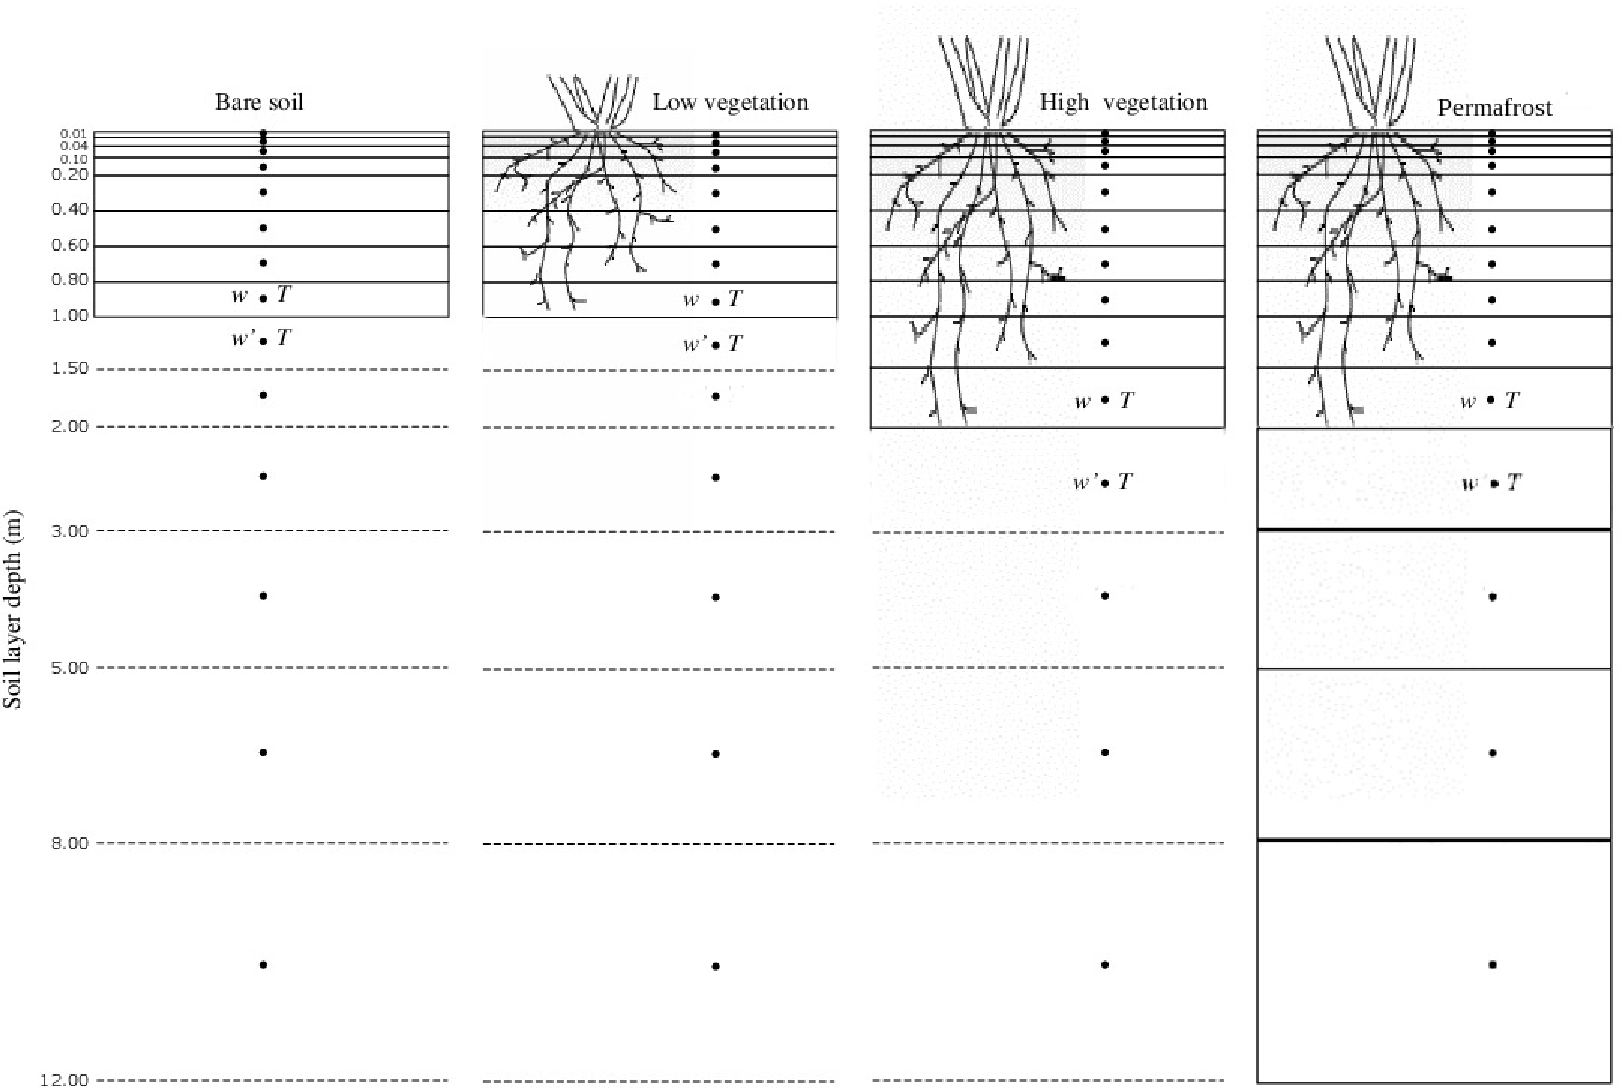
\includegraphics[angle=0, width=15cm]{\EPSDIR/isba-dif_water-thermal-grids.pdf}}
\caption{
The ISBA-DF soil grid configurations. Prognostic variable nodes (for
liquid water, $w_g$, soil ice, $w_{gf}$ and temperature, $T_g$) are located
at the center of each of the layers. There are 14 layers used for
thermal computations, and the same default 
grid thicknesses are used everywhere (note this can be modified by the
user). Hydrological grids are enclosed
by the solid black lines: thus the soil water prognostic equations do
not extend as deeply as the thermal computations except for areas/grid
cells with permafrost. See Decharme \etal (2013) for more details.
}
\label{fig:isba-dif_soil_grid}
\end{figure}
%%%%%%%%%%%%%%%%%%%%%%%%%%%%%%%%%%%%%%

Finally, the thicknesses of the current 14 layers have
been arranged to minimize numerical errors in solving
energy and water diffusion equations, especially in the first
meter of soil (Decharme \etal 2011). Note that the thermal
and/or hydrological lower boundary conditions of the soil,
as well as the thickness and the number of layers, can be
modulated by the user.

\paragraph{Numerical solution of the soil temperature equation}
%
Neglecting the phase transformation term,
Eq.~(\ref{teq}) can be written using an implicit time scheme as
%
\begin{equation}\label{teqcn}
{T_j}^{n}\,\,=\,\, {T_j}^{n-1} \,+\, 
\frac{\Delta t }{c_{g\,j}\,\Delta z_j}
\left[
\left(1-\varphi\right)
\left( {G_{j-1}}^{n-1} \,-\, {G_j}^{n-1} \right) +
\varphi
\left( {G_{j-1}}^{n} \,-\, {G_j}^{n} \right)
\right] 
\end{equation}
%
where $\varphi=1$ (backward difference) is currently used
for the soil temperature profile ($\varphi=1/2$ corresponds
to the Crank-Nicolson scheme).
Using either scheme,
the linear set of diffusion equations can be cast in tridiagonal
form and solved with relative ease. Although the Crank-Nicolson
scheme is more accurate (second order), the surface energy budget
equation is solved in ISBA using the backward difference scheme,
so for consistency this scheme is used to evaluate the diffusion term
in Eq.~(\ref{teq}).

The superscripts $n-1$ and $n$ represent the values
at the beginning and end of the time step, $\Delta t$, respectively.
The solution method is shown in Appendix B.
Once the new temperature profile has been determined, phase changes
are evaluated and the profile is updated. The phase change method
is described in section 4.

%=========================================================================================================
\subsubsection{Liquid Soil Water}
%=========================================================================================================
%
The vertical soil water flux from Eq.~(\ref{cont1}) is 
derived assuming soil water transfer arises due to
pressure gradients and a background drainage, and it is
expressed as
%
%%%%%%%%%%%%%%%%%%%%%%%%%%%%%%%%%%%%%%%%%
\beq\label{darcy}
F \,\,=\,\, -k\, \frac{\partial}{ \partial z} 
\left( \psi \,+\, z \right) 
\,-\, \frac{D_{\nu\psi}}{\rho_w}\frac{\partial \psi}{\partial z}
\eeq
%%%%%%%%%%%%%%%%%%%%%%%%%%%%%%%%%%%%%%%%%
%
where $F$ is the vertical soil water flux (${\rm m\,s^{-1}}$),
$k$ is the hydraulic conductivity (${\rm m\,s^{-1}}$),
$\psi$ is the soil matric potential (m),
%, $K_d$ 
%is an additonal linear background (low) drainage term (m s${-1}$),
and $z$ is the soil depth (m). 
The first term on the right hand side
of Eq.~\ref{darcy} represents Darcy's law for liquid
water transfer. The second term 
represents the water flux due to vapor transfer.
%The third is used to maintain a minimum 
%streamflow under dry conditions.
The isothermal vapor conductivity $D_{\nu\psi}$ 
(kg m$^{-2}$ s$^{-1}$) is a function of soil texture,
water content and temperature following Braud \etal (1993)\nocite{Braud1993-10-01},
except for some slight modifications due to the inclusion of
soil ice outlined here.

This representation of the fluxes results in the so-called
``mixed-form'' of the Richard's equation. It permits the
use of a heterogenous soil texture profile (by considering
the gradient of matric potential which is continuous as opposed to soil
water content which is not necessarily continuous when the soil
properties vary).

Finally, when soil ice is present, Eq.~\ref{darcy} is modified
as
%
%%%%%%%%%%%%%%%%%%%%%%%%%%%%%%%%%%%%%%%%%
\beq\label{darcy_frz}
F \,\,=\,\, -k\, \left(
\wp \, \frac{\partial\psi}{ \partial z} 
\,-\, z \right) 
\,-\, \frac{\wp\,D_{\nu\psi}}{\rho_w}\frac{\partial \psi}{\partial z}
\eeq
%%%%%%%%%%%%%%%%%%%%%%%%%%%%%%%%%%%%%%%%%
%
where the non-dimensional coefficient $\wp$ has been introduced 
which acts to limit
vertical diffusion in the presence of a freezing front
(see Eq.~\ref{iceimp}).

\paragraph{Flux parameterization}
%
The vertical soil water flux term [Eq.~(\ref{darcy})] 
can be expressed in more compact form as:
%
\begin{equation}\label{darcy2}
F \,\,=\,\, -\eta \, \frac{\partial \psi}{\partial z} \,-\, k
%- \zeta
\end{equation}
%
where $\eta$ (${\rm m^2\,s^{-1}}$)
represents the effective diffusion coefficient.
% and $\zeta$
%is the total drainage flux (m s$^{-1}$).
It is expressed as
%
%%%%%%%%%%%%%%%%%%%%%%%%%%%%%%%%%%%%%ù
\begin{equation}
\eta = \wp \, \left(k \,+\, \frac{D_{\nu\psi}}{\rho_w}\right) 
%\zeta &= k + K_d \cr
\end{equation}
%%%%%%%%%%%%%%%%%%%%%%%%%%%%%%%%%%%%%ù
%
The first term on the RHS of
Eq.~\ref{darcy2} is the diffusion term and usually
is positive (directed upward), the exceptions possibly being
during precipitation, snowmelt or perhaps soil thaw events.
The second term on the RHS of Eq.~(\ref{darcy2}) 
represents total drainage and is always directed (positive) downward.
During strong infiltration events (rainfall, snowmelt etc...)
generally $k$ dominates the (downward) water flux.
%
Note that if vapor diffusion is neglected and the soil is not frozen,
%and the linear drainage term (option) is negligible, 
the vertical flux
given by Eq.~(\ref{darcy})
collapses into the standard Darcy flux expression
for liquid water movement:
%
%%%%%%%%%%%%%%%%%%%%%%%%%%%%%%%%%%%%%%%%%%%%%%%%%%%%%%%%
\begin{equation}
\label{darcy3}
F \,\,=\,\, -k\, \frac{\partial }{\partial z} 
\left( \psi \,+\, z \right) 
\end{equation}
%%%%%%%%%%%%%%%%%%%%%%%%%%%%%%%%%%%%%%%%%%%%%%%%%%%%%%%%
%
%AABHERE

\subparagraph{Soil Freezing}
%
As a soil freezes, ice is assumed to become part
of the soil matrix thereby reducing the liquid water 
holding capacity of the soil. The degree of saturation
of the soil by liquid water is expressed 
%following Kowalczyk (1998) 
as
%
%
%%%%%%%%%%%%%%%%%%%%%%%%%%%%%%%%%%%%%%%%%%%%%%%%%%%%%%%%
\begin{equation}
\label{srl}
\Theta \,\,=\,\, \frac{w-w_i}{w_{sat}-w_i}
\,\,=\,\, \frac{w_l}{w_{sat\,l}}
\hskip.5in (0\,\leq\, \Theta \,\leq\, 1)
\end{equation}
%%%%%%%%%%%%%%%%%%%%%%%%%%%%%%%%%%%%%%%%%%%%%%%%%%%%%%%%
%
%
where $w_{sat\,l}$ represents the soil liquid water
holding capacity. The porosity is decreased in the presence of
soil ice as it is assumed ice becomes part of the soil matrix
(see Boone \etal (2000) for more information).

The hydraulic conductivity and soil water potential
are related to the liquid volumetric soil water content
through the relations (Clapp and Hornberger, 1978):
%
\beq\label{k}
 k \,\,=\,\,k_{sat}\,{\Theta}^{2b+3} 
\eeq
%
\beq\label{psi}
 \psi =\,\,\psi_{sat}\,{\Theta}^{-b} 
\eeq
%
where $b$ is an empirical parameter, $k_{sat}$ is the 
hydraulic conductivity at saturation, $\psi_{sat}$ is
the water potential at saturation and $w_{sat}$ is the soil
porosity. 
In recent years, several SVATs (eg. VISA: Yang and Niu, 2003\nocite{Yang2003})
have adopted the idea
that the saturated hydraulic conductivity decreases
exponentially with increasing soil depth (Beven and Kirby, 1979). 
This can be handled by ISBA-DF since Richard's equation
is expressed in mixed-form (i.e. a heterogeneous profile
of $k_{sat}$ can be specified).

Soil ice has the effect of decreasing the hydraulic
conductivity relative to a thawed soil
with the same total soil moisture.
The ice impedance coefficient is represented by
$\wp$. It is calculated following Johnsson and Lundin (1991):
%
\begin{equation}\label{iceimp}
\wp \,\,=\,\,{10}^{-a_\wp \,w_i/w}
\end{equation}
%
where the coefficient $a_\wp$ is currently assigned a value
of 6 proposed by Lundin (1990)\nocite{Lundin1990}. This coefficient prevents
an overestimation of the upward 
liquid water flux to the freezing front. Note that the model
is rather sensitive to this parameter, and a calibration might
be required to obtain optimal agreement with observations.
The dependence of $\wp$ on ice content ratio ($w_i/w$)
is shown in Fig.~\ref{iceimped}. 
Note that the effect of this 
coefficient is currently under investigation, and that alternate
formulations (such as dependence on soil temperature rather than
soil ice) will also be explored.

\begin{figure}[h]
		 \begin{center}
		 \psfig{figure=\EPSDIR/Eice.pdf,width=8cm}
		 \caption{The dependence on the water flux impedance factor ($\wp$)
on soil ice fraction ($w_i/w$) for various
values of $a_\wp$ (denoted as ``Eice'' in the figure). 
This coefficient is multiplied by the
vertical soil water flux, and as such can strongly modulate
vertical flow of liquid water and subsequent
freezing.}
		 \label{iceimped}
		 \end{center}
\end{figure}



\subparagraph{Vapor diffusion}
%
The isothermal vapor conductivity can be expressed as
%
\begin{equation}\label{vapdif}
D_{\nu\psi} \,\,=\,\,
D_\nu \, \frac{\partial\rho_\nu}{\partial\psi}
\end{equation}
%
where $\rho_\nu$ represents the water vapor density in the air-filled pore 
space of the soil, and $D_\nu$ represents an effective molecular
diffusivity (Milly (1982)\nocite{Milly1982}). It can be written following
Braud \etal (1993) as
%
\begin{equation}\label{vapmoldif}
D_\nu \,\,=\,\,
D_{\nu a} \,\alpha_\nu \, f_{\nu a}
\frac{p}{ \left(p-p_\nu\right)}
\end{equation}
%
where the tortuosity is $\alpha_\nu = 0.66$,
and the atmospheric and soil vapor pressures
are represented by $p$ and $p_\nu$, respectively.
The function $f_{\nu a}$ is defined as
%
%%%%%%%%%%%%%%%%%%%%%%%%%%%%%%
\[ f_{\nu a} = \left\{ \begin{array}{ll}
\left[w_{sat} - \left(w_l+w_i \right)\right]
\left[1 \,+\, 
{\left(w_l+w_i \right)/
\left(w_{sat}-w_k \right)}
\right]
& \mbox{if $\left(w > w_k\right)$} \\
%
w_{sat} & \mbox{if $\left(w \leq w_k \right)$}
\end{array} 
\right. \] 
%%%%%%%%%%%%%%%%%%%%%%%%%%%%%%
%
where $w_k$ is a parameter which defines the point corresponding to
the loss of continuity of the liquid phase in the soil pores 
(0.05 m$^3$ m$^{-3}$ for the current study). The function
$f_{\nu a}$ is related to the available pore space for vapor, or volumetric 
air content ($w_{sat}-w_l-w_i$).
The molecular diffusivity coefficient for water
vapor is given as
%
%
%%%%%%%%%%%%%%%%%%%%%%%%%%%%%%%%%%%%%%%%%%%%%%%%%%%%%%%%
\begin{equation}
\label{moldify}
D_{\nu a} \,\,=\,\,
c_\nu \, \left(\frac{p_0}{ p}\right)
{\left(\frac{T }{ T_f}\right)}^{n_\nu}
\end{equation}
%%%%%%%%%%%%%%%%%%%%%%%%%%%%%%%%%%%%%%%%%%%%%%%%%%%%%%%%
%
%
where $c_\nu = 2.17 \times {10}^{-5}$ m$^2$ s$^{-1}$,
$n_\nu = 1.88$, and $p_0 = {10}^6$ Pa. It is assumed that the soil
water vapor is in equilibrium with the liquid, and that
the air is saturated with respect to the 
ice present in the soil
so that the vapor density can be expressed as
%
%
%%%%%%%%%%%%%%%%%%%%%%%%%%%%%%%%%%%%%%%%%%%%%%%%%%%%%%%%
\begin{equation}
\label{vapden}
\rho_\nu \,\,=\,\,
\rho_{\nu\,sat}(T)
\chi_{sat} \, h_\nu
\,+\,
\left( 1-\chi_{sat}\right) \rho_{\nu\,sat\,i}{\rm min}(T,T_f)
\end{equation}
%%%%%%%%%%%%%%%%%%%%%%%%%%%%%%%%%%%%%%%%%%%%%%%%%%%%%%%%
%
%
where the humidity is given by
%
%
%%%%%%%%%%%%%%%%%%%%%%%%%%%%%%%%%%%%%%%%%%%%%%%%%%%%%%%%
\begin{equation}
\label{vaphum}
h_\nu \,\,=\,\,
{\rm exp}\left( \frac{\psi\,g}{ R_\nu \,T}\right)
\end{equation}
%%%%%%%%%%%%%%%%%%%%%%%%%%%%%%%%%%%%%%%%%%%%%%%%%%%%%%%%
%
%
The soil ice factor is defined as
%
%%%%%%%%%%%%%%%%%%%%%%%%%%%%%%%%%%%%%%%%%%%%%%%%%%%%%%%%
\begin{equation}
\label{chisat}
\chi_{sat} = \left(w_{sat}-w_i\right)/w_{sat}
\end{equation}
%%%%%%%%%%%%%%%%%%%%%%%%%%%%%%%%%%%%%%%%%%%%%%%%%%%%%%%%
%
% 
Taking the derivative of $\rho_\nu$ with respect to $\psi$
and substituting the resulting expression and
Eq.~(\ref{vapmoldif}) into Eq.~(\ref{vapdif}) 
using the ideal gas law for water
vapor results in
%
%
%%%%%%%%%%%%%%%%%%%%%%%%%%%%%%%%%%%%%%%%%%%%%%%%%%%%%%%%
\begin{equation}
\label{vapdif2}
D_{\nu\psi} \,\,=\,\,
\frac{\alpha_\nu \,p }{ \left( p-p_\nu\right)}
\frac{D_{\nu a}\,f_{\nu a}\,\chi_{sat} \,g \, p_{\nu\,sat} \,h_\nu
}{ {\left(R_\nu \,T\right)}^2}
\end{equation}
%%%%%%%%%%%%%%%%%%%%%%%%%%%%%%%%%%%%%%%%%%%%%%%%%%%%%%%%
%

\begin{figure}[h]
		 \begin{center}
		 \psfig{figure=\EPSDIR/vapdif.pdf,width=8cm}
		 \caption{Soil vapor diffusion coefficient ($d_\nu$) for four soil
textures assuming constant soil temperature
and pressure.}
		 \label{vapdiffig}
		 \end{center}
\end{figure}

The diffusion coefficient ($d_\nu$) is
shown in Fig.~(\ref{vapdiffig}) 
for four soil textures 
over the entire range of soil wetness
($w_l/w_{sat}$) assuming a constant
temperature and pressure of 300 K and 101325 Pa,
respectively. It is largest, in general, for the
most coarse textured soils approximately
at or below the soil permanent wilting point value.
A comparison between the vapor diffusion and
the hydraulic conductivity are shown in
Fig.~(\ref{vapdiffig2}). This shows that vapor diffusion
comprises the most significant contribution to 
the net diffusion process over a soil water range
around the wilting point. In the ISBA force-restore method, this vapor
phase transfer is parameterized within the coefficient $C_1$ for dry soil
(Braud \etal (1993) and Giordani (1996)\nocite{Giordani1996}).
%
As a final note, strictly speaking, vapor diffusion involves latent
heating effects which couples the mass and heat eqiuations very
tightly over a certain range of temperature and soil moisture. 
But currently in ISBA, the effect of vapor diffusion is simply modeled
by increasing the effective diffusivity of liquid transfer as a first
order approach (thus, mass is conserved and energy is unchanged) since
historically, the goal was to maintain baresoil evaporation under dry
but sufficiently hot surface conditions. Future work could consist in adding
the latent heating effect.

\begin{figure}[h]
		 \begin{center}
		 \psfig{figure=\EPSDIR/vapdif2.pdf,width=8cm}
		 \caption{The total hydraulic conductivity contributions
from liquid water ($k$) and vapor ($D_{\nu\psi}$)
for three soil textures as a function of soil wetness.
The soil temperature and surface atmospheric pressure have constant
values of 285 K and 10$^5$ Pa, respectively.}
		 \label{vapdiffig2}
		 \end{center}
\end{figure}

%\subparagraph{Linear Drainage}
%
%ISBA is increasingly used in studies for which river hydrology is simulated.
%The standard Richard's equation poses a problem for dry conditions in
%that the observed constant minimum riverflow occuring during dry seasons
%is poorly simulated. The actual cause of such flows is most likely subterranian
%lakes, surface lakes, water table interactions, etc., which are all not currently 
%explicitly modeled by ISBA. The most simplistic fix to this problem is to
%impose a linear drainage term which can be calibrated based on observed minimum
%riverflows outside of periods of active precipitation or snowmelt.
%
%Etchevers \etal (2002)\nocite{Etchevers2002} calibrated such a parameter for the 3-layer ISBA
%Force-Restore approach and greatly improved discharge statistics for certain
%sub-basins within the Rhone basin in France. In this method, a drainage
%is calculated assuming the water content is at some small increment just
%above field capacity (thereby resulting in a steady, but relatively small
%drainage flux). Adapting this method into the current model results in
%
%%%%%%%%%%%%%%%%%%%%%%%%%%%%%%%%%%%%%%%%%%%%%%%%%%%%%%%%
%\begin{equation}
%K_d = k_{sat} {\left[\left(w_{fc} + w_{drain}\right)/w_{sat}\right]}^{2b+3} \times
%\Biggr\lbrace \frac{
%\left[{\rm min}\left(w_{fc},w_l\right)-w_{min}\right] 
%}{\left(w_{fc}-w_{min}\right)
%}\Biggr\rbrace
%\end{equation}
%%%%%%%%%%%%%%%%%%%%%%%%%%%%%%%%%%%%%%%%%%%%%%%%%%%%%%%%
%
%
%The term on the left of the multipication sign
%is constant in time.
%The rightmost term is a linear scaling term which reduces the constant
%drainage as the source soil layer dries out. The field capacity water
%content is given by $w_{fc}$. The $w_{drain}$ can be calibrated and is generally
%on the order of 0.001 m$^3$ m$^{-3}$, although it can vary by an order
%of magnitude. It is zero (therefore $K_d=0$) when this option is off
%(i.e. local scale studies etc.).

\paragraph{Layer averaging}
%
Integrating Eq.~(\ref{cont1})
downward into the soil to obtain the prognostic equation for
the layer-average volumetric liquid water content for each $j$ layer
gives
%
\beq\label{int_continuity}
\int_{-z_j}^{-z_{j-1}} 
\frac{\partial w_l}{ \partial t } dz \,\,=\,\,
-\int_{-z_j}^{-z_{j-1}} 
\frac{\partial F}{ \partial z} dz \,-\,
\int_{-z_j}^{-z_{j-1}} \left(S_l-\frac{\Phi}{ L_f\rho_w}\right) dz
\eeq
%
where
%
\beq\label{avgtheta}
w_{l\,j} \,\,=\,\, \frac{1}{ \Delta z_j} \int_{-z_j}^{-z_{j-1}}
w_l dz
\eeq
%
$w_{l\,j}$ is the layer averaged volumetric liquid water
content ($j=1,...,N$).

Carrying out the integration in Eq.~\ref{int_continuity} using 
Eq.~\ref{avgtheta} yields
%
%%%%%%%%%%%%%%%%%%%%%%%%%%%%%%%%%%%%%%%%%%%%%%%%%%%%%%%%
\begin{equation}
\label{avgcont}
\Delta z_j {\frac{w_{l\,j}}{\partial t}} \,\,=\,\,
F\Big\vert_{-z_j} \,-\, 
F\Big\vert_{-z_{j-1}} \,-\, Q_j \,-\,
{\frac{\Delta z_j\, \Phi_j}{L_f\rho_w}} 
\end{equation}
%%%%%%%%%%%%%%%%%%%%%%%%%%%%%%%%%%%%%%%%%%%%%%%%%%%%%%%%
%
%
where 
%
\beq\label{avgsinkQ}
Q_j \,\,=\,\, \Delta z_j\,S_j 
\eeq
%
is in kg m$^{-2}$ s${-1}$.
The flux across a model level ($z_j$) is written as
%
%%%%%%%%%%%%%%%%%%%%%%%%%%%%%%%%%%%%%%%%%%%%%%%
\begin{subequations}
\begin{align}
\label{waterflux}
F\Big\vert_{-z_j} \,\,=&\,\,
F_j \,\,=\,\,
{\overline\eta}_j \,
\left[ \frac{\psi_{j+1}-\psi_{j}}
{\left(\Delta z_j+\Delta z_{j+1} \right)/2}\right] 
\,-\,{\overline k}_j 
\\
\label{waterflux_b}
{\overline\eta}_j \,\,=&\,\, \wp_j \left( {\overline k}_j + 
\frac{{\overline D}_{\nu\psi,j}}{\rho_w} \right)
\end{align}
\end{subequations}
%%%%%%%%%%%%%%%%%%%%%%%%%%%%%%%%%%%%%%%%%%%%%%%
%
where ${\overline k}_j$ and ${\overline D}_{\nu\psi,j}$ 
(both in m s$^{-1}$) represent the geometric means over two
consecutive
nodes of the soil hydraulic conductivity
and isothermal vapor conductivity values, respectively.
The inter-facial hydraulic conductivity is defined as
%
%%%%%%%%%%%%%%%%%%%%%%%%%%%%%%%%%%%%%%%%%%%%%%%
\begin{equation}
\label{kinterp}
{\overline k}_j = \sqrt{k_j\left(\psi_j\right) 
\times k_{j+1}\left(\psi_{j+1}\right)}
\end{equation}
%%%%%%%%%%%%%%%%%%%%%%%%%%%%%%%%%%%%%%%%%%%%%%%
%
The choice of an appropriate intra-block approximation for unsaturated
hydraulic conductivity has been pointed out as critical in the
numerical solution of unsaturated flow by many studies.
As discussed in Decharme et al. (2011)/nocite{Decharme2011},
%(Haverkamp et al., 1977; 
%Haverkamp and Vauclin, 1979; 
%Hornung and Messing, 1983;
%Schnabel and Richie, 1984; 
%Warrick, 1991; 
%Zaidel and Russo, 1992; 
%Feng et al., 2007). 
many studies have demonstrated 
that the geometric mean generates little weighting error, improves the
simulated infiltration front, and is generally applicable in all
situations.

%AABHERE
 

% OLD ---------------------------------------------------------
% OLD psi interp
%
%${\tilde\psi}$ represents the so-called interfacial matric
%potential. It is calculated from
%%
%\beq\label{sinterp}
%{\tilde\psi}_{j} \,\,=\,\,
%\delta_{\psi\,j} \, \psi_{j} \,+\, (1-\delta_{\psi\,j})
%\psi_{leq\,j} 
%\eeq
%
%where the delta function $\delta_{\psi\,j}$ is
%defined as
%
%
%%%%%%%%%%%%%%%%%%%%%%%%%%%%%%
%\[ \delta_{\psi\,j} = \left\{ \begin{array}{ll}
%        1 & \mbox{if $\psi_{j} \geq \psi_{leq\,j}$}
%\\
%        0 & \mbox{if $\psi_{j} < \psi_{leq\,j}$}
%\end{array} 
%\right. \] 
%%%%%%%%%%%%%%%%%%%%%%%%%%%%%%
%
%hydrostatic equilibrium.
%It is calculated assuming that the total matric potential
%or head is constant from the layer interface ($z_j$)
%to the mid-point of the layer below
%(Noilhan and Planton (1989), Koster and 
%Suarez (1996)\nocite{Koster1996}): ${\partial\psi/\partial z}=-1$:
%
%%%%%%%%%%%%%%%%%%%%%%%%%%%%%%%%%%%%%%%%%%%%%%%%%%%%%%%%
%\begin{equation}
%\label{psieq}
%\psi_{leq\,j} \,\,=\,\, \psi_{j+1} \,-\,
%\left(\Delta z_j+\Delta z_{j+1}\right)/4 \,\,\,.
%\end{equation}
%%%%%%%%%%%%%%%%%%%%%%%%%%%%%%%%%%%%%%%%%%%%%%%%%%%%%%%%
%
%
%From Eq.~(\ref{sinterp}), diffusivity and conductivity
%are evaluated using the so-called upstream value of the matric potential,
%which is similar to the simple model proposed by Mahrt and 
%Pan (1984)\nocite{Mahrt1984},
%except that the equilibrium matric potential value is used in
%place of the lower layer matric potential (equivalently the
%volumetric water content in their case as they assumed a
%homogenous soil texture profile). As in Mahrt and Pan (1984),
%the upper layer matric potential (water content in their case)
%is used in the presence of a wetting front. Such an interpolation
%is needed due to the coarse nature of the vertical grid mesh typically
%used in SVATs intended for atmospheric models.
%
% OLD psi interp
% OLD ---------------------------------------------------------

A graphic representation of the interpolation method is
shown for two contiguous soil layers with different
textures (and therefore, different soil hydraulic 
properties) in Fig.~\ref{kint}. 

\begin{figure}[h]
		 \begin{center}
		 \psfig{figure=\EPSDIR/kint_anglais.pdf,width=10cm}
		 \caption{The interfacial hydraulic
                   conductivity. ${\overline k}_j$
represents the hydraulic conductivity centered at $z_j$, and
${\tilde\Delta} z_j = 
\left(\Delta z_{j} + \Delta z_{j+1}\right)/2$.}
		 \label{kint}
		 \end{center}
\end{figure}

%This method results in
%a better approximation of the soil water flux than 
%specifying that the flux from the mid-point of 
%layer $\Delta z_j$ to $z_j$ is equal to that from
%layer $z_j$ to the mid-point of layer $\Delta z_{j+1}$
%(as is used to derive the soil heat flux),
%as the diffusivity and conductivity are more consistent
%with the soil water gradient (Mahrt and Pan (1984)). 

\paragraph{Boundary Conditions}
%
\subparagraph{Lower Boundary}
%
The lower boundary condition is modeled as gravitational drainage
(vertical diffusion is neglected). The mean water content of the lowest
layer is used to evaluate the flux
so that from Eq.~(\ref{waterflux}) one can write
%
%%%%%%%%%%%%%%%%%%%%%%%%%%%%%%%%%%%%%%%%%%%%%%%%%%%%%%%%
\begin{equation}
\label{lowerwaterbc}
F_N \,\,=\,\, -k_N 
%F_N \,\,=\,\, -\zeta_N \,\,=\,\, -k_N 
%- K_d 
\end{equation}
%%%%%%%%%%%%%%%%%%%%%%%%%%%%%%%%%%%%%%%%%%%%%%%%%%%%%%%%
%
%
%Under moist conditions, $F_N \approx -k_N$,
%whereas for very dry conditions, it is possible
%that $K_d$ dominates the drainage (depending on the
%value specified for $K_d$).
%
The diffusion term
(i.e. capillary rise across the lower model boundary) 
can be significant, however, when the water table is near
$z_N$. An option exists for utilizing this information
using a simple expression consistent with the vertical flux
formulation used for the other model layers.
%, however
%it is currently not included in the current model
%release (as typically water table information is
%not available in atmospheric models).
%
In this case, $F_N$ is modified to be
%
%%%%%%%%%%%%%%%%%%%%%%%%%%%%%%%%%%%%%%%%%%%%%%%%%%%%%%%%
\begin{align}
\label{lowerwaterbcx}
F_N \,\,=&\,\, -k_N \left[
f_{wtd}
\left( \frac{\psi_{N}-\psi_{sat}}{\Delta z_{wtd}} + 1\right)
\,+\, \left(1- f_{wtd}\right)
\right]
\\
\label{lowerwaterbcxz}
\Delta z_{wtd} \,\,=&\,\,
{\rm min}\left( z_N,\,z_{wtd}\right) \,-\,
\left( z_N + z_{N-1}\right)/2
\end{align}
%%%%%%%%%%%%%%%%%%%%%%%%%%%%%%%%%%%%%%%%%%%%%%%%%%%%%%%%
%
where $f_{wtd}$ is the gird-cell fraction 
where capillary rise occurs. It
can be 1 at the local scale or depend on topography at larger
scales. Indeed, only a fraction of the grid cell corresponding to the
flat valleys and alluvial plains should be affected by water
capillary rises. This fraction must reflect the subgrid topographical
heterogeneity inside each grid cell, which can be significant, for
example, 
when considering the coarse resolution of the climate models. A
grid cell with steeper topography would be affected by upward
capillary fluxes over a small fraction of the grid cell, 
unlike those characterized by relatively 
flatter terrain. See 
Vergnes et al. (2014)\nocite{Vergnes2014} for more details.


\subparagraph{Upper Boundary}
%
The upper boundary condition represents infiltration.
%
By default, the soil infiltration $I$ is equal to the
potential (supply limited) infiltration rate, i.e. $I = R_t$. 
%where $R_t$
%(m s$^{−1}$) is the through-fall rate (sum of canopy drip, precipitation
%and snow-melt). 
This case is specially relevant for local scale
studies. 
The soil-water infiltration is put preferentially in the first layer. If
this first layer can not contain this amount of water, the remaining
is forced into the next layer and so forth (downward).

An Horton runoff option exists that computes the soil infiltration via
a Green and Ampt (1911) approach (Decharme et al. 2013)\nocite{decharme_ea_2013}. 
This approach, based on Darcy’s law, includes the hydrodynamic parameters
of the soil and determines the infiltration capacity of soil over the
time. It represents the soil infiltration as a wetting front in which
the hydraulic gradient is uniform. In ISBA-DF, the analytical form of the
Green-Ampt approach is used to determine the maximum amount of water
that infiltrates the soil to a depth close to 0.1 m (the thickness
generally used for relatively large time steps). 
The infiltration capacity, $I_c$
(kg m$^{-2}$ s$^{-1}$), is therefore parameterized as:
%
%%%%%%%%%%%%%%%%%%%%%%%%%%%%%%%%%%%%%%%%
\begin{equation}
\label{eq:infiltration_capacity}
%
I_c = \frac{\rho_w}{z_{nic}} \sum_{i=1}^{nic}
\left[
\wp_i \, k_{sat,i}
\left(
\frac{\psi_{sat}-\psi_{i}}{\Delta z_i} \,+\, 1
\right) \Delta z_i
\right]
\end{equation}
%%%%%%%%%%%%%%%%%%%%%%%%%%%%%%%%%%%%%%%%
%
where $z_{nic}$ (m) 
represents the depth of the layer $nic$ that is the nearest 0.1 m, and 
$\Delta z_i$ (m) is the thickness of each of the $i$ layers. 
Finally, the soil-water
infiltration in ISBA-DF can be computed by comparing this infiltration
capacity with the flux of water reaching the soil:
%
%%%%%%%%%%%%%%%%%%%%%%%%%%%%%%%%%%%%%%%%
\begin{equation}
\label{eq:upperwaterbc_nosubgrid}
%
I = {\rm min}\left(R_t, \, I_c \right)
\end{equation}
%%%%%%%%%%%%%%%%%%%%%%%%%%%%%%%%%%%%%%%%
%
All of the excess water (i.e. defined as $R_t-I$ when it is $>0$) 
is treated as a “Horton” surface runoff flux
whereas the soil infiltration is treated as a moisture source term.

For non-local scale applications, an alternate form of 
generating surface
runoff is needed. 
In this case, infiltration is computed as:
%
\beq\label{upperwaterbc}
I \,\,=\,\,{\rm min}(R_t-Q_r,\,I_c)
\eeq
%
It can also be computed via a variable infiltration capacity 
(VIC: Dumenil and Todoni, 1992)\nocite{Dumenil1992}
sub-grid surface runoff scheme
used in ISBA (Habets \etal 1999)\nocite{Habets1999}.
%
In this scheme,
$Q_r$ represents sub-grid surface runoff from saturated regions
within the computational unit/cell
(See Eq.s~\ref{eq:i_m_vic_model}-\ref{eq:a_vic_model} for the
theoretical background).
It is computed using a similar form as that for the Force-Restore
approach (Eq.s~\ref{qrc}-\ref{qrz}):
%
%%%%%%%%%%%%%%%%%%%%%%%%%%%%%%%%%%%%%%%%%%%%%%%%%%%%
\begin{subequations}
\begin{align}
\label{eq:qrc_df}
Q_{r\,{\rm crit}} \,\,=\,\, &
{\left[1 - {\left({\overline w}_r-{\overline w}_{c,min}\right)\over 
\left({\overline w}_{sat}-{\overline w}_{c,min}\right)}\right]}^{1/(1+{\rm b})}
\,-\,
{R_t \Delta t \over \rho_w z_r}
\left[{ 1\over
(1+{\rm b})\left({\overline w}_{sat}-{\overline w}_{c,min}\right)
}\right]
\\
\label{eq:qr_df}
Q_r \,\,=\,\, & R_t - {\rho_w z_r \over\Delta t}
\Biggr\lbrace
\left({\overline w}_{sat}-{\overline w}_r\right)-
\left({\overline w}_{sat}-{\overline w}_{c,min}\right) 
{\left[{\rm max}\left(0,\,Q_{r\,{\rm crit}}\right)\right]}^{1+{\rm b}}
\Biggr\rbrace
\end{align}
\end{subequations}
%%%%%%%%%%%%%%%%%%%%%%%%%%%%%%%%%%%%%%%%%%%%%%%%%%%%
%
with the constraints (as in Eq.~\ref{qrz}, but using a layer averaged
$w_{c,min}$):
%
%%%%%%%%%%%%%%%%%%%%%%%%%%%%%%%%%%%%%%%%%%%%%%%%%%%%%%%%
\begin{equation}
\label{eq:qrz_df}
Q_r \,\,=\,\, 0
\hskip.5in
{\rm if}\hskip.2in
\left(Q_r < 0 \right) 
\hskip.2in {\rm or}\hskip.2in 
\left({\overline w}_r \leq {\overline w}_{c,min}\right) 
\end{equation}
%%%%%%%%%%%%%%%%%%%%%%%%%%%%%%%%%%%%%%%%%%%%%%%%%%%%%%%%
%
%where $R_t$
%(m s$^{−1}$) is the through-fall rate (sum of canopy drip, precipitation
%and snow-melt). 
%${\overline w}_r$ represents the average total water
%
Note that currently, $w_{c,min}=w_{wilt}$ by default until further
studies can be done.
$Q_r$ is evaluated using the average total soil moisture, ${\overline w}_r$,
integrated from the surface down
to a characteristic depth, $z_r$. It is defined as
%
%%%%%%%%%%%%%%%%%%%%%%%%%%%%%%%%%%%%%%%%%%%%%%%%%%%%%%%%
\begin{equation}
\label{eq:water_content_avg_dif_vic}
{\overline w}_r = 
{\frac
{\left(\sum_{j=1}^{N_r} \Delta z_j \, w_j \right) + 
w_{N_r+1}{\rm max}\left(0,\,z_r-z_{N_r}\right)} 
{\left(\sum_{j=1}^{N_r} \Delta z_j \right) + 
{\rm max}\left( 0,\,z_r-z_{N_r}\right)}
}
\hskip.5in
\left(z_r \leq z_N\right)
\end{equation}
%%%%%%%%%%%%%%%%%%%%%%%%%%%%%%%%%%%%%%%%%%%%%%%%%%%%%%%%
%
where $N_r$ is the total number of soil layers for which
$z_r \geq z_j$ (i.e. the depth is greater than or equal to
the lower boundary of the
soil layer $j$). Note that the porosity and wilting point volumetric water
contents are also averaged over $z_r$ using the same operator.
This depth should be at least several tens of centimeters 
thick (Liang \etal 1996).

It should also be noted that several authors use a form
of Darcy's law assuming the soil right at the surface
is saturated as the maximum potential infiltration rate
(Mahrt and Pan, 1984\nocite{Mahrt1984}; 
Abramopoulos \etal 1988\nocite{Abramopoulos1988}).
This, however, has a very minimal impact on the infiltration
(compared to the above equations) for the time and space scales
considered in typical ISBA applications, and the linearization
of such a term can pose some numerical problems (the linearized
surface flux can actually exceed the amount of water available
for infiltration under some rare circumstances). 
%For these two
%reasons, Eq.~(\ref{infilt}) is used currently in ISBA.

\paragraph{Solution method}
%
The equation for liquid water transfer is
solved using:
%
%%%%%%%%%%%%%%%%%%%%%%%%%%%%%%%%%%%%%%%%%%%%%%%%%%%%%%%%
\begin{equation}
\label{watercn}
\varrho_j
({w_{l\,j}}^{n}-{w_{l\,j}}^{n-1}) \,\,=\,\,
\left(1-\varphi\right)
\left({F_j}^{n-1} \,-\,{F_{j-1}}^{n-1} \right)
\,+\, 
\varphi
\left( {F_j}^{n} \,-\,{F_{j-1}}^{n}\right) 
\,-\, {Q_j}^n
\end{equation}
%%%%%%%%%%%%%%%%%%%%%%%%%%%%%%%%%%%%%%%%%%%%%%%%%%%%%%%%
%
where $\varrho_j=\Delta z_j/\Delta t$, and 
$n$ indicates the value at the end of the time
step, $\Delta t$. 
The Crank-Nicolson time scheme is currently used to integrate
the equations in time (i.e., $\varphi=1/2$).
The flux terms can be linearized
or an iterative solution method can be used.
The linearization method is obviously more attractive for
numerical weather prediction applications as it consumes
less CPUs, and for this method,
an uppermost layer of several cm thickness can safely
be used for typical GCM (upper limit for $\Delta t$)
time steps (Bonan, 1996\nocite{Bonan1996}). 
Note that updates in mass owing to phase
changes ($\Phi$) are evaluated in a subsequent computation 
(see section 4).

\paragraph{Soil moisture sink term}
%
The sink term is composed of soil water 
losses/gains due to evapotranspiration/condensation
and gains due to lateral inflow or so-called soil
water excess. The production/reduction of soil ice
decreases/increases the liquid soil water content
while leaving the total soil water content unchanged.

\subparagraph{Evapotranspiration}
%
Bare soil evaporation, $E_g$, is extracted from
the uppermost soil layer only. Transpiration, $E_{tr}$,
can be extracted from multiple layers. A normalized root-zone
fraction is specified for each soil layer, and is zero
for layers below the root zone. 
Normalized transpiration weights are
then calculated based on the specified vertical root zone fraction and the
thickness of each model soil layer:
%
%%%%%%%%%%%%%%%%%%%%%%%%%%%%%%%%%%%%%%%%%%%%%%%%%%%%%%%%
\begin{equation}
\label{etrwght}
\xi_j \,\,=\,\, {\Upsilon_j \, \Delta z_j \over
\sum_{j=1}^N \Upsilon_j \, \Delta z_j}
\hskip.5in
(0 \,\leq\, \xi_j \,\leq\, 1)
\end{equation}
%%%%%%%%%%%%%%%%%%%%%%%%%%%%%%%%%%%%%%%%%%%%%%%%%%%%%%%%
%
%
where $\xi_j$ represents the transpiration weight.
Note that $\sum_{j=1}^N \xi_j = 1$ unless there are
no roots, in which case $\xi_j = 0$.
$\Upsilon_j$ represents the root fraction:
%
%%%%%%%%%%%%%%%%%%%%%%%%%%%%%%%%%%%%%%%%%%%%%%%%%%%%%%%%
\begin{equation}
\sum_j^N \Upsilon_j \,\,=\,\, 1 \,\,\,.
\end{equation}
%%%%%%%%%%%%%%%%%%%%%%%%%%%%%%%%%%%%%%%%%%%%%%%%%%%%%%%%
%
%
This parameter
is not well known for many regions and transpiration from SVAT
models can be highly sensitive to the vertical root zone distribution
(Desborough (1997)\nocite{Desborough1997}): this study suggests the use of a uniform distribution.
A uniform root zone distribution can be specified by
setting $\Upsilon_j$ constant within the root zone soil layer(s),
or a simple exponential function dependent on plant cover
can be specified (Jackson \etal (1996)\nocite{Jackson1996}).
%
In ISBA, the effect of water stress on transpiration
is modeled using a normalized soil moisture factor
(Noilhan and Planton, 1989; Calvet \etal 1998\nocite{Calvet1998a}):
%
%%%%%%%%%%%%%%%%%%%%%%%%%%%%%%%%%%%%%%%%%%%%%%%%%%%%%
\beq\label{normtheta}
%
%w_{n\,j} \,\,=\,\,
%{w_{l\,j}-\chi_{sat\,j} w_{wilt\,j}\over
%\chi_{sat\,j}\left(w_{fc\,j}-w_{wilt\,j}\right)}
%\hskip.5in
%(\epsilon \,\leq\, w_{n\,j} \,\leq\, 1)
%
w_{n\,j} \,\,=\,\,
\frac{w_{l\,j}-w_{wilt\,j}}
{\left(w_{fc\,j}-w_{wilt\,j}\right)}
\hskip.5in
\left(\epsilon \,\leq\, w_{n\,j} \,\leq\, 1 \right)
%
\eeq
%%%%%%%%%%%%%%%%%%%%%%%%%%%%%%%%%%%%%%%%%%%%%%%%%%%%%
%
where $w_{wilt}$ is the wilting point volumetric 
water content,
and $\epsilon$ is a small numerical
value ($\approx {10}^{-3}$ ). 
%The coefficient $\chi_{sat}$ is related to the reduction in
%layer-average porosity due to the inclusion of
%soil ice [Eq.~(\ref{chisat})].
%
From Eq.~(\ref{normtheta}),
soil ice in the root zone can hinder plant evaporation
even if atmospheric conditions are conducive to transpiration
and the total soil water content is above field capacity
since freezing produces an effective soil drying (reducing the liquid part).

The factor in Eq.~(\ref{normtheta})
is applied to the stomatal conductance so that transpiration
can proceed at an unstressed rate relative the soil water 
for moisture values above field capacity,
and is negligible for soils drier than wilting point.
The layer-averaged
water stress factor, which is applied to the net transpiration,
is calculated as Pan and Mahrt (1987)\nocite{Pan1987}
%
%%%%%%%%%%%%%%%%%%%%%%%%%%%%%%%%%%%%%%%%%%%%%%%%%%%%%%%%
\begin{equation}
\label{F2}
{\overline w}_n \,\,=\,\,
\sum_{j=1}^N \xi_j \,w_{n\,j} 
\end{equation}
%%%%%%%%%%%%%%%%%%%%%%%%%%%%%%%%%%%%%%%%%%%%%%%%%%%%%%%%
%
%
The above coefficients are simply used to partition the
transpiration among the various root-zone soil layers.

\subparagraph{Soil moisture excess}
%
When the increase over a given time period
in observed total soil water content 
exceeds that of precipitation less evapotranspiration,
a laterally induced source (negative sink) is assumed to
occur (Calvet \etal (1998)\nocite{Calvet1998}).
This can be due to lateral inflow of water (most likely) or
capillary rise from below the observation depth.
Since vertical diffusion across the base of the model is
assumed to be negligible, this source is parameterized as
lateral inflow. The vertical distribution is assumed to be
linear down to the depth of the soil moisture observations:
%
%
%%%%%%%%%%%%%%%%%%%%%%%%%%%%%%%%%%%%%%%%%%%%%%%%%%%%%%%%
\begin{equation}
\label{xswght}
\upsilon_j \,\,=\,\, {\delta_{\upsilon\,j} \Delta z_j \over
\sum_{j=1}^N \delta_{\upsilon\,j} \Delta z_j}
\end{equation}
%%%%%%%%%%%%%%%%%%%%%%%%%%%%%%%%%%%%%%%%%%%%%%%%%%%%%%%%
%
%
where $\upsilon_j$ represents the normalized soil water
excess coefficient, and $\delta_{\upsilon\,j}$ is a delta
function which is either 1 or 0 depending on whether or not
excess inflow is occurring in layer $j$. For applications where
soil moisture excess is not available, this source is set to zero.

\subparagraph{Liquid water sink}
%
The external soil water source/sink term 
[Eq.~(\ref{avgsinkQ})] is expressed as
%
%
%%%%%%%%%%%%%%%%%%%%%%%%%%%%%%%%%%%%%%%%%%%%%%%%%%%%%%%%
\begin{equation}
\label{netsink}
Q_j \,\,=\,\, 
%(1-\delta_{g\,j})
\,\xi_j \left({w_{n\,j}\over {\overline w}_n}\right)\,E_{tr} \,+\, 
\delta_{g\,j} \,E_{g\,L}
\,-\,\upsilon_j \,Xs 
\,\,\, .
\end{equation}
%%%%%%%%%%%%%%%%%%%%%%%%%%%%%%%%%%%%%%%%%%%%%%%%%%%%%%%%
%
%
$Xs$ represents the soil water excess (lateral
inflow). $E_{g\,L}$ is the evaporation from the bare soil
surface (uppermost layer),
and $\delta_{g\,j}$ is a delta function which
is unity only the uppermost soil layer
($\delta_{g\,1}=1$), and is zero
for all the other soil layers. The uppermost layer is prescribed to
be thin in order to capture the daily cycle in bare-soil evaporation.
The root zone fraction in this layer, $\Upsilon_1$, is usually set to zero.
The transpiration,
bare-soil evaporation and water excess terms are in
units of ${\rm kg \,\,m^{-2}\,s^{-1}}$. 

%\paragraph{Total latent heat flux}
%%
%Evaporation of liquid water in the soil
%and sublimation of soil ice are calculated based on
%the fraction of soil ice in the uppermost layer
%defined as $w_{i\,1}/w_1$. The total latent heat
%flux (W ${\rm m^{-2}}$) is then
%%
%$$ LE \,\,=\,\,L_f E_v \,+\, L_f E_{g\,L} \,+\, L_s E_{g\,I} \,\,\,,$$
%%
%where $L_s$ is the latent heat of sublimation (2834500 J ${\rm {kg}^{-1}}$).


%=========================================================================================================
\subsubsection{Soil water phase changes: freeze-thaw}
\label{sec:isba_soil_ice}
%=========================================================================================================
%
Soil ice [Eq.~(\ref{ice})] increases when there
is energy available for
ice production, while decreases are due to melting
and sublimation.
In order to avoid a more computationally intensive iterative 
solution procedure [between Eq.s~(\ref{tdifsn})-(\ref{ice})],
the soil temperature is first calculated using Eq.~(\ref{teqcn}),
then the phase change term ($\Phi_j$) is evaluated.
The temperature for a given layer
at time $n$ will then be adjusted at the end of the time
step such that ${T_j}^{n}\,\rightarrow\,T_f$ if melting
or freezing occurs (where $T_f$ is the freezing point temperature).

The method presented in Boone \etal (2000) and in Boone (2000)
for ISBA-DF has been modified owing to research involving
PILPS-2e (Bowling \etal (2003)\nocite{Bowling2003}) with
ISBA (Habets \etal 2002). In original test
simulations involving ISBA-DF using the PILPS-2e experimental design
and forcing, it was found that nearly all of the near surface
water froze, and this caused some unrealistic conditions
(although no observations are available to verify this).
Boone \etal (2000) treated NWP-time-scale events, and soil
freezing was not as extensive as in the PILPS-2e domain.
Thus, it was decided to adopt an approach which 
determines a maximum liquid water content as a function
of temperature using the Gibbs free energy method.
See for example Cox \etal (1999)\nocite{Cox1999},
Cherkauer and Lettenmaier (1999)\nocite{Cherkauer1999}
and Koren \etal (1999)\nocite{Koren1999}
for examples of this method used in SVATs. Many examples exist
in soil-science literature: see Boone (2000) for references.
The main difference between this method and the one presented
in Boone \etal (2000) is that 
not all of the available liquid water is frozen.
The method outlined herein represents a near seamless model
change in that it does not augment CPU's significantly,
and it requires no additional parameters.
It has been documented by Decharme \etal (2016).

The relation between the soil water potential and
temperature for sub-freezing conditions is
from Fuchs \etal (1978)\nocite{fuchs1978}:
%
%
%%%%%%%%%%%%%%%%%%%%%%%%%%%%%%%%%%%%%%%%%%%%%%%%%%%%%%%%
\begin{equation}
\label{eq:soil_ice_potential}
\psi^\ast = \frac{L_f \left( T - T_f\right)}{g\,T} 
\end{equation}
%%%%%%%%%%%%%%%%%%%%%%%%%%%%%%%%%%%%%%%%%%%%%%%%%%%%%%%%
%
The potential $\psi^\ast$ can be substituted
in the expression for the soil matric potential 
in order to obtain the maximum unfrozen (liquid) water content
at a given soil temperature, $T$.
Currently for ISBA, this is the Brooks and Corey (1966)\nocite{Brooks1966}
model as modified by Clapp and Hornberger (1978), so that
%
%%%%%%%%%%%%%%%%%%%%%%%%%%%%%%%%%%%%%%%%%%%%%%%%%%%%%%%%
\begin{equation}
w_{l\,{\rm max}} = w_{\rm sat} 
{\left(\psi^\ast\over \psi_{\rm sat}\right)}^{-1/b} 
\end{equation}
%%%%%%%%%%%%%%%%%%%%%%%%%%%%%%%%%%%%%%%%%%%%%%%%%%%%%%%%
%
%
During phase changes, the total soil water content
($w = w_l + w_i$) for each soil layer is conserved,
so that, for example, as a soil freezes, the liquid water
content will decrease owing to a corresponding increase
in soil ice content ($w_i$). This concept can be used 
to establish the maximum temperature at which soil
ice is present (again using the Gibbs free energy concept)
as
%
%%%%%%%%%%%%%%%%%%%%%%%%%%%%%%%%%%%%%%%%%%%%%%%%%%%%%%%%
\begin{equation}
T_{\rm max} = {L_f\,T_f \over \left( L_f - g \,\psi\right)} 
\end{equation}
%%%%%%%%%%%%%%%%%%%%%%%%%%%%%%%%%%%%%%%%%%%%%%%%%%%%%%%%
%
where the soil liquid water potential is defined 
as a function of the liquid water content using 
the relationship from Clapp and Hornberger (1978) [Eq.~(\ref{psi})].
The maximum unfrozen fraction
($w_{l\,{\rm max}}/w_{\rm sat}$) 
and $w_{l\,{\rm max}}$ as a function of temperature depression
are shown in Fig.~(\ref{wunfrz}).
for three soil textures. Note that a larger percentage of liquid water
can freeze for more coarse textured soils and that relatively dry
soils might have very cold temperatures before any freezing takes place.

\begin{figure}[h]
		 \begin{center}
		 \psfig{figure=\EPSDIR/soilicet.pdf,width=8cm}
		 \caption{The maximum unfrozen fraction
($w_{l\,{\rm max}}/w_{\rm sat}$) 
and $w_{l\,{\rm max}}$ as a function of temperature depression
for three soil textures. The corresponding porosity values ($w_{sat}$)
are shown in the right panel (thick horizontal lines) as a reference.}
		 \label{wunfrz}
		 \end{center}
\end{figure}

The phase change term is parameterized in a manner similar to that presented
in Boone (2000), Boone \etal (2000) and Giard and Bazile (2000),
but with the available thermal energy
evaluated using the difference $T_{\rm max} - T$ as opposed
to $T_f - T$, and the available liquid water for freezing being
defined using $w_l - w_{l\,{\rm max}}$ as opposed to
$w_l - w_{l\,{\rm min}}$. The freezing and melting terms
are, respectively:
%
\begin{eqnarray}
\Phi_{f\,j} = & {\rm min}
\left[
K_s \epsilon_f {\rm max}
\left( 0,\, T_{{\rm max}\,j}-T_j\right) c_i, \,\,
L_f \rho_w 
{\rm max}\left(0,\, w_{l\,j}-w_{l\,{\rm max}\,j}\right)
\right] /\tau_i
\cr
\Phi_{m\,j} = & {\rm min}
\left[K_s \epsilon_m {\rm max}
\left( 0,\, T_j-T_{{\rm max}\,j}\right) c_i, \,\,
L_f \rho_w w_{i\,j} \right]/\tau_i
\cr
\end{eqnarray}
%
where $c_i$ is the heat capacity of ice 
(1.883 ${\rm \times {10}^6 \,J\, K^{-1}\,m^{-3}}$).
A parameter which represents the characteristic time
scale for phase changes is represented by $\tau_i$
(Giard and Bazile, 2000). It
can be determined through calibration,
possibly (eventually) be related to soil texture.
A constant value of 3300 s$^{-1}$ is currently used.

The expressions for the phase change efficiencies ($\epsilon_f$ and $\epsilon_m$) 
are parameterized as functions of
liquid soil water for freezing and soil ice for
melting (similar to the method
used by Cogley \etal (1990)\nocite{Cogley1990} and Pitman \etal (1991)\nocite{Pitman1991}:
%
%
%%%%%%%%%%%%%%%%%%%%%%%%%%%%%%
\[ \epsilon_j = \left\{ \begin{array}{ll}
    w_{l\,j} /\left(w_{sat}-w_{i\,j}\right)
& \mbox{if $\left(T_j \,\leq\, T_f\right)$}
\\
w_{i\,j}/\left(w_{sat}-w_{\rm min}\right)
& \mbox{if $\left(T_j > T_f\right)$}
\end{array} 
\right. \] 
%%%%%%%%%%%%%%%%%%%%%%%%%%%%%%
%
%
The principle of using such coefficients is that 
it is assumed that when the grid box average liquid
soil moisture is relatively large, more energy is used
for freezing the soil compared to a more dry average soil
with the same available energy (for freezing). 
It is also a rudimentary method for modeling sub-grid freezing effects.
The same basic idea holds for soil ice melting.

The surface insulation
coefficient, $K_s$, is modeled following Giard and Bazile (2000) and
is written (here in non-dimensional form) as
%
%%%%%%%%%%%%%%%%%%%%%%%%%%%%%%%%%%%%%%%%%%%%%%%%%%%%%%%%
\begin{equation}
K_s = \left(1 - {veg\over K_2}\right)
\left(1 - {LAI\over K_3}\right)
\hskip.2in
\left(0 < K_s \leq 1 \right)
\end{equation}
%%%%%%%%%%%%%%%%%%%%%%%%%%%%%%%%%%%%%%%%%%%%%%%%%%%%%%%%
%
%
where the values from Giard and Bazile (2000) are used:
$K_2 = 5$ and $K_3 = 30$ m$^2$ m$^{-2}$.
%
For relatively dense vegetation covers (i.e., large $LAI$ and $veg$),
more energy is used to heat or cool the vegetation while less
is used to freeze/thaw the soil water/ice (compared to a surface
with less vegetation).

The total phase change
is then simply expressed as the difference between the freezing and melting components,
although note that one or the other is always zero:
%
%%%%%%%%%%%%%%%%%%%%%%%%%%%%%%%%%%%%%%%%%%%%%%%%%%%%%%%%
\begin{equation}
\Phi_j = \Phi_{f\,j} - \Phi_{m\,j}
\end{equation}
%%%%%%%%%%%%%%%%%%%%%%%%%%%%%%%%%%%%%%%%%%%%%%%%%%%%%%%%
%
%
Using the above model, the phase changes tend to follow the
so-called soil specific freezing characteristic curve
from Fuchs \etal (1978), although there can be considerable scatter
about this line owing to $\epsilon < 1$ and $K_s < 1$,
and ice can be present at significantly above-freezing layer-average temperatures.
In the limit as $\epsilon$ and $K_s$ become unity, the scatter
is greatly reduced, and the presence of ice at above-freezing
temperatures is also greatly reduced.

An example of the application of the above model to
a cold climate is shown in
Fig.~(\ref{fcurv}). The forcing and parameters
are from Goose Bay, Canada (Ross Brown, personal communication).
The relationship between simulated 
soil temperature and liquid water content for all 5 soil layers
using the model as presented herein is shown in the upper panel, and the
relationship for
which $\epsilon$ and $K_s$ have been set to zero
is shown in the lower panel. Each point represents at value
at a 30-minute time step for which either $T_j \leq T_f$
or $w_{i\,j} \geq 0.001$ m$^3$ m$^{-3}$.

\begin{figure}[h]
		 \begin{center}
		 \psfig{figure=\EPSDIR/fcurve2.pdf,width=8cm}
		 \caption{The simulated unfrozen liquid water fraction ($w_l/\left(w_i+w_l\right)$)
as a function of temperature depression ($T_f-T$) for five soil
model layers. The forcing are from Goose Bay, Canada.
The parameters $\epsilon$ and $K_s$ 
have been set to one in the lower panel.}
		 \label{fcurv}
		 \end{center}
\end{figure}

Soil ice and the overall soil water content are decreased
due to sublimation. This term is expressed as
%
%%%%%%%%%%%%%%%%%%%%%%%%%%%%%%%%%%%%%%%%%%%%%%%%%%%%%%%%
\begin{equation}
\label{sublim}
S_i \,\,=\,\, \Delta z_1 \, E_{g\,I} \,\,\,
\,\,\,, 
\end{equation}
%%%%%%%%%%%%%%%%%%%%%%%%%%%%%%%%%%%%%%%%%%%%%%%%%%%%%%%%
%
%
where $E_{g\,I}$ represents the liquid water equivalent loss
of soil ice from the bare soil (uppermost) model layer 
(kg m$^{-2}$ s$^{-1}$). 

The temperature and soil water profiles are updated
at the end of the time step, $\Delta t$, using the
calculated phase change term
together with:
%
%%%%%%%%%%%%%%%%%%%%%%%%%%%%%%%%%%%%%%%%%%%%%
\begin{align}
\label{tdifsni}
{T_j}^{n\prime}\,\,&=\,\, 
{T_j}^{n} + {\Delta t\,\Phi_j\over c_{h\,j}}
\\
%
\label{conti}
{w_{L\,j}}^{n\prime} \,\,&=\,\, 
{w_{L\,j}}^{n} - {\Delta t\,\Phi_j\over L_f \rho_w}
\\
%
\label{icei}
{w_{I\,j}}^{n\prime} \,\,&=\,\, 
{w_{I\,j}}^{n} + 
{\Delta t\,\Phi_j\over L_f \rho_w}
%
\end{align}
%%%%%%%%%%%%%%%%%%%%%%%%%%%%%%%%%%%%%%%%%%%%%%%%%
%
Additional final minor adjustments are made as needed
to prevent supersaturation of a layer, etc.
%
The modification of the soil hydrological parameters owing to freezing is described
in Section~\ref{sec:isba_soil_ice_treatment}.


%=========================================================================================================
%=========================================================================================================
\subsection{Soil organic carbon}
\label{sec:soil_origanic_carbon}
%=========================================================================================================
%=========================================================================================================

The physical properties of soil organic carbon (or peat soil) play a
significant role for understanding the water and energy budgets of the
land surface in northern regions. North-Eurasian soils are very rich
in organic carbon because the low soil temperatures in this region
inhibit decomposition of dead plant material that accumulates over
time, thereby forming peat deposits. Soil organic carbon exhibits very
different hydraulic and thermal properties than mineral soil 
(Boelter 1969\nocite{Boelter_1969}; Letts \etal 2000\nocite{Letts_ea_2000}). 
It is characterized by a very high porosity,
a weak hydraulic suction, and a sharp vertical hydraulic conductivity
profile from high values at the surface to very low values at the
subsurface. This generally induces a relatively wet soil with a
shallow water table (Letts \etal 2000\nocite{Letts_ea_2000}). Its low thermal conductivity
and its relatively high heat capacity act as an insulator for soil
temperature that prevents the soil from significant warming during the
summer (Bonan and Shugart 1989\nocite{Bonnan_Shugart_1989}; 
Lawrence and Slater 2008\nocite{Lawrence_Slater_2008}). Over
permafrost regions, the hydraulic and thermal properties of soil
organic carbon partly control the soil depth reached by the 0 C
isotherm which, in turn, defines the thickness of the active layer
during summer (Paquin and Sushama, 2015\nocite{Paquin_Sushama_2015}). However, using the
multi-layer version of ISBA over cold regions, winter top soil
temperatures tend to be underestimated (Wang \etal 2016\nocite{Wang_ea_2016}) while during
summer they are generally too warm. It is partly due to the fact that
ISBA only accounts for mineral soil properties while many studies
pointed out that the specific properties of soil organic carbon are
required to simulate realistic soil thermal regime over cold regions
(Nicolsky \etal 2007\nocite{Nicolsky_ea_2007}; 
Beringer \etal 2001; Lawrence and Slater, 2008\nocite{Lawrence_Slater_2008};
Lawrence \etal 2008\nocite{Lawrence_ea_2008}; Dankers \etal 2011\nocite{Dankers_ea_2011}). 

An optional 
parameterization of the organic carbon effect on hydraulic and thermal
soil properties has been added by Decharme \etal (2016\nocite{Decharme16}). The 
parameterization is based on the pedotransfer function of Boelter (1969)\nocite{Boelter_1969}
and inspired by works of Letts \etal (2000)\nocite{Letts_ea_2000} and 
Lawrence and Slater(2008)\nocite{Lawrence_Slater_2008}. 
The pedotransfer functions of Boelter (1969)\nocite{Boelter_1969} link the soil
water retention at different pressure levels to the fiber content of a
peat soil. Letts et al. (2000)\nocite{Letts_ea_2000} describe the vertical profile of
hydraulic properties such as soil matric potential and hydraulic
conductivity at saturation for a typical organic soil. The hydraulic
properties change sharply from the near surface where peat is weakly
decomposed (fibric soil) to the sub-surface with moderately and well
decomposed peat (hemic and sapric soils respectively). 
Lawrence and Slater (2008)\nocite{Lawrence_Slater_2008}
proposed a linear combination of such soil organic
properties with the standard mineral soil properties.



%%%%%%%%%%%%%%%%%%%%%%%%%%%%%%%%%%%%%%
\begin{figure}[!b]
\centerline{
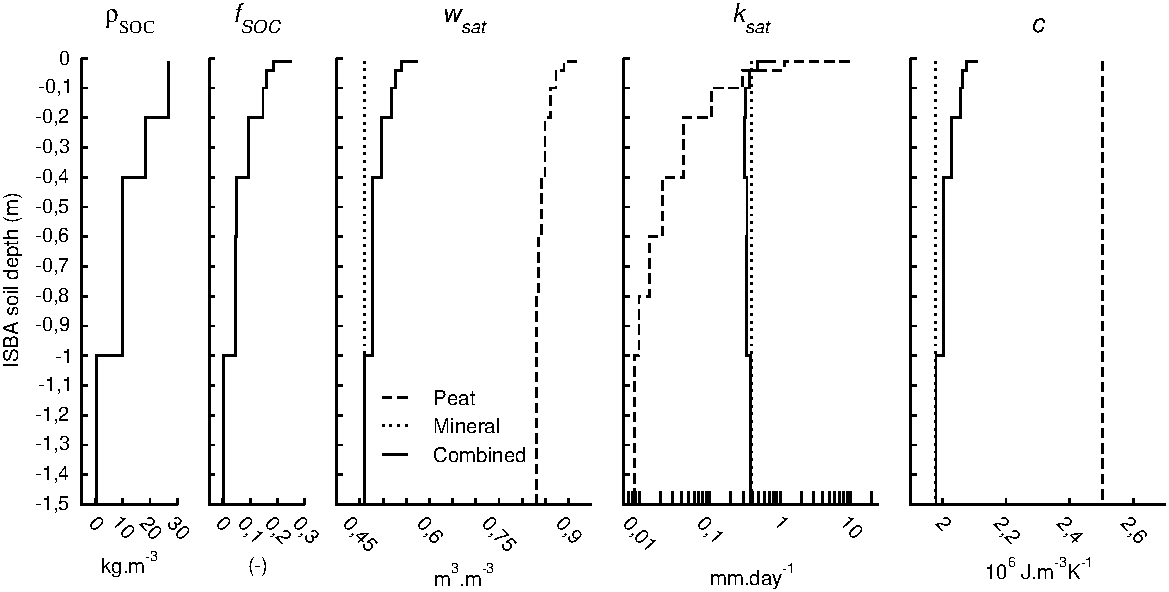
\includegraphics[angle=0, width=12cm, clip=true, trim=4cm 0cm 3cm 0cm]{\EPSDIR/soil_org_carb.pdf}}
\caption{Parameterization of the effect of soil organic carbon (SOC) on soil
hydraulic and thermal properties. The soil organic carbon density
profile, $\rho_{soc}$, is given by 
Eq.~\ref{eq:rho_deep_soil_carbon} 
using a top soil organic
carbon content of 10 kg m$^{-2}$, a sub soil content 
of 15 kg m$^{-2}$, and via
a simple linear interpolation at each soil grid nodes that conserves
the total soil carbon mass. The fraction of the soil that is organic,
$f_{soc}$, in each layer is determined assuming a simple relationship
between this last soil organic carbon density profile and an idealized
peat soil density profile 
(Eq.\ref{eq:frac_soc_soil_carbon}). 
Examples for the soil
porosity, $w_{sat}$, the soil saturated hydraulic conductivity, $k_{sat}$, and
the soil heat capacity, $c$, are given. Dotted lines represent vertical
homogeneous mineral soil properties, dashed lines the idealized peat
soil properties, and plain lines the resulting combined soil
properties using averaging method summed-up in Table~\ref{soil_organic_params}.}
\label{fig:soil_organic_carbon_profiles}
\end{figure}
%%%%%%%%%%%%%%%%%%%%%%%%%%%%%%%%%%%%%%



In ISBA-DF, before averaging soil organic with mineral properties, a
typical peat soil profile is computed for the model soil grid using a
power function for each hydraulic property, $\alpha_{peat}$, found in 
Table~\ref{soil_organic_params}. 
For each soil layer $i$, this function is described as:
%
%%%%%%%%%%%%%%%%%%%%%%%%%%%%%%%%%%%%%
\begin{align}
\label{eq:alpha_peat_soil_carbon}
%
\alpha_{peat}(i) \,\,=&\,\, \alpha_{fibric} \, z(i)^\beta  
\\
\beta \,\,=&\,\,
\frac
{{\rm ln}\left( \alpha_{sapric} / \alpha_{fibric} \right)}
{{\rm ln}\left(d_{sapric} / d_{fibric} \right)}
%
\end{align}
%%%%%%%%%%%%%%%%%%%%%%%%%%%%%%%%%%%%%
%
where $z$ (m) is the depth of the considered soil grid node, $\alpha_{fibric}$ and
$\alpha_{sapric}$ are the fibric and sapric parameter values,
respectively (Table~\ref{soil_organic_params}). 
$d_{fibric}$ (m) is
the depth arbitrarily set to 0.01 m where the profile starts to depart
from fibric values, and $d_{sapric}$ (m) the depth of 1 m where the soil
properties reach the sapric values according to Letts \etal (2000)\nocite{Letts_ea_2000}.

To determine the organic fraction of soil, the density profile of the
soil carbon must be known for the entire soil grid. Using the the
Harmonized World Soil Database (HWSD;
http://webarchive.iiasa.ac.at/Research/LUC/External-World-soil-database/HTML/),
the soil carbon densities in the first 0.3 m, $\rho_{top}$ (kg m$^{-3}$), and the
remaining 0.7 m below, $\rho_{sub}$ (kg m$^{-3}$), are known:
%
%%%%%%%%%%%%%%%%%%%%%%%%%%%%%%%%%%%%%
\begin{subequations}
\label{eq:soil_org_carbon_dens}
\begin{align}
%
\rho_{top} \,\,=&\,\, \frac{S_{top}}{\Delta d_{top}}
\\
\rho_{sub} \,\,=&\,\, \frac{S_{sub}}{\Delta d_{sub}}
%
\end{align}
\end{subequations}
%%%%%%%%%%%%%%%%%%%%%%%%%%%%%%%%%%%%%
%
where $S_{top}$ and $S_{sub}$ (kg m$^{-2}$) are the topsoil and subsoil organic
carbon contents respectively, $\Delta d_{top}$ and $\Delta d_{sub}$
(m) represent the thicknesses of
each observed soil horizon (0.3 and 0.7 m, respectively). We extrapolate
the density below 1 m from this observed near-surface profile
(Eq.~\ref{eq:soil_org_carbon_dens}). 
The extrapolation assumes that the carbon profile
decreases sharply with soil depth according to a power function. The
shape of this function is given by the observed profile if the topsoil
organic carbon density is superior to the subsoil density. Otherwise,
the density of soil carbon below a 1 m depth, $\rho_{deep}$ (kg
m$^{-3}$), 
is taken equal to the subsoil density:
%
%%%%%%%%%%%%%%%%%%%%%%%%%%%%%%%%%%%%%
\begin{equation}
\label{eq:rho_deep_soil_carbon}
%
\rho_{deep} \,\, = \,\,
\left(1-\delta\right) \rho_{sub} 
\,+\,
\delta
\left(
\frac
{S_{top} + S_{sub}}
{\Delta d_{deep} - \Delta d_{top} - \Delta d_{sub} }
\right)
\left[
{\left(
\frac
{\Delta d_{deep}}
{\Delta d_{top} + \Delta d_{sub}}
\right)}^\beta \,-\, 1
\right]
%
\end{equation}
%%%%%%%%%%%%%%%%%%%%%%%%%%%%%%%%%%%%%%%%%
%
where
%
%%%%%%%%%%%%%%%%%%%%%%%%%%%%%%%%%%%%%%%%%
\begin{equation}
\delta \,\, =\,\,\Bigg\lbrace
\begin{matrix}
0 & \forall \, \rho_{top} \leq \rho_{sub}
\\
1 & \forall \, \rho_{top} > \rho_{sub}
%
\end{matrix}
\end{equation}
%%%%%%%%%%%%%%%%%%%%%%%%%%%%%%%%%%%%%
%
and
%
%%%%%%%%%%%%%%%%%%%%%%%%%%%%%%%%%%%%%
\begin{equation}
%
\beta = \frac
{{\rm ln}\left[ 
S_{top}/\left( S_{top} + S_{sub}\right)
\right]}
{{\rm ln}\left[ 
\Delta d_{top}/\left( \Delta d_{top} + \Delta d_{sub}\right)
\right]}
%
\end{equation}
%%%%%%%%%%%%%%%%%%%%%%%%%%%%%%%%%%%%%%%%%
%
Finally, the soil carbon density profile, $\rho_{soc}$ (kg m$^{-3}$), 
over the
entire soil grid is computed using these three soil horizons and a
simple linear interpolation at each grid node that conserves the total
soil carbon mass 
(Fig.~\ref{fig:soil_organic_carbon_profiles}). 
The fraction of the soil that is organic,
$f_{soc}$, in each layer is determined assuming this simple
relationship:
%
%%%%%%%%%%%%%%%%%%%%%%%%%%%%%%%%%%%%%
\begin{equation}
\label{eq:frac_soc_soil_carbon}
%
f_{soc}(i) = \frac
{\rho_{soc}(i)}
{\left[ 1 \,-\, w_{sat,peat}(i) \right]\, \rho_{om}}
%
\end{equation}
%%%%%%%%%%%%%%%%%%%%%%%%%%%%%%%%%%%%%%%%%
%
where $\rho_{om}$ is the pure organic matter density equal 
to 1300 kg m$^{-3}$ (Farouki, 1986)\nocite{farouki1986} and $w_{sat,peat}$ 
the porosity of the peat soil
profile computed using 
Eq.~\ref{eq:alpha_peat_soil_carbon}
and Table~\ref{soil_organic_params}. 
As in Lawrence and Slater (2008)\nocite{Lawrence_Slater_2008}, 
this fraction is used to combine the standard mineral
soil properties with soil organic properties using weighted arithmetic
or geometric averages, depending on the parameter 
(Table~\ref{soil_organic_params}). 
An example of this method is shown in Fig.~\ref{fig:soil_organic_carbon_profiles}
for soil porosity, soil
saturated hydraulic conductivity and soil heat capacity.


%%%%%%%%%%%%%%%%%%%%%%%%%%%%%%
\begin{table}[h]
\caption{
The peat soil hydraulic and thermal parameter values used in ISBA for
fibric and sapric soil. $w_{sat}$ (m$^{3}$ m$^{-3}$) 
is the porosity, $w_{fc}$ (m$^{3}$ m$^{-3}$) 
the water content at field capacity specified as matric potential at
-0.1 bar for peat soil, $w_{wilt}$ (m$^{3}$ m$^{-3}$) 
the water content at wilting
point (matric potential of -15 bar), $b$ the dimensionless shape
parameter of the soil-water retention curve, $\psi_{sat}$ (m) 
the soil matric
potential, $k_{sat}$ (m s$^{-1}$) 
the soil hydraulic conductivity at saturation,
$c$ (J m$^{-3}$ K$^{-1}$) the soil heat capacity of organic matter, 
$\lambda_s$ (W m$^{-1}$ K$^{-1}$)
the thermal conductivity of soil matrix, and $\lambda_{dry}$
(W m$^{-1}$ K$^{-1}$) the dry
soil thermal conductivity. For pedotransfer functions of 
Boelter (1969)\nocite{Boelter_1969}, 
the fiber content in fibric soil is assumed to be equal to
76.8 against 21.8 
in sapric soil in order to reach soil porosity
values close to those of Letts \etal (2000)\nocite{Letts_ea_2000}. The method for averaging
mineral soil properties with peat soil values using the
fraction of soil that is organic is also given for each parameter.
}
\begin{center}
\begin{footnotesize}
\begin{tabular}{llllc}
\hline
$\alpha_{peat}$ & Fibric soil & Sapric soil & Source & Mineral/Peat average \\
\hline
\hline
$w_{sat}$         & 0.9300             &   0.8450          
&    Letts et al. (2000) and Boelter (1969)
&    Arithmetic \\
$w_{fc}$          &  0.3690             &   0.7190          
&     PTF from Boelter (1969) 
&   Arithmetic  \\
$w_{wilt}$       &  0.0730             &   0.2220          
&    TF from Boelter (1969)  
&   Arithmetic  \\
$b$                & 2.7000              &   12.0000         
&     Letts et al. (2000)
&  Arithmetic  \\ 
$\psi_{sat}$     &  -0.0103            &   -0.0101         
&    Letts et al. (2000) 
&  Arithmetic  \\ 
$k_{sat}$        &  2.8$\times 10^{-4}$  & 1.0$\times 10^{-7}$ 
&    Letts et al. (2000)
&  Geometric \\
$c$                & 2.5$\times 10^{-6}$   & 2.5$\times 10^{-6}$ 
&    Farouki (1986)
&    Arithmetic \\
$\lambda_{s}$     &  0.2500             &   0.2500          
&    Farouki (1986) 
&  Geometric   \\
$\lambda_{dry}$  &  0.0500             &   0.0500          
&    Farouki (1986) 
&   Geometric  \\
\hline
\end{tabular}
\end{footnotesize}
\end{center}
\label{soil_organic_params}
\end{table}
%%%%%%%%%%%%%%%%%%%%%%%%%%%%%%%%%%%%

%=========================================================================================================
%=========================================================================================================
\subsection{Treatment of the intercepted water}
%=========================================================================================================
%=========================================================================================================

Rainfall and dew intercepted by the foliage feed a
reservoir of water content $W_r$.  This amount of water
evaporates in the air at a potential rate from the fraction
$\delta$ of the foliage covered with a film of water, as the
remaining part $(1-\delta)$ of the leaves transpires.
%
The fraction of the vegetation covered with water is defined as
%
%%%%%%%%%%%%%%%%%%%%%%%%%
\begin{equation}
\label{eq:meb_delta}
\delta_v = 
\left(1-\omega_{rv}\right)\,\left( \frac{W_{r}}{W_{r,max}} \right)^{2/3}
\,+\, {\frac{\omega_{rv} W_{r}}
{\left(1+a_{rv}\,LAI\right)W_{r,max} - a_{rv}\,W_{r} }}
%
\end{equation}
%%%%%%%%%%%%%%%%%%%%%%%%%
%
Delire et al. (1997)\nocite{Delire1997} 
used
the first term on the RHS of Eq.~\ref{eq:meb_delta} for
relatively low
vegetation 
(Deardorff, 1978)\nocite{Deardorff1978} and
the second term 
for tall vegetation 
(Manzi and Planton, 1994)\nocite{manzi_planton_94}.
%
A weighting function is used which introduces the
vegetation height dependence using the roughness length as a proxy
from
%
%%%%%%%%%%%%%%%%%%%%%%%%%
\begin{equation}
\label{eq:meb_delta_wght}
\omega_{rv} = 2 \,z_{0v} \,-\, 1
\hskip1.in
\left(0 \leq \omega_{rv} \leq 1 \right)
\end{equation}
%%%%%%%%%%%%%%%%%%%%%%%%%
%
where the current value for the dimensionless 
coefficient is $a_{rv}=2$. 

%\begin{equation}
%\delta = {\left( \frac{W_r}{W_{rmax}} \right)}^{2/3}
%\end{equation}

Following Deardorff (1978), we set
\begin{eqnarray}
{\partial W_r \over \partial t} = veg P - (E_v-E_{tr}) - R_r \ ; \
0 \leq W_r \leq W_{rmax}
\end{eqnarray}
where $P$ is the precipitation rate at the top of the vegetation,
$E_v$ is the evaporation from the vegetation including the
transpiration $E_{tr}$ and the direct evaporation $E_r$ when
positive, and the dew flux when negative (in this case $E_{tr} = 0$),
and $R_r$ is the runoff of the interception reservoir.
This runoff occurs when $W_r$ exceeds a maximum value $W_{rmax}$
depending upon the density of the canopy, i.e., roughly proportional
to $veg LAI$.
According to Dickinson (1984), we use the simple equation:
%
%%%%%%%%%%%%%%%%%%%%%%%%%%%%%%%%%%%%%%%%%%%%%%%%%%%%%%
\begin{equation}
\label{eq:isba_max_int_res_cap}
W_{rmax} = c_{wrmax} veg \, LAI 
\end{equation}
%%%%%%%%%%%%%%%%%%%%%%%%%%%%%%%%%%%%%%%%%%%%%%%%%%%%%%
%
Generally speaking, $c_{wrmax}=0.2$ kg m$^{-2}$, although it
can be modified slightly for certain 
vegetation cover.

%=========================================================================================================
%=========================================================================================================
\subsection{Spatial variability of precipitation intensities}
\label{sec:isba_runoff_var_precip}
%=========================================================================================================
%=========================================================================================================

With this option, the main assumption is that, generally, the rainfall intensity is not 
distributed homogeneously over an entire grid cell. As a first-order approximation, the sub-
grid variability in liquid precipitation, $P_i$, can be given by an exponential probability density 
distribution, $f(P_i)$:
     \begin{equation}
      	f(P_i) = \frac{\mu}{P} e^{-\mu\frac{P_i}{P}} 
     \end{equation}

where $P$ represent the mean rainfall rate over the grid cell and $\mu$ a fraction of the grid cell 
affected by rainfall. $\mu$ is calculated using the results of Fan \etal (1996)\nocite{Fan1996}, who showed an 
exponential relationship between the fractional coverage of precipitation and rainfall rate, 
based on their analyses of over 2 years radar observations and rain gauge measurements over 
the Arkansas-Red river basin in the southern plains of the United States. This relationship is:
%
\begin{equation}
  \mu  = 1 - e^{-\beta P}
\end{equation}
%
where $\beta$ is a parameter which depends on grid resolution, $dx$ :
%
\begin{equation}
  \beta = 0.2 + 0.5 e^{-0.001dx}
\end{equation}
%
$dx$ represents represents lengths of square grid cells ranging from 40 km to 500 km. In consequence, the $\mu$ 
parameter is fixed to 1 at high resolution ($\leq 10km$). 
This Spatial variability of precipitation intensities induces a new expression for the 
runoff from the interception reservoir, $W_r$ :
%
\begin{equation}
  W_r = P \times e^{\frac{\mu(W_r-W_{r_{max}})}{P \Delta t}}
\end{equation}
%
The second consequence is that the Horton runoff, $Q_{hort}$, is calculated by integrating the 
difference between the local rainfall and the local maximum infiltration capacity, $I_i$, as 
follows:
%
\begin{equation}
  Q_{hort} = \mu\int^{\infty }_{I_i} \left(P_i - I_i\right) f(P_i) dP_i
  \label{eq:hort}
\end{equation}
%
Another assumption is made on the spatial heterogeneity of the local maximum infiltration 
capacity. Its spatial distribution can also be approximated by an exponential probability 
density distribution:
%
\begin{equation}
  g(I_i) = \frac{1}{\overline{I}}e^{ - \frac{I_i}{\overline{I}}}
\end{equation}

where $\overline{I}$  is the mean maximum infiltration rate over the grid cell. As previously said, $\overline{I}$ is 
calculated for unfrozen and frozen soil conditions. So Eq.\ref{eq:hort} , without snowmelt, can be noted 
as :
%
\begin{eqnarray}
  Q_{hort} &=& \mu 
  (1- \delta_f) \int^{\infty}_{0}\int^{\infty}_{I_{unf,i}}(P_i - I_{unf,i}) f(P_i) g( I_{unf,i})
  dP_i dI_{unf,i} \nonumber \\
  & & +\,
  \mu \delta_f  \int^{\infty}_{0}\int^{\infty}_{I_{f,i}}(P_i - I_{f,i}) f(P_i) g( I_{f,i})
  dP_i dI_{f,i} 
\end{eqnarray}
%
After some mathematical developments, the Horton runoff in presence of rainfall and 
snowmelt, $S_m$, is given following Decharme and Douville (2006)\nocite{Decharme2006a}:
%
\begin{eqnarray}
  Q_{hort} &=& 
  (1- \delta_f) \left( \frac{P}{1+\overline{I_{unf}}\frac{\mu}{P}} + max(0,S_m -\overline{I_{unf}} ) \right) \nonumber \\
  & & + \delta_f \left( \frac{P}{1+\overline{I_{f}}\frac{\mu}{P}} + max(0,S_m -\overline{I_{f}} ) \right) 
  dP_i dI_{f,i}
\end{eqnarray}


%=========================================================================================================
%=========================================================================================================
\subsection{Treatment of the snow}
%=========================================================================================================
%=========================================================================================================

ISBA features several schemes to handle snow on the ground, which are
described below. They range from single-layer schemes with a minimal
number of prognostic variables and highly simplified treatment of snow
thermodynamics, to state-of-the-art multi-layer snowpack schemes
(Explicit Snow -ES- and Crocus). Table \ref{tab:snow-schemes} provides
an summary of the available snowpack schemes and the corresponding
scientific references.

\begin{table}
	\centering
		\begin{tabular}{|l|l|l|}
\hline
Single-layer & D95 & Douville \etal (1995a,1995b) \\
Multi-layer & Explicit-Snow (ES) & Boone (2000); Boone and Etchevers (2001) \\
Multi-layer & Crocus & Brun \etal (1989,1992); Vionnet \etal (2012) \\
\hline 
		\end{tabular}
	\caption{Summary of the snowpack schemes available in ISBA}
	\label{tab:snow-schemes}
\end{table}

%=========================================================================================================
\subsubsection{One-layer snow scheme option}
\label{sec:one_layer_snow_hydro}
%=========================================================================================================

The evolution of the equivalent water content of the snow reservoir
is given by
\begin{eqnarray}
{\partial W_s \over \partial t} = P_s - E_s - M_{lt}
\end{eqnarray}
where $P_s$ is the precipitation of snow, and $E_s$ is the sublimation
from the snow surface.

The presence of snow covering the ground and
vegetation can greatly influence the energy and mass
transfers between the land surface and the atmosphere.
Notably, a snow layer modifies the radiative
balance at the surface by increasing the albedo.
To consider this effect, the albedo of snow $\alpha_s$ is treated
as a new prognostic variable.
Depending if the snow is melting or not,
$\alpha_s$ decreases
exponentially or linearly with time.

If there is no melting (i.e., $M_{lt}=0$):
%
%%%%%%%%%%%%%%%%%%%%%%%%%%%%%%%%%%%
\begin{equation}
\label{eq:albedo_snow_fr_nonmelt}
\alpha_s (t) = \alpha_s (t-\Delta t) - \tau_a {\Delta t \over \tau}
+ { P_s \Delta t \over W_{crn} } ( \alpha_{smax} - \alpha_{smin} ) 
\hskip.5in
\left(\alpha_{smin} \leq \alpha_s \leq \alpha_{smax}\right)
\end{equation}
%%%%%%%%%%%%%%%%%%%%%%%%%%%%%%%%%%%
%
where $\tau_a=0.008$ is the linear rate of decrease per day,
$\alpha_{smin}=0.50$
and $\alpha_{smax}=0.85$ are the minimum and maximum values of the snow
albedo.

If there is melting (i.e., $M_{lt} \ > \ 0$):
%
%%%%%%%%%%%%%%%%%%%%%%%%%%%%%%%%%%%%%%%%
\begin{align}
\label{eq:albedo_snow_fr_melt}
\begin{split}
\alpha_s (t) \,\, =& \,\,  \left[ \alpha_s(t - \Delta t) - \alpha_{smin} \right]
\exp \left[ -\tau_f {\Delta t \over \tau } \right]
+ \alpha_{smin} \\
& + { P_s \Delta t \over W_{crn} } ( \alpha_{smax} - \alpha_{smin} ) 
\hskip2.in
\left(\alpha_{smin} \leq \alpha_s \leq \alpha_{smax}\right)
\end{split}
\end{align}
%%%%%%%%%%%%%%%%%%%%%%%%%%%%%%%%%%%%%%%%%
%
where $\tau_f=0.24$ is the exponential decrease rate per day.
Of course, the snow albedo increases as snowfalls occur, as shown
by the second terms of Eqs.~\ref{eq:albedo_snow_fr_nonmelt}-\ref{eq:albedo_snow_fr_melt}.

The average albedo of a model grid-area is expressed as
\begin{eqnarray}
\alpha_t = (1-p_{sn}) \alpha + p_{sn} \alpha_s
\end{eqnarray}
Similarly, the average emissivity $\epsilon_t$ is also
influenced by the snow coverage:
\begin{eqnarray}
\epsilon_t = (1-p_{sn}) \epsilon + p_{sn} \epsilon_s
\end{eqnarray}
where $\epsilon_s = 1.0$ is the emissivity of the snow.
Thus, the overall albedo and emissivity of the ground for infrared radiation
is enhanced by snow.

Because of the significant variability of thermal properties related
with the snow compactness,
the snow density, $\rho_s$, is also considered
as a prognostic variable.
Based on Verseghy (1991)\nocite{Verseghy1991}, $\rho_s$ decreases exponentially at a rate
of $\tau_f$ per day:
%
%%%%%%%%%%%%%%%%%%%%%%%%%%%%%%%%%%%%%%%%%%%%
\begin{equation}
\rho_s(t)=\left[ \rho_s(t-\Delta t) - \rho_{smax} \right]
\exp \left[ -\tau_f {\Delta t \over \tau } \right] + \rho_{smax}
+ {P_s \Delta t \over W_s} \rho_{smin}  
\hskip.4in
\left(\rho_{smin} \leq \rho_s \leq  \rho_{smax}\right)
\end{equation}
%%%%%%%%%%%%%%%%%%%%%%%%%%%%%%%%%%%%%%%%%%%%
%
where
$\rho_{smin}=$ 100 and $\rho_{smax}=$ 300 kg m$^{-3}$
are the minimum and maximum snow densities.

%Finally, the average roughness length $z_{0t}$ is
%\begin{eqnarray}
%z_{0t} = ( 1 - p_{snz0} ) z_0 + p_{snz0} z_{0s}
%\end{eqnarray}
%where
%\begin{eqnarray}
%p_{snz0} = { W_s \over W_s + W_{crn} + \beta_s g z_0 }
%\end{eqnarray}
%Here, $\beta_s = 0.408 \ s^2 m^{-1}$ and $g=9.80665 \ m s^{-2}$ are physical constants,
%whereas $z_{0s}$ is the roughness length of the snow.

%=========================================================================================================
\subsubsection{Multi-layer snow scheme options}
\label{sec:isba_multi_layer_snow}
%=========================================================================================================

Two multi-layer snow schemes options are available in ISBA, namely Explicit Snow (ES)
and Crocus. Explicit Snow (Boone and Etchevers,
2001\nocite{Boone2001}; Decharme et al. 2016) is a so-called intermediate complexity scheme which
is representative of a class of snow models which
use several layers and have simplified physical parameterization
schemes (Loth \etal 1993\nocite{Loth1993}; Lynch-Stieglitz, 1994\nocite{Lynch-Stieglitz1994}; Sun \etal 1999\nocite{Sun1999}).
In contrast, Crocus features a detailed description of processes
occurring within the snowpack (Brun \etal 1989; 1992\nocite{brun1989,brun1992}; Vionnet \etal 2012\nocite{Vionnet2012}).
Crocus was initially a stand-alone model, and it was recently coupled to ISBA building on the ES model structure. 
In what follows, the description 
applies to both ES and Crocus unless otherwise stated.


Compared to the baseline ISBA snow scheme,
the explicit multi-layered approach shared by ES and Crocus 
resolves the large thermal and the density gradients
which can exist in the snow cover, distinguishes the surface
energy budgets of the snow and non-snow covered portions
of the surface, includes the effects of liquid water storage
in the snow cover, computes the
absorption of incident radiation within the pack,
and calculates explicit heat conduction between the
snow and the soil. Figure \ref{fig:schema-crocus} provides an overview
of the processes handled in the multi-layer snow schemes, coupled to
the soil and vegetation components of ISBA. 

The multi-layer snowpack schemes Crocus and ES are most consistently
used together with ISBA-DF rather than the force-restore soil
schemes. In addtion, Crocus handles snow metamorphism, i.e. the
physical transformations of snow grains through time, and
interactively modifies the vertical discretization of the vertical
grid of snow layers to optimize the representation of internal snow
processes. In practice, Crocus is generally run with a larger total
possible number of snow layers than ES. ES typically uses up to 12
snow layers, while standard Crocus runs use up to 20 or 50 snow
layers. The latter configuration is appropriate when the focus is
placed on the study of the properties of the snowpack itself
(avalanche hazard prediction, snow physical properties, combined use
of remote sensing).

\begin{figure}[h!]
\begin{center}
\psfig{figure=\EPSDIR/process_variables_soil.pdf,width=11cm}
%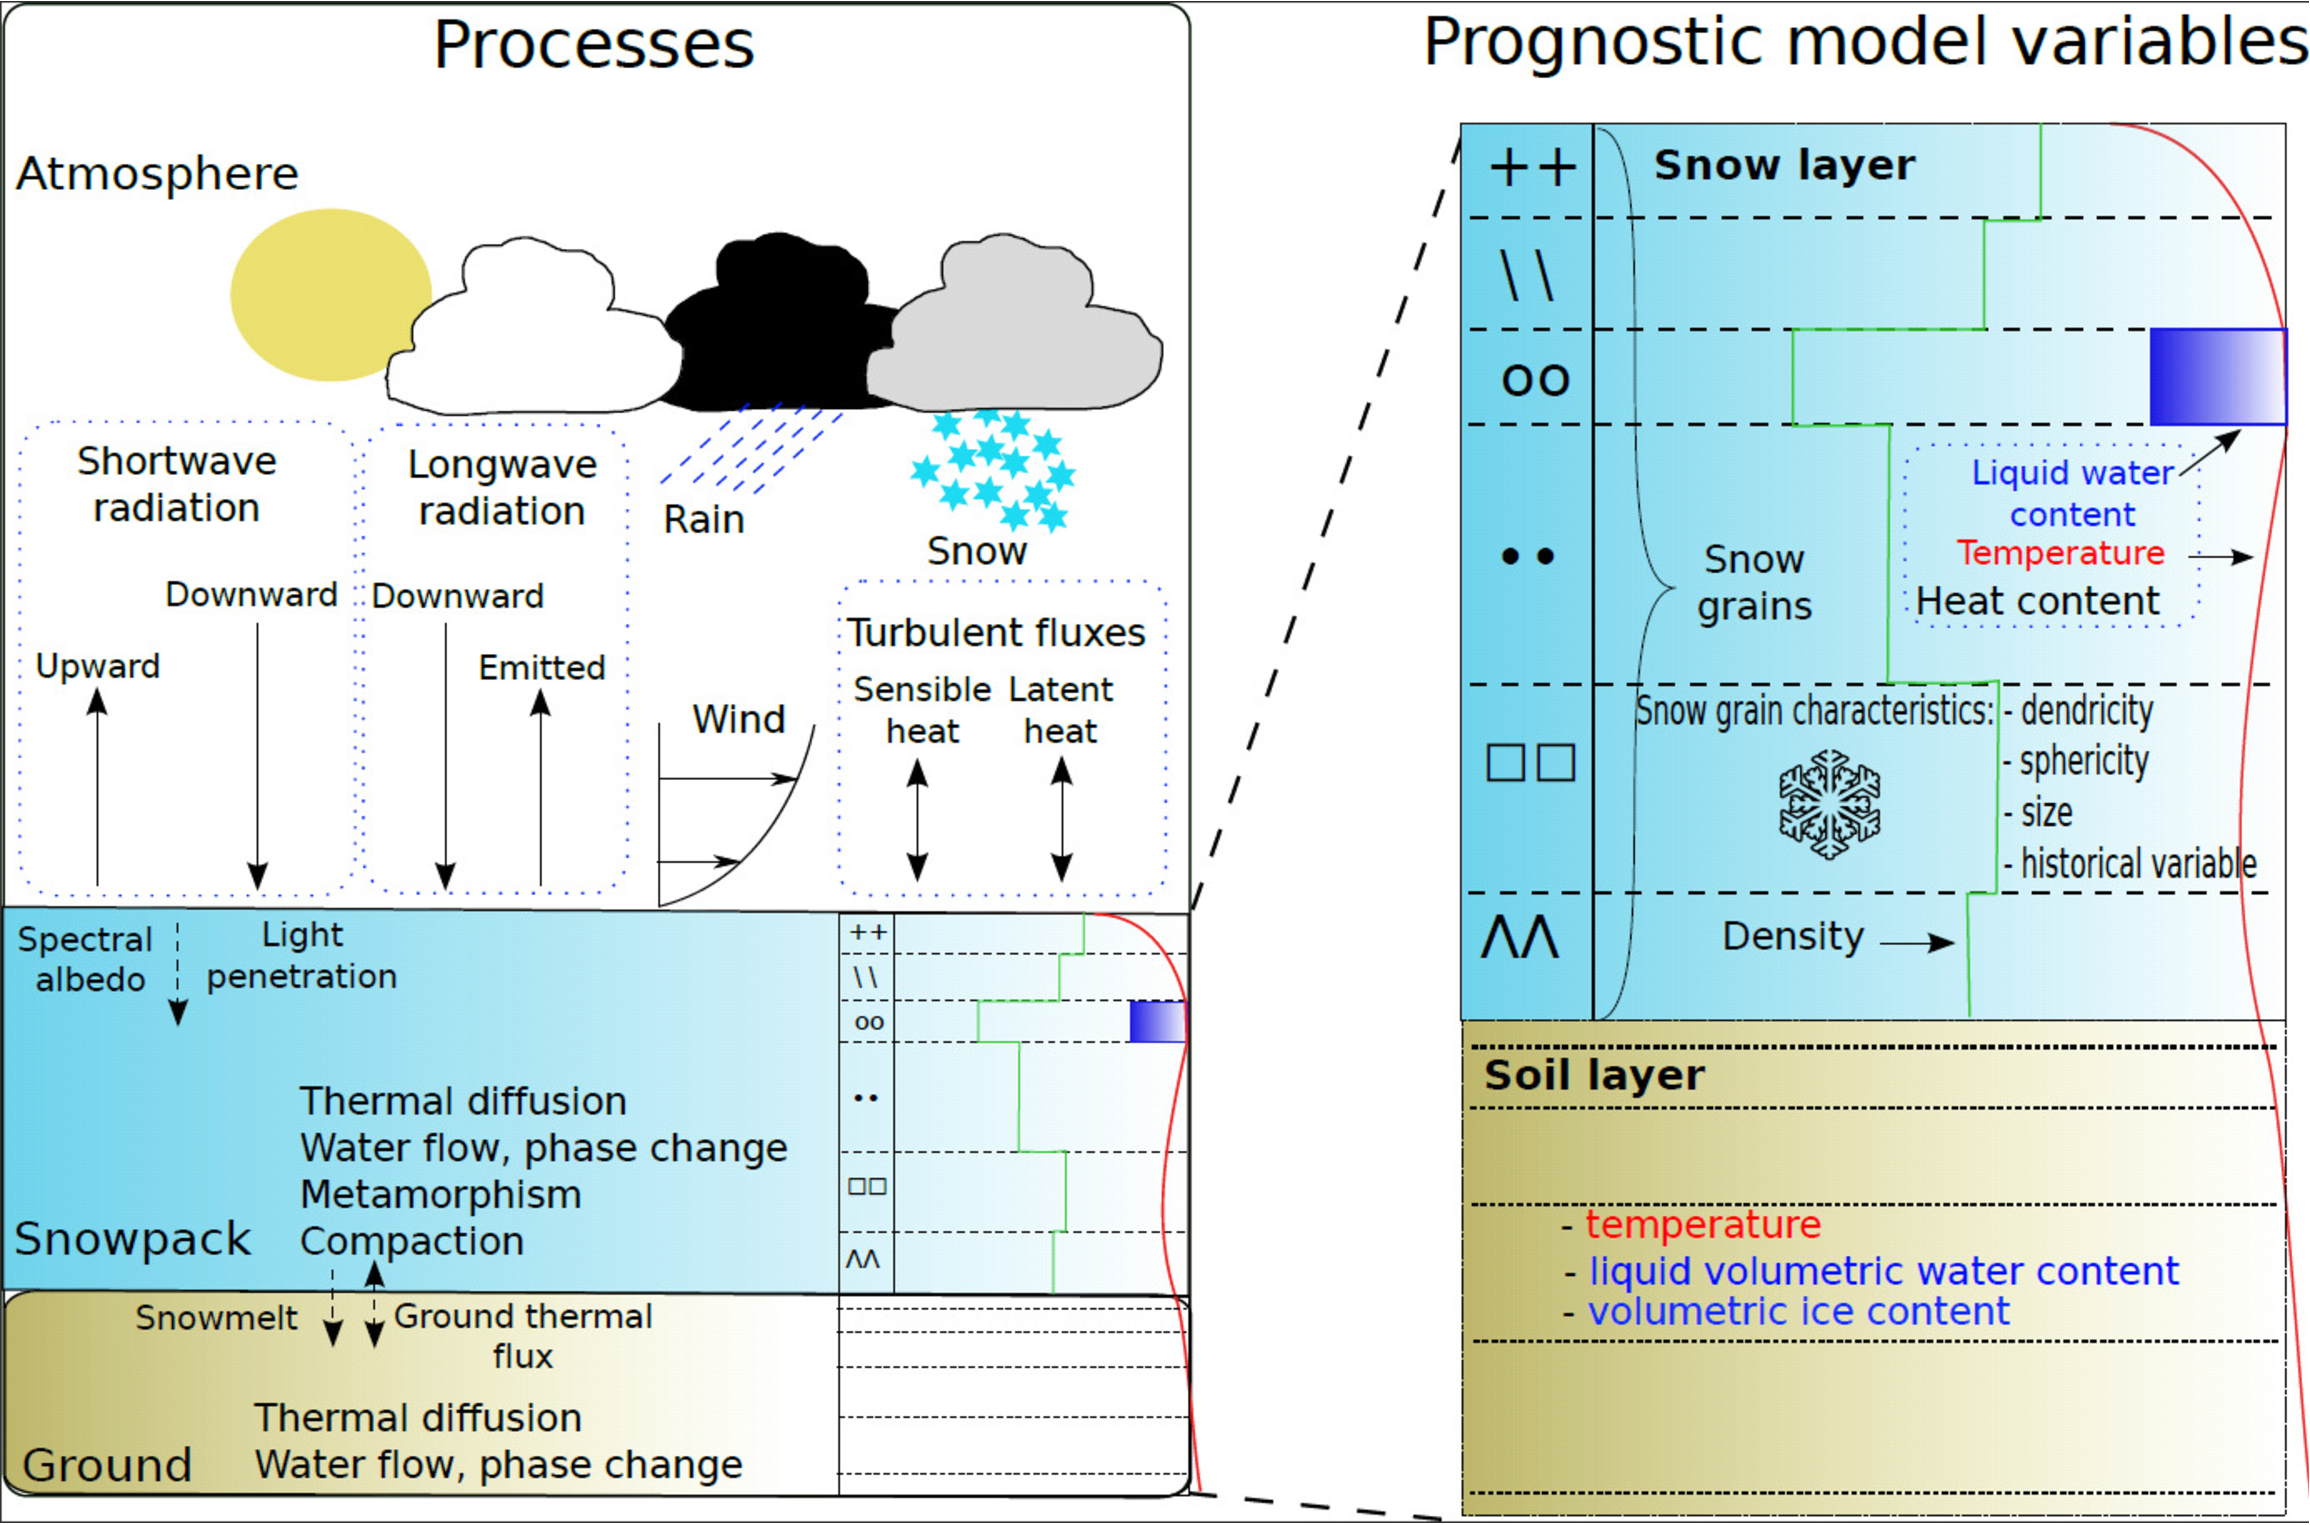
\includegraphics[width = 0.9\linewidth]{\EPSDIR/process_variables_soil.pdf}
\caption{Overview of the physical processes and prognostic variables
  used to characterize the snowpack in the multi-layer snowpack
  schemes options of ISBA (ES and Crocus). The  major differences
  between the ES and Crocus scheme is that ES does not treat snow
  metamorphism explicitly, and that the number of snow layers is kept
  significantly lower than for Crocus (on the order of 3 typically,
  vs. up to 20 or 50 for Crocus. \label{fig:schema-crocus}}
\end{center}
\end{figure}

The conservation equation for the total snow cover mass
is expressed as
%
\begin{eqnarray}
{\partial W_s \over \partial t} =
P_s + p_{sn}\,\left(P-P_s\right) - E_{s} - E_{sl} - Q_n
\,\,\,,
\end{eqnarray}
%
where $E_{sl}$ represents evaporation of liquid water
from the snow surface, and the product $p_{sn}\,\left(P-P_s\right)$
represents the portion of the total rainfall that is
intercepted by the snow surface while the remaining
rainfall is assumed to be intercepted by the snow-free soil and vegetation
canopy. The snow-runoff rate, $Q_n$,
is the rate at which
liquid water leaves the base of the snow cover.


The snow state variables are the heat content ($H_s$),
the layer thickness ($D$), and the layer average density ($\rho_s$).
The temperature ($T_{sn}$) and liquid water content ($w_{sl}$) are defined
using the heat content.
The use of the Crocus scheme induces the definition of further variables, 
which describe the morphological properties of snow grains ($d$ dendricity, $s$ sphericity, 
$g_s$ grain size, $h$ historical variable and $A$ age of a given snow layer). 
See Vionnet \etal (2012) for details.

The total snow depth, $D_s$ (m) is defined as
%
\begin{eqnarray}
D_s = \sum_{i=1}^{N_s} D_i
\end{eqnarray}
%
where a 12-layer configuration is currently used by default (i.e. $N_s=12$). 
In ES and Crocus, the thickness of the surface snow layer can be
as low as 1 mm although it typically ranges on the order of 0.01 to 0.02 m.
The thickness of internal snow layers is on the order of a
few cm typically, with a finer mesh towards the air/snow and
ground/snow interface. See Vionnet \etal (2012) and Decharme \etal
(2016) for details.

The evolution of snow density in each layer is due to snow compaction
resulting from changes in snow viscosity (Brun \etal 1989) and
wind-induced densification of near surface snow layers  
(Brun \etal 1997). This wind-driven compaction process is assumed to occur
when wind velocity exceeds a threshold value that depends on snow
surface characteristics. This process is especially important for
simulating the evolution of the snow density over polar regions. 
%
In ES, additional changes arise from snowfall which generally reduce the
snow density and more details can be seen in Decharme \etal (2016). In
Crocus, snowfall induces the creation of a new snow layer at the
surface ; mechanical settling is computed using a Newtonian formalism
where the viscosity depends mostly on the snow density and temperature
but also on the snow type (see Vionnet \etal 2012, for
details). When Crocus is used, the slope angle has an impact on the
compaction rate, since only the component of the weight perpendicular
to the snow layering need be taken into account. In practice, the
acceleration of gravity ($g=9.80665$ m s$^{-2}$) is then simply multiplied
by cos($slope_i$) where $slope_i$ is the slope of the grid point $i$.

The snow heat content (J m$^{-2}$) is defined as
%
\begin{eqnarray}
H_{s\,i} = c_{s\,i}\,D_i\,\left(T_{sn\,i}-T_0\right)
\,-\, L_f\,\rho_w \left(w_{s\,i}- w_{sl\,i}\right)\,\,\,,
\end{eqnarray}
%
where $w_s$ is the total snow layer water equivalent depth (m),
$w_{sl}$ is the snow layer liquid water content (m), and $c_s$
is the snow heat capacity (J m$^{-3}$ K$^{-1}$) (using the same
definition as the baseline ISBA snow scheme).
The snow heat content is used in order to allow
the presence of either
cold (dry) snow which has a temperature less
than or equal to the freezing point
%and contains no liquid water,
or warm (wet)
snow which is characterized by a temperature at the freezing point
and contains water in liquid form.
The snow temperature
and liquid water content can then be defined as
%
\begin{eqnarray}
T_{sn\,i} &=& T_f \,+\, \left(H_{s\,i}  + L_f\,\rho_w\,w_{s\,i}\right)
/\left(c_{s\,i}\,D_i \right) \,;
\hskip.3in
w_{l\,i} = 0 \\
%
w_{sl\,i} &=& w_{s\,i} \,+\, \left(H_{s\,i}/L_f\,\rho_w\right) \,;
\hskip1.3in
T_{sn\,i} = T_f \,\,\,{\rm and} \,\,\, w_{sl\,i} \leq w_{sl\,{\rm max}\,i}
\end{eqnarray}
%
where $w_{sl\,{\rm max}\,i}$ is the maximum liquid water
holding capacity of a snow layer,
which is based on empirical relations. All
water exceeding this flows into the layer below where
it can do one or all of the following:
add to the liquid water content, refreeze, or continue
flowing downward. 

Snow heat flow is along the thermal gradient
as any snow melt or percolated water within the snow cover
is assumed to have zero heat content.
The layer-averaged snow temperature equation
($T_{s\,i}$) is expressed as
%
\begin{eqnarray}
c_{s\,i} D_i {\partial T_{sn\,i}\over\partial t}
= G_{s\,i-1} - G_{s\,i} + R_{s\,i-1} - R_{s\,i}  - S_{s\,i}
\,\,\,,
\end{eqnarray}
%
where $S_s$ represents an energy sink/source term associated with
phase changes between the liquid and solid phases of water.
Incoming short wave radiation ($R_s$)
transmission within the snowpack decreases exponentially
with increasing snow depth. At the surface, it is expressed as
%
\begin{eqnarray}
R_{s\,0} = R_g \,\left(1-\alpha_s\right)
\end{eqnarray}
%
where the snow albedo is defined  following Brun \etal (1992). In ES
and Crocus the solar radiation is handled using three separate
spectral bands ([0.3-0.8], [0.8-1.5] and [1.5-2.8] $\mu$m). First of all,
the albedo is computed in each band, as a function of the snow
properties in the first snowpack layer for ES and the top 0.03 m of the
snowpack for Crocus. In the UV and visible range ([0.3-0.8] $\mu$m), snow
albedo depends mostly on the amount of light absorbing impurities, but
also on its micro-structure. The latter is represented by the optical
diameter of snow, $d_{opt}$, which corresponds to the diameter of a
collection of mono-dispersed ice spheres possessing the same
hemispherical albedo as the corresponding semi-infinite snow
layer. The impact of snow browning due to the deposition of light
absorbing impurities is parametrized from the age of the uppermost
snow layer. In the near-infrared bands, the spectral albedo depends
only on the optical diameter of snow. The optical diameter of
snow is currently empirically derived from the snow density and age
for ES (Decharme \etal 2016) and the microstructure properties of the
snow for Crocus (see below, and Vionnet \etal 2012). Once the
spectral albedo is calculated, in every spectral band the incoming
radiation is depleted according to the albedo value, and the remaining
part penetrates the snowpack and is gradually absorbed in the snow
layers assuming an exponential decay of radiation with depth. The
solar flux, $Q_s$, at a depth $z$ below the snow surface is expressed as
follows:
%
%%%%%%%%%%%%%%%%%%%%%%%%%%%%%%%%%%%%%%%%%%%%%%%%%%%%%%%%%%%%%%%
\begin{equation}
Q_s = SW\downarrow \, \sum^3_{k=1}
\Bigg\lbrace
\omega_k \left(1-\alpha_k\right)
{\rm exp}\left[
-\sum^i_{j=1}
\left(
\beta_{k,j}\,\Delta z_j \, 
\right)
\right]
\Bigg\rbrace
\end{equation}
%%%%%%%%%%%%%%%%%%%%%%%%%%%%%%%%%%%%%%%%%%%%%%%%%%%%%%%%%%%%%%%
%
where $SW\downarrow$ represents the incoming solar radiation, 
$\alpha_k$ the albedo and $\beta_{k,j}$ 
the absorption coefficient for the spectral band
$k$ and layer $j$. In the current version, the incoming shortwave
radiation Rs is split into three bands using empirical coefficients $\omega_k$
equal to 0.71, 0.21 and 0.08 respectively for bands [0.3-0.8], [0.8-1.5]
and [1.5-2.8] mm. Future developments will allow for forcing
where incoming shortwave radiation is partitioned into several
bands. Finally, shortwave radiation excess for thin snow cover (transmitted
through the snow) is added to the snow/ground heat flux.

The sub-surface heat ($G_s$) flux terms are evaluated using
simple diffusion. At the surface, this flux is expressed as
%
\begin{eqnarray}
G_{s\,0}
= \epsilon_s \left( R_A - \sigma_{SB} {T_{sn\,1}}^4 \right)
\,-\, H\left(T_{sn\,1}\right) \,-\, LE\left(T_{sn\,1}\right) \,-\,
c_w \,p_{sn} \left(P-P_s\right)\left(T_f-T_r\right)\,\,\,,
\end{eqnarray}
%
The last term on the right hand side of the above equation
represents a latent heat source when rain
with a temperature ($T_r$) greater than $T_0$ falls on the snow cover,
where $c_w$ represents the heat
capacity of water (4187 J kg$^{-1}$ K$^{-1}$).
Rainfall is simply assumed to have a temperature which is the larger of
the air temperature ($T_a$) and the freezing point.
The latent heat flux from the snow
includes the liquid fraction weighted
contributions from the
evaporation of liquid water and sublimation.

The ISBA surface soil/vegetation layer temperature is then
coupled to the snow scheme using
%
%%%%%%%%%%%%%%%%%%%%%%%%%%%%%%%%%%%%%%%%%%%%%%
\begin{align}
\begin{split}
{1\over C_T}{\partial T_s\over\partial t} \,\, = &\,\, 
\left(1-p_n\right) 
\left[
R_g\left(1-\alpha\right) +
\epsilon_t\left(R_A-\sigma {T_s}^4\right)- H - LE
- {2\pi \over C_T \tau} \left(T_s-T_2\right)
\right] 
\\
%
& 
\hskip.2in
\,+\, p_n \,\, \left( G_{s\,N}+R_{s\,N}
%+ c_w\,Q_n\,\left(T_f-T_s\right)
\right)
\end{split}
\end{align}
%%%%%%%%%%%%%%%%%%%%%%%%%%%%%%%%%%%%%%%%%%%%%%
%
%The term on the right hand side of the above equation
%involving the snow runoff ($Q_n$) represents an advective term.
The net surface fluxes to/from the atmosphere
are then calculated as the snow-cover
fraction weighted sums over the snow and non-snow covered
surfaces. When either multi-layer option is used (ES or Crocus), the single-layer snowpack scheme in ISBA 
is used when the snow cover is relatively thin (arbitrarily
defined as 0.05 m depth). When the snow depth exceeds this
threshold, the snow mass and heat is transferred to the chosen multi-layer
scheme. This prevents numerical difficulties
%and a more complex computer code
for vanishingly thin snow packs.

%=========================================================================================================
\subsubsection{Additional features of the Crocus scheme}
%=========================================================================================================

{\it Evolution of the vertical discretization of the finite-element grid}

The dynamical evolution of the number and thicknesses of the numerical
snow layers is a key and original feature of Crocus, which aims at
simulating  the vertical layering of natural snowpacks in the best
possible way. The maximum number of numerical layers is an important
user-defined set-up option. A minimum of 3 layers is imposed for
solving the heat conduction through the snowpack but there is no
limitation on the maximum number. As the maximum number of layers
increases, the snowpack stratigraphy can be simulated in more
detail. According to the research or operational objectives, the user
has to find the appropriate balance between the realism and the
computational cost of the simulation. An important point to mention is
that the snowpack scheme dynamically manages a different vertical grid
mesh, in terms of the number and the thickness of snow layers, for
each grid point when it is run in parallel mode for a spatially
distributed simulation ; this is a common case for snow/atmosphere
coupled simulations or for distributed stand-alone simulations. 


The adjustment of the snowpack layering is achieved with a set of
rules. The procedure is activated at the beginning of each time step
according to the following sequence:

\begin{itemize}

 \item for snowfall over a bare soil, the snowpack is built up from
   identical layers, in terms of thickness and state variables. Their
   number depends on the amount of fresh snow and on the maximum
   number of layers;

\item  for snowfall over an existing snowpack, it is first attempted
  to incorporate the freshly fallen snow into the existing top layer,
  provided its grain characteristics are similar and its thickness is
  smaller than a fixed limit. The similarity between two adjacent
  layers is determined from the value of the sum of their differences
  in terms of $d$, $s$ and $g_s$, each weighted with an appropriate
  coefficient. If the merging is not possible, a new numerical layer
  is added to the preexisting layers. If the number of layers then
  reaches its maximum, a search is carried out to identify two
  adjacent layers to be merged. This is done by minimizing a criterion
  balancing the similarity between their respective grain
  characteristics and their thicknesses;

\item for no snowfall, a check is carried out to see whether it is
  convenient to merge too thin snow layers or to split thoses which
  are thick. This is achieved by comparing the present thickness
  profile to an idealized profile, which acts as an attractor for the
  vertical grid. This idealized thickness profile depends on the
  current snow depth and on the user-defined maximal number of layers
  (see Figure \ref{fig:crocus-grid} for an example). Merging two
  layers is only possible for those which are similar enough in terms
  of grain characteristics. Grid resizing affects only one layer per
  time step, with a priority given to the surface and bottom layers,
  in order to accurately solve the energy exchanges at the surface and
  at the snow/soil interface;

\item for most time steps, no grid resizing is carried out, except
  that the thickness of each layer decreases according to its
  compaction rate.

\end{itemize}

The consistency of the physical prognostic variables is maintained in
case of grid resizing. A projection is achieved from the former
vertical grid to the new one. Mass, heat content and liquid water
content are conserved.  When a new numerical snow layer is built from
several former layers, its grain characteristics are calculated in
order to conserve the averaged weighted optical grain size of the
former layers. This insures a strong consistency in the evolution of
surface albedo, even when frequent grid resizing occur at the surface
in case of frequent snowfalls or surface melting events.


\begin{figure}[h!]
\begin{center}
%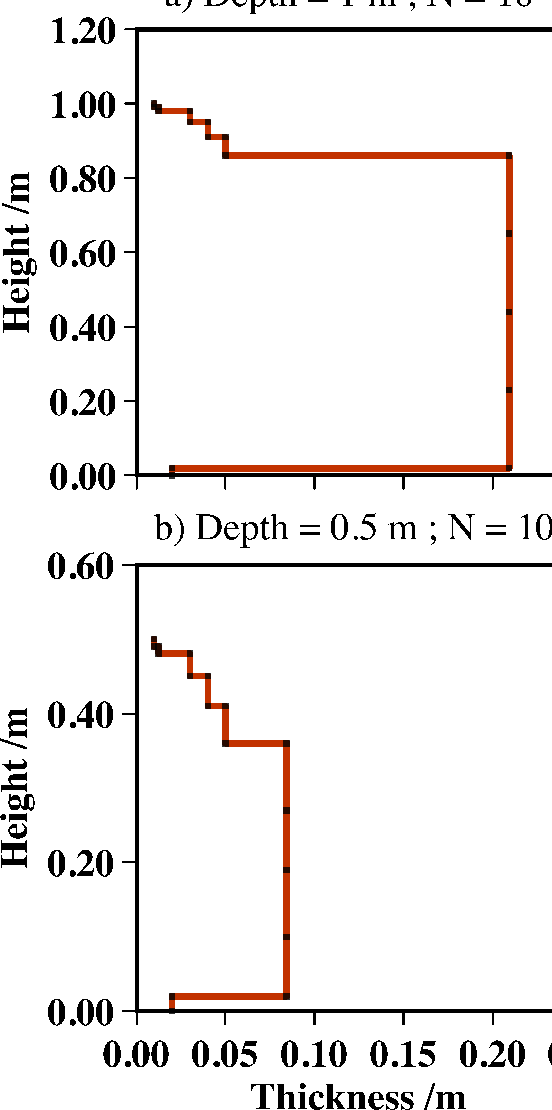
\includegraphics[width = 0.5\linewidth]{crocus-grid.pdf}
\psfig{figure=\EPSDIR/crocus-grid.pdf,width=7cm}
\caption{Illustration of the optimal vertical grid of Crocus, which
  depends on total snow depth and on the user-defined maximum number
  of snow layers. \label{fig:crocus-grid}}
\end{center}
\end{figure}


{\it Snow metamorphism}

Snow metamorphism is implemented in the snowpack scheme Crocus through
a set of quantitative laws describing the evolution rate of the type
and size of the snow grains in each layer (Brun \etal 1992). This is
carried out within the subroutine. A distinction is made between
dendritic and non-dendritic snow. Snow falls as dendritic snow and
remains dendritic until $d$ reaches 0. Snow then reaches the state of
rounded crystals, faceted crystals or belongs to an intermediate
state. It is is then characterized by its sphericity ($s$), ranging
from 0 to 1, and a grain size, $g_s$, ranging from 0.3 to 0.4 mm. Such
snow is defined as non-dendritic. The metamorphism laws that govern
the evolution of snow grain depend on temperature, the temperature
gradient, and include wet metamorphism. They are similar to the laws
initially described by Brun \etal (1992) and are mostly based on
empirical fits to experimental data. The metamorphism laws that govern
the evolution of snow grain are given in Table~\ref{tab_metamo_dry}
and~\ref{tab_metamo_wet}, respectively for dry and wet
metamorphism. In the case of temperature gradient metamorphism, fits
to experimental data by Marbouty (1980)\nocite{marbouty1980} are
used. In this case, the increase of grain size $g_s$ follows:
%
\begin{equation}
\frac{\delta g_s}{\delta t} = f(T)h(\rho)g(G)\Phi
\end{equation}
where G is the absolute value of the temperature gradient $(|\delta T
/ \delta z|)$ and $f$, $g$, $h$ and $\Phi$ are dimensionless functions
varying from 0 to 1 given by:
%
\begin{equation}
f = \left\{
    \begin{array}{ll}
       0 & \mbox{if}\quad T-T_{\rm fus}  < -40~\mathrm{K} \\
       0.011\times(T-T_{\rm fus}+40) & \mbox{if} \quad -40\le T-T_{\rm fus}< -22~\mathrm{K}  \\
       0.2+0.05\times(T-T_{\rm fus}+22) & \mbox{if} \quad -22\le T-T_{\rm fus}< -6~\mathrm{K}  \\     
       1-0.05\times(T-T_{\rm fus})&\mbox{otherwise}
    \end{array}
\right.
\label{eqn_fmarb}
\end{equation}
where $T_{\rm fus}$  is temperature of the melting point for water (K), and $h$, $g$ and $\Phi$ are given below:
\begin{equation}
\Phi = 1.0417.10^{-9}~\mathrm{m\,s}^{-1}
\label{eqn_phimarb}
\end{equation}
\begin{equation}
h = \left\{
    \begin{array}{ll}
       1.& \mbox{if}\quad\rho < 150 \quad \mbox{kg\,m}^{-3}\\
       1-0.004\times(\rho-150) & \mbox{if}\quad 150<\quad\rho < 400 \quad \mbox{kg\,m}^{-3}\\     
       0.& \mbox{otherwise}
    \end{array}
\right.
\label{eqn_hmarb}
\end{equation}
\begin{equation}
g = \left\{
    \begin{array}{ll}
       0. & \mbox{if}\quad G < 15~\mathrm{K\,m}^{-1} \\
       0.01\times(G-15) & \mbox{if} \quad 15\le G< 25~\mathrm{K\,m}^{-1}  \\
       0.1+0.037\times(G-25) & \mbox{if} \quad 25\le G< 40~\mathrm{K\,m}^{-1} \\   
       0.65+0.02\times(G-40) & \mbox{if} \quad 40\le G< 50~\mathrm{K\,m}^{-1} \\
       0.85+0.0075\times(G-50) & \mbox{if} \quad 50\le G< 70~\mathrm{K\,m}^{-1} \\    
       1. &\mbox{otherwise}
    \end{array}
\right.
\label{eqn_gmarb}
\end{equation}


\begin{table}[t]
\caption{Metamorphism laws under dry conditions. G is the vertical temperature gradient $(|\delta T / \delta z|) $, $T$ the temperature (K) and $t$ is time expressed in days. $f$, $g$, $h$ and $\Phi$ are empirical functions to predict depth-hoar growth-rate from Marbouty (1980).}
\vskip4mm
\centering
\begin{tabular}{c|c|c}
\hline
&Non-dendritic snow &Dendritic snow \\
\hline
\multirow{2}{*}{ $G$ $\leq$ 5 K.m$^{-1}$} & $\frac{\delta s}{\delta t} = 10^9e^{-6000/T}$ & $\frac{\delta d}{\delta t} = -2.10^8e^{-6000/T}$ \\
& $\frac{\delta g_s}{\delta t} = 0$ &$\frac{\delta s}{\delta t} = 10^9e^{-6000/T}$ \\
%\middlehline
\hline
\multirow{2}{*}{5 $<$ $G$ $\leq$ 15 K.m$^{-1}$} & $\frac{\delta s}{\delta t} = -2.10^8e^{-6000/T}G^{0.4}$ &\multirow{2}{*}{$\frac{\delta d}{\delta t} = -2.10^8e^{-6000/T} G^{0.4}$} \\
& $\frac{\delta g_s}{\delta t} = 0$ &\\
\cline{1-2}
\multirow{2}{*}{$G$ $>$ 15 K.m$^{-1}$} & if $s>$0: $\frac{\delta s}{\delta t} = -2.10^8e^{-6000/T}G^{0.4}$ and $\frac{\delta g_s}{\delta t} = 0$ & \multirow{2}{*}{$\frac{\delta s}{\delta t} = -2.10^8e^{-6000/T} G^{0.4}$} \\
& if $s=$0: $\frac{\delta s}{\delta t} = 0$ and $\frac{\delta g_s}{\delta t} = f(T)h(\rho)g(G)\Phi$ & \\
\hline
\end{tabular}
\label{tab_metamo_dry}
\end{table}

\begin{table}[t]
\caption{Metamorphism laws in the presence of liquid water. $\theta$ is the mass liquid water content and $t$ is time expressed in days. $v$ refers to the equivalent volume of snow grain and $v'_0$ and $v'_1$ are empirical constants taken from Brun (1989).}
\vskip4mm
\centering
\begin{tabular}{c|c|cc}
\cline{1-3}
\cline{1-3}
&Non-dendritic snow &Dendritic snow & \\
\cline{1-3}
\multirow{2}{*}{0 $\leq$ $s$ $<$ 1} & $\frac{\delta g_s}{\delta t} = 0$ & \multirow{2}{*}{ $\frac{\delta d}{\delta t} = -\frac{1}{16} \theta^3$ }&  \\
& $\frac{\delta s}{\delta t} = \frac{1}{16} \theta^3$ & &with $ \theta = 100\frac{W_{\rm liq}}{\rho D}$\\
\cline{1-2}
\multirow{2}{*}{$s$ $=$ 1} & $\frac{\delta s}{\delta t} = 0$ &\multirow{2}{*}{$\frac{\delta s}{\delta t} = \frac{1}{16} \theta^3$} &\\
& $\frac{\delta v}{\delta t} = v'_0+v'_1 \theta^3$ && \\
\cline{1-3}
\end{tabular}
\label{tab_metamo_wet}
\end{table}

In addition to this default metamorphism formulations, three other formulations 
of metamorphism can be activated. The first one (C13) is similar to the default 
one but uses the optical diameter and the sphericity as prognostic variables. 
The second one (T07) is based on the parameterizations from Taillandier \etal (2007)
\nocite{taillandier2007}%\citet{Taillandier2007} 
and Domine \etal (2007) \nocite{domine2007}%\citet{Domine2007}
and the last one (F06) is based on the parameterizations 
from Flanner \etal (2006) \nocite{flanner2006}.%\citet{Flanner2006}
For detail of these implementations please refer to Carmagnola \etal (2014) 
\nocite{Carmagnola2014}.%\citet{Carmagnola 2014}

{\it Snow radiative transfer scheme}

In addition to the basic formation of solar energy absorption and snow albedo 
over three spectral bands described above, a new option is available for solar 
radiative transfer calculation in the snowpack. The radiative scheme is called 
TARTES Libois \etal (2013) \nocite{libois2013}%\citep{Libois2013} 
(Two-streAm Radiative TransfEr in Snow model). TARTES 
is a two-stream radiative transfer scheme based on an analytical formulation of 
radiative transfer in snow (Kokhanovsky \etal (2004))\nocite{kokhanovsky2004}.
%\citep{Kokhanovsky2004}
TARTES computes spectral  solar absorption within each layer and diagnoses spectral 
and broadband albedo. The default spectral resolution is 20 nm. The scheme uses 
spectral solar irradiance calculated from input broabdand data using a parameterization 
derived from SBDART (Ricchiazzi \etal (1998))\nocite{ricchiazzi1998} %\citep{Richiazzi1998} 
at Col de Porte site. The scientific documentation of TARTES is available at 
http://lgge.osug.fr/~picard/tartes/. 

TARTES simulates the effect of light absorbing impurities as an equivalent 
black-carbon content. To this respect, three options can be activated :

\begin{itemize}
\item "TA1": no impurity
\item "TA2":  snow impurity content constant to 100 ng g$^{-1}$
\item "TAR" : impurity content = 2*snow age ng g$^{-1}$
\end{itemize} 

{\it Effects of wind}

{\bf{
			\begin{center}
			\begin{tabular}{|l|}
\hline
 \textcircled{!} As a 1D model, the continental surface scheme ISBA within SURFEX is \\
 NOT designed to handle explicitly wind-induced snow redistribution. \\
 Indeed, grid points are treated independently from each other. \\
 Nevertheless, the Crocus snowpack scheme includes parameterizations \\
 that represent some effects of wind drift on the snowpack.  \\
\hline
			\end{tabular}
			\end{center}

}}

The compaction and the metamorphism of the surface layers during wind
drift events are taken into account in a simplified way, as described
initially by Brun \etal (1997). A mobility index, $M_{\rm O} $,
describes the potential for snow erosion for a given snow layer and
depends on the microstructural properties of snow ($d$, $s$ and
$g_s$):
%
\begin{equation}
M_{\rm O} = \left\{
    \begin{array}{ll}
       0.34\left( 0.75 d-0.5s+0.5 \right) + 0.66F(\rho) & \mbox{dendritic case}\\
       0.34\left( -0.583 g_s-0.833s+0.833 \right) + 0.66 F(\rho)& \mbox{non-dendritic case}
    \end{array}
\right.\\
\label{eqn_mobindex}
\end{equation}
where $F(\rho)=\left[1.25-0.0042 \left(
    \mathrm{max}(\rho_{min},\rho)-\rho_{min} \right)\right]$ and
$\rho_{min}=50$ kg\,m$^{-3}$. The expression for $M_{\rm O}$ in
Eq.~\ref{eqn_mobindex} combines the parameterization of Guyomarc'h and
Merindol (1998)\nocite{guyomarch1998} (first term) developed for
alpine snow with a term depending on snow density ($F(\rho)$). The
purpose is to extend the use of $M_{\rm O}$ to polar snow which has a
density generally larger than 330 kg\,m$^{-3}$ (upper limit for
application of Guyomarc'h and Merindol, 1998). Fresh snow (high
values of $d$, low value of $\rho$) presents high values of mobility
index which tend to decrease with time due to sintering (increase of
$s$) and compaction (increase of $\rho$). Guyomarc'h and Merindol
(1998) combined the mobility index with wind speed, $U$, to compute a
so-called "driftability" index, $S_I$:
%
\begin{equation}
S_I = -2.868 \exp (-0.085U)+1+M_{\rm O}
\label{eqn_drifindex}
\end{equation}
Positive values of $S_I$ indicate that snow drifting can occur while
$S_I = 0$ gives the value of the threshold wind speed for snow
transport. During a drift event, blown snow particles in saltation
break upon collision with the snow surface and tend towards rounded
grains (Clifton \etal (2006)\nocite{Clifton2006}). For a given snow
layer $i$, a time characteristic for snow grain change under wind
transport is computed:
%
\begin{equation}
\tau_i = \frac{\tau}{\Gamma_{i~{\rm drift}}} \quad \mathrm{where}~\Gamma_{i~{\rm drift}} = \mathrm{max}[0,S_{Ii}\exp(-z_i/0.1)]
\label{eqn_to}
\end{equation}
%
where $\tau$ is empirically set to 48 hours. The pseudo-depth in the
snow pack, $z_i$ (in m, positive downwards), takes into account
previous hardening of snow layers $j$ situated above the current layer
$i$: 
%
%%%%%%%%%%%%%%%%%%%%%%%%%%%%%%%%%%%%%%%%%%%%%%%%%%%%%%%%%%%%%%%%%%%%%%%%%%%%%
\begin{equation}
z_i = \sum_j \left[ D_j \times \left(3.25-S_{Ij} \right) \right]  
\end{equation}
%%%%%%%%%%%%%%%%%%%%%%%%%%%%%%%%%%%%%%%%%%%%%%%%%%%%%%%%%%%%%%%%%%%%%%%%%%%%%
%
Therefore, through the
variable $\Gamma_{\rm drift}$, compaction and rounding rates in a snow
layer depends on the grain driftability and are propagated to the
layers below with an exponential decay until it reaches a
non-transportable layer ($S_I\le$0). Compaction and rounding rates are
detailed in Table~\ref{tab_evol_drift}.



\begin{table}[t]
\caption{Evolution rates of snow grain properties and density in layer
  $i$ caused by snow drifiting. $t$ is time expressed in hours and
  $\tau$ represents the time characteristic for snow grains change
  under wind transport given by Eq.~\ref{eqn_to}.}  
\vskip4mm
\centering
\begin{tabular}{c|c|c}
\hline
Parameters&Non-dendritic snow &Dendritic snow \\
\hline
\multirow{2}{*}{Grain properties} & $\frac{\delta s}{\delta t} = \frac{1-s}{\tau}$  & $\frac{\delta d}{\delta t} = \frac{d}{2\tau}$ \\
& $\frac{\delta g_s}{\delta t} = \frac{5.10^{-4}}{\tau} $ & $\frac{\delta s}{\delta t} = \frac{1-s}{\tau}$\\
%\middlehline
\hline
Snow density &    \multicolumn{2}{c}{ $\frac{\delta \rho}{\delta t} =\frac{\rho_{\rm max}-\rho}{\tau}$ with $\rho_{\rm max} =350$ kg\,m$^{-3}$ }\\
\hline
\end{tabular}
\label{tab_evol_drift}
\end{table}

As an option and in case of snow drifting, Crocus computes the
associated rate of sublimation according to a parameterization
developed by Gordon \etal (2006)\nocite{Gordon2006}. This
parameterization allows the estimation of the sublimation rate in a
column of blowing or drifting snow, combining existing
parameterizations from Schmidt \etal (1982)\nocite{schmidt1982},
Bintanja \etal (1998)\nocite{bintanja1995} and  D\'{e}ry \etal
(2001)\nocite{dery2002}. The total sublimation rate of blowing snow
$Q_s$ depends on the near-surface meteorological conditions according
to: 
%
\begin{equation}
Q_s=A(\frac{T_0}{T_a})^\gamma U_t\rho_aq_{si}(1-Rh_i)(\frac{U}{U_t})^B
\end{equation}
where $T_a$ is the air temperature ($K$), $T_0$ a constant with a
value of 273.16 K, $U$ the wind speed, $U_t$ the threshold wind speed
for snow transport, $\rho_a$ the air density and $Rh_i$ the relative
humidity with respect to ice. $q_{si}$ denotes the saturation specific
humidity (kg/kg) at temperature $T_a$. $\gamma$, $A$ and $B$ are
dimensionless parameters with values $4.0$, $0.0018$ and $3.6$,
respectively. $U_t$ is the threshold wind speed for wind
transportation, obtained by setting $S_I$ = 0. in equation
(\ref{eqn_drifindex}):
%
\begin{equation}
U_t = -\frac{\log\left((M_{\rm O}+1.)/2.868 \right)}{0.085}
\end{equation}
Using this option, Crocus subtracts the corresponding mass from the snowpack surface at each model timestep.

%=========================================================================================================
%=========================================================================================================
\subsection{The surface fluxes}
%=========================================================================================================
%=========================================================================================================

Only one energy balance is considered for the whole system
ground-vegetation-snow (when the 3-layer snow scheme option is not in use).
As a result, heat and mass transfers between the surface and
the atmosphere are related to the mean values $T_s$ and $w_g$.

The net radiation at the surface is the sum of the absorbed
fractions of the incoming solar radiation $R_G$ and of the
atmospheric infrared radiation $R_A$, reduced by the emitted
infrared radiation:
\begin{eqnarray} \label{eqnRN}
R_n = R_G (1-\alpha_t) + \epsilon_t \left( R_A-\sigma_{SB}{T_s}^4 \right)
\end{eqnarray}
where $\sigma_{SB}$ is the Stefan-Boltzmann constant.

The turbulent fluxes are calculated by means of the classical
aerodynamic formulas.  For the sensible heat flux:
\begin{eqnarray}
H = \rho_a c_p C_H V_a (T_s - T_a) \label{eqnH}
\end{eqnarray}
where $c_p$ is the specific heat; $\rho_a$, $V_a$, and $T_a$
are, respectively, the air density, the wind speed, and the
temperature at the lowest atmospheric level; and $C_H$,
as discussed below, is the
drag coefficient depending upon the thermal stability of the
atmosphere. The explicit snow scheme sensible heat flux
is calculated using the same formulation (but with $T_{sn}$).
The water vapor flux $E$ is the sum of the evaporation
of liquid water
from the soil surface (i.e., $E_{g\,l}$), from the vegetation (i.e., $E_v$),
and sublimation from the snow and soil ice (i.e, $E_s$ and $E_{g\,f}$):
%
\begin{eqnarray}
LE &=& LE_{g\,l} + LE_v + L_i \left(E_s + E_{g\,f}\right) \\
E_{g\,l} &=& (1-veg)(1-p_{sng})\left(1-\delta_i\right)\, \rho_a C_H V_a
        \left( h_u q_{sat}(T_s) - q_a \right) \label{eqnLEG} \\
E_v &=& veg (1-p_{snv}) \rho_a C_H V_a h_v
        \left( q_{sat}(T_s) - q_a \right) \\
E_s &=& p_{sn} \rho_a C_H V_a
        \left( q_{sat}(T_s) - q_a \right) \\
E_{g\,f} &=&
\,\left(1-veg\right)\left(1-p_{sng}\right)\,\delta_i\, \rho_a C_H V_a
\left( h_{ui} \,q_{\rm sat}\left(T_s\right) \,-\, q_a \right)
\end{eqnarray}
where $L$ and $L_i$ are the specific heat of evaporation
and sublimation, $q_{sat}(T_s)$ is the saturated
specific humidity at the
temperature $T_s$, and $q_a$ is the atmospheric specific humidity
at the lowest atmospheric level. The snow fractions $p_{sn}$ and
$p_{snv}$
are defined by Eq.s~\ref{eq:isba_snow_frac_total} 
and \ref{eq:isba_snow_frac_veg}, respectively.
%
The water vapor flux $E$
from the explicit snow surface is expressed as
%
\begin{eqnarray}
LE\left(T_{sn\,1}\right) &=& L E_{sl} + L_i E_s \\
E_{sl} &=& \delta_{sn} \,\rho_a C_{Hs} V_a
        \left( q_{sat}\left(T_{sn\,1}\right) - q_a \right) \\
E_s &=& \left(1-\delta_{sn}\right) \,
        \rho_a C_{Hs} V_a \left( q_{sat}\left(T_{sn\,1}\right) - q_a \right) \\
\delta_{sn} &=& w_{sl\,1}/w_{sl\,{\rm max}\,1}\,;
\hskip2.2in
0 \leq \delta_{sn} \leq 1
\end{eqnarray}
%
where evaporation of liquid water is zero when $T_{sn\,1}<T_0$.
The transfer coefficient ($C_{Hs}$) is calculated over the snow
covered surface using the same formulation as $C_H$.

The surface ice fraction is
is used to partition the bare soil latent heat flux
between evaporation and sublimation, and it is defined as
%
%%%%%%%%%%%%%%%%%%%%%%%%%%%%%%%%%%%%%%%%%%%
\begin{equation}
\label{eq:isba_soil_froz_frac}
\delta_i = w_{g\,f}/\left(w_{g\,f}+w_g\right) \,;
\hskip.5in
0 \leq \delta_i < 1   \,\,\,.
\end{equation}
%%%%%%%%%%%%%%%%%%%%%%%%%%%%%%%%%%%%%%%%%%%

The relative humidity $h_u$ at the ground surface is related to the
superficial soil moisture $w_g$ following
%
%%%%%%%%%%%%%%%%%%%%%%%%%%%%%%%%%%%%%%%%%%%%%%%%%%
\begin{equation}
%
h_u \,\, = \,\, \Bigg\lbrace
%
\begin{matrix}
{1 \over 2} \left[ 1- {\rm cos}\left( {w_g \over {w_{fc}}^\ast} \pi \right)\right] 
&
\hskip.25in w_g < {w_{fc}}^\ast 
\\
1 
&
\hskip.25in w_g \geq {w_{fc}}^\ast
\end{matrix}
\end{equation}
%%%%%%%%%%%%%%%%%%%%%%%%%%%%%%%%%%%%%%%%%%%%%%%%%%%
%
where the field capacity with respect to the liquid water
is defined using the modified soil porosity so
that ${w_{fc}}^\ast = w_{fc}\,w_{sat}^\ast/w_{sat}$.
The humidity for the ice covered portion of the grid box
is calculated in a similar fashion as
%
%%%%%%%%%%%%%%%%%%%%%%%%%%%%%%%%%%%%%%%%%%%%%%%%%%
\begin{equation}
%
h_{ui} \,\, = \,\, \Bigg\lbrace
%
\begin{matrix}
{1 \over 2} \left[ 1-cos \left( {w_{g\,f} \over {w_{fc}}^{\ast\ast}}
    \pi \right)\right] 
& \hskip.25in w_{g\,f} < {w_{fc}}^{\ast\ast} 
\\
1 
& \hskip.25in w_{g\,f} \geq {w_{fc}}^{\ast\ast}
\end{matrix}
\end{equation}
%%%%%%%%%%%%%%%%%%%%%%%%%%%%%%%%%%%%%%%%%%%%%%%%%%%
%
where ${w_{fc}}^{\ast\ast} = w_{fc}(w_{sat}-w_g)/w_{sat}$.
In case of dew flux when $q_{sat}(T_s) < q_a$, $h_u$ is also set
to 1 (see Mahfouf and Noilhan (1991)\nocite{Mahfouf1991a} for details).
When the flux $E_v$ is positive, the Halstead coefficient $h_v$
takes into account the direct evaporation $E_r$ from the fraction
$\delta$ of the foliage covered by intercepted water, as well as
the transpiration $E_{tr}$ of the remaining part of the leaves:
%
%%%%%%%%%%%%%%%%%%%%%%%%%%%%%%%%%%%%%%%%%%%%%%%%%%%%%%%%%%%
\begin{align}
\label{eq:isba_halstead}
h_v    =& (1-\delta) R_a / (R_a+R_s) + \delta 
\\
E_r    =& veg(1-p_{snv}) {\delta \over R_a}
        \left[ q_{sat} (T_s) - q_a \right] 
\\
E_{tr}=& veg(1-p_{snv}) {1-\delta \over R_a + R_s}
           \left[ q_{sat}(T_s) - q_a \right] 
\end{align}
%%%%%%%%%%%%%%%%%%%%%%%%%%%%%%%%%%%%%%%%%%%%%%%%%%%%%%%%%%%
%
When $E_v$ is negative, the dew flux is supposed to occur
at the potential rate, and $h_v$ is taken equal to 1.
%
%Following Deardorff (1978), $\delta$ is a power function of the
%moisture content of the interception reservoir:
%\begin{eqnarray}
%\delta = (W_r / W_{rmax})^{2/3}
%\end{eqnarray}


The aerodynamic resistance is $R_a = ( C_H V_a )^{-1}$.
The surface resistance, $R_s$, depends upon both atmospheric
factors and available water in the soil; it is given by:
\begin{eqnarray}
R_s = {R_{smin} \over F_1 F_2 F_3 F_4 LAI}
\end{eqnarray}
with the limiting factors $F_1$, $F_2$, $F_3$, and $F_4$:
\begin{eqnarray}
F_1 &=& {f+R_{smin}/R_{smax} \over 1+f} \\
F_2 &=& {w_2-w_{wilt} \over w_{fc} - w_{wilt} } \ \ \ \
and \ 0 \leq F_2 \leq 1 \\
F_3 &=& 1 - \gamma \left( q_{sat}(T_s) - q_a \right) \\
F_4 &=& 1-1.6\times 10^{-3} (T_a - 298.15)^2
\end{eqnarray}
where the dimensionless term $f$ represents the incoming
photosynthetically active radiation on the foliage,
normalized by a species-dependent threshold value:
\begin{eqnarray}
f = 0.55 {R_G \over R_{Gl}} {2 \over LAI}
\end{eqnarray}
Moreover,
$\gamma$ is a species-dependent parameter (see Jacquemin and Noilhan (1990)\nocite{Jacquemin1990}) and $R_{smax}$ is arbitrarily set to $5000 \ s m^{-1}$.

The surface fluxes of heat, moisture, and momentum can
be expressed as
\begin{eqnarray}
(\overline{w'\theta'})_s &=& {H \over \rho_a c_p T_a / \theta_a} \label{eqn_H} \\
(\overline{w'r'_v})_s &=& {E \over \rho_a (1-q_a)} \label{eqn_LE} \\
|\overline{w'V'}|_s &=& C_D |V_a|^2  = u^2_* \label{eqn_FM}
\end{eqnarray}
where $r_v$ is the water vapor mixing ratio,
$w$ is the vertical motion, $\theta_a$ is the potential
temperature at the lowest atmospheric level.  The primes and
overbars denote perturbation and average quantities.

For the drag coefficients $C_H$ and $C_D$, the formulation of
Louis (1979)\nocite{Louis1979} was modified in order to consider different
roughness length values for heat $z_0$ and momentum $z_{0h}$
(Mascart \etal (1995)\nocite{Mascart1995}):
%
%%%%%%%%%%%%%%%%%%%%%%%%%%%%%%%%%%%%%%%%%%
\begin{align}
\label{eq:isba_drag_transfer_coef}
C_D &= C_{DN} F_m 
\\
\label{eq:isba_heat_transfer_coef}
C_H &= C_{DN} F_h
\end{align}
%%%%%%%%%%%%%%%%%%%%%%%%%%%%%%%%%%%%%%%%%%
%
with
%
%%%%%%%%%%%%%%%%%%%%%%%%%%%%%%%%%%%%%%%%%%%%%%
\begin{equation}
\label{eq:isba_drag_transfer_coef_neutral}
C_{DN} = \frac{k^2 }{ \left[ {\textrm{ln}} \left( z / z_0\right) \right]^2} 
\end{equation}
%%%%%%%%%%%%%%%%%%%%%%%%%%%%%%%%%%%%%%%%%%%%%%
%
where $k$ is the Von Karmann constant.  Also
\begin{eqnarray}
F_m &=& 1 - {10 Ri \over 1 + C_m
        \sqrt{|Ri|} }  \ \ \ \ \ if \ Ri \leq 0 \\
F_m &=& {1 \over 1 + {10Ri \over \sqrt{1+5Ri}}} \
        \ \ \ \ \ \ \ \ \ \ \ \ \ if \ Ri > 0
\end{eqnarray}
and
\begin{eqnarray}
F_h = \left[ 1-{15Ri \over 1 + C_h \sqrt{|Ri|}} \right]
      \times \left[ {ln(z/z_{0}) \over ln(z/z_{0h})} \right] \
      \ \ \ \ \ \ \ \ if \ Ri \leq 0 \\
F_h = {1 \over 1+15Ri \sqrt{1+5Ri}}
      \times \left[ {ln(z/z_{0}) \over ln(z/z_{0h})} \right] \
      \ \ \ \ \ \ \ \ if \ Ri > 0
\end{eqnarray}
where $Ri$ is the gradient Richardson number.
The coefficients $C_m$ and $C_h$ of the unstable case are given by
\begin{eqnarray}
C_m &=& 10 {C_m}^* C_{DN} (z/z_{0})^{p_m} \\
C_h &=& 15 {C_h}^* C_{DN} (z/z_{0h})^{p_h} \times
        \left[ {ln(z/z_{0}) \over ln(z/z_{0h})} \right]
\end{eqnarray}
where $C^*_m$, $C^*_h$, $p_m$, and $p_h$ are functions of the ratio
$\mu = ln(z_{0}/z_{0h})$ only:
\begin{eqnarray}
C^*_h &=& 3.2165 + 4.3431 \times \mu + 0.5360 \times \mu^2
        - 0.0781 \times \mu^3 \\
C^*_m &=& 6.8741 + 2.6933 \times \mu - 0.3601 \times \mu^2
        + 0.0154 \times \mu^3 \\
p_h &=& 0.5802 - 0.1571 \times \mu + 0.0327 \times \mu^2
        - 0.0026 \times \mu^3 \\
p_m &=& 0.5233 - 0.0815 \times \mu + 0.0135 \times \mu^2
        - 0.0010 \times \mu^3
\end{eqnarray}


%=========================================================================================================
%=========================================================================================================
\subsection{ISBA-Multi-Energy-Budget (MEB) Explicit Vegetation}
\label{sec:isba_meb}
%=========================================================================================================
%=========================================================================================================

ISBA includes an option to represent forests (using the corresponding
patches) using the Multi-Energy-Budget (ISBA-MEB) explicit vegetation
scheme (Boone et al., 2017; Napoly et al., 2017)
\nocite{boone_ea_2017,napoly_ea_2017}.
%
MEB is based on the classic two-source model for snow-free conditions
which considers explicit energy budgets (for computing fluxes and
effective surface temperatures)
for the soil and the vegetation, and it has been extended to a
three-source model in order to include an explicit representation
of snowpack processes and their interactions with the ground and
the vegetation.
%
The vegetation canopy is represented
using the so-called big-leaf method which lumps
the entire vegetation canopy into a single effective leaf
for computing energy budgets and the associated fluxes of heat,
moisture and momentum.
%
One of the first examples of a two-source model designed for
atmospheric model studies is 
Deardorff (1978)\nocite{Deardorff1978}, 
and further refinements to the vegetation canopy
processes were added in the years that followed leading to
fairly sophisticated schemes 
which are similar to those used today (e.g. Sellers et al., 1986)
\nocite{Sellers86}.
%Such models have also been coupled to detailed multi-layer soil
%models \citep[e.g.,][]{Braud_ea_1995}.
%
The two-source big-leaf approach 
(e.g. Braud et al., 1995)
\nocite{Braud_ea_1995}
has been used extensively
within coupled regional and global scale land-atmosphere models 
(Xue et al., 1991; Sellers et al., 1996; Dickinson et al., 1998;
Lawrence et al., 2011; Saluelsson et al., 2011)
\nocite{Xue91,Sellers96,Dickinson1998,Lawrence2011,Samuelsson11}.
%
Some key features of MEB compared to the default 
ISBA treatment of
forests are:

\begin{itemize}

\item seperate ground (surface) and vegetation canopy energy
  budgets. This is in contrast to the single composite soil-vegetation
  energy budget in ISBA. This permits the estimation of 
  a more realistic surface radiative temperature, and surface flux
  partitioning. 

\item a snow fraction which can gradually bury the vegetation
  vertically thereby transitioning the turbulence and radiative 
  coupling from the
  snow to the canopy air space to that between the snow and
  the atmosphere. Note that this differs from the notion of
  the vegetation snow cover fraction, $p_{nv}$, of the ISBA composite scheme.

\item the detailed solar radiation transfer scheme  
%%from ISBA-Ags 
  which is a multi-layer model that
  considers two spectral bands, direct and diffuse
  flux components and the concept of sunlit and shaded leaves 
  Carrer et al. (2013)\nocite{carrer_ea_2013}.
%and was developed to improve the modeling of photosynthesis within
%ISBA
  It is used when ISBA-Ags is active: for MEB it is always used.

\item a detailed treatment of canopy snow interception and
  unloading processes and a coupling
  with the ISBA physically-based multi-layer snow scheme.

%\item a reformulation of the turbulent exchange coefficients within the
%canopy air space for stable conditions, such as over a snowpack

%\item a fully implicit Jacobean matrix for the longwave fluxes from
%multiple surfaces (snow, below-canopy snow-free ground surface,
%vegetation canopy)

\item an explicit forest litter layer model (which also acts as the
  below-canopy surface energy budget when litter covers the soil)

\item seperate ground surface and vegetation surface properties
  (roughness lengths, albedo, emissivity...). Note that the composite
  surface notion of $veg$ is dropped in MEB.

\end{itemize}
\noindent
%
All of the energy budgets are
numerically implicitly coupled with each other and with the atmosphere
using the coupling method adapted from Best et al. (2004)
\nocite{Best2004} 
which was
first proposed by Polcher et al. (1998)
\nocite{Polcher1998}.

Currently, forests make
up 8 patches for the 19-class option, and three for the 12-class
option.
ISBA-MEB (referred to hereafter
simply as MEB) 
option can be
activated for any number of the forest patches.
%
By default, MEB is coupled to the multi-layer soil (DF)
(Boone et al., 2000; Decharme et al., 2011)
\nocite{Boone2000,Decharme2011}, 
and snow (ES) schemes 
(Boone et al., 2001; Decharme et al., 2016)
\nocite{Boone2001,Decharme16}.
MEB can also be
coupled to the simple 3-layer soil 
Force-Restore (3-L) option 
(Boone et al., 1999)
\nocite{Boone1999} 
in order to be compatible
with certain applications which have historically used 3-L, but by
default, it is
coupled with DF since the objective is to move towards a less
conceptual (more explicit process-based) LSM.

A schematic diagram for a maximum illustrating
the various resistance pathways for the turbulent fluxes for 
the three fully (implicitly) coupled surface energy budgets
is shown in Fig.~\ref{fig:schematic_meb}. The water budget
prognostic variables are also indicated.
%
There are six aerodynamic resistance, $R_{a}$ (m s$^{-1}$), pathways which
are indicated in red and defined as being between; 
i) the non-snow buried vegetation canopy and the canopy air, 
$R_{a\,vg-c}$, 
ii) the non-snow buried ground surface (soil or litter) and the canopy air,
$R_{a\,g-c}$,
iii) the snow surface and the canopy
air, $R_{a\,n-c}$, 
iv) the ground-based snow-covered part of the canopy 
and the canopy air, $R_{a\,vn-c}$,
v) the canopy air with the overlying atmosphere, $R_{a\,c-a}$), 
and vi) the ground-based snow surface (directly) with 
the overlying atmosphere, $R_{a\,n-a}$.
%
Previous papers describing ISBA 
(Noilhan and Planton, 1989; Noilhan and Mahfouf, 1996)
\nocite{Noilhan1989,Noilhan1996}
expressed heat fluxes using a dimensionless heat and mass exchange coefficient,
$C_H$:
however for the new MEB option, it is more convenient to express the different
fluxes using resistances (s m$^{-1}$)
which are related to the exchange coefficient as
$R_a=1/\left(V_a\,C_H\right)$.

%%%%%%%%%%%%%%%%%%%%%%%%%%%%%%%%%%%%%%
%\vskip.25in
\begin{figure}[!b]
\centerline{ 
%\includegraphics[angle=270, width=8cm]{figs/schematic_gv_n.pdf}
%\includegraphics[angle=0, width=10cm]{FIGURES/schematic_g_v_ng_na.pdf}}
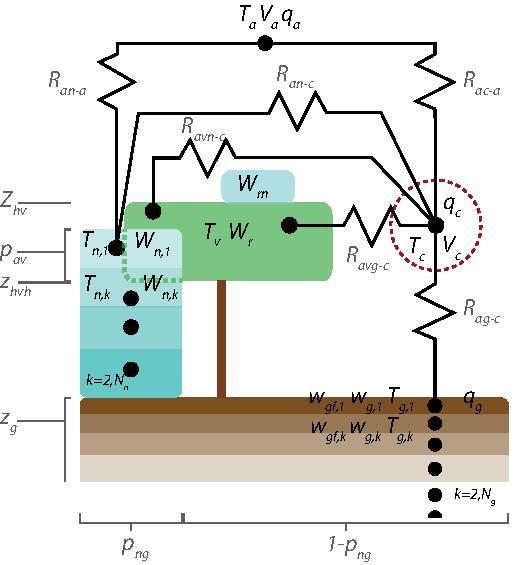
\includegraphics[angle=0, width=10cm]{\EPSDIR/schematic_g_v_ng_na_colorfill.pdf}}
\caption{
A schematic representation of 
%the composite soil-vegetation
%ISBA scheme with an explicit snowpack (ISBA-ES): left-hand side.
%The ISBA-MEB schematic is shown on the right.
the turbulent aerodynamic resistance, $R_{a}$, pathways for
ISBA-MEB. The prognostic temperature, liquid water, and liquid water
equivalent variables are shown.
The canopy air diagnostic variables are enclosed by the red-dashed circle.
The ground-based snow pack is indicated using
turquoise, the vegetation canopy is shaded green,
and ground layers are colored brown.
Atmospheric variables (lowest atmospheric 
model or observed reference level) are indicated using
the $a$ subscript.
The ground snow fraction, $p_{ng}$ (note, this corresponds to
$p_{sng}$ in the text), and canopy-snow-cover 
fraction, $p_{n\alpha}$, are indicated.
}
\label{fig:schematic_meb}
\end{figure}
%%%%%%%%%%%%%%%%%%%%%%%%%%%%%%%%%%%%%%


The surface energy budgets are formulated in terms of prognostic
equations for the temperature evolution of the bulk vegetation canopy, $T_v$, 
the snow-free ground surface (soil or litter), $T_g$, and the
ground-based
snowpack, $T_n$ (K). The prognostic hydrological variables
are: the liquid soil volumetric water content, $w_g$ (m$^3$ m$^{-3}$),
liquid water equivalent volumetric
ice content, $W_{gf}$ (m$^3$ m$^{-3}$), snow water equivalent
(SWE), $W_n$,
vegetation canopy intercepted liquid water, $W_r$, and intercepted
snow, $W_{rn}$ (kg m$^{-2}$).  
%
The diagnosed variables which are determined implicitly during the
simultaneous solution of the energy budgets are; 
%colored in dark red;
the surface specific humidity at saturation 
for each of the three energy budgets, $q$ (kg
kg$^{-1}$), and the canopy air specific humidity, $q_c$, temperature,
$T_c$ and wind speed, $V_c$ (m s$^{-1}$).
%
The surface snow cover fraction
area is represented by $p_{sng}$ as in the (baresoil part of the) 
composite version of ISBA, 
while the fraction of the canopy
buried by the ground-based snowpack is defined as $p_{\alpha n}$
%(the snow fraction parameterizations 
%are described in Section~\ref{sec:snow_frac}.)
%
%Finally, 
The snowpack has $N_n$ layers, while the number of soil
layers is defined as $N_g$ where $k$ is the vertical index (increasing
from 1 at the surface downward). The ground and snowpack uppermost
layer temperatures 
correspond to those used for the surface energy budget (i.e. $k=1$).
%

%=========================================================================================================
\subsubsection{Snow Fractions}
\label{sec:snow_frac} 
%=========================================================================================================

%Snow is known to
%have a significant impact on heat conduction fluxes owing to
%it's relatively high insulating properties. In addition, it can significantly
%reduce turbulent transfer owing to reduced surface roughness, and it
%has a relatively large surface albedo thereby impacting the surface net
%radiation budget. Thus, the parameterization of it's areal coverage
%turns out to be a critical aspect of LSM modeling of snowpack-atmosphere
%interactions and sub-surface soil and hydrological processes. 
%
The fractional ground coverage by the snowpack, $p_{sng}$, 
is defined from Eq.~\ref{eq:isba_snow_frac_ground}.
%
%%%%%%%%%%%%%%%%%%%%%%%%%
%\begin{equation}
%\label{eq:meb_png}
%p_{sng} = W_n/W_{n,crit}
%\hskip1.in
%\left( 0 \leq p_{sng} \leq 1 \right)
%\end{equation}
%%%%%%%%%%%%%%%%%%%%%%%%%
%
%where currently 
The suggested value for the critical snow water equivalent (at which
coverage is unity) for MEB
is currently $W_{crn}=1$ (kg m$^{-2}$).
Note that this is considerably lower than the previous value of 10 kg m$^{-2}$
used in ISBA 
(Douville et al., 1995)
\nocite{DOUVILLE1995a}, 
but this value has been shown to improve the ground soil
temperatures  using an explicit snow scheme within 
ISBA 
Brun et al. (2013)\nocite{brun_2012}.

Note that for MEB, the ISBA snow fraction over vegetation, 
$p_{snv}$ (Eq.~\ref{eq:isba_snow_frac_veg}), 
is not used since it is
more consistent with a composite surface.
The fraction of the vegetation canopy which is buried by ground-based snow
which is deamed to be more consistent with a forest canopy structure
is defined as 
%
%%%%%%%%%%%%%%%%%%%%%%%%%
\begin{equation}
\label{eq:meb_LAIcansnow}
p_{n\alpha} = 
\frac
{\left(D_n - z_{hv,b}\right)}
{\left(z_{hv} - z_{hv,b}\right)}
\hskip1.25in
\left( 0 \leq  p_{n\alpha} \leq 1\right)
\end{equation}
%%%%%%%%%%%%%%%%%%%%%%%%%
%
where $D_n$ is the total ground-based snowpack depth (m), 
%$z_{hv}$ is defined as the top of the vegetation canopy (m), 
and $z_{hvb}$
represents the base of the vegetation canopy (m) 
(see Fig.~\ref{fig:forest_snow_MEB}) which is currently defined as
%
%%%%%%%%%%%%%%%%%%%%%%%%%%
\begin{equation}
\label{eq:meb_pn_alphan}
z_{hvb} = a_{hv}\,\left(z_{hv} - z_{hv,min}\right)
\hskip1.in
\left(z_{hvb} \geq 0\right)
%
\end{equation}
%%%%%%%%%%%%%%%%%%%%%%%%%%%
%
where $a_{hv}=0.2$ and the effective canopy base height is
set to $z_{hv,min}=2$ (m) for forests. The foliage distribution
should be reconsidered in further development since literature
suggests
(e.g. Massman, 1982)\nocite{Massman1982}, 
that the foliage is not
symmetrically distributed in the crown but skewed upward.



%%%%%%%%%%%%%%%%%%%%%%%%%%%%%%%%%%%%%%
%\vskip.25in
\begin{figure}[!b]
\centerline{ 
%\includegraphics[angle=0, width=12cm, clip=true, trim=1cm 7cm 1cm 8cm]{FIGURES/forest_snow_MEB_sketch.pdf}}
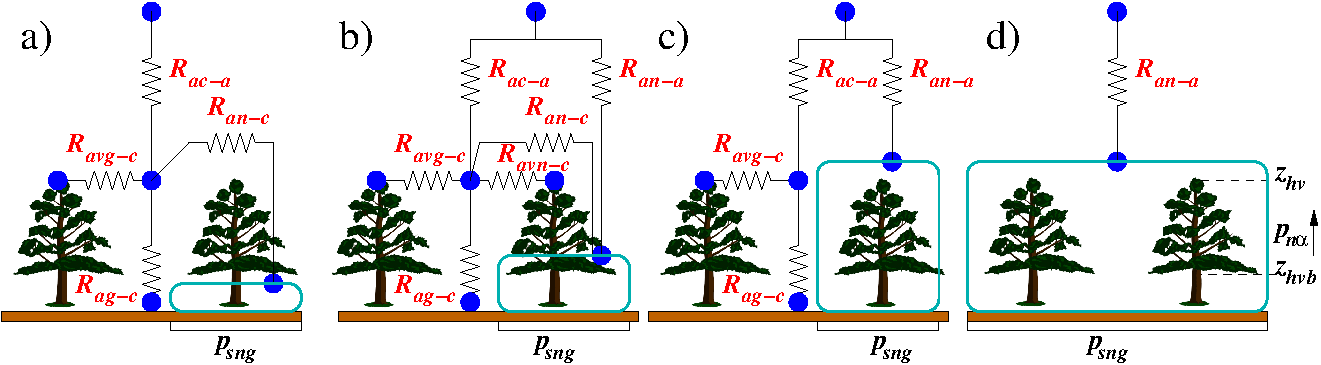
\includegraphics[angle=0, width=14cm, clip=true]{\EPSDIR/tree_resistance.pdf}}
\caption{
A schematic sketch illustrating the role of $p_{n\alpha}$, the fraction of the vegetation
canopy which is buried by ground-based snow. In panel a), the snow is well
below the canopy base, $z_{hvb}$, 
resulting in $p_{n\alpha}=0$ and the snow has no direct energy exchange with the atmosphere.
In panel b), the canopy is partly buried by snow ($0<p_{n\alpha}<1$) and the snow has energy exchanges
with both the canopy air and the atmosphere.
In panel c), the canopy is fully buried by snow ($p_{n\alpha}=1$) and the snow has energy exchange
only with the atmosphere while the soil and canopy only exchange with
the canopy air space ($p_{sng}<1$). Finally, in panel d), both
$p_{sng}=1$ and $p_{n\alpha}=1$, so
that the only exchanges are between the snow and the atmosphere.
}
\label{fig:forest_snow_MEB}
\end{figure}
%%%%%%%%%%%%%%%%%%%%%%%%%%%%%%%%%%%%%%


%=========================================================================================================
\subsubsection{Energy Budget}
\label{sec:meb_energy_budget}
%=========================================================================================================

The coupled energy budget equations for a three-source model
can be expressed for a single bulk canopy, a ground-based snowpack and a 
underlying ground surface as
%
%%%%%%%%%%%%%%%%%%%%%%%%%
\begin{align}
\label{eq:meb_cvdtvdt_three}
{\cal C}_v {\frac {\partial T_v}{\partial t}} =& 
R_{n\,v} - H_{v} - LE_{v} 
\,+\, L_f\,\Phi_{v} 
\\
%
\label{eq:meb_cgdtgdt_three}
{\cal C}_{g,1} {\frac {\partial T_{g,1}}{\partial t}} =& 
\left(1-p_{sng}\right) \left( R_{n\,g} - H_{g} - LE_{g}\right)
\,+\, p_{sng}\left(G_{gn} + \tau_{n,N_n}SW_{n\,n}\right)
\,-\, G_{g,1} \,+\, L_f\,\Phi_{g,1} 
\\
%
\label{eq:meb_cndtndt_three}
%p_{sng}\, 
{\cal C}_{n,1} {\frac {\partial T_{n,1}}{\partial t}} =& 
%\left( 
R_{n\,n} - H_{n} - LE_{n} - \tau_{n,1}SW_{n\,n} 
\,+\, \xi_{n,1} \,-\, G_{n,1} \,+\, L_f\,\Phi_{n,1} 
%\right) p_{sng} 
%
\end{align}
%%%%%%%%%%%%%%%%%%%%%%%%%
%
where $T_{g,1}$ is the uppermost ground (surface soil or litter layer) temperature,
$T_{n,1}$ is the surface snow temperature, 
and $T_v$ is the bulk-canopy temperature (K). 
%
Note that the subscript 1
indicates the uppermost layer or the base of the layer (for fluxes) 
for the soil and snowpack.
% (vegetation is
%treated as a single bulk layer, thus there is no indexing).
%$L_f$ represents the latent heat of fusion, and
%$LE$ represents the various latent heat flux terms.
%$L$ represents the effective latent heat (J kg$^{-1}$)
%(more details are given in Appendix~\ref{app:turb_flux_expressions}).
%The subscript for the turbulent fluxes is defined using the same convention
%as for aerodynamic resistances (Section~\ref{sec:model_descrip}).
%surface-atmosphere: $g-c$ implies ground to canopy
%air space, $v-c$ repsesents vagatation canopy to canopy
%air space, and $n-N$ implies snow surface to the overlying
%atmosphere (the center-level of the $N$th layer of the atmospheric model, just above the surface: we sometimes 
%also use the subscript $a$ 
%to represent this level).
%
The ground-based snow fraction is defined as $p_{sng}$. 
Note that the terms of Eq.~\ref{eq:meb_cgdtgdt_three} are multiplied by
$p_{sng}$ to make them patch-relative (or grid-box relative in the case
of single-patch mode) since the snow can potentially cover only part of the
patch. Within the snow module itself, the notion of
$p_{sng}$ is not used (the computations are snow-relative). 
%The formulation for $p_{sng}$ is described in 
%Section~\ref{sec:snow_frac}.
But note that when simultaneously solving the
coupled equations
Eq.s~\ref{eq:meb_cvdtvdt_three}-\ref{eq:meb_cndtndt_three}, 
Eq.~\ref{eq:meb_cndtndt_three} must be multiplied by $p_{sng}$ since
snow only covers a fraction
of the area to make the snow patch-relative: further details are given
in Section~\ref{sec:meb_discret_ebud}. 

The phase change terms (freezing less melting: expressed in kg m$^{-2}$ s$^{-1}$) 
terms for the snow water equivalent intercepted by the vegetation
canopy, 
the uppermost ground layer, and the uppermost snowpack layer are
represented by
$\Phi_{v}$,  $\Phi_{g,1}$ and $\Phi_{n,1}$, respectively.
$L_f$ represents the latent heat of fusion (J kg$^{-1}$).
%
The computation of $\Phi_{g,1}$ uses the Gibbs free-energy method
(also note that $\Phi_{g,1}=\Phi_{f,1}-\Phi_{m,1}$: see Section~\ref{sec:isba_soil_ice}), 
$\Phi_{n,1}$ is based on available liquid for freezing or cold
content for freezing 
(see Section~\ref{sec:isba_multi_layer_snow})
%(Boone and Etchevers, 2001)\nocite{Boone2001},
and $\Phi_{v}$ is described herein (see Eq.~\ref{eq:meb_sn2w}).
%
%$LE$ represents the various latent heat flux terms.
Note that all of the phase change terms are computed as adjustments
to the surface temperatures (after the fluxes have been computed),
therefore only the energy storage terms (and not the fluxes) 
are modified directly by phase
changes for each model time step.
%
The last term on the RHS of Eq.~\ref{eq:meb_cndtndt_three}, 
$\xi_{n,1}$, represents the effective heating or cooling
of a snowpack layer caused by exchanges in enthalpy between the
surface and sub-surface model
layers 
when the vertical grid is reset (the snow model grid layer thicknesses vary in time). 

%-----------------------------------------------------------------------------------------------------
%
%The heat capacity (J m$^{-3}$ K$^{-1}$) of each layer is expressed using $c$, while
%$D_{n,k}$ and $\Delta z_{g,k}$ represent the snow and soil layer thicknesses (m), respectively.
%The ${\cal C}$ terms represent the special case for the surface for $k=1$. 
%%They
%%are analogous to the inverse of the
%%Force-Restore thermal inertia coefficients. 
%%Note that if there is no understory vegetation, then ${\cal C}_g=c_{g,1}\Delta z_{g,1}$, while for 
%%snow, ${\cal C}_n=c_{n,1} D_{n,1}$ always. 
The surface ground, snow,
and vegetation
effective heat capacities, ${\cal C}_{g,1}$, ${\cal C}_v$ and 
${\cal C}_{n,1}$ (J m$^{-2}$ K$^{-1}$)
are defined, respectively, as
%
%The values for the soil and the vegetation are defined as
%
%%%%%%%%%%%%%%%%%%%%%%%%%
\begin{align}
\label{eq:meb_cvdtvdtn_sfc_g_hcaps}
%
{\cal C}_{g,1} = & 
\Delta z_{g,1}\, c_{g,1}\
%\frac{1}{ p_{ff}/C_f \,+\, 
%\left(1-p_{ff}\right)/
%\left( \Delta z_{g,1}\, c_{g\,i}\right)}
%
%\hskip.5in & \left( {\cal C}_{g,1} \geq {\cal C}_{g,min}\right)
%\\
%\label{eq:meb_cvdtvdtn_sfc_n_hcaps}
%
\\
\label{eq:meb_cvdtvdtn_sfc_v_hcaps}
%
{\cal C}_{v} = & C_{vb} \,+\, C_i \, W_{r,n} \,+\, C_w \, W_r
%
%& \left( {\cal C}_{v} \geq {\cal C}_{v,min}\right)
\\
\label{eq:meb_cvdtvdtn_sfc_n_hcaps}
%
{\cal C}_{n,1} = & D_{n,1}\,c_{n,1}
\end{align}
%%%%%%%%%%%%%%%%%%%%%%%%%
%
%The flooded fraction, $p_{ff}$ is discussed in more detail in
%Sect.~\ref{sec:water_budget}.
%
where
$C_i$ and $C_w$ are the specific
heat capacities for solid 
($2.106 \times 10^3$ J kg$^{-1}$ K$^{-1}$) 
and liquid water ($4.218 \times 10^3$ J kg$^{-1}$ K$^{-1}$), respectively.
%
The uppermost ground layer thickness is $\Delta z_{g,1}$ (m),
and the corresponding heat capacity of this layer is defined as
$c_{g\,1}$ (J m$^{-3}$ K$^{-1}$). 
%
%The uppermost soil layer ranges between 0.01
%and 0.03 m for most applications, so that the interactions between
%surface fluxes and fast temperature changes in the surface soil layer
%can be represented.
%
There are two options for modeling the thermal properties of the
uppermost ground layer.
%
First, they ($c_{g\,1}$ and $\lambda_{g\,1}$)
can be defined using the default ISBA configuration for a soil layer 
with parameters based on soil texture properties
which can also incorporate
the thermal effects of soil organics
(Decharme et al., 2016)\nocite{Decharme16}: see Section~\ref{sect:isbacc_soil}.
%
The second option, 
which is the default when using MEB,
is to model the uppermost ground layer as forest litter.
This means using values of $c$, $\lambda$ and $\Delta z$ 
which correspond to litter to compute ${\cal C}$
in Eq.~\ref{eq:meb_cvdtvdtn_sfc_g_hcaps}
(Napoly et al., 2017)\nocite{napoly_ea_2017}:
see Section~\ref{sec:meb_litter} for details. 
%
%See Napoly et al. (2016)\nocite{napoly_ea_2016} 
%for a detailed description of this scheme
%and it's impact on the surface energy budget.

%
%%%%%%%%%%%%%%%%%%%%%%%%%%
%\begin{equation}
%\label{eq:meb_cvdtvdtn_sfc_g_soil}
%c_{g\,i} = \left(1-w_{sat,i}\right) C_{g,i} \,+\, C_l \,\rho_l \,w_{g,i} 
%\,+\, C_i \,\rho_i \, w_{gf,i}
%%
%\end{equation}
%%%%%%%%%%%%%%%%%%%%%%%%%
%
%where $w_{g}$ and $w_{gf}$ represent the volumetric liquid water and liquid water
%equivalent soil water contents (m$^{3}$ m$^{-3}$), respectively (see Sect.\ref{sec:water_budget}
%for their governing equations). The density of liquid water and ice
%(assumed to have a constant value of 920 kg m$^{-3}$) are defined by $\rho_l$
%and $\rho_i$, respectively. The soil porosity is represented by $w_{sat}$.
%
The canopy is characterized by low heat capacity which means that its temperature responds
fast to changes in fluxes. Thus, to realistically simulate diurnal variations in 2-meter temperature
this effect must be accounted for.
Sellers et al. (1986)\nocite{Sellers86} 
defined the value as
being the heat capacity of 0.2 kg m$^{-2}$ of water per unit leaf area
index ($LAI$: m$^{2}$ m$^{-2}$). This results in values on the order of $1\times 10^{4}$ J
m$^{-2}$ K$^{-1}$ for forest canopies in general. 
%
%The canopy acts more or less
%like a cover above the ground surface, therefore, it is really the temperature and specific humidity conditions
%in the canopy air space, $T_{c}$ and $q_{c}$, that set the conditions for heat fluxes between canopy, ground surface,
%and lowest model level. 
%
For local scale simulations, $C_{vb}$ can be defined based on
observational data.
In spatially distributed simulations (or when observational data is
insufficient), $C_{vb} = 0.2/C_{V,ref}$
where the vegetation thermal
inertia, $C_{V,ref}$ is defined as a function of vegetation class by the
SURFEX default physiographic database ECOCLIMAP
(Faroux \etal, 2013)\nocite{faroux2013}. 
%
Note that $C_V$ has been determined for the composite
soil-vegetation scheme, so the factor 0.2 is used to reduce this value
to be more representative of vegetation and on the order of the
value discussed by Sellers et al. (1986)\nocite{Sellers86}.
Numerical tests have shown that using this value, the canopy
heat storage is on the order of 10 W m$^{-2}$ at mid-day for a typical
mid-latitude summer day for a forest.
%
The minimum vegetation heat capacity value is limited at
$1\times 10^{4}$ (J m$^{-2}$ K$^{-1}$)
in order to model, in a rather simple fashion, 
the thermal inertia of stems, branches, trunks, etc.
%In fact, 
%there is not much model sensitivty to this
%parameter (i.e. futher phase shifts and amplitude increases) 
%for lower values except that numerical problems can arise for large time
%steps. Thus, this value reduces the potential for oscillations or
%shocks in $T_v$, and at the same time takes into account plant biomass
%in the absence of leaves.
%
The contributions from intercepted snow and rain are incorporated,
where $W_{r,n}$ and $W_r$ (kg m$^{-2}$) represent the 
equivalent liquid water content of
intercepted canopy snow and liquid water, respectively. 
%
The uppermost snow layer thickness is $D_{n,1}$ (m), and the
corresponding heat capacity is represented by $c_{n,1}$ 
(see Section~\ref{sec:isba_multi_layer_snow} for details on the
explicit snow scheme variables).
%(Boone and Etchevers, 2001)\nocite{Boone2001}. 
%Note that $D_{n,1}$ is limited to
%values no larger than several centimeters in order to model a
%reasonable thermal inertia (i.e. in order to represent the diurnal
%cycle) in a fashion analogous to the soil.
%For more details, see 
%Decharme et al. (2016)\nocite{Decharme16}, 
%
The numerical solution of the surface energy budget,
sub-surface soil and snow temperatures, and the implicit numerical
coupling with the atmosphere is described in 
Appendix~\ref{app:meb_numerical_soln}.

%=========================================================================================================
\subsubsection{Turbulent fluxes}
\label{sec:meb_energy_budget_turb}
%=========================================================================================================

In this section, the turbulent heat and water vapor fluxes 
in Eq.s~\ref{eq:meb_cvdtvdt_three}-\ref{eq:meb_cndtndt_three} are described.

%-------------------------------------------------------------------------------------
%\subsubsection{Sensible heat fluxes}
%\label{sec:energy_budget_turb_h}



The MEB sensible heat fluxes are defined as
%
%%%%%%%%%%%%%%%%%%%%%%%%%
\begin{align}
\label{eq:meb_sens_veg}
H_{v} =& \rho_a \,
{\frac{\left( {\cal T}_v - {\cal T}_c \right)}{R_{a\,v-c}}}
\\
%
\label{eq:meb_sens_grnd}
H_{g} =& \rho_a \,
%\left(1-p_{sng}\right) \,
{\frac{\left( {\cal T}_g - {\cal T}_c \right)}{R_{a\,g-c}}} 
\\
%
\label{eq:meb_sens_snow}
H_{n} =& \rho_a \,
\left[
\left(1-p_{n\alpha}\right)
\, 
{\frac{\left( {\cal T}_n - {\cal T}_c \right)}{R_{a\,n-c}}} 
\,+\,
p_{n\alpha}
\, 
{\frac{\left( {\cal T}_n - {\cal T}_a \right)}{R_{a\,n-a}}}  
\right]
\\
%
\label{eq:meb_sens_ca}
H_{c} =& 
\rho_a \,{\frac{\left( {\cal T}_c - {\cal T}_a \right)}{R_{a\,c-a}}} 
\\
%
\label{eq:meb_sens_all}
%H =& 
%\left(1-p_{n\alpha}\, p_{sng}\right)\, H_{c}
%\,+\,
%p_{n\alpha}\, p_{sng}\, H_{n-a}
H =& \rho_a \,
\left[
\left(1-p_{n\alpha}\, p_{sng}\right)
\, 
{\frac{\left( {\cal T}_c - {\cal T}_a \right)}{R_{a\,c-a}}} 
\,+\,
p_{n\alpha}\, p_{sng}
\, 
{\frac{\left( {\cal T}_n - {\cal T}_a \right)}{R_{a\,n-a}}} 
\right]
%
\end{align}
%%%%%%%%%%%%%%%%%%%%%%%%%
%
where $\rho_a$ represents the lowest atmospheric layer average air
density (kg m$^{-3}$).
The fluxes between the canopy air space and  
the vegetation, $H_v$, the snow-free ground, $H_g$, and the ground-based
snowpack, $H_n$, 
%are defined by 
%Eq.s~\ref{eq:meb_sens_veg}-\ref{eq:meb_sens_snow}, 
%respectively.
%These fluxes 
appear in the surface energy budget equations 
(Eq.s\ref{eq:meb_cvdtvdt_three}-\ref{eq:meb_cndtndt_three}).
%
The sensible heat flux from the ground-based snowpack (Eq.~\ref{eq:meb_sens_snow}) 
is partitioned by the fraction of the vegetation which is buried by the
ground-based snowpack, $p_{n\alpha}$, 
between an exchange between the canopy air space,
%$H_{n-c}$, 
and the overlying atmosphere
(Eq.~\ref{eq:meb_LAIcansnow}).
%
The heat flux between the overlaying atmosphere and the canopy air
space is represented by $H_c$, and it is equivalent to the sum of
the fluxes between the different energy budgets and the canopy air
space.
%
The total flux exchange between the
overlying atmosphere and the surface (as seen by the atmosphere) 
is defined by $H$.
It is comprised of two components: the heat exchange between the
overlying atmosphere and the canopy air space 
and the part of the ground-based snowpack 
which is burying the vegetation.
%
%It is convenient to split $H_{n}$ into two components since one
%governs the coupling between the canopy air space and the snow
%surface, while the other modulates the exchanges with the overlying
%atmosphere (as the canopy layer becomes buried).
%
%Using 
%the definition of the total canopy resistance, $R_{a\,v-c}$ (Eq.~\ref{eq:resis}),
%the canopy heat flux, $H_v$ (Eq.~\ref{eq:sens_veg}) can be split into
%the sensible heat fluxes from the partially snow-buried and snow-free
%canopy:
%
%%%%%%%%%%%%%%%%%%%%%%%%%%
%\begin{align}
%\label{eq:sens_veg_vn}
%H_{vn} =& \rho_a \,
%\left( {\cal T}_v - {\cal T}_c \right)
%\left[
%{\frac{\left(1-p_{n\alpha}\right)\,p_{sng}}{R_{a\,vn-c}}}
%\right]
%\\
%
%\label{eq:sens_veg_vg}
%H_{vg} =& \rho_a \,
%\left( {\cal T}_v - {\cal T}_c \right)
%\left[
%{\frac{\left(1-p_{sng}\right)}{R_{a\,vg-c}}} 
%\right]
%
%\end{align}
%%%%%%%%%%%%%%%%%%%%%%%%%
%
The ground-based snowpack heat flux, $H_n$ (Eq.~\ref{eq:meb_sens_snow}), 
can be split into a part which modulates the
heat exchange
with the canopy air space, $H_{n-c}$ and the other part which 
controls the exchanges directly with the overlying atmosphere,
$H_{n-a}$, defined as
%
%%%%%%%%%%%%%%%%%%%%%%%%%%
\begin{align}
%
\label{eq:meb_sens_snow_canopy_n}
H_{n-c} =& \rho_a \,
\, 
{\frac{\left( {\cal T}_n - {\cal T}_c \right)}{R_{a\,n-c}}} 
%
\\
\label{eq:meb_sens_snow_atmos_a}
H_{n-a} =& \rho_a \,
{\frac{\left( {\cal T}_n - {\cal T}_a \right)}{R_{a\,n-a}}}  
\end{align}
%%%%%%%%%%%%%%%%%%%%%%%%%
%
${\cal T}_c$ is diagnosed by imposing conservation of the heat fluxes
between the surface and the canopy air (As described in
Appendix~\ref{app:meb_numerical_soln}).
%
Using the definition in Eq.~\ref{eq:meb_sens_snow_atmos_a},
the total sensible heat flux exchange with the atmosphere 
(Eq.~\ref{eq:meb_sens_all})
can also be written in more compact form as
%
%%%%%%%%%%%%%%%%%%%%%%%%
\begin{equation}
H = \rho_a \left[
\left(1-p_{sng}\,p_{n\alpha}\right) \, H_c
\,+\,
p_{sng}\,p_{n\alpha} \, H_{n-a}
\right]
\end{equation}
%%%%%%%%%%%%%%%%%%%%%%%%
%
%This method has been developed to model the covering of
%low vegetation canopies 
%or shrubs 
%by a ground-based snowpack.
%
%%%%%%%%%%%%%%%%%%%%%%%%%
%\begin{align}
%
%\label{eq:meb_sens_snow_canopy}
%H_{n-c} =& \rho_a \,
%\, 
%{\frac{\left( {\cal T}_n - {\cal T}_c \right)}{R_{a\,n-c}}} 
%
%\\
%\label{eq:meb_sens_snow_atmos}
%H_{n-a} =& \rho_a \,
%{\frac{\left( {\cal T}_n - {\cal T}_a \right)}{R_{a\,n-a}}}  
%\end{align}
%%%%%%%%%%%%%%%%%%%%%%%%%
%
%
%$C_p$ is the specific heat capacity of dry air (J kg$^{-1}$ K$^{-1}$),
%
Finally, the final fluxes for the given patch are aggregated using
$p_{sng}$ and $p_{n\alpha}$.
%: the full expressions are given 
%in Appendix~\ref{sensible_heat_fluxes}.


The total canopy aerodynamic resistance is comprised 
of snow-buried, $R_{a\,vn-c}$, and non-snow buried, $R_{a\,vg-c}$, 
resistances from
%
%%%%%%%%%%%%%%%%%%%%%%%%%%
\begin{equation}
\label{eq:meb_resis}
R_{a\,v-c} = 
{\left[
{\frac{\left(1-p_{n\alpha}\right)\,p_{sng}}{R_{a\,vn-c}}}
\,+\, 
{\frac{\left(1-p_{sng}\right)}{R_{a\,vg-c}}} 
\right]}^{-1}
%
\end{equation}
%%%%%%%%%%%%%%%%%%%%%%%%%%%
%
%
The separation of the resistances is done to mainly account for differences
in the roughness length between the buried and non-covered parts of
the vegetation canopy, so
the primary effect of snow cover is to increase the resistance
relative to a snow-free surface assuming the same temperature gradient
owing to a lower surface roughness, thus $R_{a\,vn-c} \geq R_{a\,vg-c}$.
%
The formulation also provides a continuous
transition to the case of vanishing canopy turbulent fluxes 
as the canopy becomes entirely buried
(as $p_{n\alpha}\rightarrow 1$).
%
In this case,
the energy budget 
equations collapse into a simple coupling
between the snow surface and the overlying atmosphere, and
the ground energy budget is simply consists in
heat conduction between the ground surface and the snowpack base.
%
%Note that the canopy aerodynamic resistance 
%$R_{a\,v-c} \rightarrow R_{a\,vg-c}$
%as $p_{n\alpha}\rightarrow 0$.
%
%
%The sensible flux between the canopy air space and the overlying
%atmosphere, $H_c$, is defined as the sum of the heat exchanges between
%the surface and the canopy air as
%
%%%%%%%%%%%%%%%%%%%%%%%%%
%\begin{equation}
%\label{eq:meb_sens_ca}
%H_{c} = p_{sng}\,H_{n-c} \,+\, \left(1-p_{sng}\right)\,H_{g}\,+\, H_{v} 
%\,\, = \,\, 
%\rho_a \,{\frac{\left( {\cal T}_c - {\cal T}_a \right)}{R_{a\,c-a}}} 
%\end{equation}
%%%%%%%%%%%%%%%%%%%%%%%%%
%
%
The formulations of the resistances between the different surfaces and
the canopy airspace and the overlying atmosphere are 
described in detail in 
Sect.~\ref{sec:meb_resistances}.
%
The canopy air temperature, which is needed by different physics
routines, 
is diagnosed
by combining Eq.~s\ref{eq:meb_sens_veg}-\ref{eq:meb_sens_all}
and solving for ${\cal T}_c$ and using
Eq.~\ref{eq:meb_thermo_var} to determine $T_c$
(see Eq.~\ref{eq:meb_canopy_air_t_update}).
%(see Appendix~\ref{app:thermo_var} for details).
%
%Finally, the total sensible heat flux exchange with the atmosphere is 
%defined as
%
%%%%%%%%%%%%%%%%%%%%%%%%%
%\begin{equation}
%\label{eq:meb_sens_all}
%H = 
%\left(1-p_{n\alpha}\, p_{sng}\right)\, H_{c}
%\,+\,
%p_{n\alpha}\, p_{sng}\, H_{n-a}
%
%H =& \rho_a \,
%\left[
%\left(1-p_{n\alpha}\, p_{sng}\right)
%\, 
%{\frac{\left( {\cal T}_c - {\cal T}_a \right)}{R_{a\,c-a}}} 
%\,+\,
%p_{n\alpha}\, p_{sng}
%\, 
%{\frac{\left( {\cal T}_n - {\cal T}_a \right)}{r_{a\,n-a}}} 
%\right]
%
%\end{equation}
%%%%%%%%%%%%%%%%%%%%%%%%%

The thermodynamic variable (${\cal T}$: J kg$^{-1}$) is linearly related to temperature as
%
%%%%%%%%%%%%%%%%%%%%%%%%%%
\begin{equation}
\label{eq:meb_thermo_var}
{\cal T}_x = {\cal B}_{x} \,+\, {\cal A}_{x} \, T_x
%
\end{equation}
%%%%%%%%%%%%%%%%%%%%%%%%%%%
%
where $x$ corresponds to one of the three surface
temperatures, canopy air temperature, $T_c$, or the overlying
atmospheric temperature, $T_a$.
The definitions of ${\cal A}_{x}$ and ${\cal B}_{x}$ depend on the
atmospheric variable in the turbulent diffusion scheme and are usually
defined to cast ${\cal T}$ in the form of dry static energy,
or potential temperature and are determined by the 
atmospheric model in coupled mode.
% (see Appendix~\ref{app:thermo_var}).
%
If potential temperature is used as the thermodynamic
variable in the coupled model diffusion scheme, then the thermodynamic
variable
%, ${\cal T}$ (J kg$^{-1}$: see
%Eq.s~\ref{eq:meb_sens_veg}-\ref{eq:meb_sens_all})
coefficients are defined as
%
%%%%%%%%%%%%%%%%%%%%%%%%%
\begin{align}
\label{eq:meb_thermo_entrophy_ax}
{\cal B}_{x} =& 0            \hskip1.2in \left(x=v,g,n,c,a\right) 
\\
\label{eq:meb_thermo_entrophy_bx}
{\cal A}_{x} =& C_p/\Pi_s    \hskip1.0in \left(x=v,g,n,c\right) 
\\
\label{eq:meb_thermo_entrophy_ba}
{\cal A}_{a} =& C_p/\Pi_a    
%
\end{align}
%%%%%%%%%%%%%%%%%%%%%%%%%
%
where $\Pi$ is the non-dimensional Exner function and $C_p$ is the heat capacity of
dry air (J kg$^{-1}$ K$^{-1}$).
If the atmospheric variable being diffused is dry static
energy then
%
%%%%%%%%%%%%%%%%%%%%%%%%%
\begin{align}
\label{eq:meb_thermo_drystatice_ax}
{\cal B}_{x} =& 0            \hskip1.2in \left(x=v,g,n,c\right) 
\\
\label{eq:meb_thermo_drystatice_aa}
{\cal B}_{a} =& g\,z_a            
\\
\label{eq:meb_thermo_drystatice_bx}
{\cal A}_{x} =& C_p       \hskip1.0in \left(x=v,g,n,c,a\right) 
%
\end{align}
%%%%%%%%%%%%%%%%%%%%%%%%%
%
where $z_a$ is the height (m) of the simulated or observed overlying
atmospheric temperature, $T_a$ and $g$ is the gravitational constant.
The choice of the atmospheric thermodynamic variable is 
transparent to ISBA-MEB (it is made within the surface-atmosphere
coupler). The default (in offline mode and in in-line mode with certain
atmospheric models) is using Eq.s~\ref{eq:meb_thermo_entrophy_ax}-\ref{eq:meb_thermo_entrophy_ba}.
Note that the method can be extended to use the actual air heat
capacity (including water vapor) if a linearization of the heat capacity is used.

%----------------------------------------------------------------------------------------
%MEB Water vapor fluxes
%----------------------------------------------------------------------------------------

The MEB water vapor fluxes 
are expressed as
%
%%%%%%%%%%%%%%%%%%%%%%%%%
\begin{align}
\label{eq:meb_evap_veg}
E_{v} =& \rho_a \, h_{sv} \,
{\frac{\left( q_{sat\,v} - q_c \right)}{R_{a\,v-c}}}
%\left[
%\chi_{vf}\, 
%{\frac{L_s}{{L}}}
%\,+\,
%\left(1-\chi_{vf}\right)
%{\frac{L_v}{{L}}}
%\right]
\\
%
\label{eq:meb_evap_grnd}
E_{g} =& 
%\rho_a \, {\frac{\left( h_{sg}\,q_{sat\,g} - h_a\, q_c\right)}
%{r_{a\,g-c}}} = 
%{\frac{\left(1-p_{sng}\right)}{r_{a\,g-c}}} 
\rho_a \, 
{\frac{\left(q_g - q_c \right)}{R_{a\,g-c}}}
%\bigg\lbrace
%h_{g}\,
%\left[ h_{ug} \, q_{sat}\left(T_g\right) - q_c \right]
%\left(1-\chi_{gf}\right) 
%{\frac{L_v}{{L}}}
%\,+\,
%h_{gf}\,
%\left( q_g - q_c \right)
%\chi_{gf} 
%{\frac{L_s}{{L}}}
%\bigg\rbrace
\\
%
\label{eq:meb_evap_snow}
E_{n}=& 
%\left(1-p_{n\alpha}\right)\,E_{n-c} \,+\, p_{n\alpha}\,
%E_{n-a}
\rho_a \, h_{sn}\,
\left[
\left(1-p_{n\alpha}\right)\,
{\frac{\left( q_{sati\,n}- q_c \right)}{R_{a\,n-c}}}
\,+\,
p_{n\alpha}\,
{\frac{\left( q_{sati\,n} - q_a \right)}{R_{a\,n-a}}}
\right]
%
%%\left[{\frac{\chi_n L_s + \left(1-\chi_n\right)L_v}
%%{{L}}}\right]
%%\bigg\lbrack
%\left[
%\left(1-p_{n\alpha}\right)\,
%{\frac{\left( q_{sati\,n}- q_c \right)}{r_{a\,n-c}}} 
% \,+\,
%p_{n\alpha}\, 
%{\frac{\left( q_{sati\,n} - q_a \right)}{r_{a\,n-a}}} 
%\right]
%%\bigg\rbrack
%%{\frac{L_s}{{L}}}
%%{\frac{{L}_n}{{L}}}
%%\,\,=\,\, E_{n-c} \,+\, E_{n-a} 
%
\\
%
\label{eq:meb_evap_ca}
E_{c} =& 
%p_{sng}\,E_{n-c} \,+\, \left(1-p_{sng}\right)\,E_{g}\,+\, E_{v} 
%\,\, = \,\, 
\rho_a \,{\frac{\left( q_c - q_a \right)}{R_{a\,c-a}}} 
%
\\
%
\label{eq:meb_evap_all}
E =& 
\rho_a \, 
\left[
\left(1-p_{n\alpha}\, p_{sng}\right)\, 
{\frac{\left( q_c - q_a \right)}{R_{a\,c-a}}} 
\,+\,
p_{n\alpha}\, p_{sng}\, 
h_{sn}\,
{\frac{\left( q_{sati\,n} - q_a \right)}{R_{a\,n-a}}}
\right]
%
%
%
%{\frac{{L}_n}{{L}}}
%{\frac{L_s}{{L}}}
%\,\,=\,\, E_{c-a} \,+\, p_{sng}\,E_{n-a} 
%
\end{align}
%%%%%%%%%%%%%%%%%%%%%%%%%
%
where, in an analogous fashion to the sensible heat flux, 
the vapor
flux between the canopy air space and the vegetation canopy, $E_v$, 
the snow-free ground, $E_g$, and the ground-based snowpack, $E_n$,
correspond to the fluxes in the surface energy budgets
(Eq.s~\ref{eq:meb_cvdtvdt_three}-\ref{eq:meb_cndtndt_three}).
The vapor flux between the canopy air and the overlying atmosphere is
represented by $E_c$, 
and the total vapor flux exchanged with the overlying
atmosphere is defined as $E$.
%
%%%%%%%%%%%%%%%%%%%%%%%%%
%\begin{align}
%\label{eq:meb_evap_snow_canopy}
%E_{n-c} =& \rho_a \, 
%h_{sn}\,
%{\frac{\left( q_{sati\,n}- q_c \right)}{R_{a\,n-c}}} 
%\\
%%
%\label{eq:meb_evap_snow_atmos}
%E_{n-a} =& \rho_a \, 
%h_{sn}\,
%{\frac{\left( q_{sati\,n} - q_a \right)}{R_{a\,n-a}}}
%\\
%\label{eq:meb_evap_ca_x}
%E_{c} =& p_{sng}\,E_{n-c} \,+\, \left(1-p_{sng}\right)\,E_{g}\,+\, E_{v} 
%\,\, = \,\, 
%\rho_a \,{\frac{\left( q_c - q_a \right)}{R_{a\,c-a}}} 
%\\
%%
%\label{eq:meb_evap_all_x}
%E =& 
%\left(1-p_{n\alpha}\, p_{sng}\right)\, E_{c}
%\,+\,
%p_{n\alpha}\, p_{sng}\, E_{n-a}
%{\frac{{L}_n}{{L}}}
%{\frac{L_s}{{L}}}
%\,\,=\,\, E_{c-a} \,+\, p_{sng}\,E_{n-a} 
%
%\end{align}
%%%%%%%%%%%%%%%%%%%%%%%%%
%
%The frozen fractions of the water in the uppermost
%ground and the vegegtation canopy, 
%are represented by 
%$\chi_{gf}$ and $\chi_{vf}$, respectively. 
%
The specific humidity (kg kg$^{-1}$) of the overlying
atmosphere is represented by $q_a$, while $q_{sat}$ and $q_{sati}$
represent the specific
humidity at saturation over liquid water and ice, respectively.
%, as a
%function of the surface pressure and temperature given in
%parentheses. 
For the surface specific humidities at saturation,
the convention $q_{sat\,x} = q_{sat}\left(T_x\right)$ is used.
%(as was done for ${\cal T}$ in Eq.~\ref{eq:meb_thermo_var}).
%
%%%%%%%%%%%%%%%%%%%%%%%%%
%\begin{align}
%\label{eq:meb_evap_snow_nc}
%E_{n-c} =& \rho_a \, 
%\left(1-p_{n\alpha}\right)\, h_{sn}\,
%{\frac{\left( q_{sati\,n}- q_c \right)}{r_{a\,n-c}}} 
%\\
%\label{eq:meb_evap_snow_na}
%E_{n-a} =& \rho_a \, 
%p_{n\alpha}\, h_{sn}\,
%{\frac{\left( q_{sati\,n} - q_a \right)}{r_{a\,n-a}}} 
%
%\end{align}
%%%%%%%%%%%%%%%%%%%%%%%%%
%
The canopy air specific humidity, $q_c$, is diagnosed
%by solving Eq.~\ref{eq:meb_evap_ca} (conservation of the mass fluxes)
%for $q_c$.
%
assuming that $E_c$ is balanced by the vapor fluxes between the canopy
air and each of the three surfaces considered
(the methodology for diagnosing the canopy air thermal properties is
described in Appendix~\ref{app:meb_numerical_soln}, 
Section~\ref{sec:meb_get_qc_and_tc}).
The effective ground specific humidity is defined as
%
%%%%%%%%%%%%%%%%%%%%%%%%%%
\begin{equation}
\label{eq:meb_q_ground}
%
q_{g} = h_{sg} \, q_{sat\,g} \,+\, \left(1+h_a\right) q_c
%
\end{equation}
%%%%%%%%%%%%%%%%%%%%%%%%%%
%
where the so-called humidity factors are defined as
%
%%%%%%%%%%%%%%%%%%%%%%%%%
\begin{align}
\label{eq:meb_hg_ground}
%
h_{sg} =& 
%\left(1-p_{sng}\right) \left[
\delta_{g} \, h_{ug}\, \left(1-\delta_i\right) 
\left({\frac{L_v}{L}}\right)
\,+\, 
\delta_{gf} \, h_{ugf}\, \delta_i \left({\frac{L_s}{L}}\right)
%\right]
%{\frac{1}{\left(1-p_n\right)}}
\\
\label{eq:meb_ha_ground}
h_a =& 
%\left(1-p_{sng}\right) \left[
\delta_{g} \, \left(1-\delta_i\right) 
\left({\frac{L_v}{L}}\right)
\,+\, 
\delta_{gf} \, \delta_i \left({\frac{L_s}{L}}\right)
%\right]
%{\frac{1}{\left(1-p_n\right)}}
%
\end{align}
%%%%%%%%%%%%%%%%%%%%%%%%%
%
The fraction of the surface layer which is frozen, $\delta_i$, is simply
defined as the ratio of the liquid water equivalent ice content to the
total water content (Eq.~\ref{eq:isba_soil_froz_frac}).


The latent heats of sublimation and vaporization are defined as $L_s$ and $L_v$
(J kg$^{-1}$), respectively.
The average latent heat, ${L}$,
is essentially a normalization factor which ranges between $L_s$ and
$L_v$ as a function of snow cover and surface soil ice.
It could be determined in a number of ways.
This coefficient ensures conservation of mass between the different
surfaces and the atmosphere.
%
One possible method is to diagnose it 
by inverting the equation for $LE_c$
(multiplying Eq.~\ref{eq:meb_evap_ca} by $L$ thereby eliminating it from
the RHS of this equation, and then solving for $L$),
but the resulting equation is difficult to apply since the terms can be either
positive or negative, and division by a small number is possible.
Here, a more smooth (in time) function is proposed which accounts for
each of the surfaces weighted by it's respective fraction:
%
%
%%%%%%%%%%%%%%%%%%%%%%%%%%
\begin{equation}
\label{eq:meb_latent_heat_avg_res}
{L} = {\frac{a_{Ls} \,L_s \,+\, a_{Lv} \,L_v}
{a_{Ls} \,+\, a_{Lv}}}
\end{equation}
%%%%%%%%%%%%%%%%%%%%%%%%%%
%
where
%
%%%%%%%%%%%%%%%%%%%%%%%%%%
\begin{subequations}
\begin{align}
a_{Lv} &= \left[ \sigma_{f\,LW} \, \left(1-p_{nv}\right) \,+\,
  \left(1-p_{sng}\right)\left(1-\delta_i\right) \right]
\left(1-p_{sng}p_{n\alpha}\right)
\\
a_{Ls} &= \left[ \sigma_{f\,LW} \, p_{nv} \,+\,
  \left(1-p_{sng}\right)\, \delta_i\,+\, p_{sng} \right]
\left(1-p_{sng}p_{n\alpha}\right)
 \,+\, p_{sng}p_{n\alpha}
%
\end{align}
\end{subequations}
%%%%%%%%%%%%%%%%%%%%%%%%%%
%
In the limit as the snow totally buries the canopy vegetation, $L
\rightarrow L_s$. In contrast, for snow and surface ice free conditions, $L=L_v$.
$\sigma_{f\,LW}$ is a normalized non-dimensional coefficient 
related to vegetation density (see Eq.~\ref{eq:meb_sigma_f_lw}).


The soil coefficient $\delta_{g}$ in Eq.s~\ref{eq:meb_hg_ground}-\ref{eq:meb_ha_ground}
is defined as
%
%%%%%%%%%%%%%%%%%%%%%%%%%%
\begin{equation}
\label{eq:meb_resis_grnd_delta_g}
%
\delta_{g} = \left({\frac{R_{a\,g-c}}
{R_{a\,g-c} \,+\, R_g}}\right) \, \delta_{gcor}
%
\end{equation}
%%%%%%%%%%%%%%%%%%%%%%%%%%
%
where the soil resistance, $R_g$, is defined by Eq.~\ref{eq:meb_resis_grnd}.
Note that the composite version of ISBA did not include an explicit
soil resistance term, so this also represents a new addition to the model.
This term was found to further improve results for baresoil evaporation
within MEB, and it's inclusion is consistent with other similar
multi-source models 
(e.g. Xue et al., 1991)\nocite{Xue91}.
%See Sect.~\ref{sec:resistances} for further details.
%
The delta function, $\delta_{gcor}$, 
is a numerical correction term 
%from ISBA 
which is
required owing to the linearization of $q_{sat\,g}$
and is unity unless both $ h_{ug}\, q_{sat\,g}< q_c$ and
$q_{sat\,g} > q_c$, in which case it is set to zero. 
%
The surface ground humidity factor is defined using the standard ISBA
formulation from Noilhan and Planton (1989)\nocite{Noilhan1989}.
%as
%
%%%%%%%%%%%%%%%%%%%%%%%%%% 
%\begin{equation}
%\label{eq:meb_soil_sfc_hg}
%h_{ug} = {\frac{1}{2}}
%\left[
%1 \,-\, {\textrm{cos}}\left( 
%{\frac{w_{g,1}}{w_{fc,1}^\ast}} \pi
%\right)\right]
%\hskip1.in \left(0 \leq h_{ug} \leq 1 \right)
%\end{equation}
%%%%%%%%%%%%%%%%%%%%%%%%%%
%
%In the case of condensation ($q_{sat\,g} < q_a$), $h_{ug}=1$
%\citeauthor{mahfouf_noilhan_91}, \citeyear{mahfouf_noilhan_91}, for details).
%%
%The effective field capacity, $w_{fc,1}^\ast$ is computed relative to
%the liquid water content of the uppermost soil layer (it is adjusted
%in the presence of soil ice compared to the default field capacity).
%The analogous form holds for the humidity factor over the
%frozen part of the surface soil layer, $h_{ugf}$,
%with $w_{g,1}$ and $w_{fc,1}^\ast$
%replaced by $w_{gf,1}$ and $w_{fcf,1}^\ast$ (m$^3$ m$^{-3}$) 
%in Eq.~\ref{eq:meb_soil_sfc_hg}, respectively
%\citep{boone_ea_00}.
%
%$\chi_{nf}$ 
Note that it would be more accurate to use $q_{sati}$ in place of
$q_{sat}$ for the sublimation of the canopy-intercepted snow and the soil ice 
in Eq.s~\ref{eq:meb_evap_veg}-\ref{eq:meb_evap_grnd}, respectively,
but this complicates the linearization and this has been neglected for now.
%The average latent heat for the snow surface is defined simply as
%${L}_n = \chi_{nf} L_s + \left(1-\chi_{nf}\right)L_v$.
%Note that when liquid is present in the uppermost snow layer, the
%temperature of the snowpack is at the freezing point, 
%thus $q_{sati}$ can be used for both liquid and solid water states
%in Eq.~\ref{eq:meb_evap_snow}.
%
The snow factor is defined as $h_{sn} = L_s/{L}$. This
factor can be modified so that $E_n$ includes both sublimation and
evaporation (Boone and Etchevers, 2000)\nocite{Boone2001},
but the impact of including a liquid water flux has been found 
to be negligible thus for simplicity, 
only sublimation is accounted for currently. 
%
%: it ranges
%in value between $L_s$ $L_v$ when snow or ground ice are present, 
%otherwise ${L}=L_v$.

%%%%%%%%%%%%%%%%%%%%%%%%%%%%%%%%%%%%%%%%%%%%%%%%%%%%%%%%%%%%%%%%%%%%%%%%%%%%%%%%%%%%%%

The leading coefficient for the canopy evapotranspiration is defined
as
%
%%%%%%%%%%%%%%%%%%%%%%%%%%
\begin{equation}
\label{eq:meb_hsv}
%
h_{sv} = \left(1-p_{nv}\right) h_{svg}\,\left(L_v/{L}\right) 
\,+\, p_{nv}\, h_{svn}\,\left(L_s/{L}\right)
%
\end{equation}
%%%%%%%%%%%%%%%%%%%%%%%%%%
%
where $ p_{nv}$ is defined by Eq.~\ref{eq:meb_rd_snowcanbeta}).
%
When part of the vegetation canopy is buried (i.e. $p_{n\alpha}>0$), 
a different roughness and $LAI$ are felt by the canopy air space so that
a new resistance is computed over the $p_{n \alpha}$ covered part of
the canopy
as is done for sensible heat flux. 
This is accounted for by defining
%
%%%%%%%%%%%%%%%%%%%%%%%%%
\begin{subequations}
\begin{align}
\label{eq:meb_h_v_n_a_svg}
%\begin{split}
%h_{svg} & = 
%p_{n}\left(1-p_{n \alpha}\right)\,\left({\frac{\varphi_{Hvn-c}}{\varphi_{Hv-c}}}\right) \,h_{vn} \,+\,
%\left(1-p_{n}\right)\left({\frac{\varphi_{Hvg-c}}{\varphi_{Hv-c}}}\right) \,h_{vg} 
%\\
%
h_{svg} =& p_{sng}\left(1-p_{n \alpha}\right)\,\left({\frac{R_{a\,v-c}}{R_{a\,vn-c}}}\right) \,h_{vn} \,+\,
\left(1-p_{sng}\right)\left({\frac{R_{a\,v-c}}{R_{a\,vg-c}}}\right) \,h_{vg} 
%\end{split}
\\
%
\label{eq:meb_h_v_n_a_svn}
h_{svn} =& 
p_{sng}\left(1-p_{n \alpha}\right)\,\left({\frac{R_{a\,v-c}}{R_{a\,vn-c}}}\right) \,+\,
\left(1-p_{sng}\right)\left({\frac{R_{a\,v-c}}{R_{a\,vg-c}}}\right) 
%
\end{align}
\end{subequations}
%%%%%%%%%%%%%%%%%%%%%%%%%
%
%and $r_{a\,vn-c}$ and $r_{a\,vg-c}$ are the resistances between the partially buried and
%totally non-buried parts of the vegetation canopy and the canopy air,
%respectively.
%and $r_{a\,v-c}=\varphi_{Hv-c}/\rho_N$.
%
The so-called Halstead coefficients in Eq.~\ref{eq:meb_h_v_n_a_svg}
are defined as
%
%%%%%%%%%%%%%%%%%%%%%%%%%
\begin{subequations}
\begin{align}
\label{eq:meb_hvg_halstead}
%
h_{vg} =& \left({\frac{R_{a\,vg-c}}{R_{a\,vg-c} + R_{s}}}\right)
\left(1-\delta\right) + \delta \,\,\,
\\
\label{eq:meb_hvn_halstead} 
h_{vn} =& \left({\frac{R_{a\,vn-c}}{R_{a\,vn-c} + R_{sn}}}\right)
\left(1-\delta\right) + \delta \,\,\,,
%
\end{align}
\end{subequations}
%%%%%%%%%%%%%%%%%%%%%%%%%
%
The stomatal resistance, $R_s$, 
can be computed using either the so-called Jarvis 
method 
%\citep{jarvis_76} described by \citet{Noilhan89} or 
or the more physically based ISBA-Ag-s method 
(the current default is AST: see Section~\ref{sec:isba_ags_options}).
%(the MEB default) 
%which includes a representation of
%photosynthesis \citep{calvet_ea_1998}.
The stomatal resistance for the partially
snow-buried portion defined as
%
%%%%%%%%%%%%%%%%%%%%%%%%%%
\begin{equation}
\label{eq:meb_rs_snow}
R_{sn} = R_s/\left[ 
1 \,-\, {\textrm{min}}\left(
p_{n \alpha}, \,\, 
1 \,-\, R_s/R_{s,max}
\right)\right]
\hskip1.5in
\left( R_{sn} \leq R_{s,max} \right)
\end{equation}
%%%%%%%%%%%%%%%%%%%%%%%%%%
%
so that the effect of coverage by the snowpack is to increase the canopy
resistance.
%The total effective Halstead
%coefficient is 
%
%%%%%%%%%%%%%%%%%%%%%%%%%%
%\begin{equation}
%\label{eq:meb_hv_halstead}
%h_{v} =\left(1-p_{n \alpha}\right) \, h_{vg} \,+\, p_{n \alpha}\,h_{vn}
%\end{equation}
%%%%%%%%%%%%%%%%%%%%%%%%%%
%
Note that when the canopy is not partially or fully 
buried by ground based snowpack ($p_{n \alpha}=0$) and
does not contain any intercepted snow ($p_{nv}=0$),
%the Halstead coefficient is $h_v=h_{vg}$ and
the leading coefficient for the canopy evapotranspiration 
simplifies to the same form as the Halstead coefficient
from the composite version of ISBA ($h_v$: Eq.~\ref{eq:isba_halstead}) as
%\citep{mahfouf_noilhan_91}
%
%%%%%%%%%%%%%%%%%%%%%%%%%
\begin{equation}
\label{eq:meb_hv}
%
h_{sv} = \left({\frac{R_{a\,vg-c}}{R_{a\,vg-c} + R_{s}}}\right)
\left(1-\delta\right) + \delta \,\,\,
\hskip1.in
\left(p_{n \alpha}=0 \,\,\, {\textrm{and}} \,\,\, p_{nv}=0\right)
%
\end{equation}
%%%%%%%%%%%%%%%%%%%%%%%%%
%
The fraction of the vegetation covered by water is $\delta$
and is described in Sect.~\ref{sec:meb_rain_interception}.
%
%The coefficient is subdivided into a transpiration part, $h^{tr}$, and into an interception part, $h^{int}$.

The evapotranspiration from the vegetation canopy, $E_v$, is comprised
of three components:
%
%%%%%%%%%%%%%%%%%%%%%%%%%
\begin{equation}
\label{eq:meb_ev_comps}
%
E_{v} = E_{tr} \,+\, E_{r} \,+\, E_{rn} 
\end{equation}
%%%%%%%%%%%%%%%%%%%%%%%%%
%
where the transpiration, evaporation from the canopy liquid water
interception store and sublimation from the canopy snow
interception store 
are represented by $E_{tr}$, $E_{r}$, and $E_{rn}$, respectively.
%
%The expressions for these fluxes are given in Appendix~\ref{app:turb_flux_expressions}.
%
Using the definitions in Eq.s~\ref{eq:meb_hsv}-\ref{eq:meb_hvn_halstead}, the
components of $E_v$ can be 
expressed as
%
%%%%%%%%%%%%%%%%%%%%%%%%%
%\begin{align}
%\label{eq:meb_ev_etr}
%%
%E_{tr} &= \rho_a \left({\frac{L_v}{L}}\right)
%\left( q_{sat\,v} - q_c \right)\,
%\left[
%{\frac{p_{sng}\left(1-p_{n\alpha}\right)}{R_{a\,vn-c}+R_{sn}}}
%\,+\, 
%{\frac{1-p_{sng}}{R_{a\,vg-c}+R_{s}}}
%\right]\, 
%\left(1-p_{nv}\right)\,\left(1-\delta\right)
%\\
%\label{eq:meb_ev_er}
%%
1%E_{r} &= \rho_a \left({\frac{L_v}{L}}\right)
%\left( q_{sat\,v} - q_c \right)\,
%\left[
%{\frac{p_{sng}\left(1-p_{n\alpha}\right)}{R_{a\,vn-c}}}
%\,+\, 
%{\frac{1-p_{sng}}{R_{a\,vg-c}}}
%\right]\, 
%\left(1-p_{nv}\right) \, \delta \,
%\\
%\label{eq:meb_ev_evn}
%%
%E_{rn} &= \rho_a \left({\frac{L_s}{L}}\right)
%\left( q_{sat\,v} - q_c \right)\,
%\left[
%{\frac{p_{sng}\left(1-p_{n\alpha}\right)}{R_{a\,vn-c}}}
%\,+\, 
%{\frac{1-p_{sng}}{R_{a\,vg-c}}}
%\right]\, 
%p_{nv}
%
%\end{align}
%%%%%%%%%%%%%%%%%%%%%%%%%
%%%%%%%%%%%%%%%%%%%%%%%%%
\begin{align}
\label{eq:meb_ev_etr}
%
E_{tr} &= \rho_a \left({\frac{L_v}{L}}\right)
\left( q_{sat\,v} - q_c \right)\,
\left[
{\frac{p_{sng}\left(1-p_{n\alpha}\right)}{R_{a\,vn-c}+R_{sn}}}
\,+\, 
{\frac{1-p_{sng}}{R_{a\,vg-c}+R_{s}}}
\right]\, 
\left(1-p_{nv}\right)\,\left(1-\delta\right)
\\
\label{eq:meb_ev_er}
%
E_{r} &= \rho_a \left({\frac{L_v}{L}}\right)
\left( q_{sat\,v} - q_c \right)\,
\left[
{\frac{p_{sng}\left(1-p_{n\alpha}\right)}{R_{a\,vn-c}}}
\,+\, 
{\frac{1-p_{sng}}{R_{a\,vg-c}}}
\right]\, 
\left(1-p_{nv}\right) \, \delta \,
\\
\label{eq:meb_ev_evn}
%
E_{rn} &= \rho_a \left({\frac{L_s}{L}}\right)
\left( q_{sat\,v} - q_c \right)\,
\left[
{\frac{p_{sng}\left(1-p_{n\alpha}\right)}{R_{a\,vn-c}}}
\,+\, 
{\frac{1-p_{sng}}{R_{a\,vg-c}}}
\right]\, 
p_{nv}
%
\end{align}
%%%%%%%%%%%%%%%%%%%%%%%%%
%
The complex resistances (bracketed terms in 
Eq.s~\ref{eq:meb_ev_etr}-\ref{eq:meb_ev_evn}) 
arise owing to the
inclusion of the effects of burying the snow canopy by the ground
based snowpack. If the ground-based snowpack is not sufficiently deep
to bury any of the canopy ($p_{n\alpha}=0$),
then the bracketed term in Eq.~\ref{eq:meb_ev_etr} simplifies 
to $1/\left(R_{a\,vg-c} + R_s\right)$
(note that $R_{a\,vg-c}=R_{a\,v-c}$ when $p_{n\alpha}=0$ from
Eq.~\ref{eq:meb_resis}),
and likewise
the bracketed terms in Eq.s~\ref{eq:meb_ev_er}-\ref{eq:meb_ev_evn} 
simplify to $1/R_{a\,vg-c}$.
%
Finally, the partitioning between the vapor fluxes from intercepted
snow and the snow-free canopy reservoir and transpiration is done
using $p_{nv}$.
%, which represents the fraction of the snow interception
%reservoir which is filled (see Eq.~\ref{eq:meb_rd_snowcanbeta}).



Using the definitions of $q_g$ from Eq.~\ref{eq:meb_q_ground}
together with those for the humidity factors, $h_{sg}$ and $h_a$
(Eq.s~\ref{eq:meb_hg_ground} and \ref{eq:meb_ha_ground}, respectively) and
the soil coefficient, $\delta_g$ (Eq.~\ref{eq:meb_resis_grnd_delta_g}),
the bare soil evaporation, $E_g$, components can be 
expressed as
%
%%%%%%%%%%%%%%%%%%%%%%%%%
\begin{align}
\label{eq:meb_eg_l}
%
E_{gl} &= \rho_a \, \left({\frac{L_v}{L}}\right) \,
\left(  h_{ug}\,q_{sat\,g} - q_c \right)
\left({\frac{\delta_{gcor}}{R_{a\,g} + R_g}}\right)
\, \left(1-\delta_i\right)
\\
\label{eq:meb_eg_f}
%
E_{gf} &= \rho_a \, \left({\frac{L_s}{L}}\right) \,
\left(  h_{ugf}\,q_{sat\,g} - q_c \right)
\left({\frac{\delta_{gfcor}}{R_{a\,g} + R_{gf}}}\right)
\, \delta_i
%
\end{align}
%%%%%%%%%%%%%%%%%%%%%%%%%%%%%%%%%%%%%%%%%%%
%
where $E_g = E_{gl} + E_{gf}$.
The delta function, $\delta_{gfcor}$, 
is a numerical correction term 
%from ISBA 
which is
required owing to the linearization of $q_{sat\,g}$
and is unity unless both $ h_{ugf}\, q_{sat\,g}< q_c$ and
$q_{sat\,g} > q_c$, in which case it is set to zero. 
%
Note that the ground resistances, $R_g$ and $R_{gf}$, are set to zero if the
forest litter option is active (the default for forests). 
%

The ground-based snowpack sublimation, $E_n$ (Eq.~\ref{eq:meb_evap_snow}), 
can be partitioned into a
vapor exchange
with the canopy air space, $E_{n-c}$ and the overlying atmosphere,
$E_{n-a}$, as
%
%%%%%%%%%%%%%%%%%%%%%%%%%
\begin{align}
\label{eq:meb_subl_eg_l}
%
E_{n-c} &= \rho_a \, \left({\frac{L_s}{L}}\right)\,
%\left( q_{sati\,n} - q_c \right)
\left({\frac{q_{sati\,n} - q_c}
{R_{a\,n-c}}}\right)
%\, \left(1-p_{n\,\alpha}\right) 
\\
\label{eq:meb_subl_eg_f}
%
E_{n-a} &= \rho_a \, \left({\frac{L_s}{L}}\right)\,
%\left( q_{sati\,n} - q_a \right)
\left({\frac{q_{sati\,n} - q_a}
{R_{a\,n-a}}}\right)
%\, p_{n\,\alpha}
%
\end{align}
%%%%%%%%%%%%%%%%%%%%%%%%%%%%%%%%%%%%%%%%%%%
%
The corresponding latent heat fluxes can be determined by simply
multiplying Eq.~\ref{eq:meb_ev_etr}-\ref{eq:meb_eg_f} by $L$.
%
Finally, using the definition in Eq.~\ref{eq:meb_subl_eg_f},
the total vapor exchange with the atmosphere 
(Eq.~\ref{eq:meb_evap_all})
can also be written in more compact form as
%
%%%%%%%%%%%%%%%%%%%%%%%%
\begin{equation}
E = \rho_a \left[
\left(1-p_{sng}\,p_{n\alpha}\right) \, E_c
\,+\,
p_{sng}\,p_{n\alpha} \, E_{n-a}
\right]
\end{equation}
%%%%%%%%%%%%%%%%%%%%%%%%



%=========================================================================================================
\subsubsection{Radiative fluxes}
\label{sec:meb_energy_budget_rad}
%=========================================================================================================

The $R_n$ terms in Eq.s~\ref{eq:meb_cvdtvdt_three}-\ref{eq:meb_cndtndt_three}
represent the surface net radiation terms (longwave and shortwave
components):
%
%%%%%%%%%%%%%%%%%%%%%%%%%%
\begin{equation}
\label{eq:meb_net_rad}
{R}_{n\,x} = SW_{net,x} \,+\, LW_{net,x} 
%
\end{equation}
%%%%%%%%%%%%%%%%%%%%%%%%%%%
%
where $x=n,g$ or $v$.
The total net radiation of the surface is
%
%%%%%%%%%%%%%%%%%%%%%%%%%%
\begin{equation}
\label{eq:meb_net_rad}
{R}_{n} = {R}_{n\,n} \,+\,{R}_{n\,g} \,+\,{R}_{n\,v} \,\,=\,
SW\downarrow \,-\, SW\uparrow \,+\,
LW\downarrow \,-\, LW\uparrow 
%
\end{equation}
%%%%%%%%%%%%%%%%%%%%%%%%%%%
%
where 
the total down-welling solar (shortwave) and atmospheric (longwave)
radiative fluxes (W m$^{-2}$) at the top of the canopy or snow surface (in the
case snow is burying the vegetation) 
are represented by $SW\downarrow$ and $LW\downarrow$, respectively.
The total
upwelling (towards the atmosphere) shortwave and longwave
radiative fluxes, $SW\uparrow$ and $LW\uparrow$, respectively,
are simply defined as the downward components 
%above the canopy and snowpack 
less the total surface net radiative fluxes (summed over the
three surfaces). 
%
The effective total surface albedo
and surface radiative temperature (and emissivity) can then be
diagnosed 
%(see the Sect.~\ref{sec:lw_radiation}) 
for coupling with the
host atmospheric model.
%
The $\tau_{n}$ is defined as the solar radiation transmission at the base of a snowpack layer, so
that $\tau_{n,1} SW_{n\,n}$ term in Eq.~\ref{eq:meb_cndtndt_three} 
corresponds the amount of shortwave radiation which is not absorbed in the uppermost snowpack layer.
For sufficiently thin snowpack, solar energy penetrating the snow to
the underlying ground surface is
expressed as  $\tau_{n,N_n} SW_{n\,n}$, where $N_n$ represents the
number of modeled snowpack layers (for a deep snowpack, this term becomes negligible).

%----------------------------------------------------------------------------------------
%MEB Shortwave radiation
%\label{sec:sw_radiation}
%----------------------------------------------------------------------------------------

%The shortwave radiation scheme is based on a plane-parallel surface (analagous to the atmosphere).
%The model considers 2 reflections with 3 reelfcting surfaces (ground, 
%ground-based snowpack and the vegetation canopy).
%
The total land surface shortwave energy budget can be shown to satisfy
%
%%%%%%%%%%%%%%%%%%%%%%%%%
\begin{equation}
  \label{eq:meb_swup_resid}
SW\downarrow = SW_{net\,g} + SW_{net\,v} + SW_{net\,n} + SW\uparrow 
%
\end{equation}
%%%%%%%%%%%%%%%%%%%%%%%%%
%
where $SW_{net\,g}$, $SW_{net\,v}$, $SW_{net\,n}$ represent the net shortwave terms for the ground,
vegetation canopy and the ground-based snowpack.
%, and the total (global) downwelling and upwelling
%shortwave radiation fluxes are defined as $SW\downarrow$ and $SW\uparrow$, respectively.
The effective surface albedo (which may be required by the atmospheric radiation
scheme or for comparison with satellite-based data etc.) 
is diagnosed as 
%
%%%%%%%%%%%%%%%%%%%%%%%%%
\begin{equation}
  \label{eq:meb_swup_alb_total_eff}
{\overline\alpha}_s = SW\uparrow/SW\downarrow
%\hskip1.in \left( SW\downarrow > 0 \right)
%
\end{equation}
%%%%%%%%%%%%%%%%%%%%%%%%%

%
The distinction between the visible (VIS)
and near-infrared (NIR) radiation components is important 
in terms of interactions with the vegetation canopy. 
%
The shortwave radiation scheme in ISBA-MEB 
is described by Carrer et al. (2013)\nocite{carrer_ea_2013}
(hereafter refered to as CEA13 in this section): it is the radiative
scheme used for ISBA-Ags applications for photosynthesis. Note that
when using MEB, it is also used for energy budget computations for
increased consistency.

The CEA13 scheme requires the vegetation and surface albedos for 2
spectral bands (visible, $VIS$, and near-infrared, $NIR$)
The $VIS$
wavelengths range from approximately 0.3 to 0.7 $\times 10^{-6}$ m, and $NIR$
wavelengths range from approximately 0.7 to 1.4 $\times 10^{-6}$ m.
%
The vegetation albedos, $\alpha_{v,VIS}$, $\alpha_{v,NIR}$, 
and the baresoil albedos, $\alpha_{g,VIS}$, $\alpha_{g,NIR}$,
are provided by ECOCLIMAP or
prescribed within the namelist file.
%
For MEB,
the snow free surface is either baresoil or litter, which is assumed
for now, to have the same albedo as the soil. 
%
MEB is, by
default, coupled to the ISBA-ES snow scheme which includes 3 spectral
bands for the snow albedo ($VIS$, $NIR$ and $UV$): the corresponding
albedo
values for each band are diagnosed from the prognostic snow age variable
as discussed in
Decharme \etal (2016)\nocite{Decharme16}. Since CEA13 and therefore MEB currently only
considers 2 spectral bands for the soil and vegetation, the snow
albedo components for the $VIS$ and $NIR$ bands are used within MEB: this
can be changed in the future as MEB is more or less transparent to
this (it would mean updating the CEA13 scheme). 
The snow $VIS$ band albedo is used as-is, while the snow $NIR$ albedo is
simply computed as
%
%%%%%%%%%%%%%%%%%%%%%%%%%%%%%%%%%%%%%%%%%%%%%
\begin{equation}
%
\alpha_{n,NIR} = \frac{\left(\alpha_n - \omega_{VIS} \, \alpha_{n,VIS} \right)}{\omega_{NIR}}
%
\end{equation}
%%%%%%%%%%%%%%%%%%%%%%%%%%%%%%%%%%%%%%%%%%%%%
%
where $\alpha_n$ is the all-wavelength snow albedo, and the usual
spectral weights $\omega_{VIS}=0.48$ and $\omega_{NIR}=0.52$ are used.
The snow albedos are time-varying and are diagnosed at each time step
based on a snow age variable as discussed in Decharme \etal (2016)\nocite{Decharme16}. 
%
The effective surface albedo required by CEA13 is represented
by the aggregatating the snow and baresoil albedo contributions
weighted by the ground snow cover fraction, $p_{sng}$. 
%
The effective surface albedo, ${\overline\alpha}_{gn}$, components are then defined as
%
%%%%%%%%%%%%%%%%%%%%%%%%%%%%%%%%%%%%%%%%%%%%%
\begin{align}
\label{eq:albedo_sfc_vis}
{\overline\alpha}_{gn,VIS} \,\ =&\,\, p_{sng} \,\alpha_{n,VIS} \,+\, \left(1-p_{sng}\right)\alpha_{g,VIS}
\\
\label{eq:albedo_sfc_nir}
{\overline\alpha}_{gn,NIR} \,\ =&\,\, p_{sng} \,\alpha_{n,NIR} \,+\, \left(1-p_{sng}\right)\alpha_{g,NIR}
\end{align}
%%%%%%%%%%%%%%%%%%%%%%%%%%%%%%%%%%%%%%%%%%%%%
%
CEA13 computes the absortion of the shortwave radiation, $SW_{net}$,
for the vegetation and soil as
%
%%%%%%%%%%%%%%%%%%%%%%%%%%%%%%%%%%%%%%%%%%%%%
\begin{align}
SW_{net,v} \,\ =&\,\, \omega_{VIS}SW_{net,v,VIS} \,+\,  \omega_{NIR} SW_{net,v,NIR}
\\
SW_{net,g} \,\ =&\,\, \omega_{VIS}SW_{net,g,VIS} \,+\,  \omega_{NIR} SW_{net,g,NIR}
\end{align}
%%%%%%%%%%%%%%%%%%%%%%%%%%%%%%%%%%%%%%%%%%%%%
%
The multi-level transmission computations 
for direct and diffuse radiation are made, and the sum of the absorbed
radiaton is $SW_{net\,v}$.
The details of these computations are given by
Carrer et al. (2013)\nocite{carrer_ea_2013}.


The effective all-wavelength surface (below-canopy) albedo 
is defined as
%
%%%%%%%%%%%%%%%%%%%%%%%%%
\begin{equation}
  \label{eq:meb_albedo_ng_specw}
%{\overline \alpha_{gn}} = p_{sng}\,\alpha_n + \left( 1 -
%p_{sng}\right){\overline\alpha}_g
{\overline\alpha}_{gn} \,\, = \,\, 
\omega_{VIS}\,{\overline\alpha}_{gn,VIS}\,+\,  
\omega_{NIR}\,{\overline\alpha}_{gn,NIR}
%
\end{equation}
%%%%%%%%%%%%%%%%%%%%%%%%%
%
which upon substitution
of Eq.s~\ref{eq:albedo_sfc_vis}-\ref{eq:albedo_sfc_nir}.
can also be expressed as
%
%%%%%%%%%%%%%%%%%%%%%%%%%
\begin{equation}
  \label{eq:meb_albedo_ng}
%{\overline \alpha_{gn}} = p_{sng}\,\alpha_n + \left( 1 -
%p_{sng}\right){\overline\alpha}_g
{\overline\alpha}_{gn} \,\, = \,\, 
p_{sng}\,\alpha_n + \left( 1 - p_{sng}\right){\alpha}_g
%
\end{equation}
%%%%%%%%%%%%%%%%%%%%%%%%%
%
where the all-wavelength albedo for the snow, $\alpha_{n}$, 
and the ground, $\alpha_{g}$, 
are computed using the same spectral weighting.
%Two spectral bands
%are currently accounted for (visible, VIS: 400-700 m$^{-9}$, and near infra-red,
%NIR: 700-1350 m$^{-9}$), which are
%provided by either observations or ECOCLIMAP 
%$p_{sng}$ is the ground snow cover fraction, and 
%There is a recent option to
%input the all-wavelenght snow-free albedo from satellite data
%{\bf REF Carrer?}, and this value can be used to scale
%the total effective albedo and the corresponding flux components.
%
%The ground-based snow albedo, $\alpha_n$,
%is prognostic and depends on the snow grain size. 
%It currently includes up to three spectral bands
%\citep{Decharme16}, 
%however, when coupled to MEB, only the two
%aforementioned spectral
%bands are currently considered for
%consistency with the vegetation and soil.
%
Note that the flooded fraction of the gridbox uses a ground-flooded zone composite
energy budget, so to consider water surfaces the
effective snow-free ground would need to be modified to include the
surface water albedo: this will be done in future versions of SURFEX.
%
%%%%%%%%%%%%%%%%%%%%%%%%%%
%\begin{equation}
%  \label{eq:meb_swup_resid_flood}
%{\overline\alpha}_g = p_{ff} \alpha_{ff} + \left(1-p_{ff}\right)\alpha_g
%
%\end{equation}
%%%%%%%%%%%%%%%%%%%%%%%%%
%
%where $p_{ff}$ is the sub-grid flooded fraction, $\alpha_{ff}$ is the effective albedo of the flooded area,
%and $\alpha_g$ is the snow-free flood-free ground albedo.
%

%%%%%%%%%%%%%%%%%%%%%%%%%%%%%%%%%%%%%%%%%%%%%%%%
%
The net solar radiation at the surface assumes one reflection from the
vegetation back to the ground or snow surface and is defined as
%
%%%%%%%%%%%%%%%%%%%%%%%%%%%%%%%%%%%%%%%%%%%%
\begin{align}
\label{eq:swnet_n_meb}
SW_{net\,n} \,\,=&\,\, 
\hskip.38in p_{sng}\,\,\, SW\downarrow \, T_r 
\left[
1 - \alpha_n + {\overline\alpha}_{gn}\, 
{\overline\alpha}_v \left(1-T_r\right)
\right]
\left(1 \,-\, \tau_{n,N_n}\right)
\\
\label{eq:swnet_g_meb}
\begin{split}
SW_{net\,g} \,\,=&\,\, \left(1-p_{sng}\right) \, SW\downarrow \, T_r 
\left[
1 - \alpha_g + {\overline\alpha}_{gn}\, 
{\overline\alpha}_v \left(1-T_r\right)
\right] \,+\,
\\
& 
\,\, 
\hskip.38in p_{sng}\,\,\, SW\downarrow \, T_r 
\left[
1 - \alpha_n + {\overline\alpha}_{gn}\, 
{\overline\alpha}_v \left(1-T_r\right)
\right] \tau_{n,N_n}
\end{split}
%
\end{align}
%%%%%%%%%%%%%%%%%%%%%%%%%%%%%%%%%%%%%%%%%%%%
%
where 
$T_r$ (dimensionless: bound between 0 and 1)
represents the fraction of the incoming radiation transmitted through the
canopy from the multi-level vegetation radiative transfer
scheme. It depends strongly on the vegetation density via the
pontentially snow-buried $LAI_n$ (see
Eq.~\ref{eq:meb_lai_snow_modif}).
%
At this point we define the energy absorbed at the snow surface 
(see the surface energy budget equations:
Eq.s~\ref{eq:meb_cgdtgdt_three}-\ref{eq:meb_cndtndt_three})
as
%
%%%%%%%%%%%%%%%%%%%%%%%%%%%%%%%%%%%%%%%%%%%%%
\begin{equation}
\label{eq:meb_sw_snow_sfc_abs}
SW_{n\,n}= SW\downarrow \, T_r \left[
1 - \alpha_n + {\overline\alpha}_{gn}\, 
{\overline\alpha}_v \left(1-T_r\right)
\right] 
\end{equation}
%%%%%%%%%%%%%%%%%%%%%%%%%%%%%%%%%%%%%%%%%%%%%
%
Note that the total surface net shortwave energy is obtained by
summing Eq.s~\ref{eq:swnet_n_meb} and \ref{eq:swnet_g_meb} resulting in simply
%
%%%%%%%%%%%%%%%%%%%%%%%%%%%%%%%%%%%%%%%%%%%%
\begin{equation}
\label{eq:swnet_sfc_meb}
SW_{net\,s} 
\,\,=\,\, 
SW_{net\,n} + SW_{net\,g}
\,\,=\,\, 
SW\downarrow \, T_r 
\big\lbrace
1 - {\overline\alpha}_{gn} \left[
1 - \alpha_v \left(1-T_r\right)\right]
\big\rbrace 
%
\end{equation}
%%%%%%%%%%%%%%%%%%%%%%%%%%%%%%%%%%%%%%%%%%%%


If we assume that none of the shortwave radiation arriving at the
snow surface is transmitted to the ground (for sufficinetly deep
snowpack, which is often the case), 
Eq.s~\ref{eq:swnet_n_meb}-\ref{eq:swnet_g_meb} simply to
%
%%%%%%%%%%%%%%%%%%%%%%%%%%%%%%%%%%%%%%%%%%%%
\begin{align}
\label{eq:swnet_n_meb_nt}
SW_{net\,n} \,\,=&\,\, 
\hskip.38in p_{sng}\,\,\, SW\downarrow \, T_r 
\left[
1 - \alpha_n + {\overline\alpha}_{gn}\, 
{\overline\alpha}_v \left(1-T_r\right)
\right]
\,=\, p_{sng}\, SW_{n\,n}
\\
\label{eq:swnet_g_meb_nt}
SW_{net\,g} \,\,=&\,\, \left(1-p_{sng}\right) \, SW\downarrow \, T_r 
\left[
1 - \alpha_g + {\overline\alpha}_{gn}\, 
{\overline\alpha}_v \left(1-T_r\right)
\right] 
%
\end{align}
%%%%%%%%%%%%%%%%%%%%%%%%%%%%%%%%%%%%%%%%%%%%


Note that for snow-free conditions, $SW_{net\,n}=0$,
${\overline\alpha}_{gn} = \alpha_g$, and
${\overline\alpha}_v = \alpha_v$, and
 so that
%
%%%%%%%%%%%%%%%%%%%%%%%%%%%%%%%%%%%%%%%%%%%%
\begin{equation}
SW_{net\,g} \,\,=\,\, SW\downarrow \, T_r 
\big\lbrace
1 - \alpha_g \left[
1 - \alpha_v \left(1-T_r\right)\right]
\big\rbrace 
%
\end{equation}
%%%%%%%%%%%%%%%%%%%%%%%%%%%%%%%%%%%%%%%%%%%%
%
so in this case, as $LAI\rightarrow 0$, $T_r\rightarrow 1$ so that
$SW_{net\,g} \rightarrow SW\downarrow \left( 1 -\alpha_g\right)$
%therefore ${\overline\alpha}_s\rightarrow\alpha_g$,
thus the net radiation collapses in the limit of vanishing vegetation
to that of a baresoil patch. 
%If ground-based snow cover is present, then the net energy is
%paritioned between $SW_{net\,g}$ and $SW_{net\,n}$.
If the surface is totally snow covered
and the vegetation is totally buried by snow, then
${\overline\alpha}_{gn}=\alpha_n$, 
and the ground net shortwave energy 
is simply $SW_{net\,g} = \tau_{n,N_n}SW\downarrow \left(1-\alpha_n\right)$ 
and the surface net shortwave energy is
$SW_{net} = SW_{net\,n} = SW\downarrow \left(1-\alpha_n\right) \left(1- \tau_{n,1}\right)$.
%
Note that the total effective albedo
(when averaged over daylight hours) is bounded by the maximum and
minimum of the prescribed soil and vegetation and prognostic
snow all-wavelength albedos.


The effective canopy albedo, ${\overline\alpha}_v$, represents the
combined canopy vegetation,  ${\alpha}_v$,
and intercepted snow albedos. Currently, however, we assume that
${\overline\alpha}_v={\alpha}_v$
%since the effect of intercepted snow on the canopy albedo is still
%
%No corrections of the surface albedo have been made 
which is based on
recommendations by 
(Pomeroy et al., 1996)\nocite{Pomeroy96}. 
%Their study examined the amount 
%of intercepted snow in the Saskatchewan boreal forest 
%(55$^\circ$N, 105$^\circ$W) 
%and the shortwave and net radiation exchange with this
%canopy. 
%This was to determine the effect of intercepted snow on shortwave
%radiation reflection and extinction in a boreal forest. 
They showed that multiple
reflections and scattering of light from patches of intercepted snow
together with a high probability of reflected light reaching the underside of an 
overlying branch
implied that trees actually act like light traps.
Thus, they concluded
that intercepted snow had no significant influence on the short-wave albedo
or the net radiative exchange of Boreal conifer canopies. 

%%%%%%%%%%%%%%%%%%%%%%%%%%%%%%%%%%%%%%%%%%%


In addition to baseline albedo values required by the radiative transfer
model for each spectral band,
the model requires the
direct and diffusive downwelling solar
components. The diffuse fraction can be provided by observations
(offline mode) or a host atmospheric
model. For the
case when no diffuse information is
provided to the surface model, the diffuse fraction is computed using
the method proposed by 
Erbs et al. (1982)\nocite{erbs_82}.
%
%----------------------------------------------------------------------------------------
% MEB Longwave fluxes
%----------------------------------------------------------------------------------------

The longwave radiation scheme is based on a representation of the
vegetation canopy as a plane-parallel surface.
%Appendix~\ref{app:lwrad_flux_expressions}).
%
The total land surface longwave energy budget can be shown to satisfy
%
%%%%%%%%%%%%%%%%%%%%%%%%%
\begin{equation}
  \label{eq:meb_lwup_resid}
LW\downarrow = LW_{net\,g} + LW_{net\,v} + LW_{net\,n} + LW\uparrow 
%
\end{equation}
%%%%%%%%%%%%%%%%%%%%%%%%%
%
where $LW_{net\,g}$, $LW_{net\,v}$, $LW_{net\,n}$ represent the net longwave terms for the ground,
vegetation canopy and the ground-based snowpack.
%, and the total (global) downwelling and upwelling
%longwave radiation fluxes are defined as $LW\downarrow$ and $LW\uparrow$, respectively.
%

The model considers one reflection with three reflecting surfaces (ground, 
ground-based snowpack and the vegetation canopy: a schematic is shown
in Fig.~\ref{fig:meb_lwsnow_vg}. 
%
The net longwave radiation for the under-story, snowpack and vegetation canopy are therefore defined, 
respectively, as
%
%%%%%%%%%%%%%%%%%%%%%%%%%
\begin{subequations}\label{eq:meb_lw_gn_terms}
\begin{align}
 \label{eq:meb_lw_net_gn}
LW_{net\,g} =& C_{g} \,+\, F_{g} \,+\, J_{g}\,+\, J_{n}
\,-\,D_{g} \,-\, G_{g} \,-\, I_{g}
\\
 \label{eq:meb_lw_net_nn}
LW_{net\,n} =& C_{n} \,+\, F_{n} \,+\, K_{n}\,+\, K_{g}
\,-\,D_{n} \,-\, G_{n} \,-\, I_{n}
\\
 \label{eq:meb_lw_net_vn}
\begin{split}
LW_{net\,v} =& A_{g} \,+\, D_{g} \,+\, G_{g} \,+\, I_{g}
\,+\, A_{n} \,+\, D_{n} \,+\, G_{n} \,+\, I_{n}
\\
& \,-\, B_{g} \,-\, C_{g}\,-\, E_{g} \,-\, H_{g} \,-\, 2F_{g} \,-\, J_{g} \,-\, L_{g}\,-\, K_{g}
\\
&\,-\, B_{n} \,-\, C_{n}\,-\, E_{n} \,-\, H_{n} \,-\, 2F_{n} \,-\, J_{n} \,-\, L_{n}\,-\, K_{n}
%
\end{split}
\end{align}
\end{subequations}
%%%%%%%%%%%%%%%%%%%%%%%%%
%
where the upwelling longwave radiation is computed from
%
%%%%%%%%%%%%%%%%
\begin{equation}
\label{eq:meb_lwup_gvn}
%
LW\uparrow = LW\downarrow - LW_{net\,g} \,-\, LW_{net\,n} \,-\, LW_{net\,v}
%
\end{equation}
%%%%%%%%%%%%%%%%
%
%Note that Fig.\ref{fig:lwsnow_vg} corresponds to the case
%when $p_{n\alpha}=0$.

%%%%%%%%%%%%%%%%%%%%%%%%%%%%%%%%%%%%%%
\begin{figure}[!b]
\centerline{
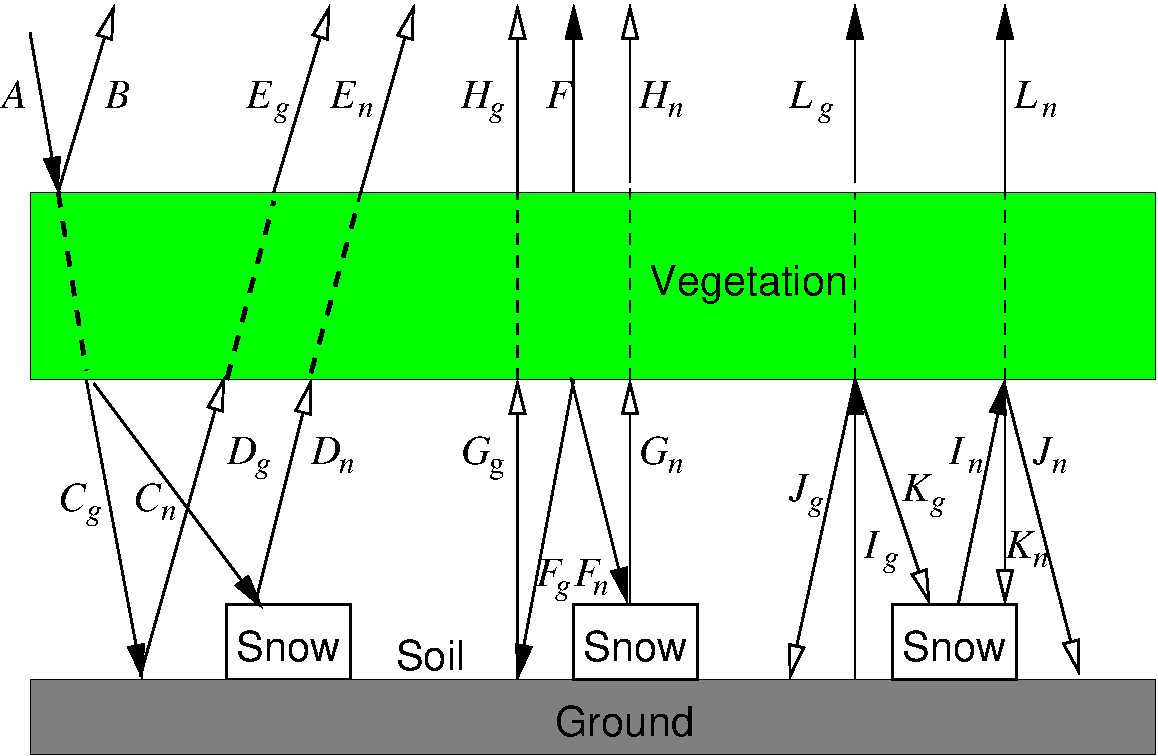
\includegraphics[angle=0, width=12cm, clip=true, trim=0cm 0cm 0cm 0cm]{\EPSDIR/lwnet_meb.pdf}}
\caption{Simple schematic for longwave radiation transfer for one
reflection and up to three emitting surfaces (in addition to the
down-welling atmospheric flux). Hollow arrows indicate
fluxes after one reflection.}
\label{fig:meb_lwsnow_vg}
\end{figure}
%%%%%%%%%%%%%%%%%%%%%%%%%%%%%%%%%%%%%%



The effective surface radiative temperature (which may be required by the atmospheric radiation
scheme or for comparison with satellite-based data etc.) 
is diagnosed as
%
%%%%%%%%%%%%%%%%%%%%%%%%%
\begin{equation}
  \label{eq:meb_lwup_ts_total_eff}
T_{rad} = {\left[\frac{LW\uparrow - LW\downarrow
      \left(1-{\overline\epsilon}_s\right)}
{{\overline\epsilon}_s \, \sigma}\right]}^{1/4}
%
\end{equation}
%%%%%%%%%%%%%%%%%%%%%%%%%
%
where $\sigma$ is the Stefan-Boltzmann constant, and 
${\overline\epsilon}_s$ represents
the effective surface emissivity. In Eq.~\ref{eq:meb_lwup_ts_total_eff},
there are two knowns ($LW$ fluxes) and two unknowns ($T_{rad}$ and
${\overline\epsilon}_s$). Here we opt to pre-define
${\overline\epsilon}_s$ in a manner which is consistent with the
various surface contributions as
%
%%%%%%%%%%%%%%%%%%%%%%%%%
\begin{equation}
  \label{eq:meb_emis_sfc_eff}
{\overline\epsilon}_s = p_{sng}\,{\overline\epsilon}_{sn} + \left( 1 - p_{sng}\right){\overline\epsilon}_{sg}
%
\end{equation}
%%%%%%%%%%%%%%%%%%%%%%%%%
%
The canopy-absorption weighted 
effective snow and ground emissivities are defined, respecitvely, as
%
%%%%%%%%%%%%%%%%%%%%%%%%%
%\begin{subequations}
\begin{align}
 \label{eq:meb_lw_emis_sfc_terms_n}
{\overline\epsilon}_{sn} = & 
        {\overline\sigma}_{n\,LW}       \,\epsilon_v \,+\, 
\left(1-{\overline\sigma}_{n\,LW}\right)\,\epsilon_n
\\
 \label{eq:meb_lw_emis_sfc_terms_g}
{\overline\epsilon}_{sg} = & 
        {\overline\sigma}_{g\,LW}       \,\epsilon_v \,+\, 
\left(1-{\overline\sigma}_{g\,LW}\right)\,\epsilon_g
%
\end{align}
%\end{subequations}
%%%%%%%%%%%%%%%%%%%%%%%%%
%
where $\epsilon_v$, $\epsilon_g$ and $\epsilon_n$ represent 
the emissivities of the vegetation, snow-free ground and 
the ground-based snowpack, respectively. 
The ground and vegetation emissivities are given by ECOCLIMAP for
spatially distributed simulations, or they can be prescribed for local
scale studies. The snow emissivity is currently defined as $\epsilon_n=0.99$.
%based on the flood-weighted water and soil
%emissivities as
%
%%%%%%%%%%%%%%%%%%%%%%%%%
%\begin{equation}
%  \label{eq:meb_lwup_emis_flood}
%{\overline\epsilon}_g = p_{ff} \epsilon_{ff} + \left(1-p_{ff}\right)\epsilon_g
%
%\end{equation}
%%%%%%%%%%%%%%%%%%%%%%%%%
%
%where $\epsilon_{ff}$ is the emissivity of the flooded area,
%and $\epsilon_g$ is the snow-free flood-free ground emissivity.
%
The effect of longwave absorption through the non-snow buried
part of the vegetation canopy is included as
%
%%%%%%%%%%%%%%%%%%%%%%%%%
%\begin{subequations}
\begin{align}
 \label{eq:meb_lw_sig_emis_sfc_terms_n}
{\overline\sigma}_{n\,LW} = & 
\left[1 \,-\, p_{sng} \,-\, p_{n\alpha}\left(1-p_{sng}\right)\right]
\sigma_{LW} 
\,+\, 
\left[p_{sng} \,+\, p_{n\alpha}\left(1-p_{sng}\right)\right]
\sigma_{f\,LW}
\\
 \label{eq:meb_lw_sig_emis_sfc_terms_g}
{\overline\sigma}_{g\,LW} = & 
\left[1 \,-\, p_{sng}\left(1-p_{n\alpha}\right)\right]
\sigma_{LW} 
\,+\, 
p_{sng}\left(1-p_{n\alpha}\right)
\sigma_{f\,LW}
%
\end{align}
%\end{subequations}
%%%%%%%%%%%%%%%%%%%%%%%%%
%
where the canopy absorption is defined as
%
%%%%%%%%%%%%%%%%
\begin{equation}
\label{eq:meb_sigma_lw}
%
\sigma_{LW} = 1 - {\mathrm{exp}}\left( -\tau_{LW} \, LAI \right) = 1 - \chi_v
%
\end{equation}
%%%%%%%%%%%%%%%%
%
and $\tau_{LW}$ represents a longwave radiation transmission factor which can be species 
(or land classification) dependent, and $\chi_v$ is defined as a
vegetation view factor. 
%
The absorption over the under-story snow-covered fraction of the grid
box is modeled quite simply from Eq.~\ref{eq:meb_sigma_lw} as
%
%%%%%%%%%%%%%%%%
\begin{equation}
\label{eq:meb_sigma_f_lw}
%
\sigma_{f\,LW} \,=\, 
%1 - {\mathrm{exp}}\left[ -\tau_{LW} \, LAI
% \left(1-p_{n\alpha}\right)\right] \,=\, 
1 - {\mathrm{exp}}\left[ -\tau_{LW} \, LAI_n \right]
%
\end{equation}
%%%%%%%%%%%%%%%%
%
so that transmission is unity (no absorption or reflection by the canopy: 
${\overline\sigma}_{LW}=\sigma_{f\,LW}=0$) when $p_{n\alpha}=1$
(i.e. when the canopy has been buried by snow).
%When none of the canopy is buried by the main snowpack then $p_{n\alpha}=0$ so
%that $p_{sng}^\prime=p_{sng}$ which means that
%${\overline\sigma}_{LW}=\sigma_{f\,LW}=\sigma_{LW}$.
$LAI_n$ is used to represent the $LAI$ which has been reduced owing to
burial by the snowpack and is simply defined as:
%
%%%%%%%%%%%%%%%%%%%%%%%%%
\begin{equation}
  \label{eq:meb_lai_snow_modif}
LAI_n = LAI \left(1 \,-\, p_{n\,\alpha}\right)
\end{equation}
%%%%%%%%%%%%%%%%%%%%%%%%%
%
From Eq.s~\ref{eq:meb_emis_sfc_eff}-\ref{eq:meb_lw_sig_emis_sfc_terms_g}, it
can be seen that when there is no snowpack (i.e. $p_{sng}=0$ and
$p_{n\alpha}=0$),
%or flooded fraction ($p_{ff}=0$),
then the effective surface emissivity is simply an absorption-weighted
soil-vegetation value defined as ${\overline\epsilon}_s =  
\sigma_{LW}       \,\epsilon_v \,+\, 
\left(1-\sigma_{LW}\right)\,\epsilon_g$.
%
%See Appendix~\ref{app:meb_lwrad_flux_expressions} for the derivation of
%the net longwave radiation terms in Eq.~\ref{eq:meb_lwup_resid}.


%%%%%%%%%%%%%%%%%%%%%%%%%%%%%%%%%%%%%%%%%%%%%%%%%%%%%%%%%%%%%%%%%%%%%%%%%%%%%%%%%%

%The flooded fraction of the gridbox uses a ground-flooded zone composite
%energy budget, so to consider water surfaces we have defined
%an effective snow-free ground albedo as
%%
%%%%%%%%%%%%%%%%%%%%%%%%%%
%\begin{equation}
%  \label{eq:swup_resid_flood}
%{\overline\alpha}_g = p_{ff} \alpha_{ff} + \left(1-p_{ff}\right)\alpha_g
%%
%\end{equation}
%%%%%%%%%%%%%%%%%%%%%%%%%
%
%where $p_{ff}$ is the sub-grid flooded fraction, $\alpha_{ff}$ is the effective albedo of the flooded area,


The complete expression for the vegetation canopy net longwave radiation 
with an infinite number of reflections can be expressed as a
series expansion 
(e.g. Braud, 2000\nocite{braud_00}) 
as a function of the
temperatures of the emitting surfaces ($T_v$, $T_{g,1}$, 
$T_{n,1}$), their respective emissivities
($\epsilon_v$, $\epsilon_g$ and $\epsilon_n$) and the canopy longwave
absorption function,
$\sigma_{LW}$ (Eq.~\ref{eq:meb_sigma_lw}).
%
The MEB expressions are derived by explicitly expanding
the series 
%This is done to facillitate computing the flux components
%for the different surfaces explicitly (we compare our approximate expressions to
%the series approximations in the next section).
%
%First
and assuming one reflection from each emitting source, which is
a good approximation since emissivities are generally close to unity
(fluxes from a single reflection are proportional to $1-\epsilon_x$ where $x$ represents
$g$, $v$ or $n$, and $\epsilon$ is close
to unity for most natural surfaces).
%Therefore all higher order terms which involve products of reflected fluxes
%are neglected (since such terms will be at least an order of magnitude
%smaller than the terms involing a single reflection).

Snow is considered to be intercepted by the vegetation canopy and to accumulate
on the ground below. 
%The corresponding schematic of the radiative transfer is shown in
%Fig.~\ref{fig:lwsnow_vg}.
%
The canopy-intercepted snow is treated using a composite approach,
so that the canopy temperature, $T_v$, represents the effective temperature of
the canopy-intercepted snow composite. The canopy emissivity is therefore simply defined as
%
%%%%%%%%%%%%%%%%
\begin{equation}
\label{eq:meb_emis_v_n}
%
{\overline\epsilon}_v = \left( 1 - p_{nv}\right) \epsilon_v \,+\, p_{nv}\,\epsilon_{n}
%
\end{equation}
%%%%%%%%%%%%%%%%
%
%where 
%$p_{nv}$ represents the fraction of the canopy covered by intercepted snow, and
%$\epsilon_{n}$ represents the emissivity of the intercepted snow.
%
In order to facilitate the use of a distinct multi-layer snow process
scheme, we
split the fluxes between those interacting with the snowpack and the
snow-free ground.
%
The expressions for the snow-free 
%understory layer 
surface 
are
%
%%%%%%%%%%%%%%%%%%%%%%%%%
\begin{subequations}\label{eq:meb_lw_g_n_terms}
\begin{align}
 \label{eq:meb_lw_g_n_terms_a}
A_{g} = & LW\downarrow \,\left(1-p_{sng}\right)
\\
 \label{eq:meb_lw_g_n_terms_b}
B_{g} = & A_{g}\,\sigma_{LW}\,\left(1-{\overline\epsilon}_v\right)
\\
 \label{eq:meb_lw_g_n_terms_c}
C_{g} = & A_{g}\,\left(1-\sigma_{LW}\right)
\\
 \label{eq:meb_lw_g_n_terms_d}
D_{g} = & C_{g} \,\left(1-\epsilon_g\right)
\\
 \label{eq:meb_lw_g_n_terms_e}
E_{g} = & D_{g}\left(1-\sigma_{LW}^\prime\right)
\\
 \label{eq:meb_lw_g_n_terms_f}
F_{g} = & \sigma_{LW}^\prime\, \sigma \, {\overline\epsilon}_v\, T_v^4\,\left(1-p_{sng}\right)
\\
 \label{eq:meb_lw_g_n_terms_g}
G_{g} = & F_{g}\,\left(1-\epsilon_g\right)
\\
 \label{eq:meb_lw_g_n_terms_h}
H_{g} = & G_{g}\,\left(1-\sigma_{LW}^\prime\right)
\\
 \label{eq:meb_lw_g_n_terms_i}
I_{g} = & \sigma \, \epsilon_g\, T_g^4\,\left(1-p_{sng}\right)
\\
 \label{eq:meb_lw_g_n_terms_j}
J_{g} = & I_{g}\,\sigma_{LW}^\prime\,\left(1-{\overline\epsilon}_v\right) \,\left(1-p_{sng}^\prime\right)
\\
 \label{eq:meb_lw_g_n_terms_k}
K_{g} = & I_{g}\,\sigma_{LW}^\prime\,\left(1-{\overline\epsilon}_v\right) \,p_{sng}^\prime
\\
 \label{eq:meb_lw_g_n_terms_l}
L_{g} = & I_{g}\,\left(1-\sigma_{LW}^\prime\right)
%
\\
 \label{eq:meb_lw_g_n_terms_png}
p_{sng}^\prime = & p_{sng}\left(1-p_{n\alpha}\right)
%
\end{align}
\end{subequations}
%%%%%%%%%%%%%%%%%%%%%%%%%
%
and the equations for the snow-covered under-story fraction are
%
%%%%%%%%%%%%%%%%%%%%%%%%%
\begin{subequations}\label{eq:meb_lw_n_n_terms}
\begin{align}
 \label{eq:meb_lw_n_n_terms_a}
A_{n} = & LW\downarrow \,p_{sng}
\\
 \label{eq:meb_lw_n_n_terms_b}
B_{n} = & A_{n}\,\sigma_{f\,LW}\,\left(1-\epsilon_v\right)
\\
 \label{eq:meb_lw_n_n_terms_c}
C_{n} = & A_{n}\,\left(1-\sigma_{f\,LW}\right)
\\
 \label{eq:meb_lw_n_n_terms_d}
D_{n} = & C_{n} \,\left(1-\epsilon_n\right)
\\
 \label{eq:meb_lw_n_n_terms_e}
E_{n} = & D_{n}\left(1-\sigma_{LW}^\prime\right)
\\
 \label{eq:meb_lw_n_n_terms_f}
F_{n} = & {\overline\sigma}_{f\,LW}\, \sigma \, \epsilon_v\, T_v^4\,p_{sng}
\\
 \label{eq:meb_lw_n_n_terms_g}
G_{n} = & F_{n}\,\left(1-\epsilon_n\right)
\\
 \label{eq:meb_lw_n_n_terms_h}
H_{n} = & G_{n}\,\left(1-\sigma_{LW}^\prime\right)
\\
 \label{eq:meb_lw_n_n_terms_i}
I_{n} = & \sigma \, \epsilon_n\, T_n^4\,p_{sng}
\\
 \label{eq:meb_lw_n_n_terms_j}
J_{n} = & I_{n}\,\sigma_{LW}^\prime\,\left(1-\epsilon_v\right) \,\left(1-p_{sng}^{\prime\prime}\right)
\\
 \label{eq:meb_lw_n_n_terms_k}
K_{n} = & I_{n}\,\sigma_{LW}^\prime\,\left(1-\epsilon_v\right) \, p_{sng}^{\prime\prime}
\\
 \label{eq:meb_lw_n_n_terms_l}
L_{n} = & I_{n}\,\left(1-\sigma_{LW}^\prime\right)
%
\\
 \label{eq:meb_lw_n_n_terms_png}
p_{sng}^{\prime\prime} = & p_{sng} \,+\, p_{n\alpha}\left(1-p_{sng}\right)
%
\end{align}
\end{subequations}
%%%%%%%%%%%%%%%%%%%%%%%%%
%
where the different terms are again
indicated in Fig.~\ref{fig:meb_lwsnow_vg}.
%
In MEB, the ground-based snowpack depth can increase to the point that
it buries the canopy, thus
for both the snow-covered and snow free under-story fractions 
a modified snow fraction is defined as
%
%%%%%%%%%%%%%%%%
\begin{equation}
\label{eq:meb_sigma_lw_avg}
%
\sigma_{LW}^\prime = \left(1-p_{sng}^\prime\right)\sigma_{LW} \,+\,
p_{sng}^\prime \,\sigma_{f\,LW}
%
\end{equation}
%%%%%%%%%%%%%%%%
%
The factor, $\sigma_{f\,LW}$, over the understory snow-covered fraction of the grid
box is modeled quite simply from Eq.~\ref{eq:meb_sigma_f_lw}.
%
%%%%%%%%%%%%%%%%%
%\begin{equation}
%\label{eq:meb_sigma_f_lw}
%%
%\sigma_{f\,LW} = 1 - {\mathrm exp}\left[ -\tau_{LW} \, LAI \left(1-p_{n\alpha}\right)\right]
%%
%\end{equation}
%%%%%%%%%%%%%%%%%
%%
%so that transmission is unity (no absorbtion or reflection by the canopy: 
%$\sigma_{LW}^\prime=\sigma_{f\,LW}=0$) when $p_{n\alpha}=1$
%(i.e. when the canopy has been buried by snow).
%When none of the canopy is buried by the main snowpack then $p_{n\alpha}=0$ so
%that $p_{sng}^\prime=p_{sng}$ which means that $\sigma_{LW}^\prime=\sigma_{f\,LW}=\sigma_{LW}$.
%
%
The inclusion of the snow-buried canopy fraction in
Eq.s~\ref{eq:meb_lw_g_n_terms_png} and \ref{eq:meb_lw_n_n_terms_png}
causes all of the vegetation transmission and below canopy fluxes to vanish as
$p_{sng}$ and $p_{n\alpha}\rightarrow 0$ so that the only longwave
radiative exchanges occur between the atmosphere and the snowpack in
this limit. 




%=========================================================================================================
\subsubsection{Heat Conduction fluxes}
\label{sec:meb_energy_budget_cond}
%=========================================================================================================

%The sub-surface snow and ground heat conduction fluxes are modeled 
%using Fourier's Law ($G=\lambda\partial T/\partial z$). 
The heat
conduction fluxes in Eq.s~\ref{eq:meb_cgdtgdt_three}-\ref{eq:meb_cndtndt_three}
are modeled 
using Fourier's Law ($G=\lambda\partial T/\partial z$)
and have been defined in previous sections (since MEB uses
either the multilayer diffusive or 2 to 3 layer Force-Restore 
hydrology/soil configurations, coupled to the explicit multilayer snow
scheme ES).
%
The main potential difference between ISBA and ISBA-MEB is that
the heat capacity and thermal conductivity for the ground 
depend either on the thermal properties of the soil
(possibly including organic content)
or on the thermal
properties of the forest litter
in the uppermost layer (Napoly et al., 2017)\nocite{napoly_ea_2017}: 
this parameterization
is described in more detail in Section~\ref{sec:meb_litter}.
%The snow thermal property parameterization is described in \citet{Decharme16}.

%=========================================================================================================
\subsubsection{Aerodynamic Resistances}
\label{sec:meb_resistances} 
%=========================================================================================================

The resistances between the surface and the overlying atmosphere, $R_{a\,n-a}$
and $R_{a\,c-a}$, are based on the values of $C_H$ 
computed from Eq.~\ref{eq:isba_heat_transfer_coef}
between
the overyling atmosphere and the snow surface, and between
the overyling atmosphere and the canopy air space, respectively, where
$C_{Hx}={\left(V_a R_{a\,x-a}\right)}^{-1}$.

%\citet{louis_79}
%modified by \citet{mascart_ea_95} to account for different roughness 
%length values for heat and momentum as in ISBA.
%: the full expressions are given 
%in \citet{noilhan_mahfouf_96}.

%\subsubsection{Aerodynamic Resistance between the bulk vegetation
%layer and the canopy air}

The aerodynamic resistance between the vegetation canopy and the
surrounding airspace can be defined as
%
%%%%%%%%%%%%%%%%%%%%%%%%%
\begin{equation}
  \label{eq:meb_bulk_canopy_resis}
  R_{a\,vg-c} = {\left( g_{av} \,+\, g_{av}^\ast \right)}^{-1}
\end{equation}
%%%%%%%%%%%%%%%%%%%%%%%%%
%
The parameterization of the bulk canopy aerodynamic conductance, $g_{av}$, 
between the canopy and the canopy air is based on 
Choudhury and Monteith (1988)\nocite{Choudhury88}.
It is defined as
%
%%%%%%%%%%%%%%%%%%%%%%%%%
\begin{equation}
  \label{eq:meb_condrb}
  g_{av} = 
%{\Bigg\lbrace
\frac{2 \, LAI \, a_{av}}{\phi_v^\prime}\left(\frac{u_{hv}}{lw}\right)^{1/2}[1-\exp(-\phi_v^\prime/2)].
%\Bigg\rbrace}^{-1}
\end{equation}
%%%%%%%%%%%%%%%%%%%%%%%%%
%
where 
%the resistance in Eq.~\ref{eq:meb_bulk_canopy_resis} is simply
%$R_{av}=g_{av}^{-1}$.
$u_{hv}$ represents the wind speed at the top of the canopy
(m s$^{-1}$),
$LAI$ is the leaf area index (m$^{2}$ m$^{-2}$), and the remaining parameters are
defined in Table~\ref{independent}.
%
The conductance accounting for the free convection correction
from Sellers et al. (1986)\nocite{Sellers86}
is expressed as
%
%%%%%%%%%%%%%%%%%%%%%%%%%
\begin{equation}
  \label{eq:meb_freeconv}
  g_{av}^\ast = \left[ \frac{LAI}{890} \left(\frac{T_{v} -
        T_{c}}{lw}\right)^{1/4}\right]
\hskip1.in \left( T_{v} \geq T_{c} \right)
\end{equation}
%%%%%%%%%%%%%%%%%%%%%%%%%
%
Note that this correction is only used for unstable conditions.
%
The effect of snow burying the vegetation impacts the aerodynamic
resistance of the canopy is simply modeled by modifying the $LAI$
to obtain $LAI_n$ using Eq.~\ref{eq:meb_lai_snow_modif}.
%
The $LAI_n$ is used in
Eq.~\ref{eq:meb_bulk_canopy_resis} to compute $R_{a\,vn-c}$, and this
resistance is limited to 5000 s m$^{-1}$ as $LAI_n \rightarrow 0$.


%\subsubsection{Aerodynamic Resistance between the ground and the canopy air}

%%%%%%%%%%%%%%%%%%%%%%%%%%%%%%%%%%%%%%%%%%%%%%%%%%%%%%%%%%%%%%%%%%%%%%%%%%%%%

The resistance between the ground and the canopy air space is defined as
%
%%%%%%%%%%%%%%%%%%%%%%%%%
\begin{equation}
  \label{eq:meb_resistance_stabcor}
R_{ag-c} = R_{ag\,n}/\psi_H
%
\end{equation}
%%%%%%%%%%%%%%%%%%%%%%%%%
%
where $R_{ag\,n}$ is the default resistance value for neutral conditions. 
%(from Eq.~\ref{eq:meb_rd}).
The stability correction term, $\psi_H$, depends on the canopy
structural parameters, wind speed and temperature gradient
between the surface and the canopy air.
%
The aerodynamic resistance is also based on
Choudhury and Monteith (1988)\nocite{Choudhury88}.
It is assumed that the eddy diffusivity, $K$ (m$^2$ s$^{-1}$), 
in the vegetation layer
follows an exponential profile:
%
%%%%%%%%%%%%%%%%%%%%%%%%%
\begin{equation}
  \label{eq:meb_k_prof}
K\left(z\right) = K\left(z_{hv}\right) \,
\exp\left[\phi_v \left(1-{\frac{z}{z_{hv}}}\right)\right] 
\end{equation}
%%%%%%%%%%%%%%%%%%%%%%%%%
%
where $z_{hv}$ represents the canopy height.
Integrating the reciprocal of the diffusivity defined
in Eq.~\ref{eq:meb_k_prof} from $z_{0g}$ to $d + z_{0v}$ yields
%
%%%%%%%%%%%%%%%%%%%%%%%%%
\begin{equation}
  \label{eq:meb_rd}
  R_{ag\,n} = \frac{z_{hv}}{\phi_v \, K\left(z_{hv}\right)}
\Bigg\lbrace
\exp\left[\phi_v \left(1-{\frac{z_{0g}}{z_{hv}}}\right)\right] \,-\, 
\exp\left[\phi_v \left(1-{\frac{d +
             z_{0v}}{z_{hv}}} \right)\right] 
\Bigg\rbrace
\end{equation}
%%%%%%%%%%%%%%%%%%%%%%%%%
%
The diffusivity at the canopy top is defined as
%
%%%%%%%%%%%%%%%%%%%%%%%%%
\begin{equation}
  \label{eq:meb_Kh}
  K\left(z_{hv}\right) = k \, u_{\ast hv} \, \left(z_{hv} - d\right) 
%= 
%{\frac{k^2 \, u_{hv} \, \left(z_{hv} - d\right)} 
%{{\mathrm{ln}} \left[ \left(z_{hv} - d\right)/z_{0v}\right] }}
\end{equation}
%%%%%%%%%%%%%%%%%%%%%%%%%
%
The von Karman constant, $k$, has a value of 0.4.
The displacement height is defined as 
(Choudhury and Monteith, 1988)\nocite{Choudhury88}
%
%%%%%%%%%%%%%%%%%%%%%%%%%
\begin{equation}
  \label{eq:meb_disph}
  d = 1.1 \, z_{hv} \, {\mathrm{ln}}\left[1 + {\left(c_d \, LAI_f\right)}^{1/4}\right]
\end{equation}
%%%%%%%%%%%%%%%%%%%%%%%%%
%
where
the leaf drag coefficient, $c_d$, is defined from 
Sellers et al. (1996)\nocite{Sellers96}:
%
%%%%%%%%%%%%%%%%%%%%%%%%%
\begin{equation}
  \label{eq:meb_cd}
  c_d = 1.328 \, \left[\frac{2}{{R_e}^{1/2}}\right] + 
0.45 \left[ \frac{1}{\pi}(1-\chi_L) \right]^{1.6}
\end{equation}
%%%%%%%%%%%%%%%%%%%%%%%%%
%
$\chi_L$ represents the Ross-Goudriaan leaf angle distribution function, which has
been estimated according to 
Monteith (1975)\nocite{Monteith75}
(see Table~\ref{meb_independent}), and
$R_e$ is the Reynolds number defined as
%
%%%%%%%%%%%%%%%%%%%%%%%%%
\begin{equation}
  \label{eq:meb_Re}
  {R_e} = \frac{u_l \, lw}{\upsilon}.
\end{equation}
%%%%%%%%%%%%%%%%%%%%%%%%%
%
%The unstable transfer correction for $r_{ag}=r_{ag}/\psi_H$ according to \cite{Sellers86},
%where
%
%%%%%%%%%%%%%%%%%%%%%%%%%
%\begin{equation}
%  \label{eq:meb_phih}
%  \psi_H = \left[ 1 + 9 \frac{T_{g} - T_{c}}{T_{g} u_{hv}^2} z_{hv} \right]^{1/2}.
%\end{equation}
%%%%%%%%%%%%%%%%%%%%%%%%%
%

The friction velocity at the top of the vegetation canopy is
defined as
%
%%%%%%%%%%%%%%%%%%%%%%%%%
\begin{equation}
  \label{eq:meb_ustar_cantop}
u_{\ast hv} = {\frac{k \, u_{hv}}
{{\mathrm{ln}}\left[
\left( z_{hv} - d \right)/z_{0v}\right]}}
\end{equation}
%%%%%%%%%%%%%%%%%%%%%%%%%
%
where the wind speed at the top of the canopy is
%
%%%%%%%%%%%%%%%%%%%%%%%%%
\begin{equation}
  \label{eq:meb_u_cantop}
u_{hv} = f_{hv} \, V_a
\end{equation}
%%%%%%%%%%%%%%%%%%%%%%%%%
%
and $V_a$ represents the wind speed at the reference height, $z_a$,
above the canopy. 
%
The canopy height is defined based on vegetation
class and climate within ECOCLIMAP as a primary parameter. It can
also be defined using an external dataset, such as from a satellite-derived product (as a function of space and time). The vegetation
roughness length for momentum is then computed as a secondary
parameter as a function of the vegetation canopy height.
%
The factor $f_{hv}$ ($\leq 1$) is a stability dependent adjustment factor
%(see Appendix~\ref{app:f_stab_factor}).
%The expressions for the stability factor $f_{hv}$ (Eq.~\ref{eq:u_cantop}) which is used 
%to compute the wind at the top of the vegetation canopy, $u_{hv}$, are 
taken from the RCA LSM 
(Samuelsson et al., 2006; Samuelsson et al., 2011)\nocite{Samuelsson06,Samuelsson11}.
They are defined as
%
%%%%%%%%%%%%%%%%%%%%%%%%%%%%%%
\[ f_{hv} = \left\{ \begin{array}{ll}
        \left( C_{v,N} \,+\, C_{v,S}\right) \sqrt{C_D} \, /k
& \mbox{if $R_i > 0 $}
\\
        \left( C_{v,N} \,+\, C_{v,U}\right) \sqrt{C_D} \, /k
& \mbox{if $R_i \leq 0$}
\end{array} 
\right. \] 
%%%%%%%%%%%%%%%%%%%%%%%%%%%%%%
%%%%%%%%%%%%%%%%%%%%%%%%%
%\begin{subequations}
%\begin{align}
%
%\label{eq:meb_fv_velc_stable} 
%f_{hv} =& \left( C_{v,N} \,+\, C_{v,S}\right) \sqrt{C_D} \, /k
%\hskip.5in
%\left(R_i > 0 \right)
%\\
%%
%\label{eq:meb_fv_velc_unstable} 
%    =& \left( C_{v,N} \,+\, C_{v,U}\right) \sqrt{C_D} \, /k
%\hskip.5in
%\left(R_i \leq 0 \right)
%%
%\end{align}
%\end{subequations}
%%%%%%%%%%%%%%%%%%%%%%%%%
%
where the Richardson number, $R_i$, is defined 
in Eq.~\ref{eq:meb_canopy_ground_rich}.
The coefficients are defined as
%
%%%%%%%%%%%%%%%%%%%%%%%%%
\begin{align}
%
\label{eq:meb_fv_velc_neutral_c} 
C_{v,N} =& {\mathrm{ln}} \Bigg\lbrace 
1 \,+\, \phi_z
\left[\exp \left({\frac{k}{\sqrt{C_{DN}}}}\right) - 1\right]
\Bigg\rbrace 
\\
%
\label{eq:meb_fv_velc_stable_c} 
C_{v,S} =& -
\phi_z
\left(
{\frac{k}{\sqrt{C_{DN}}}}-{\frac{k}{\sqrt{C_{D}}}}
\right)
\\
%
\label{eq:meb_fv_velc_unstable_c} 
C_{v,U} =& -{\mathrm{ln}} \Bigg\lbrace 
1 \,+\, \phi_z
\left[\exp \left(
{\frac{k}{\sqrt{C_{DN}}}}-{\frac{k}{\sqrt{C_{D}}}}
\right) 
- 1\right]
\Bigg\rbrace 
%
\end{align}
%%%%%%%%%%%%%%%%%%%%%%%%%
%
where the drag coefficient, $C_D$, and the drag coefficient for
neutral conditions, $C_{DN}$, are computed between the
canopy air space 
%(at height $z_c$)
and the free atmosphere above using the standard ISBA
surface layer
transfer functions (Eq.~\ref{eq:isba_drag_transfer_coef} and
Eq.~\ref{eq:isba_drag_transfer_coef_neutral}, respectively).
%\citep{noilhan_mahfouf_96}.




The dimensionless height scaling factor
is defined as 
%
%%%%%%%%%%%%%%%%%%%%%%%%%
\begin{equation}
%
\label{eq:meb_z_ratio_measure} 
\phi_z = {\frac{\left(z_{hv}-d\right)}{z_r}}
\hskip1.in
\left( \phi_z\leq 1 \right)
\end{equation}
%%%%%%%%%%%%%%%%%%%%%%%%%
%
The reference height is defined as $z_r=z_a-d$
for simulations where the reference height is sufficiently above
the top of the vegetation canopy. This is usually the case for local
scale studies using observation data.
When MEB is coupled to an atmospheric model, however, the lowest model
level can be below the canopy height, so for coupled model
simulations
$z_r = {\mathrm{max}}\left(z_a,\,z_{hv}-d+z_{min}\right)$
where $z_{min}=2$ (m).


%\subsubsection{Stability Correction}

Finally, the stability correction 
factor from Eq.~\ref{eq:meb_resistance_stabcor} is defined
as
%
%%%%%%%%%%%%%%%%%%%%%%%%%
\begin{subequations}
\begin{align}
  \label{eq:meb_unstable_cor_rich}
\psi_H & = {\left( 1 \,-\, a_{hv}\,R_i\right)}^{1/2}
\hskip2.3in \left( R_i \leq 0 \right)
\\
%
%\label{eq:meb_stable_cor_rich}
%
%\psi_H & = {\left( 1 \,-\, a_{hv}\,R_i\right)}^{1/2}
%\hskip2.3in \left( R_i \leq 0\right)
%\\
%
%\label{eq:meb_unstable_cor_rich_new}
%\psi_H &= {\left( 1 \,-\, a_{hv}\,R_i\right)}^{1/2} 
%\hskip2.5in \left( R_i \leq 0 \right)
%\\
\label{eq:meb_stable_cor_rich_new_trans}
& = 
%
%OLD%{\left[ 1 \,+\, b\, \left({\frac{R_i}{R_{i,crit}}}\right)\right]}^{-2} \,\,=\,\,
%OLD%{\left( 1 \,+\, b_{hv}\,R_i\right)}^{-2}
%OLD%\hskip.5in \left( R_i > 0 \right)
%
{\frac{1}{1 + b\, R_i {\left(1+c\,R_i\right)}^{1/2}}}
\left[{ 1 \,+\, \left({\frac{R_i}{R_{i,crit}}} \right) \left(f_{z0} - 1 \right)}\right]
\hskip.25in \left( R_i > 0 \,\,{\mathrm{and}}\,\, R_i \leq R_{i,crit} \right)
\\
\label{eq:meb_stable_cor_rich_new}
& = 
%
{\frac{f_{z0}}{1 + b\, R_i {\left(1+c\,R_i\right)}^{1/2}}} 
\hskip2.in \left( R_i > R_{i,crit}\right)
%
\end{align}
\end{subequations}
%%%%%%%%%%%%%%%%%%%%%%%%%
%
where the Richardson number is defined as
%
%%%%%%%%%%%%%%%%%%%%%%%%%
\begin{equation}
  \label{eq:meb_canopy_ground_rich}
R_i = {\frac { -g\,z_{hv}\,\left(T_s - T_c \right)}{T_s \, {u_{hv}}^2}}
%
\end{equation}
%%%%%%%%%%%%%%%%%%%%%%%%%
%
Note that strictly speaking, the temperature factor in the denominator should be defined as
$\left(T_s+T_c\right)/2$, but this has only a minor impact for our
purposes.
%
The so-called critical Richardson number, $R_{i,crit}$, is set to 0.2.
This parameter has been defined assuming that
some turbulent exchange is likely always present (even if intermittent), 
but it is recognized 
that eventually a more robust approach should be developed for very
stable surface layers. 
%(e.g. )\nocite{galperin2007}.
%
The expression for unstable conditions
(Eq.~\ref{eq:meb_unstable_cor_rich}) 
is from 
Sellers et al. (1996)\nocite{Sellers96} 
where
the structural parameter is defined as $a_{hv}=9$. 
%
%Eq.~\ref{eq:meb_unstable_cor_rich} was likely developed with unstable conditions in mind, and it also
%works for slightly stable conditions. But note that one can readily see from
%Eq.~\ref{eq:meb_unstable_cor_rich} that $R_i$ is constrained to be $\leq
%1/{a_{hv}}$, so that a threshold value of either $\phi_H$ or $R_i$ must
%be prescribed for stable conditions.
%a square root of a negative number. 
%So, a somewhat arbitrary threshold must be defined to prevent this.
%In MEB, it was initially decided to define a critical Richardson number as 
%
%%%%%%%%%%%%%%%%%%%%%%%%%%
%\begin{equation}
%  \label{eq:meb_rich_crit_gc}
%R_{ic} = \left[ 1 \, - \, \left({\frac {1}{R_{acf}}}\right) \right]{\frac {1}{a_{hv}}}
%%
%\end{equation}
%%%%%%%%%%%%%%%%%%%%%%%%%%
%
%where the value enclosed in brackets is less than unity. In studies done by C. Canac et al., a 
%value of $R_{acf}=200$ was used, therefore $R_{ic}\approx 0.11$. 
%
%In fact, the stable parameterization becomes quite important
%For the case of snowpack underlying the canopy, very stable
%conditions can develop, especially during spring snow melt, so that the
%model can become quite sensitive to the form of $\phi_H$.
%aabtmptest
%First, simply from a theoretical standpoint, $R_{ic}=0.11$ is significantly larger than the usual limit value of 0.20
%(and for snowpack, such large Richardson numbers can be commonplace).
%Second, small changes
%For example, if Eq.~\ref{eq:meb_unstable_cor_rich} is used for stable
%conditions, 
%relatively small changes 
%in $R_i$ can result in large changes in $\psi_H$, which is counter to what is usually done for stable conditions
%(generally, $\psi_H \rightarrow 0$ gradually/asymptotically as $R_i\rightarrow \infty$). 
%Finally, usually there is a point of inflection
%in the curve describing $\psi_H$ at $R_i=0$, so that there is a exponential-type drop off in turbulent
%exchange for $R_i >0$. If this is not the case, large
%turbulent exchange can occur during snow melt conditions, resulting in
%large negative heat fluxes and excessive melt rates.

%%%%%%%%%%%%%%%%%%%%%%%%%%%%%%%%%%%%%%
\begin{figure}[!b]
\centerline{
%\includegraphics[angle=270, width=11cm, clip=true, trim=0cm 0cm 0cm 0cm]{FIGURES/psi_H_z0-z0h.pdf}}
\includegraphics[angle=270, width=14cm, clip=true, trim=0cm 0cm 0cm 0cm]{\EPSDIR/psi_H_z0-z0h.ps}}
\caption{Stability correction term is shown using the Sellers formulation 
  for $R_i \leq 0$ while the function for stable conditions adapted
  from ISBA ($R_i > 0$) for two ratios of $z_{0g}/z_{0gh}$. The ground surface roughness length is
  defined in Table~\ref{meb_independent}.}
\label{fig:stab_cor_gc}
\end{figure}
%%%%%%%%%%%%%%%%%%%%%%%%%%%%%%%%%%%%%%

%\subsection{New stable formulation}
%
It is generally accepted 
that there is a need to improve the parameterization of the exchange
coefficient for
extremely stable conditions typically encountered over snow
(e.g.s Niu and Yang, 2004; Andreadis et al., 2009)
\nocite{niu_yang_2004,andreadis_ea_2009}.
%
Since the goal here is not to develop a new parameterization,
we simply modify the expression for stable conditions
by using the standard function from ISBA. 
The standard ISBA stability correction for stable conditions is given
by Eq.~\ref{eq:meb_stable_cor_rich_new}
where $b=15$ and $c=5$.
%\citep{noilhan_mahfouf_96}.
The factor which takes into account differing roughness lengths for heat and momentum
is defined as
%
%%%%%%%%%%%%%%%%%%%%%%%%%
\begin{equation}
  \label{eq:meb_stable_cor_rich_orig_isba}
f_{z0} = 
%\left[{ 
{\frac{ {\mathrm{ln}}\left(z_{hv}/z_{0g}   \right) }
      { {\mathrm{ln}}\left(z_{hv}/z_{0gh}\right) } }
%}\right]
%
\end{equation}
%%%%%%%%%%%%%%%%%%%%%%%%%
%
where $z_{0gh}$ is the ground roughness length for scalars.
%, and the reference height, $z$, is set to $z_{hv}$.
The weighting function (i.e. ratio of $R_i$ to $R_{i,crit}$) in Eq.~\ref{eq:meb_stable_cor_rich_new_trans} 
is used in order to avoid a discontinuity at $R_i=0$ (the roughness length factor effect vanishes at $R_i=0$)
in Eq.~\ref{eq:meb_stable_cor_rich_new}.
%Eq.~\ref{eq:meb_stable_cor_rich_new} is identical to that
%proposed 
%by \citet{noilhan_mahfouf_96} for stable conditions.
%
%
An example of Eq.~\ref{eq:meb_stable_cor_rich_new} 
is shown in Fig.~\ref{fig:stab_cor_gc} using the $z_{0g}$ from
Table~\ref{independent}, 
%vegetation heights, $z_{hv}$, of 5 and 10 m,
and for $z_{0gh}/z_{0g}$ of 0.1 and 1.0.
%
Finally, the resistance between the ground-based snowpack, $R_{a\,n-c}$, and the canopy air
use the same expressions as for the aerodynamic resistance between the
ground and the canopy air outlined herein, but with the surface
properties of the snowpack (namely the roughness length and snow surface temperature).
%Note that as the vegetation becomes buried (i.e. $p_{n\,alpha}>0$), 


%%%%%%%%%%%%%%%%%%%%%%%%%%%%%%
\begin{table}[h]
\caption{Surface vegetation canopy turbulence parameters which are constant.}
\begin{center}
\begin{footnotesize}
\begin{tabular}{clllll}
\hline
Symbol		& Definition			& Unit		& Value	& Reference		& Comment \\
\hline
\hline
%$g$		& Acceleration of gravity	& m s$^{-2}$	& 9.81	\\
%$G_2$		& Adjustment factor		& -		& 0.75	& \nocite{Xue91}	& Eq. 13 \\
%$k$		& von Karman constant		& -		& 0.4 \\
$a_{av}$		& canopy conductance scale factor & m
s$^{-1/2}$	& 0.01	& 
Choudhury and Monteith (1988)\nocite{Choudhury88}	& Eq. 26 \\
$\phi_v^\prime$	& attenuation coeff. for wind	& -		& 3
& 
Choudhury and Monteith (1988)\nocite{Choudhury88} & p 386 \\
$lw$		& leaf width			& m		& 0.02	\\
$\phi_v$	& attenuation coeff. for mom.	& -		& 2
& 
Choudhury and Monteith (1988)\nocite{Choudhury88} & p 386 \\
$z_{0g}$		& roughness of soil surface	& m		& 0.007	\\
$\chi_L$	& Ross-Goudriaan leaf angle dist. & -		& 0.12
& 
Monteith (1975)\nocite{Monteith75}	& p 26 \\
$u_l$		& Typical local wind speed	& m s$^{-1}$	& 1
& Sellers et al. (1996)\nocite {Sellers96}	& Eq. B7 \\
$\upsilon$	& Kinematic viscos. of air	& m$^2$ s$^{-1}$ & $0.15\times10^{-4}$ \\

\hline
\end{tabular}
\end{footnotesize}
\end{center}
\label{meb_independent}
\end{table}
%%%%%%%%%%%%%%%%%%%%%%%%%%%%%%%%%%%%




%=========================================================================================================
\subsubsection{Ground resistance}
%=========================================================================================================

The soil resistance term is
defined based on 
Sellers et al. (1992)\nocite{sellers_ea_1992} 
as
%
%%%%%%%%%%%%%%%%%%%%%%%%%%
\begin{equation}
\label{eq:meb_resis_grnd}
R_g = {\mathrm{exp}}\left[a_{Rg} - b_{Rg} \,
\left({\overline w_g}/{\overline w_{sat}}\right)\right] \,\,\,.
%
\end{equation}
%%%%%%%%%%%%%%%%%%%%%%%%%%
%
The coefficients are $a_{Rg}=8.206$ and $b_{Rg}=4.255$, and the
vertically averaged volumetric water content and saturated volumetric water content 
are given by ${\overline w_g}$ and ${\overline w_{sat}}$,
respectively. The averaging is done from one to several upper layers.
%
Indeed, the inclusion of an explicit ground surface energy budget
makes it more conceptually straightforward to include a ground
resistance compared to the original composite soil-vegetation
surface.
%, and many models use such a resistance term together with the
%humidity function as it has been shown to both generally improve
%results and it has numerical advantages compared to using the
%so-called alpha parameterization alone 
%
The ground resistance is often used as a surrogate for an additional
resistance arising due to a forest litter layer, therefore
the soil resistance is set to zero 
when the litter layer option is activated. 
Finally, the coefficients $a_{Rg}$ and $b_{Rg}$ were determined from a case study for a
specific location, and could possibly be location dependent. But
currently these values are used, in part, since the
litter formulation is the default
configuration for MEB for forests as it generally gives better surface
fluxes 
(Napoly et al., 2017)\nocite{napoly_ea_2017}.


%----------------------------------------------------------------------------------------



%----------------------------------------------------------------------------------------




%=========================================================================================================
\subsubsection{Water Budget}
\label{sec:meb_water_budget}
%=========================================================================================================

The governing equations for (water) mass for the bulk canopy, and
surface snow and ground layers are written as
%
%%%%%%%%%%%%%%%%%%%%%%%%%
\begin{align}
%
\label{eq:meb_dwrvdt}
{\frac {\partial W_{r}}{\partial t}} = & 
 P_{rv} \,+\, {\mathrm{max}}\left(0, \, -E_{tr}\right) 
- E_{r} \,-\, D_{rv} \,-\, \Phi_{v}
\\
%
\label{eq:meb_dtwrnvdt}
{\frac {\partial W_{r\,n}}{\partial t}} = & 
I_{n} \,-\, U_{n} \,-\, E_{rn} \,+\, \Phi_{v}
%\,+\,  E_{n,v cor} &
%
\\
%
\label{eq:meb_dtwndt}
%p_{sng} \, {\frac {\partial W_{n,1}}{\partial t}} = & P_s \,-\, 
%I_{n} \,+\, U_{n} + 
%\nonumber\\
%& p_{sng} \, \left(
%P_r \,-\, P_{rv} \,+\, D_{rv}
%- F_{nl,1} - E_n
%- \Phi_{n,1}
%+ \xi_{nl,1} 
%\right)
%\\
%
p_{sng} \, {\frac {\partial W_{n,1}}{\partial t}} = & P_s \,-\, 
I_{n} \,+\, U_{n} + 
p_{sng} \, \left(
P_r \,-\, P_{rv} \,+\, D_{rv}
- F_{nl,1} - E_n
+ \Phi_{n,1}
+ \xi_{nl,1} 
\right)
\\
%
\label{eq:meb_dtwgdt} 
\rho_w \, \Delta z_{g,1} {\frac {\partial w_{g,1}}{\partial t}} = & 
\left( P_r \,-\, P_{rv} \,+\, D_{rv} \,-\, E_g\right)
\left(1 - p_{sng}\right) 
+ p_{sng}\,F_{nl,N_n} 
\,-\, R_0 - F_{g,1} - \Phi_{g,1} 
%- {\cal F}_{2,k}\, {\mathrm max}\left(0, \, E_{tr}\right) 
\\
%
\label{eq:meb_dtwgfdt}
\rho_w \, \Delta z_{g,1} {\frac {\partial w_{gf,1}}{\partial t}} = &
\Phi_{g,1} - E_{gf}\,\left(1 - p_{sng}\right)   
%
\end{align}
%%%%%%%%%%%%%%%%%%%%%%%%%
%
where $W_{r}$
%, $W_{r\,gv}$ 
and $W_{r\,n}$ represent the vegetation
canopy water stores: intercepted water, 
%the understory vegetation
%intercepted water,
and the intercepted snow and frozen water (all in kg m$^{-2}$), respectively.
$W_{n,1}$ represents the snow liquid water equivalent (SWE) for the
uppermost
snow layer of the multi-layer scheme.
The soil liquid water and equivalent frozen water equivalent
volumetric water
content are defined as $w_g$ and $w_{gf}$, respectively (m$^3$
m$^{-3}$). 

%%%

The interception reservoir, $W_r$, is modeled as single
layer bucket, with losses represented by evaporation, $E_r$, and
canopy drip, $D_{rv}$,  of liquid water which exceeds a maximum holding capacity
(see Sect.~\ref{sec:meb_rain_interception} for details). 
Sources include condensation (negative $E_r$ and $E_{tr}$) and
$P_{rv}$ which represents the intercepted precipitation. 
The positive part of $E_{tr}$ is extracted from the sub-surface soil
layers as a function of soil moisture and 
a prescribed vertical root zone distribution.
%\citep{Decharme16}.
%
This equation is the same as that used in ISBA, except for the
addition of the phase change term, $\Phi_{v}$ (kg m$^{-2}$
s$^{-1}$). This term has been introduced owing to the introduction of
an explicit canopy snow interception reservoir, $W_{r\,n}$: the
canopy snow and 
liquid water reservoirs can exchange mass via this term which
is modeled as melt less
freezing. 
%
The remaining
rainfall ($P_r-P_{rv}$) is partitioned between the snow-free and
snow-covered ground surface,
where $P_r$ represents the total grid-cell rainfall rate.
The canopy snow interception is more complex, and represents certain
baseline processes such as snow interception, $I_n$, and unloading,
$U_n$: see Sect.~\ref{sec:meb_snow_interception} for details. 
%The latent heat of fusion is represented by $L_m$.

The soil water and snow liquid water vertical fluxes at the base of
the surface ground and snow are represented,
respectively,
by $F_{g,1}$ using Darcy's Law and by $F_{nl,1}$ using a
tipping-bucket scheme (kg m$^{-2}$ s$^{-1}$). 
The liquid water flux at the base of the snowpack, $F_{nl,N_n}$, is
directed downward into the soil and consists in the liquid water in
excess of the lowest model liquid water holding capacity.
%Finally, $R_0$ represents the surface runoff which is modeled using a sub-grid
%parameteruzation for spatially distributed applications, or simply
%excess saturation when the model is used at the local scale.
%
A description of the
explicit snow and soil schemes are given in 
Sections~\ref{sec:isba_multi_layer_snow} 
and \ref{sec:isba_diffusion_soil}, respectively.
%\citep{boone_etchevers_01} 
%and \citep{Decharme_ea11}, respectively.
%
%The upper boundary condition (infiltration) is defined as
%
%%%%%%%%%%%%%%%%%%%%%%%%%
%\begin{equation}
%%
%\label{eq:meb_grnd_sfc_liq_wat_flux}
%
%F_{g,0} = \left( P_r \,-\, P_{rv} \,+\, D_{rv} \right)\left(1 -
%  p_{sng}\right) \,-\, R_0
%
%\end{equation}
%%%%%%%%%%%%%%%%%%%%%%%%%
%
$R_0$ is the so-called surface runoff. It accounts for sub-grid
heterogeneity of precipitation, soil moisture and for when 
potential infiltration exceeds a maximum
rate: see Sections~\ref{sec:isba_runoff_var_precip} and \ref{sec:isba_runoff}.
%\nocite{Decharme_ea06}.
%
The soil liquid water equivalent ice content can have some losses
owing to sublimation in the uppermost soil layer, $E_{gf}$, but it mainly
evolves owing to phase changes from soil water freeze-thaw, $\Phi_{g}$.
%
%The snow liquid water equivalent (SWE) in each snow layer is
%represented by $W_n$ (kg m$^{-2}$).
%In Eq.~\ref{eq:meb_dtwndt}, the liquid water fluxes across the layer
%interfaces are defined as $F_{nl}$. 
%The upper boundary condition (at the snowpack surface)
%is the surface liquid water infiltration 
%defined as
%
%%%%%%%%%%%%%%%%%%%%%%%%%
%\begin{equation}
%
%\label{eq:meb_snow_sfc_liq_wat_flux}
%
%F_{nl,0} = P_r \,-\, P_{rv} \,+\, D_{rv} 
%
%\end{equation}
%%%%%%%%%%%%%%%%%%%%%%%%%
%
%
The remaining symbols in Eq.s~\ref{eq:meb_dwrvdt}-\ref{eq:meb_dtwrnvdt}
are defined and described in Sections~\ref{sec:meb_rain_interception} and
~\ref{sec:meb_snow_interception}.


%=========================================================================================================
\subsubsection{Snow Interception within the canopy}
\label{sec:meb_snow_interception}
%=========================================================================================================

The intercepted snow mass budget is described by
Eq.~\ref{eq:meb_dtwrnvdt}, while the energy budget is included as a part
of the bulk canopy prognostic equation (Eq.~\ref{eq:meb_cvdtvdt_three}).
The positive mass contributions acting to increase intercepted snow on
canopy are snowfall interception, $I_{n}$, water on canopy that freezes, $\Phi_{v}<0$, and sublimation of
water vapor to ice, $E_{rn}<0$. 
Unloading, $U_{n}$, sublimation, $E_{rn}>0$, and snow melt, $\Phi_{v}>0$, are the sinks. 
All of the terms are in kg m$^{-2}$ s$^{-1}$.
%
It is assumed that intercepted rain and snow can co-exist on the canopy. 
%
The intercepted
snow is assumed to
have the same temperature as the canopy, $T_v$, thus there is no
advective heat exchange with the atmosphere which simplifies the equations.
%The latent heat of
%vaporization is 
%only a function of the canopy temperature. 
%Intercepted snow is
%assumed to evaporate as water for $T_v \ge T_f$ but it also can melt
%which creates a source of intercepted water which can then evaporate
%or be lost as canopy drip (see Sect.~\ref{sec:rain_interception}).
%Intercepted water is assumed to sublimate for $T_v < T_f$,
%but it can also freeze thereby becoming a source of intercepted snow.
%
%
%%%%%%%%%%%%%%%%%%%%%%%%%%
%\begin{equation}
%  \label{eq:meb_wn_rd}
%%\frac{W_{n,v}^{+}-W_{n,v}^{-}}{\Delta t} + I_{n,v} + w2sn - E \cdot \Delta t - U \Delta t - sn2w
%\frac{W_{n,v}^{+}-W_{n,v}^{-}}{\Delta t} = P_s - U_{n,v} - \Phi_{nv} - E_{n,v-c} + E_{n,v cor}
%\end{equation}
%%%%%%%%%%%%%%%%%%%%%%%%%%
%
%where 
%$W_{n,v}$ is the intercepted snow liquid water equivalant (SWE), 
%$W_{n,v}^{-}$ the snow load at the previous time step, 
%$E_{n,v-c}$ sublimation, and $U_{n,v}$ represents snow lost due to
%unloading processes.
For simplicity,
when intercepted water on the canopy freezes, it is assumed to become
part of the intercepted snow. 
%This assumption is of course arguable, 
%since frozen water in reality becomes ice. This assumption will be
%discussed further below.



The parameterization of interception efficiency 
is based upon 
Hedstrom and Pomeroy (1998)\nocite{Hedstrom98}. 
It determines how much
snow is intercepted during the time step and is defined as
%
%%%%%%%%%%%%%%%%%%%%%%%%%
\begin{equation}
  \label{eq:meb_rd_interceptsnow}
  I_{n,v,0} = \left(W_{r\,n}^\ast - W_{r\,n} \right) \left[1 -
    \exp\left(-k_{n,v}\,P_s\,\Delta t\right)\right]
\end{equation}
%%%%%%%%%%%%%%%%%%%%%%%%%
%
where ${W_{r\,n}}^\ast$ is the maximum snow load allowed, $P_s$ 
the frozen precipitation rate
and $k_{n,v}$ a proportionality factor. $k_{n,v}$ 
is a function of ${W_{r\,n}}^\ast$ and the maximum plan area of the 
snow-leaf contact area per unit area of ground, $C_{n,vp}$:
%
%%%%%%%%%%%%%%%%%%%%%%%%%
\begin{equation}
  \label{eq:meb_rd_coefsnowload}
  k_{n,v}=\frac{C_{n,vp}}{ {W_{r\,n}}^\ast}
\end{equation}
%%%%%%%%%%%%%%%%%%%%%%%%%

%here

For a closed canopy, $C_{n,vp}$ would be equal to one, but for a
partly open canopy it is described by the relationship:
%
%%%%%%%%%%%%%%%%%%%%%%%%%
\begin{equation}
  \label{eq:meb_rd_closedcansnow}
  C_{n,vp}=\frac{C_{n,vc}}
{1 \,-\, C_{n,vc} \, u_{hv} \, z_{hv}/\left(w_n \, J_n\right)}
%
\end{equation}
%%%%%%%%%%%%%%%%%%%%%%%%%
%
where $C_{n,vc}$ is the canopy coverage per unit area of ground which
can be expressed as $1-\chi_{v}$ where $\chi_{v}$ is the sky-view
factor (see Eq.~\ref{eq:meb_sigma_lw}), and
$u_{hv}$ represents the mean horizontal wind speed at the canopy top (Eq.~\ref{eq:meb_u_cantop})
which corresponds to the height $z_{hv}$ (m).
The characteristic vertical snow-flake velocity, $w_n$,
is set to 0.8 m s$^{-1}$ 
(Isymov, 1971)\nocite{Isymov71}. 
$J_n$ 
%represents the mean forested downwind distance, and it 
is
set to 10$^3$ m which is assumed to represent the typical size of the
mean forested down wind distance. 

For calm conditions and completely vertically falling snowflakes,
$C_{n,vp}=C_{n,vc}$. For any existing wind, snow could be 
%forced to be 
intercepted by the surrounding trees
so that
high wind speed increases interception efficiency. Generally for
open Boreal conifer canopies, $C_{n,vc} < C_{n,vp} < 1$. Under normal
wind speed conditions 
(i.e. wind speeds larger than 1 m s$^{-1}$), 
$C_{n,vc}$ (and $C_{n,vp}$) values are usually close to unity.


The maximum allowed canopy snow load, ${W_{r\,n}}^\ast$, is a function
of the maximum snow load per unit branch area, $S_{n,v}$ (kg
m$^{-2}$), and the leaf area index:
%
%%%%%%%%%%%%%%%%%%%%%%%%%
\begin{equation}
  \label{eq:meb_rd_snowloadmax}
  {W_{r\,n}}^\ast = S_{n,v}\, LAI
\end{equation}
%%%%%%%%%%%%%%%%%%%%%%%%%
%
where $S_{n,v}$ is defined as
%
%%%%%%%%%%%%%%%%%%%%%%%%%
\begin{equation}
  \label{eq:meb_rd_snowsfactor}
  S_{n,v} = \overline{S_{n,v}} \left( 0.27 + \frac{46}{\rho_{n,v}} \right)
\end{equation}
%%%%%%%%%%%%%%%%%%%%%%%%%
%
$\overline{S_{n,v}}=6.3$ kg m$^{-2}$ 
Based on measurements, Schmidt and Gluns (1991)\nocite{Schmidt91}
estimated average values of 6.6$\overline{S_{n,v}}=6.3$ kg m$^{-2}$ for pine
and 5.9 kg m$^{-2}$ for spruce trees. Because the average value for this parameter only varies by about
10\% across these two fairly common tree species, and ECOCLIMAP does not currently make a clear
distinction between these two forest classes, we currently use 6.3 as the default value for all forest
classes.
%
$\rho_{n,v}$ is the canopy snow density 
(kg m$^{-3}$) defined by the relationship:
%
%%%%%%%%%%%%%%%%%%%%%%%%%
\begin{equation}
  \label{eq:meb_rd_canopsnow}
  \rho_{n,v} = 67.92 + 51.25 \exp\left[\left(T_c-T_f\right)/ 2.59\right]
\hskip1.in 
\left( T_c \leq T_{c\,max} \right)
\end{equation}
%%%%%%%%%%%%%%%%%%%%%%%%%
%
where $T_c$ is the canopy air temperature and $T_{c\,max}$ 
is the temperature corresponding to the maximum snow density. Assuming a maximum
snow density of 750 kg m$^{-3}$ and solving Eq.~\ref{eq:meb_rd_canopsnow} 
for canopy temperature yields $T_{c\,max}=279.854$ K.
This gives values of $S_{n,v}$ in the range 4-6 kg m$^{-2}$.
%aabtmptest-patrick? (which are relatively high compared to 1.2 which
%is used in the Coup Model).

%%%%%%%%%%%%%%%%%%%%%%%%%%%%%%%%%%%%%%%%%%%%%%%%%%%%%%%%%%%%%%%

The water vapor flux 
%is parameterized as
%
%%%%%%%%%%%%%%%%%%%%%%%%%%
%\begin{equation}
%  \label{eq:meb_rd_snowvapflx}
%  E_{n,v-c} = -\rho_a \left( {\frac{q_{sat}(T_v) - q_c}
%{r_{av}}}\right) \beta_{n,v}
%\end{equation}
%%%%%%%%%%%%%%%%%%%%%%%%%
%
%where $\rho_a$ is the air density, 
%%$L_s$ the latent heat of vaporisation, 
%$q_{sat}(T_v)$ the saturation specific humidity at canopy surface,
%$q_c$ the specific humidity of air surrounding the canopy, 
%$r_{av}$ the aerodynamic resistance 
between the intercepted canopy snow and the canopy air,  $E_{rn}$
(Eq.~\ref{eq:meb_ev_evn}),
includes the evaporative efficiency, $p_{nv}$.
%, via the coefficint $h_{sv}$ (Eq.~\ref{eq:meb_hsv}).
This effect was first described by 
Nakai et al. (1999)\nocite{Nakai99}. 
In the ISBA-MEB parameterization, 
the formulation is slightly modified so that it approaches zero when there is no
intercepted snow load:
%
%%%%%%%%%%%%%%%%%%%%%%%%%
\begin{equation}
  \label{eq:meb_rd_snowcanbeta}
p_{nv} = \frac{0.89\, {S_{nv}}^{0.3}}{1+\exp\left[-4.7(S_{nv}-0.45)\right]} 
\end{equation}
%%%%%%%%%%%%%%%%%%%%%%%%%
%
where $S_{nv}$ is the ratio of snow-covered area on the canopy to the
total canopy area:
%
%%%%%%%%%%%%%%%%%%%%%%%%%
\begin{equation}
  \label{eq:meb_rd_snowcanrs}
  S_{nv} = \frac{W_{r\,n}}{{W_{r\,n}}^\ast}
\hskip1.in
\left( 0 \leq S_{nv} \leq 1\right)
\end{equation}
%%%%%%%%%%%%%%%%%%%%%%%%%
%
A numerical test is performed 
to determine if the canopy snow becomes less than zero
within one time-step due to sublimation. 
If this is true, then the required mass is removed from the underlying
snowpack 
%If this is insufficient, then the required mass is removed
%from the soil so that the
so that the
intercepted snow becomes exactly zero during the 
time-step to ensure a high degree of mass conservation. Note that this
adjustment is generally negligible.
%This is done to avoid sublimation from intercepted snow to
%contribute to the total latent heat flux 
%when there is no snow present.

The intercepted snow unloading, due to processes such as wind and branch
bending, has to be estimated.
Hedstrom and Pomeroy (1998)\nocite{Hedstrom98} 
suggest 
an experimentally verified exponential decay in load over time, t,
which is used in the parameterization;
%
%%%%%%%%%%%%%%%%%%%%%%%%%
\begin{equation}
  \label{eq:meb_rd_snowcanunl}
  U_{n,v} = I_{n,v,0}\exp( -U_{nL} t ) =  I_{n,v,0} \, c_{nL}
\end{equation}
%%%%%%%%%%%%%%%%%%%%%%%%%
%
where $U_{nL}$ is an unloading rate coefficient (s$^{-1}$) and
$c_{nL}$ the dimensionless unloading
coefficient. 
Hedstrom and Pomeroy (1998)\nocite{Hedstrom98} 
found that $c_{nL} = 0.678$ was a good approximation which, with a
time step of 15 minutes, gives $U_{nL} = -4.498 \cdot 10^{-6}$ s$^{-1}$. A 
tuned 
value for the RCA-LSM
%{\bf Patrick: REF for this?}
from the Snow Model Intercomparison Project phase 2 (SnowMIP2) 
experiments 
Rutter et al. (2009)\nocite{rutter_evaluation_2009}
is $U_{nL} = -3.4254 \times 10^{-6}$ s$^{-1}$ which has been adopted
for MEB for now.
All unloaded snow is assumed to fall to the ground where it
is added to the snow storage on forest ground.
%
Further, corrections to compensate for changes in the original LSM due
to this new parameterization have been made for heat capacity, 
latent heat of vaporisation, evapotranspiration, snow storages and
fluxes of latent heat.

%%%%%%%%%%%%%%%%%%%%%%%%%%%%%%%%%%%%%%%%%%%%%%%%%%%%%%%%%%%%%

Finally, canopy snow will partly melt if the temperature rises
above the melting point and become intercepted water, where the intercepted
(liquid and frozen) 
water phase change is simply proportional to the temperature:
%
%%%%%%%%%%%%%%%%%%%%%%%%%
\begin{equation}
  \label{eq:meb_sn2wo}
   \Phi_{v} = 
{\frac{C_i \, W_{r\,n}}{L_f\,\tau_\Phi}} \,\left(T_f-T_v\right) = 
{\frac{C_i \, S_{nv} \, W_{r\,n}^\ast}{L_f\,\tau_\Phi}} \,\left(T_f-T_v\right) 
\end{equation}
%%%%%%%%%%%%%%%%%%%%%%%%%
%
where $\Phi_{v}<0$ signifies melting.
$T_f$ represents the melting point temperature (273.15 K)
and the characteristic phase change timescale is $\tau_\Phi$ (s).
If it is assumed that the available heating during the time step
for phase change
is proportional to canopy biomass via the $LAI$
then Eq.~\ref{eq:meb_sn2wo} can be written (for both melt and
refreezing) as
%
%%%%%%%%%%%%%%%%%%%%%%%%%
\begin{equation}
  \label{eq:meb_sn2w}
   \Phi_{v} = S_{nv}\,k_{\Phi v}\,\left(T_f-T_v\right)
\end{equation}
%%%%%%%%%%%%%%%%%%%%%%%%%
%
Note that if energy is available for melting, the phase change rate is
limited by the amount of intercepted snow, and likewise freezing is
limited by the amount of intercepted liquid water.
%
The melting of intercepted snow within the canopy can be quite
complex, thus currently the simple approach in Eq.~\ref{eq:meb_sn2w} adopted herein.
The phase change coefficient was tuned to a value of $k_{\Phi v}= 5.56\times 10^{-6}$ 
kg m$^{-2}$ s$^{-1}$ K$^{-1}$ for the SNOWMIP2 experiments with the
RCA-LSM. Currently, this value is the default for ISBA-MEB.


%=========================================================================================================
\subsubsection{Rain Interception within the canopy}
\label{sec:meb_rain_interception}
%=========================================================================================================

The rain intercepted by the vegetation is available for potential
evaporation which means 
that it has a strong
influence on the fluxes of heat and consequently also on the surface
temperature.
%
%\subsection{Interception of rain on vegetation}
%\label{sec:rain_interception}
%
The rate of change of intercepted water on vegetation canopy is
described by Eq.~\ref{eq:meb_dwrvdt}.
%
%%%%%%%%%%%%%%%%%%%%%%%%%
%\begin{equation}
%\label{eq:meb_wrv}
%\frac{W_{rv}^{+}-W_{rv}^{-}}{\Delta t} = P_{rv} + {\mathrm{max}}\left(0, \,
% -E_{tr,v-c}\right) - E_{r,v-c} + M_{rv} - F_{rv} - D_{rv}
%\end{equation}
%%%%%%%%%%%%%%%%%%%%%%%%%
%
The rate that water is intercepted 
by the over-story (which is not buried by the ground-based snow) is defined as
%
%%%%%%%%%%%%%%%%%%%%%%%%%
\begin{equation}
\label{Prv_int}
P_{rv} = P_r \left(1-\chi_v\right) \, \left(1-p_{ng}p_{\alpha n}\right)
\end{equation}
%%%%%%%%%%%%%%%%%%%%%%%%%
%
where $\chi_v$ is a view factor indicating how much of the precipitation that
should fall directly to the ground (see Eq.~\ref{eq:meb_sigma_lw}).
%
The fractional coverage of water within the reservoir 
is given by Eq.~\ref{eq:meb_delta}.
%$E_{r,v-c}$ is evaporation of intercepted water 
%as defined in Equation \ref{eq:meb_sigma_lw}.
%
%The net phase change term is deifned as
%
%%%%%%%%%%%%%%%%%%%%%%%%%
%\begin{equation}
%\label{wrn_phase}
%\Phi_{nv} = M_{rv} - F_{rv}
%\end{equation}
%%%%%%%%%%%%%%%%%%%%%%%%%
%
%where $M_{rv}$ is the source of
%melt water from intercepted snow and $F_{rv}$ is a sink of freezing intercepted water. $M_{rv}$ and $F_{rv}$.
%$P_r$ is rain intensity (kg m$^{-2}$ s$^{-1}$). 
%See Section~\ref{sec:snow_interception}
%for a description of the melt rate.
%
The over-story 
canopy drip rate, $D_{rv}$, 
is defined simply as the value of water in the reservoir which exceeds the maximum holding capacity
%
%%%%%%%%%%%%%%%%%%%%%%%%%
\begin{equation}
\label{Drv_can_drip}
%D_{rv} = {\mathrm{max}}\left( 0, \, W_{rv}^{+} -
%W_{rv,max}\right)/\Delta t
D_{rv} = {\mathrm{max}}\left( 0, \, W_{rv} - W_{rv,max}\right)/\Delta t
\end{equation}
%%%%%%%%%%%%%%%%%%%%%%%%%
%
where the maximum liquid water holding capacity is defined 
from Eq.~\ref{eq:isba_max_int_res_cap}.
%
%%%%%%%%%%%%%%%%%%%%%%%%%%
%\begin{equation}
%\label{Wrv_max}
%W_{rv,max}=c_{wrv} \, LAI
%\end{equation}
%%%%%%%%%%%%%%%%%%%%%%%%%
%
%where $LAI$ is the overstory Leaf Area Index (LAI: m$^{2}$ m$^{-2}$). 
%The total Leaf Area Index is defined simply as 
%
%%%%%%%%%%%%%%%%%%%%%%%%%
%\begin{equation}
%\label{LAI_total}
%LAI=LAI_v + LAI_g
%\end{equation}
%%%%%%%%%%%%%%%%%%%%%%%%%
%
%where $LAI_g$ represents the understory LAI.
%Generally speaking, $c_{wrv}=0.2$ \citep{Dickinson84}, although it
%can be modified slightly for certain 
%vegetation cover.
%
Note that Eq.~\ref{eq:meb_dwrvdt} is first evaluated with $D_{rv}=0$, 
and then the canopy drip is computed as a residual.
Thus, the final water amount is corrected
by removing the canopy drip or through-fall.
This water can then become a liquid water source for the soil and the 
ground-based snowpack.

%=========================================================================================================
\subsubsection{Halstead Coefficient}
\label{sec:meb_halstead} 
%=========================================================================================================

In the case of wet vegetation, the total plant evapotranspiration 
is  partitioned between the evaporation of intercepted water,
and transpiration via stomata by the so-called Halstead coefficient.
%
In MEB, two such coefficients are used for the 
non-snow buried and buried parts of the vegetation canopy, $h_{vg}$ and $h_{vn}$ 
(Eq.s~\ref{eq:meb_hvg_halstead} and \ref{eq:meb_hvn_halstead}, respectively).
%
%The total evapotranspiration, $LE$, is therefore defined as
%
%%%%%%%%%%%%%%%%%%%%%%%%%
%\begin{equation}
%  \label{eq:meb_Ev}
%E = h_v \frac{\left[q_{sat}(T_s) - q_{a}\right]}{r_{a}},
%\end{equation}
%%%%%%%%%%%%%%%%%%%%%%%%%
%
%where the Halstead coefficient, $h_v$, includes the surface resistance, $r_s$,
%and the fraction of the vegetation covered with water, $\delta_v$,
%
%%%%%%%%%%%%%%%%%%%%%%%%%
%\begin{equation}
%\label{eq:meb_hv}
%h_v = h_v^{tr} + h_v^{int} = \frac{r_{a}}{r_{a} + r_{s}} \left(1-k_v\delta_v\right) + k_v\delta_v
%\end{equation}
%%%%%%%%%%%%%%%%%%%%%%%%%%
%
%
%{\bf AAB incorporate this}
%$\delta = k_v\delta_v$
%
%
%The coefficient is subdivided into a transpiration part, $h_v^{tr}$,
%and into an interception part, $h_v^{int}$.
%
In MEB, the general form of the Halstead coefficient, as defined in 
Noilhan and Planton (1989)\nocite{Noilhan1989} by Eq.~\ref{eq:isba_halstead}, 
is
modified by introducing the
factor $k_v$ to take into account the fact that saturated
vegetation can transpire, i.e. when
$\delta_v=1$ 
(Bringfelt et al., 2001)\nocite{Bringfelt01}. 
Thus for MEB, 
we define $\delta=k_v\,\delta_v$. 
The intercepted water forms full spheres just
touching the vegetation surface 
when $k_v=0$
which allows full transpiration
from the whole leaf
surface. In contrast, $k_v=1$ would represent a situation where a
water film covers
the vegetation completely
and no transpiration is allowed. To adhere to the interception model as
described above, where the
intercepted water exists as droplets, we set the value of $k_v$ to
$0.25$. Note that in the case
of condensation, i.e. $E<0$, $h_v=1$.

Without a limitation of $h_{vg}$ and $h_{vn}$, 
the evaporative demand could exceed
the available intercepted water during
a time step, especially for the canopy vegetation which experiences
a relatively low aerodynamic resistance.
To avoid such a situation, a maximum value of the Halstead
coefficient is imposed by calculating
a maximum value of the $\delta_v$. 
See Appendix~\ref{app:meb_halstead_limit} for details.



%=========================================================================================================
\subsubsection{Forest Litter}
\label{sec:meb_litter}
%=========================================================================================================

The ground surface in forest regions is generally covered by a litter
layer consisting of dead leaves and or needles, branches, fruit, 
and other organic material. 
%
Some LSMs have introduced parameterizations for litter 
(e.g.s Gonzalez-Sosa et al., 1999; Og{\'e}e and Brunet, 2002;
Wilson et al., 2012)
\nocite{Gonzalez-Sosa1999,ogee2002forest,wilson2012effect},
but the approach can be very different from one to
another depending on their complexity. 
%
The main goal of this parameterization within MEB
is to account for
the generally-accepted first-order energetic and hydrological effects of litter;
this layer is generally accepted to
have a strong insulating effect 
owing to
its particular thermal properties (leading to a relatively 
low thermal diffusivity),
it causes a significant reduction of ground evaporation
(capillary rise into this layer is negligible),
and it
constitutes an interception reservoir for liquid water
which can also lose water by evaporation
(Napoly et al., 2017)\nocite{napoly_ea_2017}.


Forest litter is represented using a single model layer which
generally ranges
in thickness from 0.01 to 0.10 m, and in the absence of ancillary
data, the default value is 0.03 m. When this option is active, an
additional layer is added to the soil for the thermal and energy
budget computations with litter-specific thermal properties. This
means that the numerical solution method is identical to that
in Appendix~\ref{app:meb_numerical_soln}, except that litter thermal properties used
used for the litter in place of the uppermost soil properties, and the
soil grid is shoft down by 1 level (but keeping the same number of
soil layers).
%
In terms of
hydrology, an additional reservoir is added which uses a relatively
simple bucket-type scheme with a litter-specific maximum water storage
capacity. The model physics and governing equations are reviewed herein.

\paragraph{Prognostic equations}

For the litter scheme, two new prognostic equations are added.
Currently, it can only be used with the DF soil scheme option
(as the energy budget is solved as part of the soil tri-diagnoal
matrix).
The energy budget for the snow-free litter layer can be expressed as:
%
%%%%%%%%%%%%%%%%%%%%%%%%%%%%%%%%%%%%%%%%%%%%%%%%%%%%%%%%%%%%
\begin{equation}\label{eqT}
 {\cal{C}}_{l}\frac{\partial T_{l}}{\partial t} =
 \left(
R_{nl}\,-\,H_l\,-\,LE_l\right)\left( 1-p_{sng}\right)
\,+\, p_{sng} \left(G_{gn} + \tau_{n,N_n}SW_{n,n}\right)
\,-\,G_{l}\,+\,L_f\,\Phi_{l} 
\end{equation}
%%%%%%%%%%%%%%%%%%%%%%%%%%%%%%%%%%%%%%%%%%%%%%%%%%%%%%%%%%%%
%
where $T_l$ is the litter temperature (K),
$\Delta z_l$ (m) is the thickness of the litter layer, 
and ${\cal{C}}_l$ (J K$^{-1}$ m$^{-2}$) is the effective
heat capacity of the litter. 
$R_{n,l}$, $H_l$, $LE_l$, $G_{l}$ represent the net radiation, sensible
heat flux, latent heat flux and ground conduction flux from the litter
layer, respectively. 
%
Note that when litter is present, $R_{n,l}$, $H_l$, $LE_l$
correspond to the ground surface fluxes in 
Sections~\ref{sec:meb_energy_budget}-\ref{sec:meb_energy_budget_cond},
and an additional soil layer is added.
%The additional terms added owing to a snow cover are described 
%in \citet{boone2016}, and are therefore not repeated here.

The liquid water content of the litter layer evolves following:
%
%%%%%%%%%%%%%%%%%%%%%%%%%%%%%%%%%%%%%%%%%%%%%%%%%%%%%%%%%%%%
\begin{equation}
 \frac{\partial W_{l}}{\partial t} =  \left(P_r - P_{rv} + D_{rv} -
   E_l\right)\left( 1 - p_{sng}\right) +  p_{sng}\, F_{nl,Nn}
 -D_l -  \Phi_{l}  
%\qquad  
\hskip.7in
\left(0<W_{l}<W_{l,max}\right)
\end{equation}
%%%%%%%%%%%%%%%%%%%%%%%%%%%%%%%%%%%%%%%%%%%%%%%%%%%%%%%%%%%%
%
where 
%$P_r$ is the sum of the rates of the
%rainfall passing through the canopy, canopy drip and ground-based
%snow melt, 
$E_l$ represents the litter evaporation rate, $D_l$ is
the drainage rate from the litter to the soil 
(all in kg m$^{-2}$ s$^{-1}$).
Thus when litter is present, $D_l$ represents the potential
infiltration rate for the soil (before surface runoff is removed and
the actual infiltration into the soil is computed).
%
The remaining flux terms are defined in Section~\ref{sec:meb_rain_interception}.
%
The
maximum liquid water content in the litter reservoir is defined as
$W_{l,max}=w_{l,max}\, \Delta z_l \,\rho_w$ (kg m$^{-2}$).
The default value 
for the maximum holding capacity of the litter layer, $w_{l,max}$, is 0.12
m$^{3}$ m$^{-3}$ 
({Putuhena and Cordery, 1996)\nocite{putuhena1996estimation}.
%
%All water in
%excess of this maximum value is then partitioned between infiltration
%and surface runoff by the ISBA soil hydrological model.
%
The liquid water equivalent of ice contained in the litter
layer is governed by:
%
%%%%%%%%%%%%%%%%%%%%%%%%%%%%%%%%%%%%%%%%%%%%%%%%%%%%%%%%%%%%
\begin{equation}
 \label{ice}
 \frac{\partial W_{lf}}{\partial t} = \Phi_{l} - E_{lf}
\end{equation}
%%%%%%%%%%%%%%%%%%%%%%%%%%%%%%%%%%%%%%%%%%%%%%%%%%%%%%%%%%%%
%
where $E_{lf}$ represents the sublimation of ice contained within the
litter layer.

\paragraph{Phase Change}

The phase change rate, $\Phi_l$ (kg m$^{-2}$ s$^{-1}$), 
is defined as:
%
%%%%%%%%%%%%%%%%%%%%%%%%%%%%%%%%%%%%%%%%%%%%%%%%%%%%%%%%%%%%%
\begin{equation}
 \label{ice2}
 \Phi_{l} = \frac{1}{\tau_{i}}
\Bigg\lbrace
\delta_f\,
{\mathrm{min}}\left[
\frac{\rho_i \, C_i\,  \Delta z_l  \left(T_l-T_f\right)}{L_f}, \,
W_{lf}\right] \,+\,
\left(1-\delta_f\right)\,
{\mathrm{min}}\left[
\frac{\rho_i \, C_i\,  \Delta z_l  \left(T_f-T_l\right)}{L_f}, \,
W_{l}\right] 
\Bigg\rbrace
\end{equation}
%%%%%%%%%%%%%%%%%%%%%%%%%%%%%%%%%%%%%%%%%%%%%%%%%%%%%%%%%%%%%
%
where $L_f$ represents the latent heat of
fusion (J kg$^{-1}$),  $\rho_i$ is the density of ice (here defined 
as 920 kg m$^{-3}$), the freezing point temperature is $T_f=273.15$ K,
and
$C_i$ is the specific heat capacity of ice ($2.106 \times 10^3$ J
K$^{-1}$ kg$^{-1}$).
The delta function $\delta_f=1$ if energy is available for melting
(i.e. $T_l-T_f>0$), otherwise it is $\delta_f=0$.
$\tau_{i}$ is a parameter which represents
the characteristic time scale for phase changes: currently
the same value for soil is used for litter  
(see Section~\ref{sec:isba_soil_ice_treatment})
%\citep{giard2000implementation}.
The updated temperature is first computed from Eq.~\ref{eqT} with
$\Phi_l=0$, then the phase change is computed
as an adjustment to $T_l$, $W_{l}$ and $W_{lf}$ as is
done for the soil.
%\citet{boone_ea_00}.

 
\paragraph{Energy Fluxes}

It is assumed that litter below the canopy is spatially homogeneous so
that it intercepts all of the incoming radiation. Thus, the net
radiation $R_{nl}$ for the litter layer is the same that for the first
soil layer in MEB:
%
%%%%%%%%%%%%%%%%%%%%%%%%%%%%%%%%%%%%%%%%%%%%%%%%%%%%%%%%%%%%%
\begin{equation}
 R_{n,g} = SW_{net\,g} +LW_{net\,g}
\end{equation}
%%%%%%%%%%%%%%%%%%%%%%%%%%%%%%%%%%%%%%%%%%%%%%%%%%%%%%%%%%%%%
%
%where $SW_{net\,g}$ and $LW_{net\,g}$ correspond to the net shortwave and longwave 
%radiation (W m$^{-2}$) 

%as in \cite{boone2016}.
%
Note that currently, the soil emissivity and albedo values are used
for the litter for spatially distributed simulations pending the
development of global datasets of these parameters for litter or the
development of an appropriate model to estimate them. 
For local scale simulations, the
values can be defined based on observations.

The below-canopy sensible heat flux, $H_l$ (W m$^{-2}$), is computed
the same way that for the top soil layer in the ISBA model as:
%
%%%%%%%%%%%%%%%%%%%%%%%%%%%%%%%%%%%%%%%%%%%%%%%%%%%%%%%%%%%%%
\begin{equation}
H_l = \rho_a \frac{\left({\cal T}_l -{\cal T}_c\right)}{R_{ag-c}}
\end{equation}
%%%%%%%%%%%%%%%%%%%%%%%%%%%%%%%%%%%%%%%%%%%%%%%%%%%%%%%%%%%%%
%
where the aerodynamic resistance between the ground and
the canopy air space,  $R_{ag-c}$, is defined in Eq.~\ref{eq:meb_resistance_stabcor}. 
%which is based on \citet{Choudhury88}. 
${\cal T}_l$ and ${\cal T}_c$ (J kg$^{-1}$) are thermodynamic
variables which are linearly related to temperature
and it is analogous in form to Eq.~\ref{eq:meb_sens_grnd}.
%
The latent heat flux is partitioned between evaporation and
sublimation 
in the litter layer:
%
%%%%%%%%%%%%%%%%%%%%%%%%%%%%%%%%%%%%%%%%%%%%%%%%%%%%%%%%%%%%%
\begin{equation}
 LE_l = \left(1-p_{lf}\right)\,LE_{l} \,+\, p_{lf}\,LE_{lf}
\end{equation}
%%%%%%%%%%%%%%%%%%%%%%%%%%%%%%%%%%%%%%%%%%%%%%%%%%%%%%%%%%%%%
%
where $p_{lf}$ is the fraction of frozen water in the litter layer and
%
%%%%%%%%%%%%%%%%%%%%%%%%%%%%%%%%%%%%%%%%%%%%%%%%%%%%%%%%%%%%%
\begin{subequations}\label{eq:meb_lw_g_n_terms}
\begin{align}
\label{eq:meb_litter_evap}
 LE_{l} =& L_v\,\rho_a\,\frac{\left[h_{ul}\,q_{sat}\left(T_l\right) \,-\,
     q_c\right]}{R_{ag-c}}
\\
\label{eq:meb_litter_subl}
 LE_{lf} = & L_s\,\rho_a\,\frac{\left[h_{ulf}\,q_{sat}\left(T_l\right)
     \,-\, q_c\right]}{R_{ag-c}}
\end{align}
\end{subequations}
%%%%%%%%%%%%%%%%%%%%%%%%%%%%%%%%%%%%%%%%%%%%%%%%%%%%%%%%%%%%%
%
where the specific humidity of the canopy air space is
represented by $q_c$.
The specific humidity at saturation over liquid
water is represented by $q_{sat}$ (kg kg$^{-1}$). 
Note, it would be more accurate to use the specific humidity at
saturation over ice in Eq.~\ref{eq:meb_litter_subl}, but this complicates the
linearization and this effect is neglected for now 
(Boone et al., 2017)\nocite{boone_ea_2017}.
%
The surface humidity
factors for liquid and frozen water are represented by
$h_{ul}$ and $h_{ulf}$, respectively. They are computed as
the relative humidity in an analogous fashion as for the soil
following 
Noihan and Planton (1989)\nocite{Noilhan1989}:
%
%%%%%%%%%%%%%%%%%%%%%%%%%%%%%%%%%%%%%%%%%%%%%%%%%%%%%%%%%%%%%
\begin{equation}
 h_{ul}=\frac{1}{2}\left[1-\mathrm{cos}\left(\pi \, \frac{W_{l}}{W_{l,max}}\right)\right]
\end{equation}
%%%%%%%%%%%%%%%%%%%%%%%%%%%%%%%%%%%%%%%%%%%%%%%%%%%%%%%%%%%%%
%
Note that $h_{ulf}$ is computed by replacing $W_{l}$ and $W_{l,max}$
by the values for the liquid water equivalent ice content.
The maximum liquid holding capacity is modified for ice following
Boone et al. (2000)\nocite{Boone2000}.

Finally, the ground conduction flux (W m$^{-2}$ ) between the litter layer
and the underlying soil is computed as:
%
%%%%%%%%%%%%%%%%%%%%%%%%%%%%%%%%%%%%%%%%%%%%%%%%%%%%%%%%%%%%%
\begin{equation}
 G_{l} =  \frac{T_l \,-\, T_{g,1}}
{ \left({\Delta z_l}   /{\lambda_l}   \right) \,+\, 
  \left({\Delta z_{g,1}}/{\lambda_{g,1}}\right) }
\end{equation}
%%%%%%%%%%%%%%%%%%%%%%%%%%%%%%%%%%%%%%%%%%%%%%%%%%%%%%%%%%%%%
%
where $\lambda_l$ and $\lambda_{g,1}$ are the litter and first soil
layer thermal conductivities respectively and $\Delta z_{g,1}$ is the
thickness of the first soil layer.


\paragraph{Water interception and fluxes}

The water intercepted by the litter layer corresponds to the sum of the
rain passing through the canopy, snow runoff (saturation excess from
sufficiently large melt or rainfall), and the drip from the canopy.
%
%%%%%%%%%%%%%%%%%%%%%%%%%%%%%%%%%%%%%%%%%%%%%%%%%%%%%%%%%%%%%
%\begin{equation}
% P_l= \left( 1 - \sigma_v \right) P_r \,+\, D_{rv}
%\end{equation}
%%%%%%%%%%%%%%%%%%%%%%%%%%%%%%%%%%%%%%%%%%%%%%%%%%%%%%%%%%%%%
%
%Note that when snow is present, melt from the snowpack is also
%included in this term \citep{boone2016}.
%
%The fraction of the total rainfall $P_r$ (kg m$^{-3}$ s$^{-1}$) 
%intercepted by
%the canopy is modulated by $\sigma_v$, which
%depends on the Leaf Area Index of the canopy.
%Finally, the canopy drip is represented by $D_c$.
%Further details on canopy interception and drip
%are given in \citet{boone2016}.
%
%\cite{Boone2016}
%
Note that for simplicity, a gravitational drainage type formulation is
not used for litter, but rather a tipping bucket following
Og\'ee and Brunet (2002)\nocite{ogee2002forest} as:
%
%%%%%%%%%%%%%%%%%%%%%%%%%%%%%%%%%%%%%%%%%%%%%%%%%%%%%%%%%%%%%
\begin{equation}
 D_l= \mathrm{max}\left(0,W_{l}-W_{l,max}\right)
\end{equation}
%%%%%%%%%%%%%%%%%%%%%%%%%%%%%%%%%%%%%%%%%%%%%%%%%%%%%%%%%%%%%
%
%and the amount of $D_l$ which can infiltrate into the soil
%is limited by Darcy's law, with any 
%residual contributing to surface runoff.


\paragraph{Thermal properties}

The litter thermal conductivity, $\lambda_l$ (W m$^{-1}$ K$^{-1}$),  
is computed according to 
De Vries (1963)\nocite{de1963thermal} as:
%
%%%%%%%%%%%%%%%%%%%%%%%%%%%%%%%%%%%%%%%%%%%%%%%%%%%%%%%%%%%%%
\begin{equation}
 \lambda_{l} = 0.1 + 0.03 \left(\frac{W_{l}}{\rho_w\,\Delta z_l}\right)
\end{equation}
%%%%%%%%%%%%%%%%%%%%%%%%%%%%%%%%%%%%%%%%%%%%%%%%%%%%%%%%%%%%%
%
The effective heat capacity of the litter, ${\cal{C}}_l$ 
(J m$^{-2}$ K$^{-1}$),
is computed using
%neglected air heat
%capacity because of its low value compared with that of mulch and
%water:
%as
%
%%%%%%%%%%%%%%%%%%%%%%%%%%%%%%%%%%%%%%%%%%%%%%%%%%%%%%%%%%%%%
\begin{equation}
 {\cal{C}}_l = \Delta z_l \,\rho_{ld}\, C_{ld}
\,+\, W_{l}\,C_w \,+\,  W_{lf}\,C_i
\end{equation}
%%%%%%%%%%%%%%%%%%%%%%%%%%%%%%%%%%%%%%%%%%%%%%%%%%%%%%%%%%%%%
%
where the specific heat
capacity of liquid water is $C_w=4.218 \times 10^3$ (J K$^{-1}$ kg$^{-1}$).
%$c_{ld}$ (J m$^{-3}$ K$^{-1}$ ) is the volumetric heat capacity
%of the dry litter. It is defined as $c_{ld}=\rho_{ld}\times C_{ld}$,
%were 
The dry density of the litter is defined as $\rho_{ld}$. 
Og\'ee and Brunet (2002)\nocite{ogee2002forest} 
used a value of dry litter density
of 45 kg m$^{-3}$ for a pine forest.
Meekins and McCarthy (2001)\nocite{forrest2001effect} 
measured a litter density of 46 kg m$^{-3}$
in a deciduous forest and 
Kostel-Hughes et al. (1998)\nocite{kostel1998forest} 
estimated values
varying between 27 to 38 kg m$^{-3}$ for oak forests. Currently
ECOCLIMAP doesn't distinguish between different types of deciduous trees,
thus by default, $\rho_{ld}$ is assigned a value of 45 kg m$^{-3}$.
%
As a proxy for the specific heat of litter, we use the specific heat
capacity of organic material from 
Farouki (1986)\nocite{farouki1986}
which is $C_{ld}=1.926 \times 10^3$ J kg$^{-1}$ K$^{-1}$.
%
Currently, constant values for $\rho_{ld}$ and $C_{ld}$ are used for
spatially distributed
applications or on the local scale, unless observational data are available.


%=========================================================================================================
\subsubsection{Energy and Mass conservation}
\label{app:meb_conservation}
%=========================================================================================================

%\subsection{Energy Conservation}
%\label{sec:e_conserv}

The soil and snowpack prognostic temperature equations can be
written in flux form for $k=1,N_g$ soil layers and $k=1,N_n$ snow layers as
%
%%%%%%%%%%%%%%%%%%%%%%%%%
\begin{align}
\label{eq:meb_dtgdt_flxf}
%
{\mathcal{C}}_{g,k}{\frac{\partial T_{g,k}}{\partial t}} &= 
G_{g,k-1} \,-\,G_{g,k} \,+\, L_f \, \Phi_{g,k}
%
\\
\label{eq:meb_dtndt_flxf}
{\mathcal{C}}_{n,k}{\frac{\partial T_{n,k}}{\partial t}} &= 
G_{n,k-1} \,-\,G_{n,k} \,+\, L_f \, \Phi_{n,k}
\,+\, \xi_{n,k-1} \,-\, \xi_{n,k}
\,+\, SW_{net,n} \left(\tau_{n,k-1}-\tau_{n,k} \right)
\end{align}
%%%%%%%%%%%%%%%%%%%%%%%%%
%
The total energy balance of the vegetation canopy-soil-snowpack system is conserved
at each time step, $\Delta t$, and can be obtained by summing the discrete time forms of
Eq.~\ref{eq:meb_cvdtvdt_three}, 
Eq.~\ref{eq:meb_dtgdt_flxf}, and Eq.~\ref{eq:meb_dtndt_flxf} for all soil, snow
and the single bulk vegetation layers yielding
%with the boundary condtions in Eq.s~\ref{eq:meb_gs_cvdtvdt_three}-\ref{eq:meb_gb_cndtndt_three} as (J m$^{-2}$): 
%
%%%%%%%%%%%%%%%%%%%%%%%%%
\begin{align}
\begin{array}{ll}
\label{eq:meb_budget_dtdt_three}
%
     {\mathcal C}_v {\Delta T_v} 
\,+\, \sum_{k=1}^{N_g}{\mathcal C}_{g,k} \, {\Delta T_{g,k}}
%\,+\, p_n \sum_{k=1}^{N_n} {\Delta H_{n,k}}
\,+\, p_{sng} \sum_{k=1}^{N_n} {\mathcal C}_{n,k} \, {\Delta T_{n,k}}
\,\,=\,\,
\\
\hskip.25in
%
\Delta t 
\Big\lbrack 
\left(1-p_{sng}\right) 
G_{g,0} \,+\, 
p_{sng} \left(
G_{n,0}  \,+\, \tau_{n,Nn}SW_{net,n} \,+\, G_{n,0}
\right)
\,+\, R_{n\,v} - H_{v-c} - LE_{v-c}
\,+\, 
\\
\hskip.25in
L_f\,\left(
\Phi_{v} 
%\,+\,  H_f 
\,+\, \sum_{k=1}^{N_g} \Phi_{g,k} 
\,+\, p_{sng}\sum_{k=1}^{N_n} \Phi_{n,k} 
\right)
\Big\rbrack
&
%
\end{array}
\end{align}
%%%%%%%%%%%%%%%%%%%%%%%%%
%
%where $H_n$ is the snow enthalpy (or energy requried to melt the
%snowpack), and $H_f$ is the enthalpy of snow falling on the snowpack
%surface.
%
where $\Delta T_x = T_x(t+\Delta t) - T_x(t)$.
%
Note that Eq.~\ref{eq:meb_dtndt_flxf} has been multiplied by $p_{sng}$ to
make it patch-relative.
%
The surface boundary conditions for
Eq.~\ref{eq:meb_cvdtvdt_three} and Eq.~\ref{eq:meb_cndtndt_three} 
are, respectively,
%simply defined using Eq.~\ref{eq:meb_cgdtgdt_three} and Eq.~\ref{eq:meb_cndtndt_three}
%as
%
%%%%%%%%%%%%%%%%%%%%%%%%%
\begin{align}
\label{eq:meb_gs_cvdtvdt_three}
%
G_{g,0} &= \left(1-p_{n}\right)\left( R_{n\,g} - H_{g} -
  LE_{g}\right) 
\,+\, p_n\left(G_{gn} + \tau_{n,N_n}SW_{n\,n}\right)
%
\\
\label{eq:meb_gs_cndtndt_three}
G_{n,0} &= R_{n\,n} - H_{n} - LE_{n}- H_{n} - LE_{n-N} 
%
\\
\label{eq:meb_gs_swsfc}
\tau_{n,0} &= 1
\\
\label{eq:meb_gs_nshift}
\xi_{n,0} &= 0
%
\end{align}
%%%%%%%%%%%%%%%%%%%%%%%%%
%
Eq.~\ref{eq:meb_gs_swsfc} signifies that the net shortwave radiation at the surface
enters the snowpack, and Eq.~\ref{eq:meb_gs_nshift} represents the fact
that energy changes owing to the time evolving snow grid can only
arise in the surface layer owing to exchanges with the sub-surface layer.
%
Snowfall is assumed to have the same temperature as the
snowpack, thus a corresponding cooling/heating term
does not appear in Eq.~\ref{eq:meb_gs_cndtndt_three}, although the
corresponding mass increase must appear in the snow water budget 
equation (see Sect.~\ref{sec:meb_water_budget}).

The lower boundary conditions for 
Eq.~\ref{eq:meb_dtgdt_flxf} and Eq.~\ref{eq:meb_dtndt_flxf} 
are, respectively,
%
%%%%%%%%%%%%%%%%%%%%%%%%%
\begin{align}
\label{eq:meb_gb_cvdtvdt_eq}
%
G_{g,N_g} &= 0
%
\\
\label{eq:meb_gs_nshiftb}
\xi_{n,N_n} &= 0
%
\end{align}
%%%%%%%%%%%%%%%%%%%%%%%%%
%
%
%
%and $\xi_{n,0}=\xi_{n,N_n}=0$ (i.e. there are no
%energy exchanges realted to snow grid changes across the top and
%bottom of the snowpack).
%
The appearance of the same discrete form for $\Phi$ in both the energy and
mass budget equations ensures enthalpy conservation.
%The relationship between snow temperature and snow liquid water via
%the snow enthalpy is given in \citet{boone_etchevers_01}.
%
%Note that snowfall is assumed to have the same temperature as the surface
%when it falls, thus heating due to this process is absent in Eq.~\ref{eq:meb_cndtndt_three}, but as this process
%does add mass, it must be accounted
%for in the total snow enthalpy budget.
%
Owing to Eq.s~\ref{eq:meb_gs_nshift} and \ref{eq:meb_gs_nshiftb},
the total effective heating of the snowpack owing to grid adjustments is
%
%%%%%%%%%%%%%%%%%%%%%%%%%
\begin{equation}
  \label{eq:meb_snow_heat_intern_int}
\int_{0}^{D_{Nn}} \xi_n \,dD_n \,\,=\,\, 0
%
\end{equation}
%%%%%%%%%%%%%%%%%%%%%%%%%
%
where $D_{Nn}$ represents the total snow depth.
Thus this term only represents a contribution from contiguous snow
layers, not from a source external to the snowpack.
%thus it does not appear in
%Eq.~\ref{eq:meb_budget_dtdt_three}.
The energy storage of the snow-soil-vegetation
system is balanced by the net surface radiative and turbulent fluxes and internal phase changes
(solid and liquid phases of water substance). 
%Note that for the snowpack, the enthalpy is also
%conserved for the
%: for more information, see section XXXX on snow processes.

%$T_{c}$ and $q_{c}$ are diagnostic variables which are formulated as a constraint 
%so that heat and mass fluxes between the various 
%surface sources and the atmosphere are conserved.


% - - - - - - - - - - - - - - - - - - - - - - - - - - - - - - - - - - - 
%\subsection{Mass Conservation}
%\label{sec:m_conserv}

The soil and snowpack prognostic mass equations can be
written in flux form for $k=2,N_{g\,w}$ soil layers and $k=1,N_n$ snow layers as
%
%%%%%%%%%%%%%%%%%%%%%%%%%
\begin{align}
%
\label{eq:meb_dtwndt_l}
p_{ng} \, {\frac {\partial W_{n,k}}{\partial t}} = & 
p_{ng} \, \left(
F_{nl,k-1} - F_{nl,k} 
- \Phi_{n,k}
+ \xi_{nl,k} - \xi_{nl,k-1} 
\right)
&
\left(k=2,N_n\right)
\\
%
\label{eq:meb_dtwgdt_l} 
\rho_w \, \Delta z_{g,1} {\frac {\partial w_{g,k}}{\partial t}} = & 
F_{g,k-1} - F_{g,k} - \Phi_{g,k}
- {\mathcal F}_{2,k}\, {\mathrm{max}}\left(0, \, E_{tr}\right) &
\left(k=2,N_{g\,w}\right)
\\
%
\label{eq:meb_dtwgfdt_l}
\rho_w \, \Delta z_{g,1} {\frac {\partial w_{gf,k}}{\partial t}} = &
\Phi_{g,k}
&
\left(k=2,N_{g\,w}\right)
%
\end{align}
%%%%%%%%%%%%%%%%%%%%%%%%%
%
The total grid-box water budget at each time step is obtained by
summing the budget equations for the surface layers
(Eq.s~\ref{eq:meb_dwrvdt}-\ref{eq:meb_dtwgfdt})
%(and multiplying the snow
%prognostic mass equation by $p_{ng}$) 
together with those for the sub-surface layers
(Eq.s~\ref{eq:meb_dtwndt_l}-\ref{eq:meb_dtwgfdt_l})
to have
%
%%%%%%%%%%%%%%%%%%%%%%%%%
\begin{align}
\begin{array}{ll}
%
\label{eq:meb_water_budget}
%
\Delta W_{r} \,+\, 
\Delta W_{r\,n} \,+\, 
p_{ng} \sum_{k=1}^{N_n} \Delta W_{n,\,k} \,+\, 
\rho_w \sum_{k=1}^{N_gw} \Delta z_{g,\,k} \left( w_{g\,k} + w_{gf\,k}
\right) \,\, = \,\, \\ 
\hskip.5in
\Delta t \Big\lbrack
P_r \,+\, P_s \,-\, R_0 \,-\, F_{g,\,N_{gw}} 
%\,-\, E_{gl} \,-\, E_{gf} \,-\, E_{tr} \,-\, E_{r} \,-\, E_{rn} \,-\, p_{ng}\,E_n
\,-\, \left(1-p_{ng}\right) E_g \,-\, E_{v} \,-\, p_{ng}\,E_n
%
\\
\hskip.5in
\,-\, \Phi_{v} 
%\,+\,  H_f 
\,-\, \sum_{k=1}^{N_g} \Phi_{g,k} 
\,-\, p_{ng}\, \sum_{k=1}^{N_n} \Phi_{n,k} 
%
\Big\rbrack
%
\end{array}
\end{align}
%%%%%%%%%%%%%%%%%%%%%%%%%
%
where $R_0$ can simply be a diagnostic or coupled with 
a river routing scheme. 
%\citep{habets_ea_2008,Decharme_ea12,getirana_ea_14}.
%
The soil water lower boundary condition, $F_{g,N_{gw}}$
%the hydraulic conductivty in the lowest model layer. 
represents the so-called base-flow or drainage
leaving the lowest hydrological layer which can then be transfered
as input to a river routing scheme (see references above)
or to a ground water scheme. In such instances, it
can be negative if an option to permit a ground water inflow is
activated.
%\citep{Vergnes_14}.
%
%
%Note that the term $\delta_{g,1}=1$ in the uppermost soil layer
%($k=1$) since baresoil evaporation is only extracted from this layer:
%transpiration loss is weighted by a factor, ${\mathcal F}_{2,k}$,
%accounting for the root fraction and water stress factor in each
%layer. When transpiration is negative (condensation), it can be a
%source for the canopy water store, otherwise it is a sink in the soil
%root zone.
%
The soil liquid water and equivalent frozen water equivalent volumetric water
content extend down to layer $N_{g\,w}$, where $N_{g\,w} \leq N_g$. 
Note that the vertical soil water transfer or evolution is not computed 
below $z_{g}\left(k=N_{gw} \right)$, whereas heat transfer can
be. 
%This is done because temperture 
%is much less expensive to compute, soil hydraulic properites are difficlt to define
%from data deep in the soil, use of very deep soils currently can
%result in excessively lagged streamflow (since we neglect sub-surface
%lateral flow for example), 
%and deep soil temperatures are needed for permafrost modeling on
%climate scales. 
In order to compute the thermal properties for deep
soil temperature (thermal
conductivity and heat capacity for example), soil moisture estimates
are needed: values from the soil are extrapolated downward assuming
hydrostatic
equilibrium 
%(i.e. ${\partial\psi}/{\partial z}=1$, where $\psi$ is the
%soil matric potential: 
%A detailed description of the soil model is given by 
%\citet{Decharme_ea11} and \citet{Decharme_ea13}.
%


Note that Eq.~\ref{eq:meb_dtwndt_l} is snow-relative, therefore this equation must be
multiplied by the ground-based snow fraction, $p_{ng}$, to be grid box
relative for coupling with the soil and vegetation water storage terms.
The lower boundary condition for liquid water flow,
$F_{nl,N_n}$, is defined as the liquid water exceeding 
the lowest maximum snow layer liquid water holding capacity.
%
$\xi_{nl}$ represents the internal mass changes 
of a snowpack layer 
when the vertical grid is reset.
% (the snow model grid layers vary in
%time). 
When integrated over the entire snowpack depth, this term
vanishes (analogous to Eq.~\ref{eq:meb_snow_heat_intern_int} for the 
snowpack temperature equation).
%
%See \citet{boone_etchevers_01} and \citet{Decharme16}
%for details on the snow model processes.
%
%Work to couple MEB with CTRIP will be done in the future.
%The equations describing flooding are not described in detail here as
%this parameterization is independent of MEB, and it is described in
%detail by \citet{Decharme_ea12}.
%In the current MEB configuration, floods are assumed to only have an
%impact on the coverage of soil and snow via $p_{ff}$ since MEB is
%currently used for forests. In the future when MEB is tested 
%and adapted for low
%vegetation (grasses, crops), the ability for vegetation to be covered
%by floodwaters will be implemented.
The coupling of MEB with the interactive flooding scheme will be the
subject of future work.


%----------------------------------------------------------------------------------------
%endMEB


\clearpage

%=========================================================================================================
%=========================================================================================================
\subsection{Summary of Useful Parameters}
%=========================================================================================================
%=========================================================================================================

The parameters have been chosen in order to characterize the
main physical processes, while attempting to reduce the number
of independent variables.  They can be divided into two
categories:  primary parameters needing to be specified by
spatial distribution, and secondary parameters which values
can be associated with those of the primary parameters.
\\

In the present state of the method,
the primary parameters describe the nature of the land surface
and its vegetation coverage by means of only four numerical
indices:  the percentage of
sand and clay in the soil, the dominant vegetation type,
and the land-sea mask.\\

The secondary parameters associated with the soil type are
evaluated from the sand and clay composition of the soil, according
to the continuous formulation discussed in Giordani (1993) and
Noilhan and Lacarr\`{e}re (1995) (see Appendix).
These parameters are:
\begin{itemize}
\item the saturated volumetric moisture content $w_{sat}$;
\item the wilting point volumetric water content $w_{wilt}$;
\item the field capacity volumetric water content $w_{fc}$;
\item the slope $b$ of the retention curve;
\item the soil thermal coefficient at saturation $C_{Gsat}$;
\item the value of $C_1$ at saturation (i.e., $C_{1sat}$);
\item the reference value of $C_2$ for $w_2=0.5 w_{sat}$ (i.e., $C_{2ref}$);
\item the drainage coefficient $C_3$  ;
\item the diffusion coefficients $C_{4\,ref}$ and $C_{4b}$ ;
\item and the coefficients $a,p$ for the $w_{geq}$ formulation.
\end{itemize}
On the other hand,
the parameters associated with the vegetation can either
be derived from the dominant vegetation type, or
be specified from existing classification or observations.
They are
\begin{itemize}
\item the fraction of vegetation $veg$;
\item the depth of the soil column $d_2$ (or the root zone depth);
\item the depth of the soil column $d_3$ (if third soil layer option in use);
\item the minimum surface resistance $R_{smin}$;
\item the leaf area index $LAI$;
\item the heat capacity $C_v$ of the vegetation;
\item the $R_{Gl}$ and $\gamma$ coefficients found in the formulation
of the surface resistance $R_s$;
\item and the roughness length for momentum $z_0$ and for heat $z_{0h}$.
\end{itemize}
Other necessary parameters are
\begin{itemize}
\item the albedo $\alpha$
\item the emissivity $\epsilon$.
\item and characteristic time scale for phase changes (currently constant) $\tau_i$.
\end{itemize}


%=========================================================================================================
%=========================================================================================================
\subsection{Appendix A: Continuous formulation of the soil secondary
  parameters}
\label{app:contin_foirm_soil_params}
%=========================================================================================================
%=========================================================================================================

Following Giordani (1993), Noilhan and Lacarr\`{e}re (1995),
the sand and clay composition (i.e., $SAND$ and $CLAY$) are
expressed in percentage.

\bigskip

The saturated volumetric water content ($m^3 m^{-3}$):
\begin{eqnarray}
w_{sat} =  ( -1.08 SAND + 494.305 ) \times 10^{-3}
\end{eqnarray}

The wilting point volumetric water content ($m^3 m^{-3}$):
\begin{eqnarray}
w_{wilt} = 37.1342 \times 10^{-3} (CLAY)^{0.5}
\end{eqnarray}

The field capacity volumetric water content ($m^3 m^{-3}$):
\begin{eqnarray}
w_{fc} = 89.0467 \times 10^{-3} (CLAY)^{0.3496}
\end{eqnarray}

The slope of the retention curve:
\begin{eqnarray}
b = 0.137 CLAY + 3.501
\end{eqnarray}

The soil thermal coefficient at saturation ($K m^2 J^{-1}$):
\begin{eqnarray}
C_{Gsat} = -1.557 \times 10^{-2} SAND -1.441 \times 10^{-2} CLAY
+ 4.7021
\end{eqnarray}

The value of $C_1$ at saturation:
\begin{eqnarray}
C_{1sat} = (5.58 CLAY + 84.88) \times 10^{-2}
\end{eqnarray}

The value of $C_2$ for $w_2=0.5 w_{sat}$:
\begin{eqnarray}
C_{2ref} = 13.815 CLAY^{-0.954}
\end{eqnarray}

The coefficient $C_3$:
\begin{eqnarray}
C_3 = 5.327 CLAY^{-1.043}
\end{eqnarray}

The coefficient $C_{4b}$:
\begin{eqnarray}
C_{4b} = 5.14 \,+\,0.115 \, CLAY
\end{eqnarray}

The coefficient $C_{4\,ref}$:
\begin{eqnarray}
C_{4\, ref} &=& {2(d_3-d_2)\over (d_2\,{d_3}^2)}
{\rm {log}_{10}}^{-1}
\Bigg[
\beta_0 +
\sum_{j=1}^3 \left( \beta_j \,{SAND}^{\,j} \,+\,
\alpha_j \,{CLAY}^{\,j} \right)
\Bigg]
\end{eqnarray}
%
where the $\beta_j \,(j=0,3)$ coefficients are
$4.42 \times {10}^{-0},\, 4.88 \times {10}^{-3},\,
5.93 \times {10}^{-4}$ and $-6.09 \times {10}^{-6}$.
The $\alpha_j \,(j=1,3)$ coefficients are defined as
$-2.57 \times {10}^{-1} ,\,
8.86 \times {10}^{-3}$ and
$-8.13 \times {10}^{-5}$.

The coefficients for the $w_{geq}$ formulation:
\begin{eqnarray}
a&=&732.42 \times 10^{-3} CLAY^{-0.539} \\
p&=&0.134 CLAY + 3.4
\end{eqnarray}

%=========================================================================================================
%=========================================================================================================
\subsection{Appendix B: Gaussian formulation for the $C_1$
  coefficient}
\label{app:gaus_form_c1}
%=========================================================================================================
%=========================================================================================================

Following Giordani (1993) and Braud \etal (1993),
for dry soils (i.e., $w_g < W_{wilt}$), the $C_1$ coefficient
in Eq. (13) is approximated by the Gaussian distribution:
\begin{eqnarray}
  C_1(w) = C_{1max} \exp \left[ - {(w_g-w_{max})^2 \over 2 \sigma^2} \right]
\end{eqnarray}
In this expression,
\begin{eqnarray}
  C_{1max} &=& (1.19w_{wilt}-5.09) \times 10^{-2} T_s
           + (-1.464w_{wilt} + 17.86) \\
  w_{max}  &=& \eta w_{wilt}
\end{eqnarray}
with
\begin{eqnarray}
  \eta = (-1.815 \times 10^{-2} T_s + 6.41) w_{wilt}
       + (6.5 \times 10^{-3} T_s -1.4)
\end{eqnarray}
and
\begin{eqnarray}
  \sigma^2 = - {W^2_{max} \over 2 ln \left( {0.01 \over C_{1max} } \right) }
\end{eqnarray}

\clearpage
%=========================================================================================================
%=========================================================================================================
\subsection{Appendix C: ISBA-MEB Numerical Solution}
\label{app:meb_numerical_soln}.
%=========================================================================================================
%=========================================================================================================

The numerical solution of the full set of coupled
thermodynamic 
prognostic equations (ISBA-MEB surface energy budget, ISBA sub-surface
soil and snow, and
atmospheric profile)
is presented herein.
The coupling is numerically implicit and heat and mass 
(and enthalpy) conservative (flux form equations are used).

%=========================================================================================================
\subsubsection{Discretization of surface energy budgets}
\label{sec:meb_discret_ebud}
%=========================================================================================================

The surface energy budget equations 
(Eq.s~\ref{eq:meb_cvdtvdt_three}-\ref{eq:meb_cndtndt_three})
are integrated in time using the
implicit backward difference scheme. They can be written in discretized
form as
%
%%%%%%%%%%%%%%%%%%%%%%%%%%%%%%%%%%%%%%%%%%%%%%%%%%
\begin{align}
%
\label{eq:meb_discret_ebud_v}
\begin{split}
%
{\mathcal C}_v\, {\frac{\left(T_v^+-T_v\right)}{\Delta t}} =&
      {\frac{\partial LW_{net\,v}}{\partial T_v}}\left(T_v^+-T_v \right)
\,+\, {\frac{\partial LW_{net\,v}}{\partial T_{g,1}}}\left(T_{g,1}^+-T_{g,1}\right)
\\
&
\,+\, {\frac{\partial LW_{net\,v}}{\partial T_{n,1}}}\left(T_{n,1}^+-T_{n,1}\right)
\,+\, SW_{net\,v} \,+\, LW_{net\,v} 
\\
&
\,+\, \varphi_{v} \, \left( {\mathcal A}_v \, T_v^+ - {\mathcal A}_c \, T_c^+ \right)
\\
&
\,+\, h_{sv} \, \varphi_{v} \, L \,
\left[ q_{sat\,v} \,+\, {\frac{\partial q_{sat\,v}}{\partial T_v}}
\left(T_v^+-T_v \right) \,-\, q_c^+ \right]
%
\end{split}
\\
%
\label{eq:meb_discret_ebud_g}
\begin{split}
%
{\mathcal C}_{g,1}\,{\frac{\left(T_{g,1}^+-T_{g,1}\right)}{\Delta t}} =&
\Biggr\lbrack
      {\frac{\partial LW_{net\,{g}}}{\partial T_v}}\left(T_v^+-T_v \right)
\,+\, {\frac{\partial LW_{net\,{g}}}{\partial T_{g,1}}}\left(T_{g,1}^+-T_{g,1}\right)
\\
&
\,+\, {\frac{\partial LW_{net\,{g}}}{\partial T_{n,1}}}\left(T_{n,1}^+-T_{n,1}\right)
\,+\, SW_{net\,g} \,+\, LW_{net\,g} 
\\
&
\,+\, \varphi_{g} \, \left( {\cal A}_g \, T_g^+ - {\cal A}_c \, T_c^+ \right)
\\
&
\,+\, \varphi_{g} \, L \,
\Bigg\lbrace
h_{sg} \left[ q_{sat\,g} \,+\, {\frac{\partial q_{sat\,g}}{\partial T_g}}
\left(T_g^+-T_g \right)\right] \,-\, h_a\,q_c^+ 
\Bigg\rbrace
\\
&
\Biggr\rbrack \, \left(1-p_{sng}\right) 
\,+\,
p_{sng} \,
\Lambda_{g,n}\,\left( T_{n,N_n}^\ast - T_{g,1}^+ \right)
\,-\,
\Lambda_{g,1}\,\left( T_{g,1}^+ - T_{g,2}^+ \right)
\end{split}
\\
%
\label{eq:meb_discret_ebud_n}
\begin{split}
%
p_{sng}\,{\cal C}_{n,1}\, {\frac{\left(T_{n,1}^+-T_{n,1}\right)}{\Delta t}} =&
\Biggr\lbrace
      {\frac{\partial LW_{net\,{n}}}{\partial T_v}}\left(T_v^+-T_v \right)
\,+\, {\frac{\partial LW_{net\,{n}}}{\partial T_{g,1}}}\left(T_{g,1}^+-T_{g,1}\right)
\\
&
\,+\, {\frac{\partial LW_{net\,{n}}}{\partial T_{n,1}}}\left(T_{n,1}^+-T_{n,1}\right)
\,+\, SW_{net\,n} \,+\, LW_{net\,n} 
\\
&
\,+\, \left(1-p_{n\alpha} \right)\,
\varphi_{n-c} \, \left( {\cal A}_n \, T_n^+ - {\cal A}_c \, T_c^+ \right)
\\
&
\,+\, p_{n\alpha}\,
\varphi_{n-a} \, \left( {\cal B}_n - {\cal B}_a + {\cal A}_n \, T_n^+ - {\cal A}_a \, T_a^+ \right)
\\
&
\,+\, 
\left(1-p_{n\alpha}\right)
\varphi_{n-c} \, L_s \,
\left[ q_{sati\,n} \,+\, {\frac{\partial q_{sati\,n}}{\partial T_n}}
\left(T_n^+-T_c^+ \right) \,-\, q_c^+ \right]
\\
&
\,+\, 
p_{n\alpha}\,
\varphi_{n-a} \, L_s \,
\left[ q_{sati\,n} \,+\, {\frac{\partial q_{sati\,n}}{\partial T_n}}
\left(T_n^+-T_a^+ \right) \,-\, q_a^+ \right]
\\
&
\,-\,
\Lambda_{g,1}\,\left( T_{n,1}^+ - T_{n,2}^+ \right)
\Biggr\rbrace \, p_{sng}
\end{split}
%
\end{align}
%%%%%%%%%%%%%%%%%%%%%%%%%%%%%%%%%%%%%%%%%%%%%%%%%%
%
where Eq.~\ref{eq:meb_cndtndt_three} has been multiplied by $p_{sng}$ to make
it patch-relative for the combined solution of the three budget equations.
The $q_{sat\,x}^+$ terms have been linearized
with respect to $T_x$ as
%
%%%%%%%%%%%%%%%%%%%%%%%%%%%%%%%%%%%%%%%%%%%%%%%%
\begin{equation}
q_{sat\,x}^+ = q_{sat\,x} \,+\, \frac{\partial q_{sat\,x}}{\partial T_x}\left(T_x^+ \,-\, T_x \right)
\end{equation}
%%%%%%%%%%%%%%%%%%%%%%%%%%%%%%%%%%%%%%%%%%%%%%%%
%
where again, $x=n,1$, $g,1$ or $v$.
The longwave
radiation terms are also linearized and the derivatives 
are given by Eq.~\ref{eq:meb_lw_gn_terms_derivs_a}.
The superscript $+$ corresponds to the values of variables at time
$t+\Delta t$, while the absence of a superscript indicates variables
evaluated at time $t$.
Note that we have defined $\varphi_x=\rho_a/R_{a\,x}$ (kg m$^{-2}$ s$^{-1}$) for simplicity.
The thermodynamic variable, ${\mathcal{T}}_x$, in the sensible heat flux
terms have been expressed as a function of $T_x$
using Eq.~\ref{eq:meb_thermo_var}.
Several of the ${\mathcal B}_x$ terms have canceled out in the sensible heat flux
terms in 
Eq.s~\ref{eq:meb_discret_ebud_v}-\ref{eq:meb_discret_ebud_n} since they are defined such that 
${\mathcal B}_c={\mathcal B}_v={\mathcal B}_g={\mathcal B}_n$.
%
Note that compared to 
Eq.s~\ref{eq:meb_cvdtvdt_three}-\ref{eq:meb_cndtndt_three}, 
the phase change terms ($\Phi_x$)
do not appear in
Eq.s~\ref{eq:meb_discret_ebud_v}-\ref{eq:meb_discret_ebud_n}. 
This is because they are evaluated as an adjustment 
after the energy budget and the fluxes have been computed.

In Eq.~\ref{eq:meb_discret_ebud_g}, $T_{n,N_n}^\ast$ represents a test 
temperature for the lowest snowpack layer. It is first computed using
an implicit calculation of the combined snow-soil layers to get a
first estimate of the snow-ground heat conduction inter-facial flux
when simultaneously solving the surface energy budgets.
The final snow temperature in this layer, $T_{n,N_n}^+$, is computed afterwards
within the snow scheme: any difference between the resulting
conduction flux and the test-flux in Eq.~\ref{eq:meb_discret_ebud_g} is added to
the soil as a correction at the end of the time step
in order to conserve energy. In practice,
this correction is generally small, especially since the snow fraction
goes to unity very rapidly (i.e. for a fairly thin 
snowpack since MEB only uses $p_{sng}$ at the surface, and not $p_{snv}$). 
Thus, in this general case, the difference
between the test flux and the final flux arise only owing to updates
to snow properties within the snow scheme during the time step.
Since $T_{n,N_n}^\ast$ is computed using an implicit solution method
for the entire soil-snow continuum, it is also quite numerically
stable. The use of a test flux permits a modular coupling between the
snow scheme and the soil-vegetation parts of ISBA-MEB.

In order to solve Eq.s~\ref{eq:meb_discret_ebud_v}-\ref{eq:meb_discret_ebud_n} 
for the three unknown surface energy budget
temperatures, $T_v^+$, $T_{g,1}^+$, and $T_{n,1}^+$, equations for the
six additional unknowns, 
$T_{a}^+$, $T_{c}^+$, $q_a^+$, $q_c^+$, $T_{g,2}^+$ and $T_{n,2}^+$, must be
defined. 
%As it turns out, 
They can be expressed as linear equations 
in terms of $T_v^+$, $T_{g,1}^+$, and $T_{n,1}^+$, and
their derivations are presented in the remaining sections of this
Appendix.


%=========================================================================================================
\subsubsection{Atmospheric temperature and specific humidity}
%=========================================================================================================

The first step in solving the surface energy budget is to eliminate the
lowest atmospheric energy and water vapor variables from the 
snow surface energy budget equation. They will also be used
to diagnose the final flux exchanges between the canopy air space and
overlying atmosphere.


The atmospheric turbulence scheme is generally expressed as 
a second order diffusion equation in the vertical (which is assumed
herein) and it is discretized using the backward difference time
scheme. 
%The turbulence tendency equation for a given atmosphereic
%layer can be expressed for the 
%generic variable $\phi$ in mass coordinates as
%
%%%%%%%%%%%%%%%%%%%%%%%%%
%\begin{equation}
%\label{eq:meb_atmos_diffsn_discret}
%{\frac{\Delta p_k}{g \, \Delta t}} 
%\left(\phi_k^+\,-\,\phi_k\right) \,=\,
%\left(\phi_{k+1}^+ \,-\,\phi_{k}^+\right) \,-\,
% \left(\phi_{k}^+ \,-\,\phi_{k-1}^+\right) \,+\,S_k
%\hskip1.in \left( k=1,N_a-1\right)
%\end{equation}
%%%%%%%%%%%%%%%%%%%%%%%%%
% 
%where $\Delta p_k$
%Note that a semi-implicit scheme, such as the Crank-Nicolson \citep{crank_nicolson}, could
%also be used within this framework, thus the equations can be cast as a tri-diagonal matrix.
Assuming a fixed for zero (the general case) upper boundary condition
at the top of the atmosphere, the diffusion equations for the 
generic variable $\phi$ can be cast as a
linear function of the variable in the layer below following 
Polcher et al. (1998)\nocite{Polcher1998}
as
%(Richtmeyer and Morton, 1967)\nocite{Richtmeyer_Morton_67} as
%
%
%%%%%%%%%%%%%%%%%%%%%%%%%
\begin{equation}
\label{eq:meb_atmos_diffsn}
\phi_k^+ = B_{\phi,k} \,+\, A_{\phi,k}\,\phi_{k+1}^+
\hskip1.in \left( k=1,N_a-1\right)
\end{equation}
%%%%%%%%%%%%%%%%%%%%%%%%%
%
where $N_a$ represents the number of atmospheric model layers,
$k=1$ represents the uppermost layer with $k$ increasing with
decreasing height above the surface, and the superscript $+$ indicates the
value of $\phi$ at time $t+\Delta t$ (at the end of the time step).
The coefficients $A_{\phi,k}$
and $B_{\phi,k}$ are computed in a downward sweep within the
turbulence scheme.
% and thus
%consist in atmospheric prognostic variables, diffusivity, heat
%capacities and additional source terms from layer $k$ and above
%evaluated at time
%level $t$ \citep{Polcher98}.
%
As shown by 
Best el al. (2004)\nocite{Best2004}, 
the equation for the lowest atmospheric
model layer can be expressed using a flux lower boundary condition as
%
%%%%%%%%%%%%%%%%%%%%%%%%%
\begin{equation}
\label{eq:meb_atmos_diffsn_sfcbc}
\phi_{N_a}^+ = B_{\phi,N_a} \,+\, A_{\phi,N_a}\,F_{\phi,N_a+1}^+
\hskip1.in \left( k=N_a\right)
\end{equation}
%%%%%%%%%%%%%%%%%%%%%%%%%
%
where $F_{\phi,{N_a}+1}^+$ is the implicit surface flux from one or
multiple surface energy budgets.
%
%Technically, only the
%$B_{\phi,N_a}$ and  $A_{\phi,N_a}$ coefficients are needed by the LSM
%in order to compute the updated 
%land surface fluxes and temperatures
%which are fully implicitly coupled with the atmosphere.
%%
%Once $F_{\phi,N_a+1}^+$ has been computed by the LSM, it can be
%returned to the atmospheric turbulence scheme which can then solve for
%$\phi_{k}^+$ from $k=N_a$ to $k=1$ (i.e. the upward sweep).
%
For explicit land-atmosphere coupling or offline land-only
applications, the coupling coefficients can be set to
$A_{\phi,{N_a}}=0$ and $B_{\phi,{N_a}}={\phi_{N_a}}$ in the driving
code.



From Eq.~\ref{eq:meb_atmos_diffsn_sfcbc}, the thermodynamic variable of the lowest
atmospheric model variable at time $t+\Delta t$ is
defined as
%
%%%%%%%%%%%%%%%%%%%%%%%%%
\begin{equation}
\label{eq:meb_atmos_diffsn_calt}
{\mathcal{T}}_{N_a}^+ = B_{{\mathcal{T}},N_a} \,+\, A_{{\mathcal{T}},N_a}\,H^+
\end{equation}
%%%%%%%%%%%%%%%%%%%%%%%%%
%
Note that using Eq.~\ref{eq:meb_thermo_var}, we can rewrite Eq.~\ref{eq:meb_atmos_diffsn_calt}
in terms of air temperature as
%
%%%%%%%%%%%%%%%%%%%%%%%%%
\begin{equation}
\label{eq:meb_atmos_diffsn_t}
{T_a}^+ = B_{T_a} \,+\, A_{T_a}\,H^+
\end{equation}
%%%%%%%%%%%%%%%%%%%%%%%%%
%
where $B_{T_a}=\left(B_{{\mathcal{T}},N_a}-{\mathcal B}_a\right)/{\mathcal A}_a$, 
$A_{T_a}=A_{{\mathcal{T}},N_a}/{\mathcal A}_a$, 
and $T_a$ is shorthand for $T(k=N_a)$.
Substitution of Eq.~\ref{eq:meb_sens_all} for $H$ in Eq.~\ref{eq:meb_atmos_diffsn_t}
and solving for $T_a^+$ yields
%
%%%%%%%%%%%%%%%%%%%%%%%%%
\begin{equation}
  \label{eq:meb_heat_atmos_n}
%\boxed{
T_{a}^+ = {\mathscr B}_{T_a} \,+\, {\mathscr A}_{T_a} \, T_c^+ \,+\,
{\mathscr C}_{T_a} \, T_n^+ 
%}
%
\end{equation}
%%%%%%%%%%%%%%%%%%%%%%%%%
%
where
%
%%%%%%%%%%%%%%%%%%%%%%%%%%%%%%%%%%%%%%%%%%%%%%%%%%
\begin{subequations}\label{eq:meb_atmos_coupl_coefs_s}
\begin{align}
\label{eq:meb_atmos_coupl_coefs_s_cc}
C =& {\mathcal A}_{a}\Big\lbrace 1+ A_{T_a} \left[\varphi_{c-a}
\left(1-p_{sng}\,p_{\alpha n} \right)
+ p_{sng}\,p_{\alpha n}\,\varphi_{n-a}\right] \Big\rbrace
\\
\label{eq:meb_atmos_coupl_coefs_s_a}
{\mathscr A}_{T_a} =& A_{T_a} \,\varphi_{c-a} \, {\mathcal A}_{c} \left(1- p_{sng}\,p_{\alpha n}\right)/C
\\
\label{eq:meb_atmos_coupl_coefs_s_b}
\begin{split}
{\mathscr B}_{T_a} =&\Big\lbrace
B_{T_a} \,-\, {\mathcal B}_{a} \,+\,A_{T_a} \,\Big\lbrack
\left(1-p_{sng}\,p_{\alpha n} \right)\varphi_{c-a} \, \left( {\mathcal B}_{c} - {\mathcal B}_{a}\right) + 
\\
& p_{sng}\,p_{\alpha n}\,\varphi_{n-a}\left( {\mathcal B}_{c} - {\mathcal B}_{a}\right) 
\Big\rbrack
\Big\rbrace/C
\end{split}
\\
\label{eq:meb_atmos_coupl_coefs_s_c}
{\mathscr C}_{T_a} =& A_{T_a} \,p_{sng}\,p_{\alpha n}\,\varphi_{n-a} \, {\mathcal A}_{c} /C
\\
\end{align}
\end{subequations}
%%%%%%%%%%%%%%%%%%%%%%%%%
%
%

%%%%%%%%%%%%%%%%%%%%%%%%%%%%%%%%%%%%%%%%%%%%%%%%%%%%%%%%%%%%%%%%%%%%%%%%%

In analogous fashion to determining the air temperature,
the specific humidity of the lowest
atmospheric model variable at time $t+\Delta t$ is
defined from Eq.~\ref{eq:meb_atmos_diffsn_sfcbc} as
%
%%%%%%%%%%%%%%%%%%%%%%%%%
\begin{equation}
\label{eq:meb_atmos_diffsn_calq}
q_{a}^+ = B_{q,a} \,+\, A_{q,a}\,E^+
\end{equation}
%%%%%%%%%%%%%%%%%%%%%%%%%
%
where again the subscript $q,a$ represents the values 
of the coefficients $A$ and $B$ for the lowest atmospheric model layer
($k=N_a$).
Substitution of Eq.~\ref{eq:meb_evap_all} for $E$ in 
Eq.~\ref{eq:meb_atmos_diffsn_calq}
and solving for $T_a^+$ yields
%
%%%%%%%%%%%%%%%%%%%%%%%%%
\begin{equation}
  \label{eq:meb_mass_atmos_a}
%\boxed{
q_{a}^+ = {\mathscr B}_{q,a} \,+\, {\mathscr A}_{q,a}\, q_c^+ 
\,+\,  {\mathscr C}_{q,a} \, q_{sati\,n}^+
%}
%
\end{equation}
%%%%%%%%%%%%%%%%%%%%%%%%%
%
where 
%$q_n=q_{sati\,n}$ and 
the coefficients are defined as
%
%%%%%%%%%%%%%%%%%%%%%%%%%%%%%%%%%%%%%%%%%%%%%%%%%%
\begin{subequations}\label{eq:meb_atmos_coupl_coefs_q_a}
\begin{align}
C =& 1 +
A_{q,a} \left[ \left(1 \,-\,p_{sng}\,p_{\alpha n} \right) \varphi_{c-a} 
\,+\, \varphi_{n-a} \, h_{sn} \,p_{\alpha n}\,p_{sng} \right]
\\
{\mathscr A}_{q,a} =& A_{q,a} \,\varphi_{c-a} \left(1 \,-\,p_{sng}\,p_{\alpha n} \right) /C
\\
{\mathscr B}_{q,a} =& B_{q,a}/C
\\
{\mathscr C}_{q,a} =& A_{q,a}\,\varphi_{n-a} \, h_{sn} \,p_{\alpha n}\,p_{sng}/C
%
\end{align}
\end{subequations}
%%%%%%%%%%%%%%%%%%%%%%%%%



%=========================================================================================================
\subsubsection{Canopy air temperature and specific humidity}
\label{sec:meb_get_qc_and_tc}
%=========================================================================================================

In order to close the energy budgets, $T_c^+$ and $q_c^+$ 
must be determined. 

Assuming conservation of the heat flux between the different
surfaces and the canopy air space, 
%and using the definition of $H_c$
%from Eq.~\ref{eq:meb_sens_ca}, 
we have
%
%%%%%%%%%%%%%%%%%%%%%%%%%
\begin{equation}
\label{eq:meb_sens_ca}
\left(1-p_{sng}p_{n\alpha}\right)\,H_{c}^+
%\varphi_{c} \,\left( {{\mathcal{T}}_c}^+ - {{\mathcal{T}}_a}^+ \right)
\,\, = \,\, 
p_{sng}\,\left(1-p_{n\alpha}\right) \, 
H_{n-c}^+ \,+\, \left(1-p_{sng}\right)\,H_{g}^+\,+\, H_{v}^+ 
\end{equation}
%%%%%%%%%%%%%%%%%%%%%%%%%
%
which can be expanded as
%
%%%%%%%%%%%%%%%%%%%%%%%%%
\begin{equation}
\label{eq:meb_heat_conserv_x_n_s}
\begin{split}
\varphi_{c-a} \left(1-p_{sng}\,p_{\alpha n} \right) \times
\hskip.2in &
\\
\left( {\mathcal B}_{c} + {\mathcal A}_{c}\,T_c^+ - 
{\mathcal B}_{a} - {\mathcal A}_{a}\,T_{a}^+ 
\right) = &  {\mathcal A}_{c}\,\Big\lbrack
\varphi_{g} \left( T_g^+ \,-\,T_c^+ \right) \left(1-p_{sng}\right) \,+\, 
\varphi_{v} \left( T_v^+ \,-\,T_c^+ \right) 
\\
& \varphi_{n-c} \left( T_n^+ \,-\,T_c^+ \right) \,p_{sng}\left(1-p_{\alpha n}\right)
\Big\rbrack
%
\end{split}
\end{equation}
%%%%%%%%%%%%%%%%%%%%%%%%%
%
Note that the above conservation equation does not include the part of
the snow sensible heat flux which is in direct contact with the
atmosphere ($H_{n-a}$)
since it was already accounted for in the expression for $T_a^+$ via Eq.~\ref{eq:meb_atmos_diffsn_t}.
Eliminating $T_{a}^+$ using Eq.~\ref{eq:meb_heat_atmos_n} and solving 
for $T_c^+$ yields
%
%%%%%%%%%%%%%%%%%%%%%%%%%%%%%%%%%%%%%%%%%%%%%%%%%%
\begin{equation}
\label{eq:meb_canopy_air_t_update}
T_c^+ = a_{Tc} \,+\, b_{Tc}\,T_v^+ \,+\, c_{Tc}\,T_g^+ \,+\, d_{Tc}\,T_n^+
\end{equation}
%%%%%%%%%%%%%%%%%%%%%%%%%
%
with the coefficients
%
%%%%%%%%%%%%%%%%%%%%%%%%%%%%%%%%%%%%%%%%%%%%%%%%%%
\begin{subequations}\label{eq:meb_tc_eq_s_coefs_n_s}
\begin{align}
\begin{split}
C =& \varphi_{c-a} \left(1 \,-\,p_{sng}\,p_{\alpha n} \right)
\left( {\mathcal A}_{c} - {\mathcal A}_{a}\,{\mathscr A}_{T\,a} \right) \,+\, 
\\
& {\mathcal A}_{c} \left[ \varphi_{v}
 + \varphi_{g} \,\left(1-p_{sng}\right) 
+ \varphi_{n-c} \,p_{sng}\left(1-p_{\alpha n}\right) \right]
\end{split}
\\
\label{eq:meb_tc_eq_s_coefs_n_a_tc_s}
%\begin{split}
a_{Tc} =& \Big\lbrack
\varphi_{c-a}  \left(1 \,-\,p_{sng}\,p_{\alpha n} \right) 
\left( {\mathcal B}_{a} - {\mathcal B}_{c} + {\mathcal A}_{a}\, {\mathscr B}_{T\,a}\right)
%\,+\, \varphi_{Hv-c} \left( {\mathcal B}_{v} - {\mathcal B}_{c}\right)
%\\
%&\,+\, \varphi_{Hg-c} \left( {\mathcal B}_{g} - {\mathcal B}_{c}\right)\,\left(1-p_{sng}\right) 
% \,+\, \varphi_{Hn-c} \left( {\mathcal B}_{n} - {\mathcal B}_{c}\right)\,p_{sng}\left(1-p_{\alpha n}\right)
\Big\rbrack/C
%\end{split}
\\
b_{Tc} =& {\mathcal A}_{c}\,\varphi_{v}/C
\\
c_{Tc} =& {\mathcal A}_{c}\,\varphi_{g}\,\left(1-p_{sng}\right)/C
\\
\label{eq:meb_tc_eq_s_coefs_n_d_tc_s}
d_{Tc} =& \left[
{\mathcal A}_{c}\,\varphi_{n-c}\,p_{sng}\left(1-p_{\alpha n}\right) \,+\,
{\mathcal A}_{a}\,{\mathscr C}_{T\,a}\,\varphi_{c-a} \left(1 \,-\,p_{sng}\,p_{\alpha n} \right) 
\right]/C
%
\end{align}
\end{subequations}
%%%%%%%%%%%%%%%%%%%%%%%%%

In an analogous fashion for canopy air temperature determination, 
assuming conservation of the vapor flux between the different
surfaces and the canopy air space, 
%
%%%%%%%%%%%%%%%%%%%%%%%%%
\begin{equation}
\label{eq:meb_evap_ca}
\left(1-p_{sng}p_{n\alpha}\right)\,E_{c}^+
%\varphi_{c} \,\left( {{\mathcal{T}}_c}^+ - {{\mathcal{T}}_a}^+ \right)
\,\, = \,\, 
p_{sng}\,\left(1-p_{n\alpha}\right) \, 
\,E_{n-c}^+ \,+\, \left(1-p_{sng}\right)\,E_{g}^+\,+\, E_{v}^+ 
\end{equation}
%%%%%%%%%%%%%%%%%%%%%%%%%
%
which can be expanded using the definitions of the evaporative fluxes, $E_x$,
from Eq.s~\ref{eq:meb_evap_veg}-\ref{eq:meb_evap_ca}
together with the definitions of $q_g$ from Eq.~\ref{eq:meb_q_ground}
and $q_a^+$ from Eq.~\ref{eq:meb_mass_atmos_a}
as
%
%%%%%%%%%%%%%%%%%%%%%%%%%
\begin{equation}
\label{eq:meb_q_conserv_x_n_s}
\begin{split}
\varphi_{c-a} \left(1-p_{sng}\,p_{\alpha n} \right) 
\times 
\hskip.2in &
\\
\left[ q_c^+ \left( 1 - {\mathscr A}_{q,a}\right) \,-\, {\mathscr B}_{q,a} 
\,-\,  {\mathscr C}_{q,a} \, q_{sati\,n}^+
\right] = &  \Big\lbrack
\varphi_{g} \left( h_{sg} \, q_{sat\,g}^+ \,-\,h_a\,q_c^+ \right) \left(1-p_{sng}\right) \,+\, 
\varphi_{v} \,h_{sv} \left( q_{sat\,v}^+ \,-\,q_c^+ \right) 
\\
& \varphi_{n-c} \, h_{sn} \left( q_{sati\,n}^+ \,-\,q_c^+ \right) \,p_{sng}\left(1-p_{\alpha n}\right)
\Big\rbrack
%
\end{split}
\end{equation}
%%%%%%%%%%%%%%%%%%%%%%%%%
%
Owing to the linearization of the $q_{sat\,x}$ terms
about $T_x$, Eq.~\ref{eq:meb_q_conserv_x_n_s} can be solved for $q_c^+$
as a function of the surface energy budget temperatures as
%
%%%%%%%%%%%%%%%%%%%%%%%%%%%%%%%%%%%%%%%%%%%%%%%%%%
\begin{equation}
\label{eq:meb_canopy_q_update}
q_c^+ = a_{qc} \,+\, b_{qc}\,T_v^+ \,+\, c_{qc}\,T_g^+\,+\, d_{qc}\,T_n^+
\end{equation}
%%%%%%%%%%%%%%%%%%%%%%%%%
%
where the coefficients are defined as
%
%%%%%%%%%%%%%%%%%%%%%%%%%%%%%%%%%%%%%%%%%%%%%%%%%%
\begin{subequations}\label{eq:meb_qc_eq_s_coefs_n_a}
\begin{align}
\begin{split}
C =& \varphi_{c-a}\, \left(1 \,-\,p_{sng}\,p_{n\alpha} \right)
\left(1-{\mathscr A}_{q,a}\right) 
\,+\,\varphi_{g} \,
h_N \,\left(1-p_{sng}\right) 
\\
& \,+\,\varphi_{v} \, h_{sv} 
\,+\,\varphi_{n-c} \, h_{sn} \,p_{sng} \left(1-p_{n\alpha}\right)
\end{split}
\\
\label{eq:meb_qc_eq_s_coefs_n_a_qc_a}
\begin{split}
a_{qc} =& \Big\lbrace
\left(1 \,-\,p_{sng}\,p_{n\alpha} \right) \varphi_{c-a}\,{\mathscr B}_{q,a} + \varphi_{v} \, h_{sv} 
\left( q_{sat\,v} \,-\,{\frac{\partial q_{sat\,v}}{\partial
T_v}}\,T_v\right) 
\\
&  \,+\, \varphi_{g} \, h_{sg} \,
\left( q_{sat\,g} \,-\,{\frac{\partial q_{sat\,g}}{\partial T_g}}\,T_g\right)\,\left(1-p_{sng}\right)
\\ 
& \,+\,
\varphi_{n-c} \, h_{sn} \,
\left( q_{sati\,\,n} \,-\,{\frac{\partial q_{sati\,\,n}}{\partial T_n}}\,T_n\right)
\,p_{sng} \left(1-p_{n\alpha}\right)
\Big\rbrace/C
\end{split}
\\
b_{qc} =& h_{sv}\,\varphi_{v}\,{\frac{\partial q_{sat\,v}}{\partial T_v}}/C
\\
c_{qc} =& h_{sg} \,\varphi_{g}\,{\frac{\partial q_{sat\,g}}{\partial T_g}}\,\left(1-p_{sng}\right)/C
\\
\label{eq:meb_qc_eq_s_coefs_n_d_qc_a}
d_{qc} =& h_{sn} \,\varphi_{n-c}\,{\frac{\partial q_{sati\,\,n}}{\partial T_n}}\,p_{sng}\left(1-p_{n\alpha}\right)/C
%
\end{align}
\end{subequations}
%%%%%%%%%%%%%%%%%%%%%%%%%




%=========================================================================================================
\subsubsection{Sub-surface temperatures}
%=========================================================================================================

The sub-surface conduction heat fluxes 
%(Eq.s~\ref{eq:meb_g_dtgdt}-\ref{eq:meb_g_gn})
can be expressed in compact form as
%
%%%%%%%%%%%%%%%%%%%%%%%%%
\begin{equation}
\label{eq:meb_g_dtgdt_fd}
%
G_{x,k}^+ = \Lambda_{x,k}\left(T_{x,k}^+-T_{x,k+1}^+\right)
%
\end{equation}
%%%%%%%%%%%%%%%%%%%%%%%%%
%
where $\Lambda_{x,k}$ represents the ratio of the inter-facial thermal conductivity
to the thickness between the mid-points of contiguous layers ($k$ and $k+1$).
%
%where the interfacial thermal conductivity, ${\overline\lambda}_{x,1}$, and distance between
%layer mid-points, $\delta z_{x,1}$, are defined, respectively, as
%
%%%%%%%%%%%%%%%%%%%%%%%%%
%\begin{align}
%\label{eq:meb_g_thermcond_int}
%
%{\overline\lambda}_{x,1} = &
%{\frac
%{\Delta z_{g,1} + \Delta z_{g,2}}
%{\left(\Delta z_{g,1}/\lambda_{g,1}\right)+
%\left(\Delta z_{g,2}/\lambda_{g,2}\right)}
%}
%\\
%\label{eq:meb_g_dz_int}
%%
%\delta z_{x,1} = &
%\left(\Delta z_{g,1} + \Delta z_{g,2}\right)/2
%%
%\end{align}
%%%%%%%%%%%%%%%%%%%%%%%%%
%
Using the methodology described in Appendix~\ref{app:implicit_couple}
for the atmospheric diffusion scheme, the soil and snow heat diffusion
equation (both using the form of Eq.~\ref{eq:meb_dtgdt_flxf})
can be defined in an analogous fashion as
%
%%%%%%%%%%%%%%%%%%%%%%%%%%%%%%%%%%%%%%%%%%%%%%%%%%%%%%%%%%%%%
\begin{equation}
\label{eq:meb_g_dt_rm_sfc}
%
T_{g,k}^+ = B_{g,k} \,+\, A_{g,k} \,T_{g,k-1}^+
\hskip1.in \left(k=2,N_g\right)
%
\end{equation}
%%%%%%%%%%%%%%%%%%%%%%%%%%%%%%%%%%%%%%%%%%%%%%%%%%%%%%%%%%%%%
%
where the coefficients $B_{g,k}$ and $A_{g,k}$ are determined during the upward
sweep (first step of the tridiagonal solution) from the base of the
soil to the sub-surface soil and snow layers as described by
Richtmeyer and Morton (1967)\nocite{Richtmeyer_Morton_67}. 
The resulting coefficients 
for the soil are defined as
%
%%%%%%%%%%%%%%%%%%%%%%%%%
\begin{subequations}\label{eq:meb_t_grnd_ni_fd_rm_coefs}
\begin{align}
C = & \left({\cal C}_{g\,k}/\Delta t\right)
\,+\, \Lambda_{g\,k-1} \,+\, \Lambda_{g\,k}\left(1-A_{g\,k+1}\right)
\\
B_{g\,i}= & \left[
\left({\cal C}_{g\,k}/\Delta t\right)
\,T{g\,k} \,+\, \Lambda_{g\,k}\,B_{g\,k+1}
\right]/C
\hskip1.in
\left(2 \leq k \leq N_g-1\right)
\\
A_{g\,k} = & \Lambda_{g\,k-1}/C
%
\end{align}
\end{subequations}
%%%%%%%%%%%%%%%%%%%%%%%%%
%
%Note that for convenience we have defined 
%$\Lambda_{g\,i}={\overline\lambda}_{g\,i}/\delta z_{g\,i}$
%and $\xi_{g\,i}=c_{g\,i} \, \Delta z_{g\,i}/\Delta t$.
%
The same form holds for the snow layers.
The upward sweep is performed before the evaluation of the energy
budget, thus Eq.~\ref{eq:meb_g_dt_rm_sfc}
is used to eliminate $T_{g,2}^+$  and $T_{n,2}^+$ 
from Eq.s~\ref{eq:meb_discret_ebud_g} and \ref{eq:meb_discret_ebud_n},
respectively. To do this, the sub-surface implicit 
fluxes in Eq.s~\ref{eq:meb_cgdtgdt_three} and \ref{eq:meb_cndtndt_three}
can be expressed, respectively, as
%
%%%%%%%%%%%%%%%%%%%%%%%%%%%%%%%%%%%%%%%%%%%%%%%%%%
\begin{subequations}\label{eq:meb_gflux_subsfc}
\begin{align}
\label{eq:meb_gflux_ground_subsfc}
G_{g,1}^+ = & \Lambda_{g,1}\left[ T_{g,1}^+\left(1 \,-\, A_{g,2}\right) \,+\, B_{g,2} \right]
\\
\label{eq:meb_gflux_snow_subsfc}
G_{n,1}^+ = & \Lambda_{n,1}\left[ T_{n,1}^+\left(1 \,-\, A_{n,2}\right) \,+\, B_{n,2} \right]
%
\end{align}
\end{subequations}
%%%%%%%%%%%%%%%%%%%%%%%%%
%
%Once the energy budgets 
%(Eq.s~\ref{eq:meb_discret_ebud_v}-\ref{eq:meb_discret_ebud_n}) have been solved, 
%the snow and soil
%temperatures for layers $k=2$ and below are determined during the
%downward sweep (solving Eq.~\ref{eq:meb_g_dt_rm_sfc}).


%=========================================================================================================
\subsubsection{Net Longwave radiation flux derrivatives}
\label{sec:meb_lw_derrivatives}
%=========================================================================================================

The first order derivatives of the net longwave radiation terms are needed
in order to solve the system of linearized surface energy budget
equations (Eq.s~\ref{eq:meb_discret_ebud_v}-\ref{eq:meb_discret_ebud_n}).
%(or if an iterative approach, such as a Newton Raphson method, is used).
The Taylor series expansion (neglecting higher order terms) is expressed as
%
%%%%%%%%%%%%%%%%
\begin{equation}
\label{eq:meb_LWnet_Taylor}
%
LW_{net\,i}^+ = LW_{net\,i} + \sum_{j=1}^{N_{seb}} 
{\frac{\partial L_{net\,i}}{\partial T_{j}}}
\left( T_{j}^+ - T_j \right)
\hskip1.in
\left( i=1,N_{seb}\right)
%
\end{equation}
%%%%%%%%%%%%%%%%

where $N_{seb}$ represents the number of surface energy budgets,
and $i$ and $j$ represent the indexes for each energy budget.
The superscript $+$ represents the variable at time $t+\Delta t$, while 
by default, no
superscript represents the value at time $t$.
%, and the time difference
%of variable $T$ is defined as $\Delta T = T^+ - T$.
%
Eq.~\ref{eq:meb_LWnet_Taylor} therefore results
in a 
$N_{seb} \,x\, N_{seb}$ Jacobian matrix (3x3 for MEB).
The matrix coefficients are expressed as
%
%%%%%%%%%%%%%%%%%%%%%%%%%
\begin{subequations}\label{eq:meb_lw_gn_terms_derivs}
\begin{align}
 \label{eq:meb_lw_dlwnetv_dtv}
{\frac{\partial LW_{net\,v}}{\partial T_v}} = & 
       {\frac{\partial G_{g}}{\partial T_v}}  
\,-\,  {\frac{\partial H_{g}}{\partial T_v}}  
\,-\, 2{\frac{\partial F_{g}}{\partial T_v}}  
\,+\,  {\frac{\partial G_{n}}{\partial T_v}}  
\,-\,  {\frac{\partial H_{n}}{\partial T_v}}  
\,-\, 2{\frac{\partial F_{n}}{\partial T_v}}  
\\
 \label{eq:meb_lw_dlwnetv_dtg}
{\frac{\partial LW_{net\,v}}{\partial T_g}} = & 
       {\frac{\partial I_{g}}{\partial T_g}}  
\,-\,  {\frac{\partial J_{g}}{\partial T_g}}  
\,-\,  {\frac{\partial K_{g}}{\partial T_g}}  
\,-\,  {\frac{\partial L_{g}}{\partial T_g}}  
\\
 \label{eq:meb_lw_dlwnetv_dtn}
{\frac{\partial LW_{net\,v}}{\partial T_n}} = & 
       {\frac{\partial I_{n}}{\partial T_n}}  
\,-\,  {\frac{\partial J_{n}}{\partial T_n}}  
\,-\,  {\frac{\partial K_{n}}{\partial T_n}}  
\,-\,  {\frac{\partial L_{n}}{\partial T_n}}  
\\
 \label{eq:meb_lw_dlwnetg_dtv}
{\frac{\partial LW_{net\,g}}{\partial T_v}} = & 
       {\frac{\partial F_{g}}{\partial T_v}}  
\,-\,  {\frac{\partial G_{g}}{\partial T_v}}  
\\
 \label{eq:meb_lw_dlwnetg_dtg}
{\frac{\partial LW_{net\,g}}{\partial T_g}} = & 
       {\frac{\partial J_{g}}{\partial T_g}}  
\,-\,  {\frac{\partial I_{g}}{\partial T_g}}  
\\
 \label{eq:meb_lw_dlwnetg_dtn}
{\frac{\partial LW_{net\,g}}{\partial T_n}} = & 
       {\frac{\partial J_{n}}{\partial T_n}}  
\\
 \label{eq:meb_lw_dlwnetn_dtv}
{\frac{\partial LW_{net\,n}}{\partial T_v}} = & 
       {\frac{\partial F_{n}}{\partial T_v}}  
\,-\,  {\frac{\partial G_{n}}{\partial T_v}}  
\\
 \label{eq:meb_lw_dlwnetn_dtg}
{\frac{\partial LW_{net\,n}}{\partial T_g}} = & 
       {\frac{\partial K_{g}}{\partial T_g}}  
\\
 \label{eq:meb_lw_dlwnetn_dtn}
{\frac{\partial LW_{net\,n}}{\partial T_n}} = & 
       {\frac{\partial J_{n}}{\partial T_n}}  
\,-\,  {\frac{\partial I_{n}}{\partial T_n}}  
%
\end{align}
\end{subequations}
%%%%%%%%%%%%%%%%%%%%%%%%%
%
Using Eq.~\ref{eq:meb_lw_gn_terms} to evaluate the derivatives we have
%
%%%%%%%%%%%%%%%%%%%%%%%%%
\begin{subequations}\label{eq:meb_lw_gn_terms_derivs_a}
\begin{align}
 \label{eq:meb_lw_dlwnetv_dtv_a}
{\frac{\partial LW_{net\,v}}{\partial T_v}} = & 
{\frac{4}{T_v}}\left(G_{g}- H_{g}-2F_{g}+G_{n}- H_{n}-2F_{n}\right)
\\
 \label{eq:meb_lw_dlwnetv_dtg_a}
{\frac{\partial LW_{net\,v}}{\partial T_g}} = & 
{\frac{4}{T_g}}\left(I_{g}-J_{g}-K_{g}-L_{g}\right)
\\
 \label{eq:meb_lw_dlwnetv_dtn_a}
{\frac{\partial LW_{net\,v}}{\partial T_n}} = & 
{\frac{4}{T_n}}\left(I_{n}-J_{n}-K_{n}-L_{n}\right)
\\
 \label{eq:meb_lw_dlwnetg_dtv_a}
{\frac{\partial LW_{net\,g}}{\partial T_v}} = & 
{\frac{4}{T_v}}\left(F_{g}-G_{g}\right)
\\
 \label{eq:meb_lw_dlwnetg_dtg_a}
{\frac{\partial LW_{net\,g}}{\partial T_g}} = & 
{\frac{4}{T_g}}\left(J_{g}-I_{g}\right)
\\
 \label{eq:meb_lw_dlwnetg_dtn_a}
{\frac{\partial LW_{net\,g}}{\partial T_n}} = & 
{\frac{4}{T_n}}\,J_{n}
\\
 \label{eq:meb_lw_dlwnetn_dtv_a}
{\frac{\partial LW_{net\,n}}{\partial T_v}} = & 
{\frac{4}{T_v}}\left(F_{n}-G_{n}\right)
\\
 \label{eq:meb_lw_dlwnetn_dtg_a}
{\frac{\partial LW_{net\,n}}{\partial T_g}} = & 
{\frac{4}{T_g}}\,K_{g}
\\
 \label{eq:meb_lw_dlwnetn_dtn_a}
{\frac{\partial LW_{net\,n}}{\partial T_n}} = & 
{\frac{4}{T_n}}\left(K_{n}-I_{n}\right) \, f_{LWn}
%
\end{align}
\end{subequations}
%%%%%%%%%%%%%%%%%%%%%%%%%
%
so that from a coding perspective, the computation of the derivatives
is trivial (using already computed quantities).
%
Note that Eq.~\ref{eq:meb_lw_dlwnetn_dtn_a} has been corrected
relative to Boone et al. (2017)\nocite{boone_ea_2017} in that the
first term on the RHS should be $K_n$, not $J_n$. But note that in
fact, this correction has almost
no impact on the results since this term is nearly two orders of
magnitude smaller than the largest term of the net longwave snow term.
%
Also, note that the factor $f_{LWn}$ has been added to this derivative
term. It is defined as
%
%%%%%%%%%%%%%%%%%%%%%%%%%%%%%%%%%%%%%%%%%%%%%%%%%
\begin{equation}
\label{eq:isba_dlwnetn_dtn_factor}
f_{LWn} \,\, =\,\,  {\rm min}\big\lbrace 1, \,
{\rm max}\left[0, \,
T_{grad\, max} - \left(T_n - T_v\right)
\right]/T_{grad\, dif}
\big\rbrace
\hskip1.in
\left( T_n > T_v \right)
\end{equation}
%%%%%%%%%%%%%%%%%%%%%%%%%%%%%%%%%%%%%%%%%%%%%%%%%
%
The need for this factor
is quite rare: for very thin snow combined with extremely cold 
conditions, very weak $LW\downarrow$ forcing and strong temperature differences
between a relatively warm snow surface and the overlying atmosphere,
the derrivative $\partial LW_{net\,n}/\partial T_n$ can pose problems (i.e. the assumption of
a linear change in $LW_{net\,n}$ relative to $T_n$ over the given time
step is a poor approximation).
Note that under these conditions, $T_v$ should be close to $T_c$, thus
we used $T_v$ as a proxy to compute the aforementioned temperature gradient.
Thus in these rare instances, this derivative is forced
to vanish over some small temperature difference 
range: $T_{grad\,dif}$, when it exceeds the gradient $T_{grad\, max}-T_{grad\, dif}$. 
Also note that this (when this zerm is zero) has no impact
on numerical stability since the longwave linerization has no effect
on this and has
no impact on results in the general sense (since it is temporary and the assumed gradieints
are so large that they are rarely, if ever during a run,
encountered). 
For example, default values are $T_{grad\, max}=60$ K and $T_{grad\,dif}=10$ K,
thus it should be evoked rarely, if ever. 
Indeed, the linearization is needed simply to ensure
better phasing of $T_{rad}$ for large model time steps.

%=========================================================================================================
\subsubsection{Halstead coefficient maximum} 
\label{app:meb_halstead_limit}
%=========================================================================================================

A maximum Halstead coefficient
is imposed by estimating which value of
$\delta_v$ that is needed to just evaporate
any existing intercepted water, $W_{rv}$, given the conditions at
the beginning of the time step.
%
Assuming that phase changes are small, and neglecting
canopy drip and any condensation from transpiration,
the time-differenced prognostic equation for intercepted water on 
canopy vegetation 
(Eq.~\ref{eq:meb_dwrvdt}) can be approximated as:
%
%%%%%%%%%%%%%%%%%%%%%%%%%
\begin{equation}
\label{eq:meb_intercevap}
\frac{{W_{rv}}^+ \,-\, {W_{rv}}}{\Delta t} =
(1-\chi_{v})(1-p_{sng}p_{\alpha n}) P_r - E_r
\end{equation}
%%%%%%%%%%%%%%%%%%%%%%%%%
%
%where $\Delta t$ represents the model time step, the superscript
%$-$ indicates a prognostic variable at time $t$ (i.e. the beginning of the time step),
%and $+$ indicates the value at time $t+\Delta t$.
Assuming that all existing water evaporates in one time step (i.e. $W_{rv}^+=0$),
and substituting the full expression for $E_r$ (Eq.~\ref{eq:meb_ev_er}) into
Eq.~\ref{eq:meb_intercevap}, 
the maximum value of $\delta_v$ can be determined as
%
%%%%%%%%%%%%%%%%%%%%%%%%%
\begin{equation}
\label{eq:meb_deltamaxv}
%\delta_{v,max} = 
%\frac{ \left(1-\chi_{v}\right) \left(1-p_{sng}p_{\alpha n}\right) P_r 
%\,+\, \left( {W_{rv}} / \Delta t \right)}
%{\rho_a \left(1-p_{nv}\right) k_v \left[ 
%\frac{p_{sng}\left(1-p_{\alpha n}\right)}{R_{avn-c}} 
%\,+\,
%\frac{1-p_{sng}}{R_{avg-c}} \right] \,
%\left( {q_{sat\,v}} \,-\, {q_c} \right) \left(L_v/L\right)}.
%
\delta_{v,max} = 
\frac{ 
\left[
\left(1-\chi_{v}\right) \left(1-p_{sng}p_{\alpha n}\right) P_r 
\,+\, \left( {W_{rv}} / \Delta t \right)
\right] \left(L/L_v\right)
}
{\rho_a \left(1-p_{nv}\right) k_v 
\Big\lbrace
\left[ 
p_{sng}\left(1-p_{\alpha n}\right)/R_{avn-c}
\right]
\,+\,
\left[ 
\left(1-p_{sng}\right)/R_{avg-c} 
\right] 
\Big\rbrace
\,
\left( {q_{sat\,v}} \,-\, {q_c} \right) 
}
\end{equation}
%%%%%%%%%%%%%%%%%%%%%%%%%
%
Eq.~\ref{eq:meb_deltamaxv} is an approximation 
since all of the variables on the RHS 
use conditions from the start of the time step, however,
this method has proven to greatly reduce the risk for occasional numerical
artifacts (jumps) and the associated need for mass corrections
(if net losses in mass exceed the updated test value for interception
storage).



%=========================================================================================================
\subsubsection{Surface stresses}
\label{surface_stresses}
%=========================================================================================================

Using the same surface-atmosphere coupling methodology 
as for temperature and specific humidity, the u-wind component
in the lowest atmospheric model layer can be expressed as
%
%%%%%%%%%%%%%%%%%%%%%%%%%
\begin{equation}
  \label{eq:meb_u_stress_a}
%
u_a^+ = B_{u\,a} \,+\, A_{u\,a}\, \tau_x^+
%
\end{equation}
%%%%%%%%%%%%%%%%%%%%%%%%%
%
The surface $u$ component 
momentum exchange with the atmosphere is expressed as
%
%%%%%%%%%%%%%%%%%%%%%%%%%
\begin{equation}
  \label{eq:meb_mom_sfc_flux_a}
%
\tau_x^+ = -u_{a}^+ 
\left[ \left( 1 - p_{sng}\,p_{n\alpha}\right) \varphi_{Dc-a} \,+\,
p_{n}\,p_{n\alpha} \varphi_{Dn-a} \right]
%
\end{equation}
%%%%%%%%%%%%%%%%%%%%%%%%%
%
where it includes stresses from the snow-buried and non-snow buried
portions of the surface consistent
with the fluxes of heat and water vapor. For simplicity,
we have defined 
%
%%%%%%%%%%%%%%%%%%%%%%%%%
\begin{equation}
  \label{eq:meb_u_stress_a}
%
\varphi_{Dx} = \rho_a \, V_a \, C_{Dx} 
%
\end{equation}
%%%%%%%%%%%%%%%%%%%%%%%%%
%
and $C_D$ is the surface drag coefficient (Eq.~\ref{eq:isba_drag_transfer_coef}).
%which is defined following
%\citet{noilhan_mahfouf_96}.
%
Eliminating $\tau_x^+$ from Eq.~\ref{eq:meb_mom_sfc_flux_a} using
Eq.~\ref{eq:meb_u_stress_a} gives 
%
%%%%%%%%%%%%%%%%%%%%%%%%%
\begin{equation}
  \label{eq:meb_mom_atmos_n_a}
u_{a}^+ = {\frac {B_{u\,a}}{1 \,+\, A_{u\,a}\,\varphi_{Dc}}}
%
\end{equation}
%%%%%%%%%%%%%%%%%%%%%%%%%
%
where for convenience we have defined the average drag coefficient as
%
%%%%%%%%%%%%%%%%%%%%%%%%%
\begin{equation}
  \label{eq:meb_drag_avg_n_a}
\varphi_{Dc} = 
\left( 1 - p_{sng}\,p_{n\alpha}\right) \varphi_{Dc-a} \,+\,
p_{sng}\,p_{n\alpha} \varphi_{Dn-a} 
%
\end{equation}
%%%%%%%%%%%%%%%%%%%%%%%%%
%
The net $u$-momentum flux from the surface to the canopy
air space is expressed as
%
%%%%%%%%%%%%%%%%%%%%%%%%%
\begin{equation}
  \label{eq:meb_mom_flux_atmos_n_a}
\tau_x^+ = -{\frac {B_{u\,a}\,\varphi_{Dc}}
{\left(1 \,+\, A_{u\,a}\,\varphi_{Dc}\right)}}
%
\end{equation}
%%%%%%%%%%%%%%%%%%%%%%%%%
%
Finally, the vector momentum flux in the atmosphere can be computed
from the scalar friction velocity:
%
%%%%%%%%%%%%%%%%%%%%%%%%%
\begin{equation}
\label{eq:meb_impl_ustar}
%
%\boxed{
u^\ast = {\left({\frac {\varphi_{Dc} \,
V_a^+}{\rho_a}}\right)}^{1/2}
%}
%
\end{equation}
%%%%%%%%%%%%%%%%%%%%%%%%%
%
where $V_a^+$ is the updated wind speed (computed from $u_a^+$ and $v_a^+$).
%
Note that $v_a^+$ and $\tau_y^+$ are computed in the same manner, 
but using $B_{v\,a}$
from the atmosphere (note that $A_{v\,a}=A_{u\,a}$).

%=========================================================================================================
\subsubsection{Summary: Final solution of the implicitly coupled equations}
%=========================================================================================================

The fully implicit solution of the surface and atmospheric variables
proceeds for each model time step as follows:

\begin{enumerate} 

\item Within the atmospheric model, 
  perform
  the downward sweep of the tri-diagonal matrix within the
  turbulent diffusion scheme of the atmospheric model to obtain
  the $A_{\phi,k}$ and $B_{\phi,k}$ coefficients for each 
  diffused variable ($\phi={\cal T}$, $q$, $u$, and $v$) 
  for each layer of
  the atmosphere ($k=1,N_a$). Update ${\cal A}_a$ and ${\cal B}_a$, then pass
  these values along with the aforementioned coupling coefficients at the lowest
  atmospheric model layer
  (i.e. $A_{T,a}$, $B_{T,a}$,  $A_{q,a}$, $B_{q,a}$,  $A_{u,a}$, $B_{u,a}$,
  and $B_{v,a}$)
  to the land surface model. These coefficients are
  then used to eliminate $T_a^+$ and $q_a^+$ from the implicit surface energy
  budget equations (Eq.s~\ref{eq:meb_discret_ebud_v}-\ref{eq:meb_discret_ebud_n}).

\item Within the land surface model, perform
  the upward sweep of the tri-diagonal matrix within the soil and snow
  layers to determine the $A_{n,k}$, $B_{n,k}$, $A_{g,k}$, and $B_{g,k}$, 
  coefficients for the soil and snow layers (from soil layer $N_g$ to layer
  2, and again from soil layer $N_g$ to layer 2 of the snow
  scheme). Note that coefficients for layer 1 of the snow and soil
  schemes are not needed since they correspond to the linearized surface energy
  budgets (next step).
  
%  These coefficients are
%  then used to eliminate $T_{g,2}^+$ and $T_{n,2}^+$ from the implicit energy
%  budget equations. EQ

\item Within the land surface model, 
  the expressions for $T_{a}^+$ (Eq.~\ref{eq:meb_heat_atmos_n}), 
  $q_a^+$ (Eq.~\ref{eq:meb_mass_atmos_a}),
  $T_{c}^+$ (Eq.~\ref{eq:meb_canopy_air_t_update}), 
  $q_c^+$ (Eq.~\ref{eq:meb_canopy_q_update}), $T_{g,2}^+$
  (Eq.~\ref{eq:meb_gflux_ground_subsfc})and 
  $T_{n,2}^+$ (Eq.~\ref{eq:meb_gflux_snow_subsfc})
  can now be substituted into the energy budget equations 
  (Eq.s~\ref{eq:meb_discret_ebud_v}-\ref{eq:meb_discret_ebud_n})
  which can then be readily solved for  $T_v^+$, $T_{g,1}^+$, and
  $T_{n,1}^+$. 

\item Within the land surface model, perform back-substitution (using
  $T_{g,1}^+$ as the upper boundary condition) to obtain $T_{g,k}^+$
  for soil layers $k=2,N_g$ using Eq.~\ref{eq:meb_g_dt_rm_sfc}. 


\item Within the land surface model, call the explicit snow-process scheme 
  to update the snow scheme temperature, $T_{n,k}^+$, 
  and the snow mass variables
  for snow layers $k=2,N_n$.
  The implicit snow surface
  fluxes, $R_{n,n}^+$, $H_n^+$ and $E_n^+$, are used as the upper
  boundary condition along with the implicit soil
  temperature, $T_{g,1}^+$, to compute the updated lower snowpack boundary
  condition (i.e. the snow-soil inter-facial flux, $G_{gn}$).

\item Within the land surface model, compute $V_a^+$ (See Section~\ref{surface_stresses}).
  Diagnose $T_a^+$, $T_c+$, $q_a^+$ and $q_c^+$ (again, using the equations
  mentioned in Step 3)
  in order to compute the updated (implicit) fluxes. 
%\item Within the land surface model, 
  The updated evapotranspiration (Eq.s~\ref{eq:meb_ev_etr}-\ref{eq:meb_eg_f}) 
  and snow melt water 
  mass fluxes are used within the hydrology schemes
  to update the different water storage variables for the soil and
  vegetation canopy (Eq.s~\ref{eq:meb_dwrvdt}-\ref{eq:meb_dtwgfdt}).

\item Within the atmospheric model, perform back-substitution (using
  $H^+$, $E^+$, $\tau_x^+$ and $\tau_y^+$  as the lower boundary
  conditions: Eq.~\ref{eq:meb_atmos_diffsn_sfcbc})
  to obtain updated profiles (or turbulent tendencies, depending on
  the setup of the atmospheric model) of ${\cal T}_k$, $q_k$, $u_k$ and $v_k$
  for atmospheric layers $k=1,N_a$. 
  Finally, the updated
  upwelling shortwave, $SW\uparrow$,  and implicit longwave flux, $LW\uparrow^+$ (or equivalently, the
  effective emissivity and implicit longwave radiative temperature, $T_{rad}^+$) are
  returned to the atmospheric model as lower boundary conditions for the
  respective radiative schemes. 


\end{enumerate}

Alternately, in offline mode, $A_{\phi,a}=0$ and $B_{\phi,a}=\phi_a$
in the driving routine in Step 1, and the solution procedure ends at
Step 6. Finally, if multiple patches and/or tiles are being used within
the grid call of interest, the corresponding 
fractional-area weighted fluxes are
passed to the atmospheric model in Step 7.


%appMEB
%%%%%%%%%%%%%%%%%%%%%%%%%%%%%%%%%%%%%%%%%%%%%%%%%%%%%%%
%%%%%%%%%%%%%%%%%%%%%%%%%%%%%%%%%%%%%%%%%%%%%%%%%%%%%%%
%%%%%%%%%%%%%%%%%%%%%%%%%%%%%%%%%%%%%%%%%%%%%%%%%%%%%%%
%plm
\clearpage

%=========================================================================================================
%=========================================================================================================
%=========================================================================================================
\section{ISBA-A-gs surface scheme}{Not up-to-date, new version to be released by June 2018}
%=========================================================================================================
%=========================================================================================================
%=========================================================================================================


%=========================================================================================================
%=========================================================================================================
\subsection{The Model}
%=========================================================================================================
%=========================================================================================================

%=========================================================================================================
\subsubsection{Introduction}
%=========================================================================================================

M\'et\'eo-France is developing SURFEX (SURFace EXternalis\'ee) to be used in operational NWP
models, and offline for applications in hydrology and vegetation monitoring (Martin \etal (2007)\nocite{Martin2007}).
SURFEX serves the merging of a number of land and ocean surface models. Over land, SURFEX
includes ISBA-A-gs, a $CO_{2}$ responsive land surface model able to simulate the diurnal cycle of carbon
and water vapour fluxes (Calvet \etal (1998)\nocite{Calvet1998a}, Calvet \etal (2004)\nocite{Calvet2004}, Gibelin \etal (2006)\nocite{Gibelin2006}, Calvet \etal (2008)\nocite{Calvet2008}). 
This latter model accounts for different feedbacks in response to changes in [$CO_{2}$],
photosynthesis enhancement and transpiration reduction (fertilization and anti-transpirant effects,
respectively). Daily values of Leaf Area Index (LAI) and biomass can be produced by ISBA-A-gs.

ISBA-A-gs uses a $CO_{2}$ responsive parameterization of photosynthesis based on the model of
Goudriaan \etal (1985)\nocite{Goudriaan1985} modified by Jacobs (1994)\nocite{Jacobs1994} and Jacobs \etal (1996)\nocite{Jacobs1996}. This parameterization is
less detailed than that commonly used in most land surface models (Farquar \etal (1980)\nocite{Farquhar1980}) for $C_{3}$
plants and Collatz \etal (1992)\nocite{Collatz1992} for $C_{4}$ plants), but it has the same formulation for $C_{4}$ plants as for $C_{3}$
plants differing only by the input parameters. The model also includes an original representation of the
soil moisture stress. Two different types of drought responses are distinguished for both herbaceous
vegetation (Calvet (2000)\nocite{Calvet2000}) and forests (Calvet \etal 2004), depending on the evolution of the water
use efficiency (WUE) under moderate stress: WUE increases in the early soil water stress stages in
the case of the drought-avoiding response, whereas WUE decreases or remains stable in the case of
the drought-tolerant response.

ISBA-A-gs calculates interactively the leaf biomass and the LAI (defined as the leaf area per unit
ground area), using a simple growth model (Calvet \etal 1998). The leaf biomass is supplied with the
carbon assimilated by photosynthesis, and decreased by a turnover and a respiration terms. LAI is
inferred from the leaf biomass multiplied by the Specific Leaf Area ratio, which depends on the leaf
nitrogen concentration (Calvet and Soussana (2001)\nocite{Calvet2001}, Gibelin \etal 2006). Gibelin \etal (2006) showed
that ISBA-A-gs simulates realistic LAI at the global scale under various environmental conditions.
The physics of ISBA-A-gs has been implemented in SURFEX by CNRM. Meanwhile, the physics of
ISBA-A-gs has been implemented in the ECMWF land surface scheme TESSEL (Van den Hurk \etal (2000)\nocite{VandenHurk2000})
by KNMI. The A-gs extension of TESSEL is called CTESSEL (Voogt \etal (2006)\nocite{Voogt2006}, Lafont \etal (2006)\nocite{Lafont2006}.

%=========================================================================================================
\subsubsection{Background information}
\label{sec1.2}
%=========================================================================================================

\paragraph{Vegetation patches} 

SURFEX contains the ISBA-A-gs photosynthesis model, for which particular vegetation types need to
be distinguished. In each grid box several vegetation types are present, with their own water and
energy budget, and their own roughness length. ISBA-A-gs has a reduced number of parameters but
is able to represent contrasting vegetation types. The model includes 7 vegetation types: 3 of them are
high vegetation types: deciduous broadleaf forest, coniferous forest and evergreen broadleaf forest.
The other 4 are low-vegetation types: $C_{3}$ grass, $C_{4}$ grass, $C_{3}$ crops and $C_{4}$ crops. The $C_{3}$ and $C_{4}$
carbon fixation mechanisms correspond to contrasting photosynthetic biochemical pathways. $C_{3}$ plants
represent the vast majority of the Earth’s plant biomass. $C_{4}$ plants consist mainly of tropical grasses
and some of them are cultivated (maize, sorghum, millet, sugar cane).

The canopy resistance in ISBA-A-gs is calculated in the routine COTWORES (or COTWORESTRESS
for the most recent version able to differentiate drought-avoiding from drought-tolerant biomes). The
photosynthesis model is called from COTWORES (or COTWORESTRESS).

%\clearpage

{\bf{
			\begin{center}
			\begin{tabular}{|l|}
\hline
 \textcircled{!} The parameters of ISBA-A-gs cannot be aggregated/averaged. Spatial heterogeneity within a   \\
 grid cell has to be represented by running the model several times (as many times as the number of   \\
 patches found within the grid cell).  \\
\hline
			\end{tabular}
			\end{center}

}}

%\clearpage

\paragraph{Options of ISBA-A-gs}
\label{sec:isba_ags_options}

Five options of ISBA-A-gs (Table \ref{tab2}) can be activated by using the NAM\_ISBA namelist

\begin{table}
\caption{Options of ISBA-A-gs}

			\begin{center}
			\begin{tabular}{llll}\label{tab2} \\
\hline
			Option & Drought response & Leaf Area Index & Above-ground biomass \\
			       &                  & and leaf biomass& (non-woody)          \\
\hline
AGS & Calvet \etal (1998)                      & Not calculated             & Not calculated      \\
    &                                                & (prescribed value is used) &                     \\
LAI & Calvet \etal (1998)                      & Calculated                 & Not calculated      \\
    &                                                & (from photosynthesis)      &                     \\
AST & Avoiding or Tolerant                           & Not calculated             & Not calculated      \\
    & Calvet (2000), Calvet \etal (2004)  & (prescribed value is used) &                     \\
LST & Avoiding or Tolerant                           & Calculated                 & Not calculated      \\
    & Calvet (2000), Calvet \etal (2004)  & (from photosynthesis)      &                     \\
NIT & Avoiding or Tolerant                           & Calculated                 & Calculated          \\
    & Calvet (2000), Calvet \etal (2004)  & (from photosynthesis)      & (nitrogen dilution) \\
\hline
			\end{tabular}
			\end{center}
\end{table}


{\bf{
			\begin{center}
			\begin{tabular}{|l|}
\hline
\textcircled{!} The use of the most recent drought response formulation (present in options AST, LST, NIT) is   \\
recommended as it is based on meta-analyses of leaf-level observations and was validated        \\
successfully at the field and at the global scale (see Rivalland \etal (2006)\nocite{Rivalland2006}, Gibelin \etal (2006, 2008)\nocite{Gibelin2006,Gibelin2008} and \\
Calvet \etal 2008). \\This option is used in CTESSEL (Voogt \etal (2006).  \\
\hline
			\end{tabular}
			\end{center}

}}

%=========================================================================================================
\subsubsection{Photosynthesis Model (no water stress)}
%=========================================================================================================

The canopy resistance is calculated from the photosynthesis, which is the net $CO_{2}$ assimilation ($A_{n}$) of
the canopy. An is calculated as a function of different environmental factors based on the approach by
Goudriaan \etal (1985).

First, $CO_{2}$ assimilation limited by the air $CO_{2}$ concentration is determined via a saturation equation:

\begin{equation}
A_{m} = A_{m,max} \left [ 1- \exp \left \{ -g_{m}^{*}(C_{i}-\Gamma)/A_{m,max} \right \} \right ]
\end{equation}

where $A_{m,max}$ is the maximum net $CO_{2}$ assimilation, $g_{m}^{*}$ is the mesophyll conductance (with no soil
water stress), $C_{i}$ is the $CO_{2}$ concentration in the leaf and $\Gamma$ is the $CO_{2}$ concentration at which
assimilation compensates respiration, called $CO_{2}$ compensation concentration. $A_{m,max}$ depends on
temperature via a $Q_{10}$ function:

\begin{equation}
A_{m,max}(T_{s})=\frac{A_{m,max}(25) \times Q_{10}^{(T_{s}-25)/10}}{\left [ 1+\exp \left \{ 0.3(T_{1}-T_{s}) \right \} \right ] \left [ 1+\exp \left \{ 0.3(T_{s}-T_{2}) \right \} \right ]}
\end{equation}

where $A_{m,max}(25)$ is $A_{m,max}$ at 25\textcelsius, $Q_{10}$ is fixed at 2.0, $T_{s}$ is the skin temperature in \textcelsius ~ and $T_{1}$ and $T_{2}$
are reference temperature values (see Table \ref{tab3}). $g_{m}$ in unstressed soil moisture conditions, $g_{m}^{*}$,
depends on temperature via the same $Q_{10}$ function as $A_{m,max}$. The dependence on temperature of $\Gamma$ is
described by:

\begin{equation}
\Gamma(T_{s}) = \Gamma(25) \times Q_{10}^{(T_{s}-25)/10}
\end{equation}

where $Q_{10}$ is fixed at 1.5.
\clearpage

\begin{table}
\caption{Values of model parameters at 25\textcelsius ~ and of parameters in the temperature response
functions (T in \textcelsius)}
			\begin{center}
			\begin{tabular}{llllll}\label{tab3} \\
\hline
			Mechanism & Parameter (X) & X(@25) & $Q_{10}$ & $T_{1}$ [$^{\circ}$] & $T_{2}$ [$^{\circ}$] \\
\hline
$C_{3}$ &  ${\epsilon}_{0}$~~$[mg~J^{-1}]$     & 0.017 & -   & - & - \\
        &  $f_{0}^{*}$                         & 0.85  & -   & - & - \\
        &  $\Gamma$~~$[ppm]$                   & 45    & 1.5 & - & - \\
        &  $g_{m}^{*}$~~$[mm~s^{-1}]$          & 7.0   & 2.0 & 5 & 36\footnotemark \\
        &  $A_{m,max}$~~$[mg~m^{-2}~s^{-1}]$   & 2.2   & 2.0 & 8 & 38 \\ \\

$C_{4}$ &  ${\epsilon}_{0}$~~$[mg~J^{-1}]$     & 0.014 & -   & -  & - \\
        &  $f_{0}^{*}$                         & 0.50  & -   & -  & - \\
        &  $\Gamma$~~$[ppm]$                   & 2.8   & 1.5 & -  & - \\
        &  $g_{m}^{*}$~~$[mm~s^{-1}]$          & 17.5  & 2.0 & 13 & 36 \\
        &  $A_{m,max}$~~$[mg~m^{-2}~s^{-1}]$   & 1.7   & 2.0 & 13 & 38 \\
\hline
			%\botrule
			\end{tabular}
			\end{center}
\end{table}
\footnotetext{see section \ref{sec3.3}}

As can be seen from Table \ref{tab3}, some parameters depend only on the photosynthesis mechanism
($C_{3}$/$C_{4}$). Others, like $g_{m}^{*}$, depend on the vegetation type (Table \ref{tab2.1}).
The internal $CO_{2}$ concentration $C_{i}$, is directly derived from the $CO_{2}$ concentration in the air $C_{s}$. It is
controlled by the air humidity via:

\begin{equation}
C_{i} = fC_{s}+(1-f)\Gamma
\end{equation}

and

\begin{equation}
f=f_{0}^{*} \left ( 1-\frac{D_{s}}{D_{max}^{*}} \right ) + f_{min} \left ( \frac{D_{s}}{D_{max}^{*}} \right )
\end{equation}

where $D_{max}^{*}$ is the maximum specific humidity deficit of the air tolerated by the vegetation (with no soil
water stress) and $D_{s}$ is the actual deficit. If the deficit exceeds $D_{max}^{*}$, the plant closes its stomata. $f_{0}^{*}$ is
the value of $f$ if there is no saturation deficit (with no soil water stress). Both the unstressed $D_{max}^{*}$ and
unstressed $f_{0}^{*}$ are parameters that are vegetation type specific (Table \ref{tab2.1}). Depending on vegetation
type and stress strategy, soil moisture stress influences these values (see Section \ref{sec1.4}). $f_{min}$ is given
by:

\begin{equation}
f_{min} = \frac{g_{c}}{g_{c}+g_{m}^{*}}
\end{equation}

where $g_{c}$ is the cuticular conductance, its value depending on vegetation type (Table \ref{tab2.1}).
The $CO_{2}$ assimilation limited by $CO_{2}$ concentration is further limited by radiation by:
%
%%%%%%%%%%%%%%%%%%%%%%%%%%%%%%%%%%%%%%%%%%%%%%
\begin{equation}
A_{n} = \left(A_{m}+R_{d}\right)
\Bigg\lbrace
1-\exp \left[ - \left(\frac{\epsilon \,
I_{a}}{A_{m}+R_{d}}\right) \right] 
\Bigg\rbrace \,-\, R_{d}
\end{equation}
%%%%%%%%%%%%%%%%%%%%%%%%%%%%%%%%%%%%%%%%%%%%%%
%
where $I_{a}$ is the photosynthetically active radiation (PAR), $\epsilon$ is the initial quantum use efficiency
and $R_{d}$ is the dark respiration. $\epsilon$ is given by:
%
%%%%%%%%%%%%%%%%%%%%%%%%%%%%%%%%%%%%%%%%%%%%%%
\begin{equation}
\epsilon = \epsilon_{0} \left( \frac{C_{i}-\Gamma}{C_{i}+2\Gamma} \right)
\end{equation}
%%%%%%%%%%%%%%%%%%%%%%%%%%%%%%%%%%%%%%%%%%%%%%
%
where $\epsilon_{0}$ is the maximum quantum use efficiency (Table \ref{tab3}). $R_{d}$ is parameterized simply as:

\begin{equation}
R_{d} = A_{m}/9
\end{equation}

The stomatal conductance to $CO_{2}$, $g_{sc}$, is estimated using a flux-gradient relationship, modified to
account for the effect of a specific humidity deficit on stomatal aperture. The first guess $g_{sc}^{*}$ is given
by:
%
%%%%%%%%%%%%%%%%%%%%%%%%%%%%%%%%%%%%%%%%%%%%%%
\begin{equation}
g_{sc}^\ast = \frac{ A_{n}-A_{min}
\left[ 
\frac{D_{s}}{D_{max}^\ast} \left( \frac{A_{n}+R_{d}}{A_{m}+R_{d}}\right)
\right]
+R_{d} 
\left[  1- \left(\frac{A_{n}+R_{d}}{A_{m}+R_{d}}\right)    \right]      }{C_{s}-C_{i}}
\end{equation}
%%%%%%%%%%%%%%%%%%%%%%%%%%%%%%%%%%%%%%%%%%%%%%
%
where $A_{min}$ represents the residual photosynthesis rate (at full light intensity) associated with cuticular
transfers when the stomata are closed because of a high specific humidity deficit. It is parameterized
as:

\begin{equation}
A_{min} = g_{m}^{*}(C_{min}-\Gamma)
\end{equation}

where $C_{min}$ is the value of $C_{i}$ at maximum specific humidity deficit ($D_{s} = D_{max}^{*}$):

\begin{equation}
C_{min} = \frac{g_{c}C_{s}+g_{m}^{*}\Gamma}{g_{c}+g_{m}^{*}}
\end{equation}

Taking into account the ratio of diffusivity of water vapour and $CO_{2}$ (=1.6), the first guess of the
stomatal conductance to water vapour is:

\begin{equation}\label{eq13}
g_{s}^{first} = 1.6g_{sc}^{first}
\end{equation}

The diffusion of $CO_{2}$ interacts with that of water vapour. The first guess of the stomatal conductance to
$CO_{2}$, must be corrected for this interaction by:

\begin{equation}\label{eq14}
g_{sc} = g_{sc}^{first}+E\frac{M_{a}}{\rho_{a}M_{v}} \frac{C_{s}+C_{i}}{2(C_{s}-C_{i})}
\end{equation}

where $M_{a}$ and $M_{v}$ are molecular masses of air and water vapour respectively, $\rho_{a}$ is the air density and
E is leaf transpiration based on the first guess of the stomatal conductance to water vapour:

\begin{equation}\label{eq15}
E=\rho_{a}g_{s}^{first}D_{s}
\end{equation}

In order to refine the estimation of the stomatal conductances to $CO_{2}$ and water vapour, a single
iteration over Eqs. \ref{eq13}, \ref{eq15} and \ref{eq14} is applied. Finally, the stomatal conductance to water vapour is given
by:

\begin{equation}
g_{s} = 1.6g_{sc}+g_{c}
\end{equation}

%=========================================================================================================
\subsubsection{Soil moisture stress parameterization}
\label{sec1.4}
%=========================================================================================================

\paragraph{Initial version}

In the initial version of ISBA-A-gs (Calvet \etal 1998), the effect of soil moisture stress was applied to
the mesophyll conductance, by multiplying $g_{m}^{*}$ by the normalized soil moisture. This quantity is
referred to by the function $f_{2}$:

\begin{equation}
f_{2} = \frac{\bar{w} - w_{wilt}}{w_{fc}-w_{wilt}}
\end{equation}


In this version $D_{max}^{\ast}$ was fixed at 45 $g ~kg^{-1}$. The
value of $f_{0}$ for $C_{3}$ plants was 0.85 and for $C_{4}$ plants
0.5.
The routine corresponding to the initial version is called COTWORES.

\paragraph{Improved representation of plant response to drought}

The initial parameterization is replaced by a more complex one, based
on a meta-analysis of several
herbaceous and woody vegetation types (Calvet, 2000; Calvet \etal 2004). The meta-analysis
shows relationships between $g_{m}$ and $D_{max}$ for low vegetation
and between $g_{m}$ and $f_{0}$ 
for high vegetation.
Furthermore, it seems that plants react in two different ways to soil moisture stress. There are plants
that try to avoid stress, by reducing the evaporation via stomatal regulation, and/or growing during
well-watered conditions. This stress strategy is typified as drought-avoiding (or “defensive”). Others
apply another strategy in order to resist stress, by a more efficient root water-uptake or a more rapid
growing cycle. This stress strategy is typified as drought-tolerant (or “offensive”). Among species
within the 7 vegetation classes of ISBA-A-gs both strategies may occur. Therefore, it is not easy to
generalize the strategy for each class. It seems most likely that coniferous forests and $C_{3}$ crops have
a drought-avoiding strategy, whereas an drought-tolerant strategy is assigned to the other classes. In
both stress strategies, 2 regimes are distinguished. One with moderate stress, in which the normalized
soil moisture $f_{2}$ exceeds the critical value $f_{2c}$. The other
with severe stress, 
where $f_{2}$ is less than $f_{2c}$. The
critical value is fixed at 0.3 for global modelling. For local
modelling this value may be adapted to
available data.


\paragraph{Low vegetation}

Calvet (2000) discusses the soil moisture stress response by low vegetation types. In unstressed
conditions, the following relationship holds for low vegetation types:

\begin{eqnarray}\label{eq18}
C_{3}~ plants:~ \ln(g_{m}^{*}) = 2.381-0.6103\ln(D_{max}^{*}) \\
C_{4}~ plants:~ \ln(g_{m}^{*}) = 5.323-0.8923\ln(D_{max}^{*})
\end{eqnarray}

with $g_{m}^{*}$ in $mm s^{-1}$
and $D_{max}^{*}$ in $g kg^{-1}$.

\begin{figure}[h]
\hspace*{2.cm}
\begin{center}
\psfig{figure=\EPSDIR/plmjcc1.pdf,width=11cm}
\caption{Responses of C3 herbaceous plants to soil moisture stress
as represented in the ISBA-A-gs model, through the relationship
between the mesophyll conductance at 25 $^{\circ}$C, $gm$, and the maximum
leaf-to-air saturation deficit, $Dmax$ (adapted from Calvet (2000): 
drought-avoiding and drought-tolerant (red and blue arrows,
respectively). The soil moisture stress is represented by the ratio of the
Available soil Water Content ($AWC$) to the maximum $AWC$ ($MaxAWC$).
For moderate soil water stress (i.e. $AWC > \theta_C \times MaxAWC$), 
the deviation of $D_{max}$ from its unstressed value
towards its minimum (0.03 kg kg$^{-1}$) or maximum (0.30 kg kg$^{-1}$)
value (drought-avoiding and drought-tolerant, respectively), is proportional
to $AWC$, scaled between $MaxAWC$ and $\theta_C \times MaxAWC$.
The value of $gm$ is driven by $D_{max}$ through a logarithmic equation
(solid line): $ln(gm)=2.381 - 0.6103 \times ln(Dmax)$, with $gm$ and
$D_{max}$ in units of mm s$^{-1}$ and g kg$^{-1}$, respectively. For more pronounced
soil water stress (i.e. $AWC < \theta_C \times MaxAWC$), either $gm$
or $D_{max}$ (drought-avoiding and drought-tolerant, respectively), decrease
from its value at $AWC = \theta_C \times MaxAWC$ to its minimum
value, proportional to $AWC/(\theta_C \times MaxAWC)$. As an example, the values
$\theta_C = 0.3$ and unstressed $gm~=~1~mm.s^{-1}$ are used (Calvet \etal 2012).}
\label{stress}
\end{center}
\end{figure}
\nocite{Calvet2012}

The negative correlation between $g_{m}$ and $D_{max}$ indicates that plants that are sensitive to the air
humidity (low $D_{max}$ value), compensate the early closing of the stomata by a high mesophyll
conductance. On the other hand, plants that are less sensitive to the air humidity have a lower
mesophyll conductance. Figure \ref{stress} shows the stress response for low vegetation types schematically.
The symbol $\theta$ is equal to $f_{2}$. The figure represents an example of a $C_{3}$ plant with specific parameter
values. Table \ref{tab14} presents differences between the example in the figure and the model values.

\begin{table}
\caption{Differences between figure \ref{stress} and the model}

			\begin{center}
			\begin{tabular}{llll}\label{tab14} \\
\hline
			 & $f_{2c}$  & $D_{maxX}$ & $D_{maxN}$ \\
\hline
Figure & 0.5  & 403  &  55     \\
Model  & 0.3  & 300  &  30     \\
\hline
			\end{tabular}
			\end{center}
\end{table}

The starting point is the unstressed condition ($\theta$=100\%). First we follow the drought-avoiding strategy.
When stress sets in, $D_{max}$ decreases while $g_{m}$ increases until the critical soil moisture is reached. This
is described by:

\begin{equation}
D_{max} = D_{max}^{N}+(D_{max}^{*}-D_{max}^{N})\frac{f_{2}-f_{2c}}{1-f_{2c}}
\end{equation}

This strategy leads to less evaporation, but keeps up the $CO_{2}$ assimilation, thereby increasing the
water use efficiency. Under moderate stress Eq. \ref{eq18} is still valid. Via this equation, the maximum value
of $g_{m}$, $g_{m}^{X}$, follows from the value of $D_{maxN}$. If the stress goes below the critical value (severe stress),
$D_{max}$ does not change anymore, but $g_{m}$ drops with ongoing severity of stress:

\begin{equation}
g_{m} = g_{m}^{X}\frac{f_{2}}{f_{2c}}
\end{equation}

Now we follow the drought-tolerant strategy. When stress sets in, $D_{max}$ increases while $g_{m}$ decreases
until the critical soil moisture is reached. This is described by:

\begin{equation}
D_{max} = D_{max}^{X}+(D_{max}^{*}-D_{max}^{X})\frac{f_{2}-f_{2c}}{1-f_{2c}}
\end{equation}


This strategy leads to more evaporation, thereby possibly decreasing the water use efficiency. If the
stress goes below the critical value (severe stress), $g_{m}$ does not change anymore, but $D_{max}$ drops with
ongoing severity of stress:

\begin{equation}
D_{max} = D_{max}^{X}\frac{f_{2}}{f_{2c}}
\end{equation}

For low vegetation types in the new parameterization, $D_{max}^{*}$ follows from $g_{m}^{*}$ via Eq. \ref{eq18}. $f_{0}^{*}$ for $C_{3}$
plants is fixed at 0.95 and for $C_{4}$ plants at 0.6. The routine corresponding to the new version is called
COTWORESTRESS.

\paragraph{High vegetation}

Calvet \etal (2004) discuss the soil moisture stress response by high vegetation types. In unstressed
conditions, the following relationship holds for low vegetation types:

\begin{equation}\label{eq23}
\ln(g_{m}^{*}) = 4.7-7f_{0}^{*}
\end{equation}

with $g_{m}^{*}$ in $mm ~ s^{-1}$. The product $g_{m}f_{0}$ controls $A_{m}$, since $C_{i}$ is influenced by $f_{0}$. Therefore the negative
correlation between the two parameters makes that $CO_{2}$ assimilation flux does not drop too much.
Figure \ref{stresshigh} shows the stress response for high vegetation types schematically.
The starting point is the unstressed condition ($\theta$=100\%). First we follow the drought-avoiding strategy.
When stress sets in, $f_{0}$ decreases while $g_{m}$ keeps its unstressed value until the critical soil moisture is
reached. This is described by:

\begin{equation}
f_{0} = f_{0}^{*} + (f_{0}^{*}-f_{0}^{N}) \frac{1-f_{2}}{1-f_{2c}}
\end{equation}

where $f_{0}^{N}$ is the value of $f_{0}$ given by the relationship between $g_{m}$ and $f_{0}$ under severe stress conditions,
with $g_{m}=g_{m}^{*}$:

\begin{equation}\label{eq25}
\ln(g_{m}^{*}) = 2.8-7f_{0}
\end{equation}

This strategy leads to an increase of the water use efficiency. If the stress goes below the critical value
(severe stress), $f_{0}$ increases and $g_{m}$ decreases via:

\begin{equation}
g_{m} = g_{m}^{*}\frac{f_{2}}{f_{2c}}
\end{equation}

\begin{figure}[h]
\hspace*{2.cm}
\begin{center}
\psfig{figure=\EPSDIR/jcc3.pdf,width=17cm}
\caption{Stress responses for high vegetation. Reproduced from Calvet \etal (2004)
\label{stresshigh}}
\end{center}
\end{figure}


Now we follow the drought-tolerant strategy. When stress sets in, $f_{0}$ keeps its unstressed value while
$g_{m}$ decreases until the critical soil moisture is reached. This is described by:

\begin{equation}
g_{m} = g_{m}^{*}-(g_{m}^{*}-g_{m}^{N})\frac{1-f_{2}}{1-f_{2c}}
\end{equation}


where $g_{m}^{N}$ is the value of $g_{m}$ given by Eq. \ref{eq25} with $f_{0}=f_{0}^{*}$ . This strategy leads to a decrease of the water
use efficiency. If the stress goes below the critical value (severe stress), $f_{0}$ increases and $g_{m}$ decreases
via:

\begin{equation}
g_{m} = g_{m}^{N}\frac{f_{2}}{f_{2c}}
\end{equation}

For high vegetation types in the new parameterization, $f_{0}^{*}$ follows from $g_{m}^{*}$ via Eq. \ref{eq23}. For $D_{max}^{*}$ a
relationship with $g_{m}^{*}$ was developed based on results from Calvet \etal (2004):

\begin{equation}\label{eq29}
D_{max}^{*} = -37.97\ln(g_{m}^{*})+150.4
\end{equation}

This equation was used in Table \ref{tab2.1} to determine $D_{max}^{*}$ in the case of forests.

%=========================================================================================================
\subsubsection{From leaf to canopy}
\label{sec1.5}
%=========================================================================================================

The photosynthesis model calculates the net $CO_{2}$ assimilation at the leaf scale. For the upscaling to
the canopy, integration over the canopy is needed. It is assumed that variables $T_{s}$, $D_{s}$ and $C_{s}$ do not
vary within the canopy together with the model parameters. In SURFEX, wet leaves from the
interception of rain or leaves covered by snow do not assimilate $CO_{2}$. The tile-specific skin
temperature $T_{s}$ is calculated by solving the surface energy balance for each tile. In COTWORES (and
COTWORESTRESS), $D_{s}$ at canopy level is calculated from $D_{s}$ at the reference atmospheric level from
a simple flux-gradient relationship by using the aerodynamic resistance ra and the water vapour flux of
the previous time step. For $C_{s}$, this is done too, with the net $CO_{2}$ flux.
The incoming shortwave radiation is attenuated in the canopy. At the top of the canopy, the incoming
PAR is assumed to be 48\% of the incoming shortwave radiation. The PAR extinction is described by
Roujean (1996)\nocite{Roujean1996}. The PAR at height z in the canopy is given by:

\begin{equation}
I_{a}(z)=\left[1-K(z)\right] \times I_{a}(h)
\end{equation}

where h is the height of the top of the canopy and K is the extinction coefficient given by:

\begin{equation}
K(z) = f(\theta_{s})\times K_{df}(z)+\left[ 1-f(\theta_{s}) \right]\times K_{dr}(z)
\end{equation}

Where $K_{df}(z)$ and $K_{dr}(z)$ are the extinction coefficients of diffuse and direct light, respectively:

\begin{equation}
K_{df}(z) = 1-\exp(-0.8bLAI(h-z)/h)
\end{equation}
\begin{equation}
K_{dr}(z) = 1-\exp \left ( -\frac{G}{\cos\theta_{s}}bLAI(h-z)/h \right )
\end{equation}

where $\theta_{s}$ is the solar zenith angle and G is a parameter that describes the distribution of leaves (a
spherical angular distribution is assumed: G=0.5). $f$ is the ratio of diffuse to total downward shortwave
radiation at the top of the canopy given by:

\begin{equation}
f(\theta_{s})=\frac{0.25}{0.25+\cos\theta_{s}}
\end{equation}

$b$ is the foliage scattering coefficient:

\begin{equation}
b=1-\frac{1-\sqrt{1-\omega}}{1+\sqrt{1-\omega}}
\end{equation}


where $\omega$ (=0.2) is the leaf single scattering albedo in the part of the solar spectrum corresponding to
the PAR.

Assuming an homogeneous leaf vertical distribution, the integrated canopy net $CO_{2}$ assimilation and
conductance can be written as:

\begin{equation}
A_{nI}=\frac{LAI}{h}\int_{0}^{h}A_{n}dz
\end{equation}
\begin{equation}
g_{sI}=\frac{1}{r_{s}}=\frac{LAI}{h}\int_{0}^{h}g_{s}dz
\end{equation}

where $r_{s}$ is the canopy resistance. The integrations are parameterized with a three-point Gauss
quadrature method:

\begin{equation}
A_{nI}=LAI \times \sum_{i=1}^{3}W_{i}A_{n}(z_{i})
\end{equation}

\begin{equation}
g_{sI}=LAI \times \sum_{i=1}^{3}W_{i}g_{s}(z_{i})
\end{equation}


where $z_{i}$ and $W_{i}$ are the Gauss levels and weights respectively. $r_{s}$ is used in the calculation of the
exchange of water vapour between the vegetation and the atmosphere.

%=========================================================================================================
\subsubsection{Biomass evolution}
%=========================================================================================================

The user may define whether the vegetation must be calculated interactively, or must follow from
surface climatology fields of LAI. This can be done via a flag (Table \ref{tab2}) in the namelist NAM\_ISBA
(CPHOTO). This section presents the calculations belonging to interactive vegetation.

With a dynamic representation of LAI, the model is able to account for interannual variability, droughts
in particular. The interactive LAI is based on biomass evolution due to photosynthetic activity. The
biomass module simulates growth and mortality of the vegetation. Throughout SURFEX, the vegetation biomass 
is expressed in units of kg of dry matter per m$^{2}$.

\paragraph{Initial version}

In the initial version a single biomass reservoir $B$ is considered (Calvet \etal 1998). It represents the
photosynthetic active biomass, including the leaves and also a proportion of the stem and roots, which
provide water for transpiration. Once a day ($\Delta$t = 1 day), at midnight, both growth and mortality is
calculated:

\begin{equation}
B(t + \Delta t ) = B(t)+ \Delta B^{+} - \Delta B^{-}
\end{equation}

The growth is based on the accumulated net $CO_{2}$ assimilation over the previous day:

\begin{equation}
\Delta B^{+} = \frac{M_{C}}{P_{C}M_{CO_{2}}}A_{nI,day}\Delta t
\end{equation}

where $P_{c}$ is the proportion of carbon in the dry plant biomass, for which a constant value of 0.4 is
chosen, and $M_{C}$ and $M_{CO_{2}}$ are the molecular weights of carbon and $CO_{2}$ (12 and 44 $g mol^{-1}$). $A_{nI,day}$ is
the daily accumulated $A_{nI}$ . Mortality can be due to soil moisture stress, diseases and senescence but
also to the transportation of organic molecules from the active biomass to stocking and structural
organs. It is given by an exponential extinction of $B$ characterized by a time-dependent effective life
expectancy:

\begin{equation}\label{eq42}
\Delta B^{-} = B \left ( 1-\exp \left ( -\frac{\Delta t}{\tau} \right ) \right )
\end{equation}

and

\begin{equation}\label{eq43}
\tau(t)= \tau_{M} \frac{A_{nfm}(t)}{A_{n,max}}
\end{equation}

where $\tau_{M}$ is the maximum effective life expectancy, depending on vegetation type (Table \ref{tab2.1}), $A_{nfm}$ is
the maximum leaf $A_{n}$ reached on the previous day and $A_{n,max}$ is the optimum leaf $A_{n}$ obtained when:

$D_{s}=0 ~g ~kg^{-1}$ \\
$I_{a}(h)=500 ~W ~m^{-2}$ \\
$T_{s}=25$\textcelsius ~for ~$C_{3}$ ~plants ~and $T_{s}=35$ \textcelsius ~ for ~$C_{4}$ ~plants. \\

In order to avoid extreme loss of biomass in periods when $A_{n}$ is low, the following constraint on leaf
span time is imposed:

\begin{equation}
\tau \ge \frac{\tau_{M}}{10}
\end{equation}

The LAI is obtained from the biomass assuming a constant ratio, depending on vegetation type (Table
\ref{tab2.1}):

\begin{equation}
\alpha_{B} = \frac{B}{LAI}
\end{equation}

One other vegetation parameter is needed, in order to enable vegetation to start assimilating $CO_{2}$ after
a period of unfavourable conditions: a LAI minimum value $LAI_{min}$ (Table \ref{tab2.1}).
The routine of biomass loss is called LAILOSS. The routine of biomass growth is called LAIGAIN.

\paragraph{Version with nitrogen dilution}

\paragraph{Theory}

In reality, $\alpha_{B}$ depends on climate (temperature and $CO_{2}$ concentration) and nitrogen fertilisation. In
order to account for plant morphology, the nitrogen dilution concept by Lemaire and Gastal (1997)\nocite{Lemaire1997} is
applied in the new version of biomass evolution. The plant N decline model is a well-established
agronomical law relating the plant N in non-limiting N-supply conditions to the accumulated aboveground
dry matter. The critical plant N is the value of N maximizing growth, and this value decreases
for increasing biomass accumulation following a negative power law. The basis of the model is that the
metabolic component of the plant biomass is related to total biomass through an allometric logarithmic
law (Calvet and Soussana, 2001). In ISBA-A-gs, the metabolic biomass component is identified as the
active biomass, or leaf biomass. The relationship between active biomass $B$ and total, non-woody
aboveground biomass $B_{T}$ is:

\begin{equation}\label{eq47}
B_{T} = \left ( \frac{B}{c} \right )^{1/(1-a)}
\end{equation}


where $a$ and $c$ are constant parameters: $c=0.754$, and $a$ may vary with $CO_{2}$ concentration, but for the
sake of simplicity a constant value $a=0.38$ is used (XCA\_1x\_CO2\_NIT). The total aboveground
biomass consists of the active biomass reservoir and the structural aboveground reservoir ($B_{s}$), which
can be considered as the "living" structural biomass, like the stem. For forests, wood is a dead
reservoir and does not contribute to $B_{s}$. Within the nitrogen dilution model a relationship between the
leaf area ratio LAR and the aboveground nitrogen concentration $N_{T}$ is applied:

\begin{equation}\label{eq48}
LAR = \frac{LAI}{B_{T}}=eN_{T}+f
\end{equation}


where $e$ and $f$ are called plasticity parameters and are derived per vegetation type (Table \ref{tab2.1}). Eq. \ref{eq48} 
can be used as a closure equation to estimate $\alpha_{B}$:

\begin{equation}\label{eq49}
\alpha_{B} = \frac{1}{eN_{a}+f/(cB_{T}^{-a})}
\end{equation}

where $N_{a}$ is the nitrogen concentration in the active biomass. It depends on vegetation type and on the
nitrogen fertilisation. For further details and derivations see Calvet and Soussana (2001). In this way,
$\alpha_{B}$ has become a model variable depending on $B_{T}$ . However, for global simulations, it is desirable to
keep $\alpha_{B}$ as a constant parameter in order to let $\alpha_{B}$ represent rather intrinsic plant characteristics
denoting a biological adaptation to average climate and growing
conditions (Calvet and Soussana, 2001). 
For that purpose, Eq. \ref{eq49} can only be solved by iteration. Moreover, $LAR$ and $N_{T}$ data to derive
the plasticity parameters by regression is lacking. However, data is available for leaves in the form of
the specific leaf area $SLA$ and the nitrogen content in leaves $N_{L}$:

\begin{equation}\label{eq50}
SLA = \frac{LAI}{B_{L}}=eN_{L}+f
\end{equation}

Both the iteration issue and the availability of data to derive $e$ and $f$ give rise to modify the nitrogen
dilution module. Eq. \ref{eq49} is simplified by considering $\alpha_{B}$ as the ratio of the biomass of green leaves to
$LAI$:

\begin{equation}\label{eq51}
\alpha_{B} = \frac{1}{SLA}=\frac{1}{eN_{L}+f}
\end{equation}

It must be noted that $N_{L}$ may decrease for increasing $CO_{2}$ concentration (Calvet \etal 2008) and
section \ref{sec3.6}).
%plm

\begin{figure}[h]
\hspace*{2.cm}
\psfig{figure=\EPSDIR/jcc2.pdf,width=12cm}
\caption{Schematic representation of the simple biomass model. Nitrogen (N) and carbon fluxes
are represented by dashed and solid lines, respectively. The three biomass (B) compartments are
indicated together with storage and mortality terms (S and M, respectively). Heterotrophic respiration
(R) is represented by dotted lines. The mortality terms may be used as an input of a model of wood
production and SOM. From: Calvet and Soussana (2001)
\label{biom}}
\end{figure}

\paragraph{Biomass reservoirs}

The different biomass reservoirs are calculated using a simplified
allocation scheme (Calvet and Soussana, 2001). 
Figure \ref{biom} presents the allocation scheme schematically. Next to $B$ and $B_{s}$, there is
a belowground structural biomass reservoir $B_{s2}$. The active biomass is calculated in the same way as
in the initial version (Eq. 40). The B-decline term (Eq. \ref{eq42}) is split into a mortality and storage term:

\begin{equation}\label{eq52}
\Delta B^{-} = M_{B}+S_{B}
\end{equation}

In the growing phase ($\Delta B^{+} \ge \Delta B^{-}$) 
the $N$ decline equations can be applied. When the vegetation
becomes senescent ($\Delta B^{+} < \Delta B^{-}$), the equations are no longer valid. Therefore a distinction between the
two phases is made.

In the growing phase, following the $N$ decline equations, $B_{T}$ is derived from $B$ using Eq. \ref{eq47} and $B_{s}$ is
the difference between the two terms. The mortality of $B_{s}$ is assumed to be independent of
photosynthesis and is given by:

\begin{equation}\label{eq53}
M_{Bs} = B_{s} \left (   1-\exp \left (  -\frac{\Delta t}{\tau_{M}}      \right )           \right )
\end{equation}

The structural biomass also looses carbon through respiration. This term is estimated using the
common observation that maintenance respiration of non-active biomass is proportional to the
biomass value, with a $Q_{10}$ temperature dependence:

\begin{equation}\label{eq54}
R_{Bs} = \eta_{R}B_{s}Q_{10}^{(T_{s}-25)/10} \Delta t
\end{equation}

where $T_{s}$ is the skin temperature in \textcelsius, $\eta_{R}$ is a respiration rate fixed at $1\% day^{-1}$
and $Q_{10}=2.0$. Finally,
the storage term $S_{B}$ is calculated as the residual of the structural biomass budget:

\begin{equation}\label{eq55}
S_{B} = \Delta B_{s} - M_{Bs} -  R_{Bs}
\end{equation}

The mortality $M_{B}$ in Eq. \ref{eq52} is obtained by difference. In situations where $S_{B}$ exceeds $\Delta B^{-}$ (implying that
$M_{B}<0$), an alternative formulation of B-decline is employed. It is assumed that there is no loss of active
biomass outside the plant system during the considered time step, so $M_{B}=0$ and that the difference in
total aboveground biomass is the difference between the biomass gain due to daily net assimilation
and the mortality and respiration losses of structural biomass:

\begin{equation}
\Delta B_{T} = \Delta B^{+} - M_{Bs} -  R_{Bs}
\end{equation}

$B_{T}$ is derived from this difference and the value at the previous time step. $B$ follows from $B_{T}$ via Eq. \ref{eq47}
and $B_{s}$ is the difference between the two terms. A new value of the storage term $S_{B}$ is given by Eq. \ref{eq55}.
In the senescent phase, $B_{s}$ evolves independently from $B$. $S_{B}$ is set to zero and the mortality and
respiration losses are directly applied to $B_{s}$:

\begin{equation}
B_{s} = B_{s}^{t-1} - M_{Bs} -  R_{Bs}
\end{equation}

The belowground structural biomass $B_{s2}$ is not treated by the plant N decline model. The mortality and
respiration losses of $B_{s2}$  are calculated using equations similar to Eqs. \ref{eq53} and \ref{eq54}:

\begin{equation}
M_{Bs2} = B_{s2} \left (   1-\exp \left (  -\frac{\Delta t}{\tau_{M}}      \right )           \right )
\end{equation}
\begin{equation}
R_{Bs2} = \eta_{R}B_{s2}Q_{10}^{(T_{soil}-25)/10} \Delta t
\end{equation}

where $T_{soil}$ is the temperature in \textcelsius ~ of the soil layer in the force-restore version of ISBA. Note that both
$R_{Bs}$ and $R_{Bs2}$ are calculated every time step and accumulated over one day. $B_{s2}$ is fed by two
mechanisms. First, when the storage term $S_{B}$ is negative (this may happen, e.g., when a cut is
prescribed in the model), this quantity is redirected to $B_{s2}$. Second, when the total aboveground plant
biomass $B_{T}$ is lower than $c^{1/a}$, it is assumed that the mortality term $M_{B}$ becomes a storage term that
increases $B_{s2}$. \\
The routine corresponding to the nitro dilution version is called NITRO\_DECLINE. \\

The module can be coupled to a soil organic matter (SOM) model. The SOM is fed by the mortality
terms (Calvet and Soussana, 2001). Besides, the model still lacks a wood (dead biomass) reservoir.
Those extensions have been developed by Gibelin \etal (2008) (ISBA-CC, see Sect. \ref{sect:isbacc_model}). \\

Note: In the model, the biomass loss is calculated before the biomass gain. When NITRO\_DECLINE is
called and values from the previous day are needed, those are the values of the previous day
calculated in NITRO\_DECLINE, so before the biomass growth due to photosynthesis (calculated in
LAIGAIN) is added to the biomass reservoir. In that case, LAILOSS is not called (in
VEGETATION\_EVOL).

%=========================================================================================================
\subsubsection{Respiration}
%=========================================================================================================

Since the biomass model is not coupled to a soil model, soil respiration needs to be parameterized in
another way. In ISBA-A-gs, a simple $Q_{10}$ equation is used to represent the ecosystem respiration, but
this method lacks a representation of the effect of soil moisture on the soil respiration. The
representation of all the respiration terms (including the heterotrophic respiration and its dependence
on soil moisture) was developed by Gibelin \etal (2008) in ISBA-CC (see Sect. \ref{sect:isbacc_model}).

The $CO_{2}$ ecosystem respiration is parameterised by a $Q_{10}$ function, weighted by a soil moisture 
scaling factor (Albergel \etal (2010)\nocite{Albergel2010}):

\begin{eqnarray}
RECO=RE25 \cdot f(w_g) \cdot Q_{10}^{(T_{soil}-25)/10}   \\
f(w_g)=min(1,w_g / w_{fc})
\end{eqnarray}
where $RE25$ is the reference respiration at 25 $^{\circ}$C , $T_{soil}$ is the temperature in $^{\circ}$C of the 
root-zone soil layer (at a depth of about 20cm), $w_g$ is the surface soil moisture, corresponding to the first 
top cm of the soil, $w_{fc}$ is the soil moisture at field capacity, and $Q_{10}$ is fixed at 2.0.


$RE25$ has to be determined per vegetation type in
each grid box, assuming equilibrium between multi-annual $CO_{2}$ assimilation by photosynthesis (or
gross primary production, $GPP$, i.e. raw carbon uptake by photosynthesis), harvest and ecosystem
respiration:

\begin{equation}
GPP_{acc} - Harvest_{acc}=RECO_{acc}=RE25 \left \{ f(w_g) \cdot Q_{10}^{(T_{soil}-25)/10} \right \}_{acc}
\end{equation}


where $acc$ stands for accumulated over the multi-year period. For harvest, examples of yearly harvest
estimates per vegetation type are given in Table \ref{tab17}. Numbers are based on a 40\% carbon content of
dry biomass.
%plm
\begin{table}
\caption{Example of harvest estimates ($t ~C ~ha^{-1} ~y^{-1}$) \label{harvest}}

			\begin{center}
			\begin{tabular}{ll}\label{tab17} \\
\hline
	Vegetation type		 & Harvest       \\
\hline
Deciduous  & 3.2     \\
Coniferous & 2.3 \\
Evergreen  & 3.2 \\
$C_{3}$ grass   & 2.3 \\
$C_{4}$ grass   & 3.2 \\
$C_{3}$ crops   & 2.3 \\
$C_{4}$ crops   & 3.2 \\
\hline
			\end{tabular}
			\end{center}
\end{table}

Once $RE25$ is calibrated for each vegetation type within each grid box, it may be treated as a surface
climatology field, which is input to the model.


%=========================================================================================================
\subsubsection{$CO_{2}$ fluxes}
%=========================================================================================================

The photosynthesis model is called from COTWORES (or COTWORESTRESS) for all present
vegetation tiles (Section \ref{sec1.2}). \\

The net ecosystem $CO_{2}$ exchange (NEE) per vegetation type is given by:

\begin{equation}
NEE=GPP - RECO
\end{equation}

Throughout SURFEX, the unit of the kinematic $CO_{2}$ flux is $kgCO_{2} ~kgAir^{-1} ~m ~s^{-1}$ (as opposed to
dynamic $CO_{2}$ flux units of $kgCO_{2} ~m^{-2} ~s^{-1}$).


%=========================================================================================================
%=========================================================================================================
\subsection{Vegetation parameters}
%=========================================================================================================
%=========================================================================================================

Gibelin \etal (2006) have proposed default values for the parameters of the new version of ISBA-A-gs
(NIT option). They are listed in Table \ref{tab2.1} for 7 vegetation types.

\begin{table}
\caption{ Values of ISBA-A-gs parameters for the ECOCLIMAP vegetation types ($g_{m}^{*}$ in $ mm ~s^{-1},~ $ 
$\tau_{M}$ in days, $LAI_{min}$ in $m^{2} ~ m^{-2}$,
$D_{max}^{*}$ in $g ~kg^{-1}$, $f_{0}^{*}$ dimensionless, 
$g_{c}$ in $ mm ~s^{-1}$, strategy of response to soil moisture stress (drought-tolerant or drought-avoiding), 
$\theta_{C}$ dimensionless, $e$ in $m^{2} ~kg^{-1} ~\%^{-1}$, $f$ in $m^{2} ~kg^{-1}$, and $N_{l}$ in \%
%\label{tab2.1}
}

			\begin{center}
			\begin{tabular}{llllllllllll}\label{tab2.1} \\
\hline
	Vegetation type		 &  $g_{m}^{*}$  & $\tau_{M}$   &   $LAI_{min}$  &  $D_{max}^{*}$  &  $f_{0}^{*}$   &  $g_{c}$  &  Strategy &  $\theta_{C}$ & $e$ & $f$ & $N_{l}$ \\
\hline
Deciduous  broadleaf & 3 & 230 & 0.3 & 109 &  0.51 & 0.15 &  tolerant &  0.3  &  4.83  &  2.53  & 2    \\
trees                &   &     &     &     &       &      &           &       &        &        &      \\
Evergreen broadleaf  & 2 & 365 & 1   & 124 &  0.57 & 0.15 &  tolerant &  0.3  &  4.83  &  2.53  & 2.5  \\
trees                &   &     &     &     &       &      &           &       &        &        &      \\
Needle leaf trees    & 2 & 365 & 1   & 124 &  0.57 & 0    &  avoiding &  0.3  &  4.85  &  -0.24 & 2.8  \\
$C_{3}$ crops             & 1 & 150 & 0.3 & 50  &  0.95 & 0.25 &  avoiding &  0.3  &  3.79  &   9.84 & 1.3  \\
$C_{4}$ crops             & 9 & 150 & 0.3 & 33  &  0.6  & 0.15 &  tolerant &  0.3  &  7.68  &  -4.33 & 1.9  \\
$C_{3}$ natural herbaceous& 1 & 150 & 0.3 & 50  &  0.95 & 0.25 &  tolerant &  0.3  &  5.56  &   6.73 & 1.3  \\
$C_{4}$ natural herbaceous& 6 & 150 & 0.3 & 52  &  0.6  & 0.15 &  tolerant &  0.3  &  7.68  &  -4.33 & 1.3  \\
\hline
			\end{tabular}
			\end{center}
\end{table}


{\bf{
			\begin{center}
			\begin{tabular}{|l|}
\hline
 \textcircled{!} In the code, $g_{m}^{*}$, $\tau_{M}$, $LAI_{min}$, $D_{max}^{*}$, $f_{0}^{*}$, $g_{c}$, $\theta_{C}$, $e$, $f$, $N_{l}$ are named \\
GMES, SEFOLD, LAIMIN, DMAX, FZERO, GC, F2I, CE\_NITRO, CF\_NITRO, \\ CNA\_NITRO, respectively. \\
GMES and GC are in units of $m ~s^{-1}$, SEFOLD in $s$, DMAX in $kg ~kg^{-1}$ \\ \\

For herbaceous vegetation: $f_{0}^{*}$ is prescribed in MODD\_CO2V\_PAR, $D_{max}^{*}$ is derived \\
from the inversion of \ref{eq18}. \\ \\

In the case of trees: $f_{0}^{*}$ and $D_{max}^{*}$ are not prescribed in the code, they are derived from \\
the inversion of Eqs \ref{eq23} and \ref{eq29}, respectively. \\
\hline
			\end{tabular}
			\end{center}

}}

%\clearpage

%=========================================================================================================
%=========================================================================================================
\subsection{Discussion}
%=========================================================================================================
%=========================================================================================================

In this section, some issues are discussed that deserve attention for future code development.

%=========================================================================================================
\subsubsection{Respiration}
%=========================================================================================================

Ecosystem respiration is a major component of the net $CO_{2}$ flux. ISBA-A-gs lacks a soil carbon
reservoir and a wood (dead biomass) reservoir. Moreover, roots are not explicitly represented.
Those extensions (and the associated respiration fluxes) are present in the ISBA-CC version, 
which has been coded into SURFEX (see Sect. \ref{sect:isbacc_model}).
This provides possibilities for respiration calculations for each of the carbon
reservoirs, that might replace the present respiration calibration. There is a strong need for direct
respiration measurements to validate the parameterization.

With respect to the present $Q_{10}$ calibration of ecosystem respiration, soil moisture effects are not
accounted for. This hypothesis is not correct and a simple representation of the surface soil moisture
effect on ecosystem respiration has to be introduced in SURFEX. Furthermore, the value of $Q_{10}$ is
fixed at 2, because it is generally used in literature about respiration. However, climate conditions may
ask for a differentiation in the $Q_{10}$ value.

%=========================================================================================================
\subsubsection{Soil moisture stress parameterization}
%=========================================================================================================

The soil moisture stress parameterization may depend on the way soil hydrology is represented. Since
the soil moisture content depends on the soil parameterization, which is different for ISBA-FR and
ISBA-DF, this may lead to divergent behaviour. The use of ISBA-A-gs with the ISBA-DF option has still
to be tested.

%=========================================================================================================
\subsubsection{Temperature response of $g_{m}$ for $C_{3}$  plants}
\label{sec3.3}
%=========================================================================================================

Table \ref{tab3} presents for $C_{3}$ plants a $T_{2}$ of 36 \textcelsius ~for $g_{m}$. However, in the beginning of the ISBA-A-gs
development, this value was 28 \textcelsius ~  (Calvet \etal 1998). This was changed during the development of
new versions (e.g. Calvet, 2000). This implies that the temperature response of $g_{m}$, which is a sensitive
parameter for photosynthesis, for $C_{3}$ plants approaches the response for $C_{4}$ plants, i.e. an optimal
temperature for photosynthesis of 32 \textcelsius . This is certainly too high for boreal forests and grasslands
adapted to cold climates (high latitudes or mountainous areas). The $T_{2}$ parameter will have to be
adapted as a function of a climatology of air temperature.

%=========================================================================================================
\subsubsection{Radiative transfer within the vegetation}
%=========================================================================================================

The radiative transfer equations and the quadrature method described in section \ref{sec1.5} are based on
many approximations (Calvet \etal 1998). In particular, the representation of (1) scattering of the
photosynthetically active radiation (PAR), (2) the interception of the diffuse radiation, within the
canopy, may be oversimplified for regions/seasons with a lot of diffuse PAR (clouds, high solar zenith
angles), especially for dense canopies.

The radiative transfer influences (1) photosynthesis and the canopy conductance, (2) mortality.
Moreover, Calvet \etal (2008) have shown that the way light interception within the canopy is modelled
may impact the simulated plant response to climate change.

%=========================================================================================================
\paragraph{Tropical evergreen forests}
%=========================================================================================================

Simulations with ISBA-A-gs showed that $A_{n}$ is underestimated in tropical evergreen forest. This may
cause an underestimation of net primary production (NPP) and an overestimation of the mortality of
leaves. A solution must be found to improve photosynthesis and mortality. Mortality depends on the
optimum net $CO_{2}$ assimilation (with 500 $W ~m^{-2}$
PAR). For evergreen forests that have a high radiation
extinction in the canopy, 500 $W ~m^{-2}$ PAR may not be realistic under optimal conditions. Therefore,
mortality might be overestimated. This could be dealt with by either reducing the optimum PAR or by
considering a different mortality parameterization. Radiative transfer equations may also be improved
for dense canopies in order to account better for diffuse radiation.

For the photosynthesis and canopy resistance, the vegetation parameter values in the photosynthesis
model may be reconsidered. Therefore, data sets of tropical evergreen forests are needed to calibrate
parameters like $g_{m}$ and $N_{a}$.

\paragraph{Representation of mortality}

In NITRO\_DECLINE, a correction of mortality is introduced for dense canopies. The effective life
expectancy of the leaves (governing the exponential decline of $B$) is increased. Indeed, Eq. \ref{eq43}
relates mortality to the factors acting on photosynthesis at the leaf level. The factors accounted for by
Eq. \ref{eq43} include self shading since $A_{nfm}$ is the maximum average leaf net assimilation: this quantity
depends on LAI, which is employed to compute the extinction of solar radiation (see section \ref{sec1.5}).
Preliminary tests of the nitrogen dilution option (NIT) showed that at very high values of $LAI$, the self
shading effect in Eq. \ref{eq43} may trigger exaggerated values of mortality and, finally, underestimated
values of biomass. Therefore, Eq. \ref{eq43} was modified such as, for dense canopies, the leaf-level
$A_{nfm}/A_{n,max}$ ratio is replaced by a value representative of the canopy:

$LAI ~A_{nfm}/(X ~A_{n,max})$, where $X$ represents the maximum value of the ratio between canopy- and leaf-level
optimum net assimilation. The value of $X$ denotes the relative advantage of a well-developed canopy
over a single horizontal leaf in terms of net assimilation of $CO_{2}$, in optimal conditions. This value was
searched for various model’s parameters such as $LAI$, and $g_{m}$, by performing simulations over one
annual cycle at several latitudes. In each configuration, a value of $LAI$ (always higher than 5 $m^{2} ~m^{-2}$)
maximising the ratio between canopy- and leaf-level optimum net assimilation could be found. A
logarithmic relationship between the optimal value of $X$ and gm was obtained ($X$ tends to decrease for
increasing values of $g_{m}$). This relationship depends on latitude because of the influence of maximum
solar elevation on $X$ ($X$ is lower at high latitudes). Finally, Eq. \ref{eq43} was rewritten as:

\begin{equation}
\tau (t) = \tau_{M} \frac{A_{nfm}(t)}{A_{n,max}} Max \left \{ 1, g_{m}^{0.321}LAI/LAI_{B}            \right \}
\end{equation}

where $g_{m}$ is expressed in units of $mm ~s^{-1}$, and $LAI_{B}$ represents a limit value of $LAI$ depending on
latitude ($L_{a}$) as:

\begin{equation}
LAI_{B} = 5.76-0.64\tan \left (  Min  \left \{ \left \|  L_{a}  \right \|,73^{\circ}        \right \}       \right )
\end{equation}

The $LAI_{B}$ parameter ranges from 5.6 to 3.6, from equator to latitudes higher than $73^{\circ}$. For values of $g_{m}$
close to 1 $mm ~s^{-1}$, it represents the maximum $LAI$ value for which the leaf-level net assimilation may be
employed to represent mortality. Those equations were derived with the radiative transfer
parameterisation described in section \ref{sec1.5} and may be different for another radiative transfer model.

%=========================================================================================================
\subsubsection{Representation of crops}
%=========================================================================================================

In ISBA-A-gs, crops are represented like natural vegetation. There is no particular description of the
harvested elements like fruits and e.g. grain yield (cereals) is not directly simulated. Nevertheless,
Calvet \etal (2008) show that the maximum above-ground biomass simulated by the model correlates
with the crop yield and that the model is able to simulate realistic time series of LAI values over one
annual cycle, and to represent the interannual variability.

Moreover, a simple representation of irrigation was implemented in SURFEX, and the possibility to
simulate crops sown at springtime.

\paragraph{Irrigation}

An irrigation amount of 30mm is added to the precipitation forcing each time the simulated extractable
soil moisture content (dimensionless) reaches a predefined threshold. This threshold decreases from
0.70 for the first irrigation, to 0.55 for the second, 0.40 for the third, and 0.25 for the following ones
(Calvet \etal 2008). The threshold values are declared in MODD\_AGRI.

\paragraph{Emergence}

Whereas the LAI annual cycle of natural vegetation (leaf onset, senescence, regrowth…) is driven by
climate conditions, crops are sown at dates chosen by the farmers. In ISBA-A-gs, crops sown at
wintertime (i.e. emerging at springtime like natural vegetation) like wheat, are simulated in the same
way as natural vegetation. The advantage of this is that no ancillary information is needed and that
possible regrowths after a drought period are simulated interactively with the climate.

On the other hand, crops developing at summertime cannot be simulated like natural vegetation. An
emergence date has to be prescribed and before this date (MODD\_AGRI\_n), LAI is limited to a
minimum value (e.g. 0.3 $m^{2} ~m^{-2}$). An harvest date is not prescribed. It is considered that climatic
conditions (drought, cold) permit to drive the senescence.

In order to prescribe emergence dates, future developments should couple SURFEX to existing crop
calendars, at the global scale.

%=========================================================================================================
\subsubsection{Representation of nitrogen dilution}
\label{sec3.6}
%=========================================================================================================

The $CO_{2}$ fertilization effect tends to increase the vegetation biomass but this effect is limited by
nitrogen dilution. In Calvet \etal (2008), nitrogen dilution is accounted for by parameterizing the change
in leaf nitrogen mass-based concentration $N_{L}$ in response to [$CO_{2}$] rise. The sensitivity of leaf nitrogen
concentration versus [$CO_{2}$] is accounted for by using the meta-analysis of the literature carried out by
Yin 2002 (Yi02). The meta-analysis of Yi02 indicates that, on average, a $CO_{2}$-doubling causes a 18\%
decrease in $N_{L}$, but that the $N_{L}$ response to $CO_{2}$ is influenced by a number of factors. A change in
[$CO_{2}$], from [$CO_{2}$] = $C_{1}$ to [$CO_{2}$] = $C_{2}$, produces a change in $N_{L}$ from $N_{L1}$ to $N_{L2}$ following:
%
\begin{equation}
\ln \left (  \frac{N_{L2}}{N_{L1}}     \right ) = -a \exp \left [
  b-\frac{N_{L1}}{N_{Lmax}}    \right ] \ln \left (
  \frac{C_{2}}{C_{1}}    \right )
%
\end{equation}
%
with $a=0.048$ and $N_{Lmax}$=6.3 \%. In the Yi02 study, $C_{2}/C_{1}$ ranges from 0.53 to 3.2. The $b$ parameter may
vary significantly from one vegetation type to another. For example, in median radiation and air
temperature ($T_a$) conditions, $b$ = 1.48 for a fertilised crop, $b$ = 2.56 for a deciduous forest, $b$ = 1.81 for
a coniferous forest or natural grasslands.
The values of $b$ are given by:
%
\begin{equation}\label{eq66}
b = 0.75DF-0.33FERT+1.1PPFD+\frac{T_{a}}{23}
\end{equation}
%
with $DF=1$ for deciduous forests (0 for other biomes), and $FERT=1$ for fertilized ecosystems like crops
(0 for other biomes). $PPFD$ is the average photosynthetically active solar radiation reaching the leaf
within the vegetation canopy (median value of 0.74 $mmol ~m^{-2} ~s^{-1}$, equivalent to a total solar radiation
of 335 $W ~m^{-2}$). In this study, no solar radiation or temperature effect is associated with a change in
[$CO_{2}$] and the median $PPFD$ and Ta values of Yi02 are used in Eq. \ref{eq66}.

%=========================================================================================================
\subsubsection{Annex 1: Description of the Fortran routine used to calculate the $CO_{2}$ flux}
%=========================================================================================================

SUBROUTINE COTWORESTRESS

This routine is used at the time step of SURFEX (default offline value
$\Delta t =300$ s).

1. The photosynthetically active radiation (PAR) is derived from the incident shortwave
radiation. A constant factor of 0.48 is used. \\

2. Drought-avoiding and drought-tolerant responses to soil moisture stress are simulated for
herbaceous and for woody plants (depending on the vegetation type of the considered patch).
Namely, the photosynthesis parameters are refreshed to be consistent with the root-zone soil
moisture. \\

3. The $CO_{2}$ compensation concentration of photosynthesis (ZGAMMT), the maximum
photosynthesis (ZANMAX), and the mesophyll conductance (ZGMEST) are refreshed to be
consistent with the leaf temperature (i.e. surface temperature in a single-source configuration). \\

4. The leaf-to-air saturation deficit within the canopy (depends on leaf temperature and air
humidity) is refreshed (ZDSP). \\

5. The $CO_{2}$ concentration within the canopy is refreshed (ZCSP). \\

6. Ecosystem respiration is refreshed (ZRSOIL). \\

7. The solar zenith angle is prescribed (PZENITH). \\

8. Integrated canopy values of photosynthesis (ZTPST), net assimilation (ZTAN), and leaf
conductance (ZTGS) are obtained by a 3-point Gauss quadrature method (SIZE(PABC) is
equal to 3 ; can be modified). \\

9. The PAR at each Gauss level is calculated by radiative transfer equations in
SUBROUTINE CCETR. In CCETR, the interception of direct and diffuse light is represented.
The fraction of diffuse radiation (ZXFD) depends on the solar zenith angle, only. \\

10. At each Gauss level within the canopy, the photosynthesis model (SUBROUTINE
COTWO) is run. \\

11. The canopy resistance (PRS) is calculated, as well as the net ecosystem exchange of
$CO_{2}$ (PCO2FLUX).





%=========================================================================================================
%=========================================================================================================
%=========================================================================================================
\section{{The ISBA-CC model}}\label{sect:isbacc_model}
%=========================================================================================================
%=========================================================================================================
%=========================================================================================================


%=========================================================================================================
%=========================================================================================================
\subsection{{Introduction}}
%=========================================================================================================
%=========================================================================================================

The ISBA-CC model is a new version of ISBA developped by Gibelin \etal (2008) 
with the aim of simulating the terrestrial carbon cycle.

ISBA-CC is based on the ISBA-A-gs model (Calvet and Soussana, 2001). The latter simulates 
the gross photosynthesis rate, the dark leaf respiration, and changes in leaf biomass.
Also, ISBA-A-gs simulates the ecosystem respiration using a $Q_{10}$ parameterization based 
on soil temperature and surface soil moisture (Albergel \etal 2010).
ISBA-CC and ISBA-A-gs share the same photosynthesis model (Jacobs \etal 1996), 
and the same representation of the photosynthesis response to drought (Calvet (2000), Calvet \etal 2004) 
and of the carbon allocation to the leaf biomass compartment (Calvet
and Soussana, 2001).
The added value of ISBA-CC is a more detailed representation of (1) the ecosystem respiration, 
including its autotrophic and heterotrophic components, (2) the biomass compartments, including roots 
and wood (in the case of trees).

The heterotrophic respiration, produced by the decomposition of the soil organic matter, 
is represented following the STOMATE carbon model included into the IPSL ORCHIDEE model (Krinner \etal (2005)\nocite{Krinner2005}). 
The litter and the soil organic matter pools are simulated, together with the carbon fluxes 
from one carbon pool to another, and with the respiration flux to the atmosphere.

The various litter pools are supplied by the fluxes of dead biomass. 
A specific carbon allocation scheme was implemented in order to represent various biomass components, 
which were not accounted for by ISBA-A-gs: an explicit representation of roots, and (in the case of trees) 
of the above-ground and below-ground wood.
For all the biomass compartments, turnover and respiration terms are calculated. 
Also, ISBA-CC simulates the autotrophic respiration, the net primary production (NPP), 
and the total biomass of the plant.


%=========================================================================================================
%=========================================================================================================
\subsection{{Allocation scheme \label{sect:isbacc_biom}}}
%=========================================================================================================
%=========================================================================================================

%=========================================================================================================
\subsubsection{Evolution of the biomass compartments}
%=========================================================================================================

%\begin{figure}[htb]
%\begin{figure}[htbp]
\begin{figure}[h]
\begin{center}
%\includegraphics[width=0.9\textwidth]{\EPSDIR/isba_comp_alloc_nb.pdf}
\psfig{figure=\EPSDIR/isba_comp_alloc_nb.pdf,width=14cm}
\caption{Schematic representation of the plant carbon reservoirs and fluxes in (a) ISBA-A-gs 
(Calvet and Soussana, 2001), and in ISBA-CC for (b) herbaceous (c) and woody 
vegetation. The various biomass reservoirs are prefixed by B. Input and output fluxes are indicated for
each reservoir: allocation and storage (A and S, solid arrows), mortality (M, dashed arrows)
and respiration (R, dotted arrows). The autotrophic respiration is the sum of all the biomass respiration terms.}
\label{fig_alloc}
\end{center}
\end{figure}

The ISBA-CC allocation scheme simulates the various carbon reservoirs of the plant. 
Six biomass pools are considered, in units of $kg \: m^{-2}$, 
including four above-ground pools and two below-ground pools:

%plm tabularx non reconnu
%\begin{tabularx}{0.95\linewidth}{lX}
%$B_L$          & leaf biomass, \\
%$B_{s,act}$    & active structural biomass,
%                 linked to $B_L$ through nitrogen dilution, \\
%$B_{s,pas}$    & passive structural biomass, \\
%$B_{s,bg}$     & below ground structural biomass, \\
%$B_{w,ag}$     & above ground woody biomass (for trees), \\
%$B_{w,bg}$     & below ground woody biomass (for trees). \\
%\end{tabularx}
\begin{tabular}{ll} %{0.95\linewidth}{lX}
$B_L$          & leaf biomass, \\
$B_{s,act}$    & active structural biomass,
                 linked to $B_L$ through nitrogen dilution, \\
$B_{s,pas}$    & passive structural biomass, \\
$B_{s,bg}$     & below ground structural biomass, \\
$B_{w,ag}$     & above ground woody biomass (for trees), \\
$B_{w,bg}$     & below ground woody biomass (for trees). \\
\end{tabular}


This new allocation scheme was based, as much as possible, on the structure of the "NIT" 
option of ISBA-A-gs, described in (Calvet and Soussana (2001).
The $B_L$ and $B_{s,act}$ compartments were not modified and 
correspond to the $B_L$ and $B_s$ compartments of ISBA-A-gs. 
Therefore ISBA-CC and ISBA-A-gs simulate the same values of LAI, as LAI is derived from 
the leaf biomass $B_L$.
$B_{s,pas}$ is a buffer reservoir corresponding to a fraction of the $B_{s2}$ compartment. 
It is used for the storage of the biomass released by $B_{s,act}$ 
during the senescence phase. 
$B_{s,bg}$ represents non-woody roots.
$B_{w,ag}$ and $B_{w,bg}$ correspond to above-ground and below-ground wood components, respectively. 
They are used for woody vegetation types (i.e. broadleaf deciduous and evergreen forests, and coniferous forests).

Figure \ref{fig_alloc} shows the plant carbon reservoirs and fluxes simulated by ISBA-A-gs and by ISBA-CC.

The evolution of all the biomass reservoirs is calculated with a time step 
$\Delta t$ of 1 day, following the generic equation \ref{eqevolgen}.

\begin{equation}
\Delta B = A_B - D_B - R_B 
\label{eqevolgen}
\end{equation}

A $B$ biomass term is driven by an incoming allocation term $A_B$, by a respiration carbon loss term $R_B$, 
and by a turnover term $D_B$, expressed in units of $kg \: m^{-2}$. 
These three terms are detailed below, for all the biomass compartments.


%=========================================================================================================
\subsubsection{Respiration}
%=========================================================================================================

The autotrophic respiration results from the oxydation of organic molecules, as part of the plant metabolism. 
Generally, two autotrophic respiration terms are considered: 
the growth respiration associated to the production of new plant tissues, and the maintenance respiration, 
corresponding to the existing biomass.

The respiration terms are calculated at the time step of the model $dt$ and accumulated at the 
$\Delta t = 1 day$ time step.


The $B_L$ respiration term of ISBA-A-gs, $R_d$, is used in ISBA-CC, also. 
It is included in the leaf net assimilation term, which is the difference between photosynthesis and 
dark respiration $R_d$. 
$R_d$ corresponds to the sum of the growth respiration and of the maintenance respiration of the leaves. 

\begin{equation}
R_{B_L} = \sum_{dt} 10^{-6} \frac{M_C}{P_c\:M_{CO_2}} \: R_{dC} \: dt
\end{equation}

where $\sum dt = \Delta t$, $P_c$ is the fraction of carbon of the dry biomass, 
assumed to be equal to $40\%$, $M_C$ and $M_{CO_2}$ are the molecular weights of carbon and 
CO$_2$ ($12$ and $44\: g \:mol^{-1}$, respectively), and $R_{dC}$ is the dark respiration rate 
integrated from the leaf to the canopy.

The $B_s$ respiration term of ISBA-A-gs, is used in ISBA-CC for $B_{s,act}$.

\begin{equation}
R_{B_{s,act}} = \sum_{dt} B_{s,act} \: \eta_R \: Q_{10}^{(T_s - 25)/10} \: dt
\label{eq_rbsact}
\end{equation}

where $Q_{10}=2$, and $\eta_R=0.01 \:g\:g^{-1}\:j^{-1}$, corresponding to a 
$B_{s,act}$ biomass loss of $1\:\%$ per day through respiration, at a
temperature of 25 $^{\circ}$C. 

For the other structure biomass pools ($B_{s,pas}$ and $B_{s,bg}$), the linear response to temperature 
of the maintenance respiration proposed by Ruimy \etal (1996)\nocite{Ruimy1996} is used:

\begin{equation}
R_{B_{s,pas}} = \sum_{dt} B_{s,pas} \: R_0 \: ( 1 + 0.16 \: T_s ) \: dt
\end{equation}

\begin{equation}
R_{B_{s,bg}} = \sum_{dt} B_{s,bg} \: R_0 \: ( 1 + 0.16 \: T_p ) \: dt
\end{equation}

where $R_0$ is the respiration value at 0 $^{\circ}$C, equal to $1.19 \: 10^{-4}
\:g\:g^{-1}\:j^{-1}$ (as proposed by Ruimy \etal (1996) for the sapwood compartment), 
$T_s$ is leaf temperature and $T_p$ is soil temperature in units of $^{\circ}$C. This value 
can be compared with the scaling factor of $B_{s,act}$ at  0 $^{\circ}$C in equation 
\ref{eq_rbsact}: $2 \: 10^{-3} \:g\:g^{-1}\:j^{-1}$.

$B_{w,ag}$ and $B_{w,bg}$ represent the wood, and no respiration term 
is associated to these reservoirs.



%=========================================================================================================
\subsubsection{Decline term}
\label{subs:isbacc_decl}
%=========================================================================================================

The decline term represents the various processes, other than respiration, able to trigger a biomass decrease. 
It includes decreases due to mortality and reallocation to other plant elements. 
It is expressed simply, as an exponential decrease of the biomass. 
The decline term of the biomass $B$ is expressed by the generic equation:

\begin{equation}
D_B = B \: (1-e^{-\frac{\Delta t}{\tau}})
\label{eqdeclingen}
\end{equation}

where $\tau$ is a residence time (in days).

The residence time of all the non-woody reservoirs is determined using the 
$\tau_M$ parameter of the ISBA-A-gs model (the maximum leaf span time).
For the leaf biomass $B_L$, the leaf span time $\tau_{B_L}$ is calculated daily, 
based on the photosynthesis efficiency (see Eq. \ref{eq43}).
The residence time is $\tau_M$ for the $B_{s,act}$ 
and $B_{s,bg}$ biomass compartments, and $\tau_M / 4$ for $B_{s,pas}$.
For the woody biomass compartments, the span time 
$\tau_w$ is equal to $40$ years for broadleaf deciduous forests, 
$50$ years for the coniferous forests, and 
$30$ years for the broadleaf evergreen forests.
For the sake of comparison, in the ORCHIDEE model (Krinner \etal 2005), 
the residence time of the wood compartment 
depends on the climatic zones: $80$ years for boreal forests, 
$40$ years for temperate forests, and $30$ years for the 
tropical forests.


\begin{equation}
\begin{array}{ll}
D_{B_L}       & = B_L \: (1-e^{-\frac{\Delta t}{\tau_{B_L}}}) \\
 \\
D_{B_{s,act}} & = B_{s,act} \: (1-e^{-\frac{\Delta t}{\tau_M}}) \\
 \\
D_{B_{s,pas}} & = B_{s,pas} \: (1-e^{-\frac{4 \: \Delta t}{\tau_M}}) \\
 \\
D_{B_{s,bg}}  & = B_{s,bg} \: (1-e^{-\frac{\Delta t}{\tau_M}}) \\
 \\
D_{B_{w,ag}}  & =    \left\{ 
  \begin{array}{ll}
    0                                            & \mbox{for herbaceous species,} \\
    B_{w,ag} \: (1-e^{-\frac{\Delta t}{\tau_w}}) & \mbox{for woody species.} \\
  \end{array}
                  \right. \\
 \\
D_{B_{w,bg}}  & =    \left\{ 
  \begin{array}{ll}
    0                                            & \mbox{for herbaceous species,} \\
    B_{w,bg} \: (1-e^{-\frac{\Delta t}{\tau_w}}) & \mbox{for woody species.} \\
  \end{array}
                  \right. \\
\end{array}
\label{eqdeclin}
\end{equation}


Then, the decline term is broken down into storage and mortality terms, dedicated to the carbon allocation 
to other biomass reservoirs, and to the litter, respectively.

\begin{equation}
D_B = M_B + S_B
\label{eqpartdecl}
\end{equation}





%=========================================================================================================
\subsubsection{Allocation}
\label{subs:isbacc_alim}
%=========================================================================================================

Allocation of carbon to $B_L$, $A_{B_L}$, is the same as in the "NIT" option 
of ISBA-A-gs (Calvet and Soussana, 2001). 
The leaf biomass is directly supplied by gross assimilation (photosynthesis). 
The latter includes the net carbon assimilation 
($A_{nC}$), and the dark respiration ($R_{dC}$) 
combining the leaf growth respiration and the leaf maintenance respiration. 
$A_{nC}$ may present negative values, for example at nighttime.

\begin{equation}
A_{B_L} = \sum_{dt} 10^{-6} \frac{M_C}{P_c\:M_{CO_2}} (A_{nC} + R_{dC}) \: dt
\label{eqbass}
\end{equation}

where $P_c$ is the carbon fraction of the dry biomass, 
equal to $40\%$, $M_C$ and $M_{CO_2}$ are the molecular weights of carbon and 
CO$_2$ ($12$ and $44\: g \:mol^{-1}$, respectively), and $A_{nC}$ and $R_{dC}$
are the net assimilation rate of carbon and the dark respiration, 
integrated at the canopy level.


The other reservoirs are supplied through biomass translocation. 
A storage term $S_B$ is derived from the decline term $D_B$, depending on the 
reservoir and on the plant type. The following reservoirs can be used to allocate 
carbon to other reservoirs: $B_L$, $B_{s,act}$ and $B_{s,pas}$ for herbaceous plants; 
$B_L$, $B_{s,act}$, $B_{s,pas}$ and $B_{s,bg}$ for woody plants, as shown in 
figure \ref{fig_alloc}).
For the other reservoirs, the decline is entirely converted into mortality: 
$B_{s,bg}$ for herbaceous vegetation types ; $B_{w,ag}$ and 
$B_{w,bg}$ for woody vegetation types.
Also, allocation and mortality depend on the phase of plant growth: 
the growing phase corresponds to an increase of the leaf biomass, i.e. to the net 
gain of carbon resulting from net assimilation values higher than the decline term 
$B_L$; the senescence phase corresponds to 
a decrease of the leaf biomass.
During the growing phase, all the decline $D_B$ terms are converted to 
storage $S_B$, whereas during the senescence phase, only a fraction of the decline terms is reallocated, 
and the other fraction becomes a mortality term $M_B$ supplying the litter.

During the growing phase, the storage terms are calculated as:

\begin{equation}
\begin{array}{ll}
S_{B_L}       & = D_{B_L} \\
S_{B_{s,act}} & = D_{B_{s,act}} \\
S_{B_{s,pas}} & = D_{B_{s,pas}} \\
S_{B_{s,bg}}  & =    \left\{ 
  \begin{array}{ll}
    0 &  \mbox{for herbaceous species,} \\
    D_{B_{s,bg}} &  \mbox{for woody species} \\
  \end{array}
                  \right. \\
S_{B_{w,ag}}  & = 0 \\
S_{B_{w,bg}}  & = 0 \\
\end{array}
\label{eqstorcro}
\end{equation}

During the senescence phase,

\begin{equation}
\begin{array}{ll}
S_{B_L}       & =         \left\{ 
  \begin{array}{ll}
    0 & \mbox{si $ A_{B_L} - R_{B_L} \le 0 $} \\
    f_{A,B_L} \: (A_{B_L} - R_{B_L}) 
    & \mbox{si $ 0 < f_{A,B_L} \: (A_{B_L}-R_{B_L}) \le f_{D,B_L} \: D_{B_L} $ }\\
    f_{D,B_L} \: D_{B_L} 
    & \mbox{si $ f_{A,B_L} \: (A_{B_L}-R_{B_L}) > f_{D,B_L} \: D_{B_L} $ }\\
  \end{array}
                  \right. \\
S_{B_{s,act}} & = f_{D,B_{s,act}} \: D_{B_{s,act}} \\
S_{B_{s,pas}} & = f_{D,B_{s,pas}} \: D_{B_{s,pas}} \\
S_{B_{s,bg}}  & = \left\{ 
  \begin{array}{ll}
    0 &  \mbox{for herbaceous species,} \\
    f_{D,B_{s,bg}} \: D_{B_{s,bg}} &  \mbox{for woody species;} \\
  \end{array}
               \right. \\
S_{B_{w,ag}}  & = 0 \\
S_{B_{w,bg}}  & = 0 \\
\end{array}
\label{eqstorsen}
\end{equation}

where $f_{D,B}$ is the biomass $B$ decline fraction 
reallocated towards other compartments during the senescence.
$f_{D,B_L}$, 
$f_{D,B_{s,act}}$, $f_{D,B_{s,pas}}$ and $f_{D,B_{s,bg}}$ are equal to 
$0.5$. A number of tests showed that this value permits realistic simulations 
of the biomass allocation to the various compartments.
The senescence $B_L$ storage rate, used to supply the 
$B_{s,bg}$ compartment (see below), cannot be higher than a 
fraction of the net carbon supply provided by photosynthesis 
$(A_{B_L}-R_{B_L})$, and this fraction $f_{A,B_L}$ is equal to $0.5$.


Then, the storage terms are used to supply one or several reservoirs.

The supply of $B_{s,act}$ follows Calvet and Soussana (2001). 
During the growing phase, $B_{s,act}$ is derived from $B_L$ 
using the nitrogen dilution law. 
It must be noted that during the growing phase, while the leaf biomass increases, 
the model is able to simulate a decrease of $B_{s,act}$. This may happen 
when the growing phase occurs after a temporary senescence phase or after a cut. 
$A_{B_{s,act}}$ is the supply term of $B_{s,act}$. This term is calculated 
a posteriori as the sum of the changes in  
$B_{s,act}$, of the respiration terms $R_{B_{s,act}}$ and of the decline 
$D_{B_{s,act}}$. $A_{B_{s,act}}$ corresponds to the decline of $B_L$.
During the senescence, $B_{s,act}$ is not supplied any longer.

\begin{equation}
A_{B_{s,act}} =    \left\{ 
  \begin{array}{ll}
    \Delta B_{s,act} + D_{B_{s,act}} + R_{B_{s,act}} &  \mbox{during the growing phase,} \\
    0                                                &  \mbox{during the senescence phase.} \\
  \end{array}
                  \right.
\label{eqalimbsact}
\end{equation}


When $B_{s,act}$ decreases while the leaf biomass increases, $B_{s,pas}$ is supplied 
by the carbon lost by the $B_{s,act}$ reservoir. The $B_{s,pas}$ buffer reservoir avoids 
the irreversible loss of $B_{s,act}$ biomass through mortality. 

During the senescence, $B_{s,pas}$ is not supplied any longer.

\begin{equation}
A_{B_{s,pas}} =    \left\{ 
  \begin{array}{ll}
    0               & \mbox{during the growing phase with $A_{B_{s,act}} \ge 0$,} \\
    - A_{B_{s,act}} & \mbox{during the growing phase with $A_{B_{s,act}} <   0$,} \\
    0               & \mbox{during the senescence phase.} \\
  \end{array}
                     \right.
\end{equation}


During the growing phase, $B_{s,bg}$ is supplied by the storage reservoirs: $B_L$, $B_{s,act}$ et $B_{s,pas}$. 
During the senescence phase, $B_{s,bg}$ is supplied by the leaf biomass storage reservoir, only.

\begin{equation}
A_{B_{s,bg}} = f_{S,B_L,B_{s,bg}} \: S_{B_L} + f_{S,B_{s,act},B_{s,bg}} \: S_{B_{s,act}} 
    + f_{S,B_{s,pas},B_{s,bg}} \: S_{B_{s,pas}} \\ 
\end{equation}

During the growing phase,
$f_{S,B_L,B_{s,bg}}$ is the remaining $S_{B_L}$ fraction after the carbon allocation to 
$B_{s,act}$, following the nitrogen dilution law 
(equation \ref{eqalimbsact}). This quantity is updated at the daily time step. 
During the senescence phase, $f_{S,B_L,B_{s,bg}} = 1$.
$f_{S,B_{s,act},B_{s,bg}}$ and $f_{S,B_{s,pas},B_{s,bg}}$ are constant.
During the growing phase, they are equal to 
$1$ for herbaceous vegetation types and $0.3$ for woody 
vegetation types, only, as the other fraction is allocated to the wood compartments 
(equations \ref{eqalimbwag} and \ref{eqalimbwbg}).
During the senescence phase, they are equal to $0$.


For woody vegetation types, the wood compartments are supplied by 
the storage of $B_{s,act}$ and $B_{s,pas}$ for $B_{w,ag}$, and by 
the storage of $B_{s,bg}$ for $B_{w,bg}$. 

\begin{equation}
A_{B_{w,ag}} = (1-f_{S,B_{s,act},B_{s,bg}}) \: S_{B_{s,act}} 
    + (1-f_{S,B_{s,pas},B_{s,bg}}) \: S_{B_{s,pas}} \\ 
\label{eqalimbwag}
\end{equation}

\begin{equation}
A_{B_{w,bg}} = S_{B_{s,bg}} \\
\label{eqalimbwbg}
\end{equation}



%=========================================================================================================
\subsubsection{Mortality}
%=========================================================================================================

The mortality of a biomass compartment results from high decline term values, 
higher than the storage term (if any).
The mortality is used to supply the above- and below-ground litter compartments 
of the soil organic matter scheme. 
This definition of the mortality differs slightly from the definition used by 
Calvet and Soussana (2001), who allow the use of a fraction or the $B_L$ mortality 
to supply the below-ground reservoir $B_{s2}$. In the ISBA-CC model, this contribution 
supplies the storage term.


\begin{equation}
M_B = D_B - S_B
\label{eqmort}
\end{equation}



%=========================================================================================================
%=========================================================================================================
\subsection{{Coupling with the soil organic matter scheme}}
\label{sect:isbacc_soil}
%=========================================================================================================
%=========================================================================================================

In order to simulate the terrestrial carbon cycle in a more realistic way, 
the simple ecosystem respiration equation used in ISBA-A-gs (Albergel \etal 2010) 
is replaced by the soil organic matter scheme used in ORCHIDEE (Krinner \etal 2005).


%=========================================================================================================
\subsubsection{Overview}
%=========================================================================================================

The soil respiration scheme used in ISBA-CC is derived from the 
STOMATE (Saclay Toulouse Orsay Model for the Analysis of 
Terrestrial Ecosystems) carbon model 
included in the ORCHIDEE (ORganizing Carbon
and Hydrology in Dynamic EcosystEms) (Krinner \etal 2005) land surface model. 
The latter is an adaptation of one of the first versions of the 
CENTURY (Parton \etal (1987,~1988)\nocite{Parton1987,Parton1988} model.

CENTURY simulates the carbon flux and storage and their interactions with the water cycle 
and nutrient (nitrogen N, sulfur S, and phosphorus P) cycles, in the soil-plant system.
It includes a plant growth module, together with a representation of the soil organic matter. 
Initially, CENTURY was designed for the simulation of the crops and grasslands 
of the US Great Plains (Parton \etal 1987; 1988). 

The current version of CENTURY differs from the older version used in STOMATE, 
but the main attributes are the same 
(www.nrel.colostate.edu/projects/century/, last access January 2012).
Also, CENTURY was improved and validated for other vegetation types and other biomes 
(Parton \etal (1993)\nocite{Parton1993}, Peng \etal (1998)\nocite{Peng1998}), and has become a reference model in the international 
scientific community.

The model simulates several carbon pools of the soil, corresponding 
to different organic matter categories, residence time, and location, 
together with the carbon fluxes from one pool to another.

% Schéma des réservoirs et des flux
%\begin{figure}[htbp]
\begin{figure}[h]
\begin{center}
%\includegraphics[width=0.9\textwidth]{\EPSDIR/isba_soil_nb.pdf}
\psfig{figure=\EPSDIR/isba_soil_nb.pdf,width=16cm}
\caption{Schematic representation of the heterotrophic respiration parameterization of ISBA-CC, 
adapted from Parton \etal (1987). The soil carbon pools are indicated together with input mortality 
terms (dashed lines), fluxes of carbon exchanged between the pools (solid lines), 
and fluxes of mineralized carbon (dotted lines). The heterotrophic respiration is the sum of
all the fluxes of mineralized carbon. The various carbon pools are reported in Table \ref{tabi}.}
\label{fig_soil}
\end{center}
\end{figure}


Four litter categories are simulated: two surface litter compartments, 
supplied by the mortality fluxes of the above-ground biomass, 
and two soil litter compartments, supplied by the mortality fluxes of the below-ground biomass.
For both above- and below-ground litter, two carbon reservoirs displaying contrasting residence 
times are considered. 
The structural litter is made of the lignin and cellulose of the dead vegetation residues, with 
a residence time of 2 to 5 years. 
The metabolic litter is made of more labile organic components, with 
a residence time of 0.1 to 1 year (Parton \etal 1988). 

Also, three soil organic matter pools are simulated. They are supplied 
by the organic matter flux produced by the litter compartments (figure \ref{fig_soil}). 
The active pool represents the soil microorganisms, 
together with the decomposition products with a short residence time (2 to 4 years). 
The slow pool represents the soil organic molecules/components characterized by a residence time 
ranging from 20 to 50 years. 
The passive pool represents the soil organic molecules/components characterized by a residence time 
ranging from 800 to 1200 years (Parton \etal 1988). 
These simulated carbon pools do not represent distinct physical entities but, rather, 
various chemical status of the soil organic matter. 
At a given soil depth, the soil may contain several types of organic matter, 
at various decomposition stages. 
Decomposition is controlled by climatic conditions (soil moisture and soil temperature), 
by the physical properties of the soil (e.g. texture), and by the chemical composition 
of the substrate (i.e. the carbon, nitrogen, lignin content of the residues). 
While CENTURY simulates the nutrient (nitrogen N, sulfur S, and phosphorus P) cycles, 
and their interactions with the carbon cycle (Parton \etal 1987; 1988), this capability  
was not implemented so far in either STOMATE or ISBA-CC.


%=========================================================================================================
\subsubsection{Supply of litter compartments}
%=========================================================================================================

The ISBA-CC allocation scheme, described in Sect. \ref{sect:isbacc_biom}, 
provides a flux of dead vegetation residues from the various plant elements. 
These residues supply the litter compartments according to which plant 
element is considered. 

The residues of the above-(below-)ground biomass supply the above-(below-)ground litter compartments. 

Also, the structural/metabolic litter compartments are supplied according to the lignin to nitrogen ratio 
of the residues. 
The fraction allocated to the metabolic litter $F_M$ is:

\begin{equation}
F_M = 0.85 - 0.018 \: \frac{L}{N}
\end{equation}

The other fraction $F_S$ is allocated to the structural litter:

\begin{equation}
F_S = 1 - F_M
\end{equation}

Therefore, high $L/N$ values tend to produce more structural litter. 

In CENTURY, the lignin content of the biomass depends on 
the accumulated yearly precipitation, and the nitrogen concentration of the biomass 
is calculated by the model. 
In STOMATE, the $L/N$ values are constant and result from the values of 
$L/C$ and $C/N$.
Table \ref{tabln} shows the $L/C$, $C/N$, and $L/N$ values used by ISBA-CC 
(see Sect. \ref{sect:isbacc_biom}), derived from those used by STOMATE.
It must be noted that the $C/N$ could be derived, also, from the $P_c/N_L$ ratio.


\begin{table}[htbp]
\begin{center}
\begin{tabular}{|l|c|c|c|}
\hline
Biomass Compartment      & $L/C$ & $C/N$ & $L/N$ \\
\hline
$B_L$                    & 0.22  & 40    & 8.8   \\
$B_{s,act}$              & 0.35  & 40    & 14    \\
$B_{s,pas}$              & 0.35  & 40    & 14    \\
$B_{s,bg}$               & 0.35  & 40    & 14    \\
$B_{w,ag}$               & 0.35  & 40    & 14    \\
$B_{w,bg}$               & 0.35  & 40    & 14    \\
\hline
\end{tabular}
\end{center}
\caption{\label{tabln}
         Lignin to carbon, carbon to nitrogen, and lignin to nitrogen ratio for all the 
	biomass compartments of the ISBA-CC model.}
\end{table}



%=========================================================================================================
\subsubsection{Decomposition of the soil organic matter}
%=========================================================================================================

Changes in soil organic matter pools are represented as:

\begin{equation}
\frac{dC_i}{dt} = K_i^a \: M_d \: T_d \: C_i
\end{equation}

where $C_i$ is the carbon content (in units of $gC \: m^{-2}$) 
of the soil organic matter pool $i$ (see Table \ref{tabi}),
$K_i^a$ is the decomposition rate (in units of $yr^{-1}$) of the soil organic matter pool $i$, 
$M_d$ is the response of the decomposition to soil wetness 
(dimensionless, ranging between 0 and 1),
and $T_d$ is the response of the decomposition to soil 
temperature (dimensionless, ranging between 0 and 1).

\begin{table}[htbp]
\begin{center}
\begin{tabular}{|l|c|}
\hline
Reservoir                        & Index \\
\hline
Structural above-ground litter   & 1 \\
Metabolic above-ground litter    & 2 \\
Structural below-ground litter   & 3 \\
Metabolic below-ground litter    & 4 \\
Active carbon pool               & 5 \\
Slow carbon pool                 & 6 \\
Passive carbon pool              & 7 \\
\hline
\end{tabular}
\end{center}
\caption{\label{tabi}
         Indices $i$ of the soil carbon pools.}
\end{table}

The decomposition rate $K_i^a$ is derived from the maximum 
decomposition rate $K_i$, possibly modulated by physical characteristics:

\begin{equation}
\begin{tabular}{l}
$K_1^a = K_1 \: exp(-3 \: L_{s1}) $ \\
$K_2^a = K_2$ \\
$K_3^a = K_3 \: exp(-3 \: L_{s3}) $ \\
$K_4^a = K_4$ \\
$K_5^a = K_5 (1 - 0.75 (f_{silt}+f_{clay}) ) $ \\
$K_6^a = K_6$ \\
$K_7^a = K_7$ \\
\end{tabular}
\end{equation}

where $L_{si}$ is the fraction of lignin in the structural litter pools, 
$f_{silt}$ and $f_{clay}$ are the fractions of silt and 
clay in the soil.
High lignin fraction values tend to slow down the decomposition of the structural litter 
(small values of $K_i^a$). 
Similarly, fine-textured soils (high fractions of either silt or clay) tend to stabilize 
the organic molecules and a lower decomposition rate of the active carbon pool is simulated.
In ISBA-CC, the original CENTURY expression for $K_5^a$, depending on $(f_{silt}+f_{clay})$, 
is used, while in STOMATE, the $(f_{silt}+f_{clay})$ term is replaced by $f_{clay}$.


\begin{table}[htbp]
\begin{center}
\begin{tabular}{|l|c|c|}
\hline
Reservoir                        & $1/K_i$ & $1/K_i$ \\
                                 & CENTURY & STOMATE \\
\hline
Structural above-ground litter   & 0.252 & 0.245 \\
Metabolic above-ground litter    & 0.068 & 0.066 \\
Structural below-ground litter   & 0.204 & 0.245 \\
Metabolic below-ground litter    & 0.055 & 0.066 \\
Active carbon pool		   & 0.137 & 0.149 \\
Slow carbon pool                 & 5.05  & 5.37  \\
Passive carbon pool		   & 147.5 & 241.  \\
\hline
\end{tabular}
\end{center}
\caption{\label{tabki}
         Values of the equivalent residence time $K_i^{-1}$ ($year$) 
	 used in the initial version of CENTURY (Parton \etal 1987) and in 
         STOMATE (Krinner \etal 2005).}
\end{table}


Table \ref{tabki} presents the equivalent residence time values $K_i^{-1}$ (where $K_i$ 
is the maximum decomposition rate) 
used in the initial version of CENTURY (Parton \etal 1987) and in STOMATE 
(Krinner \etal 2005), for the various carbon pools of the soil.
While in CENTURY the maximum decomposition rate $K_i$ is $20 \%$ smaller for the above-ground litter 
than for the below-ground litter, the same value is used for the two litter compartments 
in STOMATE.
Moreover, the $K_i$ value of the passive carbon pool is smaller in
STOMATE than in CENTURY.
In ISBA-CC, the STOMATE values are used.

In CENTURY, the dependence of the decomposition on soil moisture is represented by a normalized factor, $M_d$,
driven by the ratio of monthly precipitation to the potential evaporation rate.
In STOMATE, the original representation of $M_d$ was replaced by a function depending on soil moisture 
(Krinner \etal 2005). It must be noted that while the minimum value of $M_d$ is 0 in 
(Krinner \etal 2005), the value actually used in the ORCHIDEE code is 0.25:

\begin{equation}
M_d = {\rm min}(0.25, {\rm max}\left[ 1, -1.1 \theta^2 + 2.4 \theta - 0.29)\right]
\end{equation}

where $\theta$ is a normalized soil moisture value ranging between 0 and 1: 

\begin{equation}
\theta = {\rm min} \left[ 0, {\rm max}(1, \frac{w-w_{wilt}}{w_{fc}-w_{wilt}})\right]
\end{equation}

where $w$ is either the surface or the root-zone soil moisture (see below), in units of $m^3 \: m^{-3}$,
$w_{wilt}$ is soil moisture at wilting point (in units of $m^3 \: m^{-3}$),
and $w_{fc}$ is soil moisture at field capacity (in units of $m^3 \: m^{-3}$).


In ISBA-CC, this equation was modified, in order to account for the 
drop in the decomposition rate for high soil moisture values, ranging between 
wilting point and saturation values (equation \ref{eq_mdnew}). 
Indeed, while water is a limiting factor for microbial growth at moderate soil moisture 
values, above field capacity, an increase in soil moisture content tends to slow down 
the exchanges of oxygen in the soil, down to anaerobic conditions at saturation. 
In the latter situation, less CO$_2$ is emitted through heterotrophic respiration.
Following Probert \etal (1998)\nocite{Probert1998} (the APSIM model), the modified equation allows 
a linear decrease of $M_d$, from 1 to 0.5, when soil moisture increases 
from field capacity to saturation.
Moreover, the minimum $M_d$ value (at low soil moisture values) is taken as $0.05$. 
The latter is consistent with the group of models described by Paul (2001)\nocite{Paul2001}.

\begin{equation}
\begin{tabular}{ll}
For $\theta \le w_{fc}$, & $M_d = min(0.05, max(1, -1.1 \theta^2 + 2.4 \theta - 0.29))$ \\
For $\theta \ge w_{fc}$, & $M_d = max(0.5, 1 - 0.5 \: \theta_{sat})$ \\
\label{eq_mdnew}
\end{tabular}
\end{equation}

where $\theta_{sat}$ is another soil moisture index defined as: 

\begin{equation}
\theta_{sat} = \frac{w-w_{fc}}{w_{sat}-w_{fc}}
\end{equation}

where $w_{sat}$ is the saturation soil moisture value.

The $M_d$ values used in STOMATE and ISBA-CC are shown by Fig. \ref{fig_moist}.


%\begin{figure}[htb]
%\begin{figure}[htbp]
\begin{figure}[h]
\begin{center}
%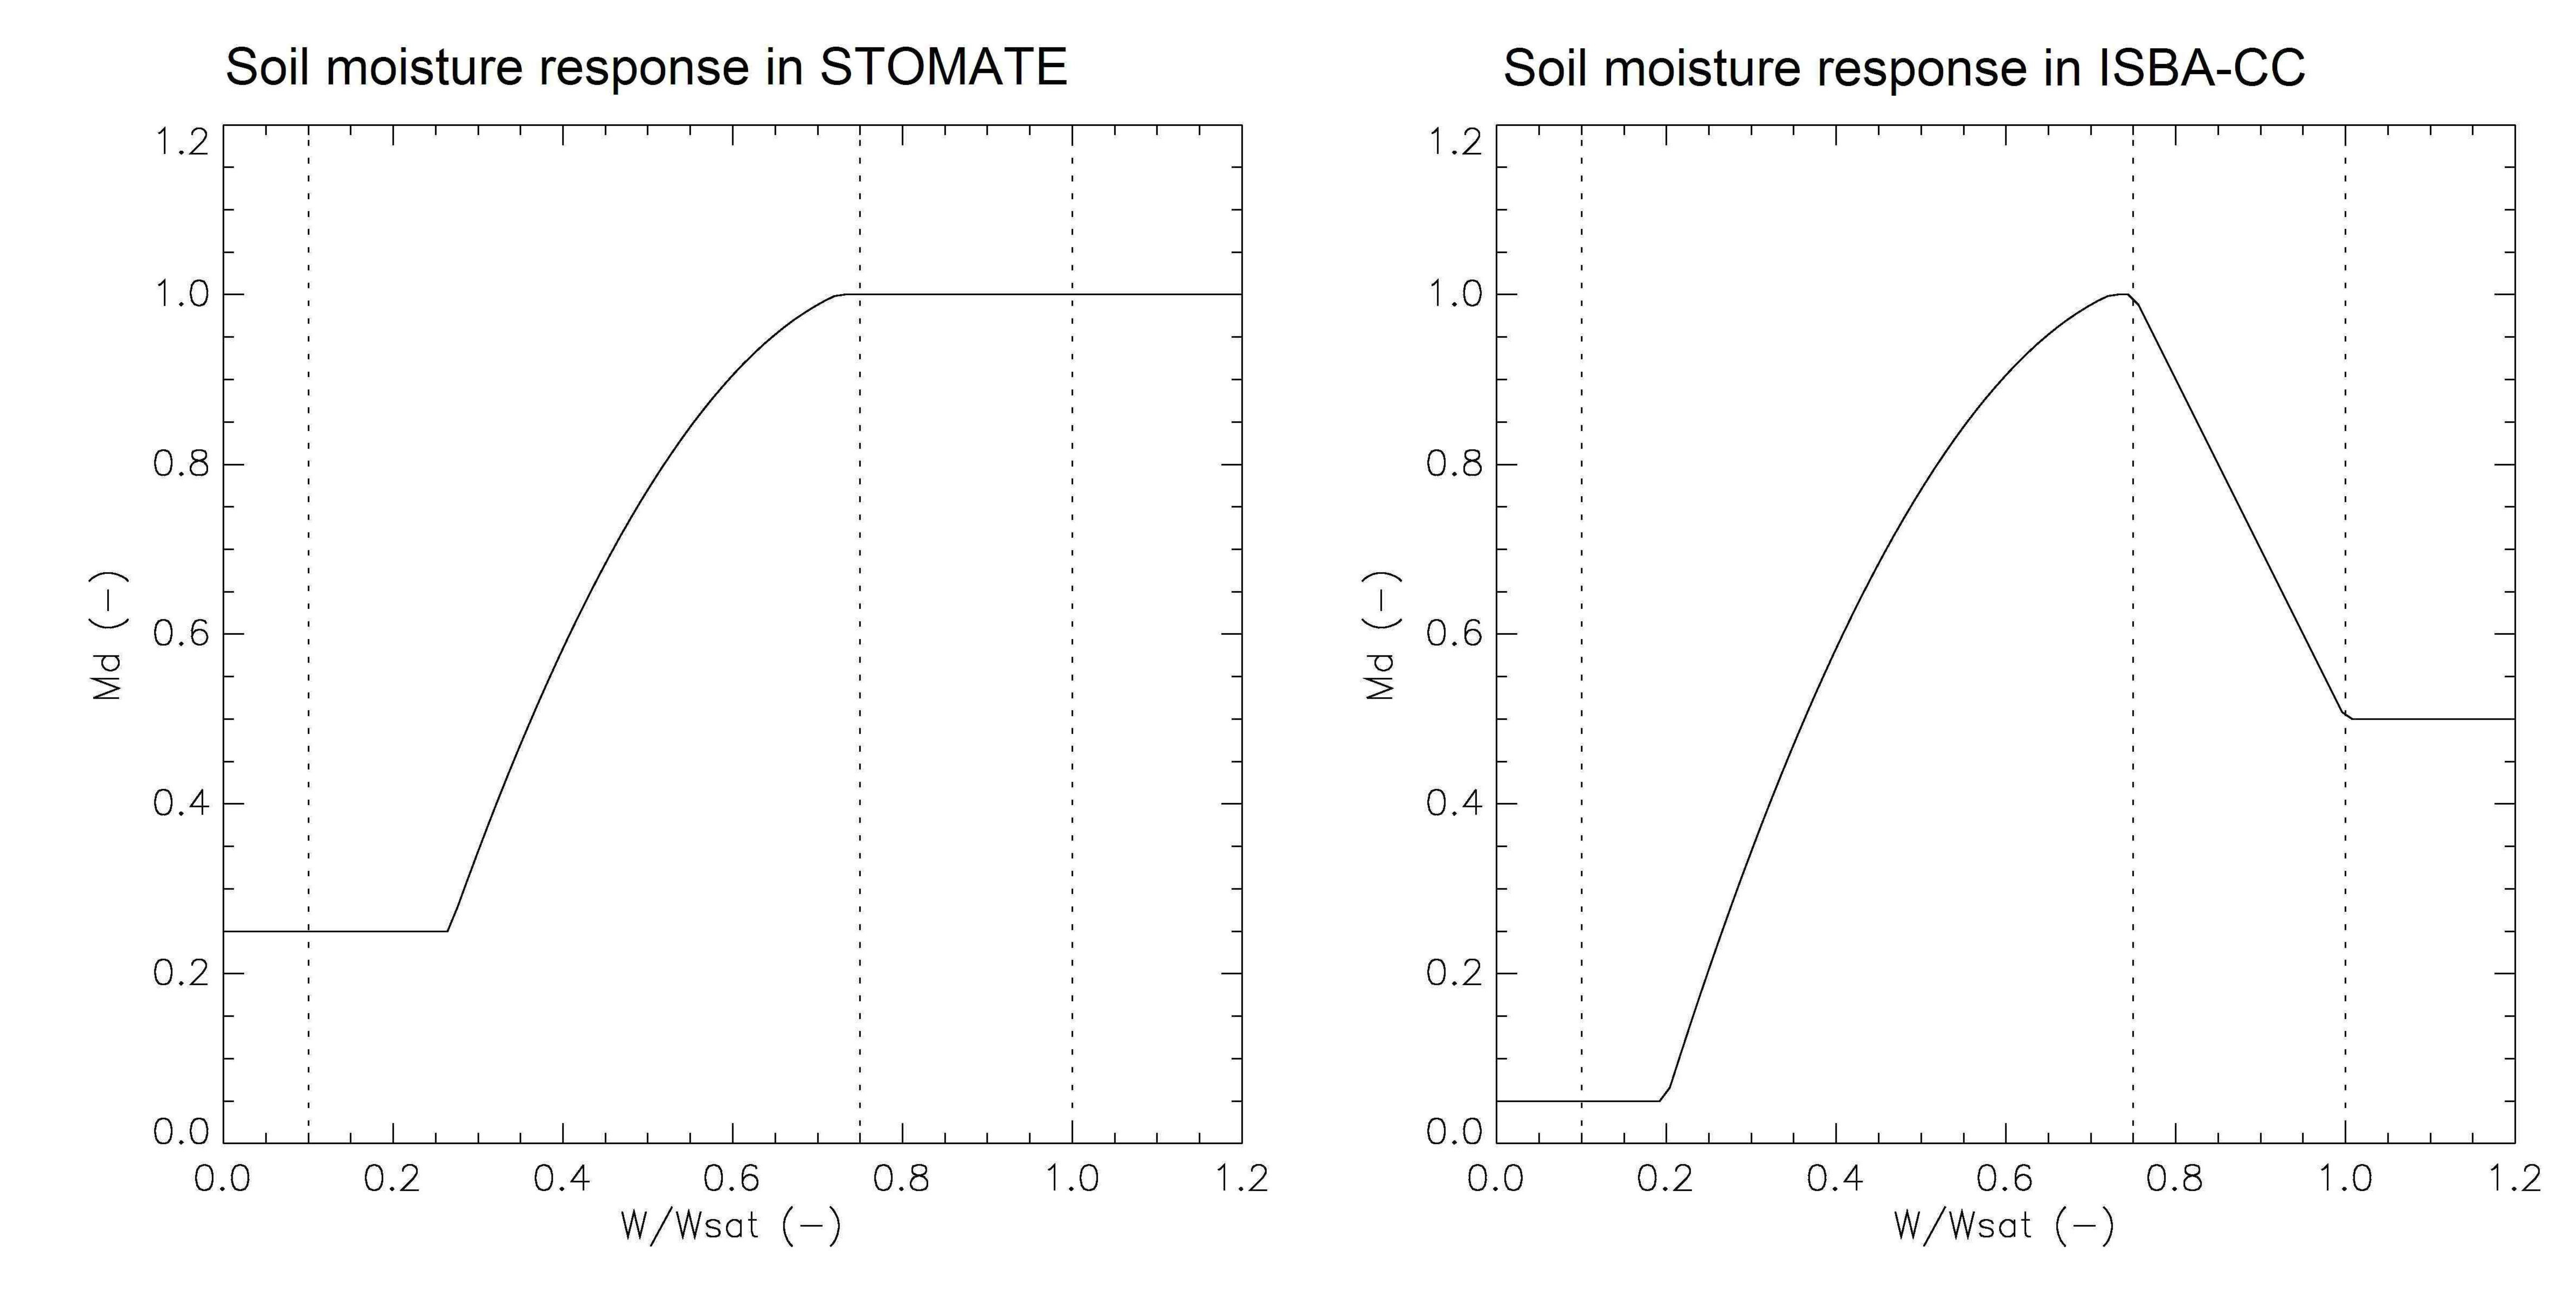
\includegraphics[width=0.9\textwidth]{\EPSDIR/trace_resp_soil_control-soilmoisture.pdf}
\psfig{figure=\EPSDIR/trace_resp_soil_control-soilmoisture.pdf,width=14cm}
\caption{Normalized decomposition response function to soil moisture 
       used in (left) STOMATE-ORCHIDEE and (right) ISBA-CC.
	 The three vertical dashed lines indicate (from left to right) $w_{wilt}$, 
	 $w_{fc}$ and $w_{sat}$.}
\label{fig_moist}
\end{center}
\end{figure}


Since the soil organic matter model does not represent the profile
carbon content of the soil, two soil moisture quantities are used in ISBA-CC: 
the surface soil moisture (a skin soil moisture corresponding to a thin soil layer of about 1cm) 
and the root-zone soil moisture. 
For the litter reservoirs, $w$,
$w_{wilt}$, $w_{fc}$ and $w_{sat}$ correspond to the surface soil moisture.
For the other reservoirs, $w$, $w_{wilt}$, $w_{fc}$ and $w_{sat}$ correspond to the root-zone soil moisture.


In CENTURY, the dependence of the decomposition on temperature is represented by a normalized factor, $T_d$,
driven by the average monthly temperature, according to a bell curve (Parton \etal 1987).

In STOMATE, $T_d$ is defined as:

\begin{equation}
T_d = 2 ^ {(\frac{T-30}{10})}
\end{equation}

where $T$ is soil temperature in units of $^{\circ}$C.
This formulation is used in ISBA-CC, also.

The $T_d$ values used in STOMATE and ISBA-CC are shown by Fig. \ref{fig_temp}.


%\begin{figure}[htb]
%\begin{figure}[htbp]
\begin{figure}[h]
\begin{center}
%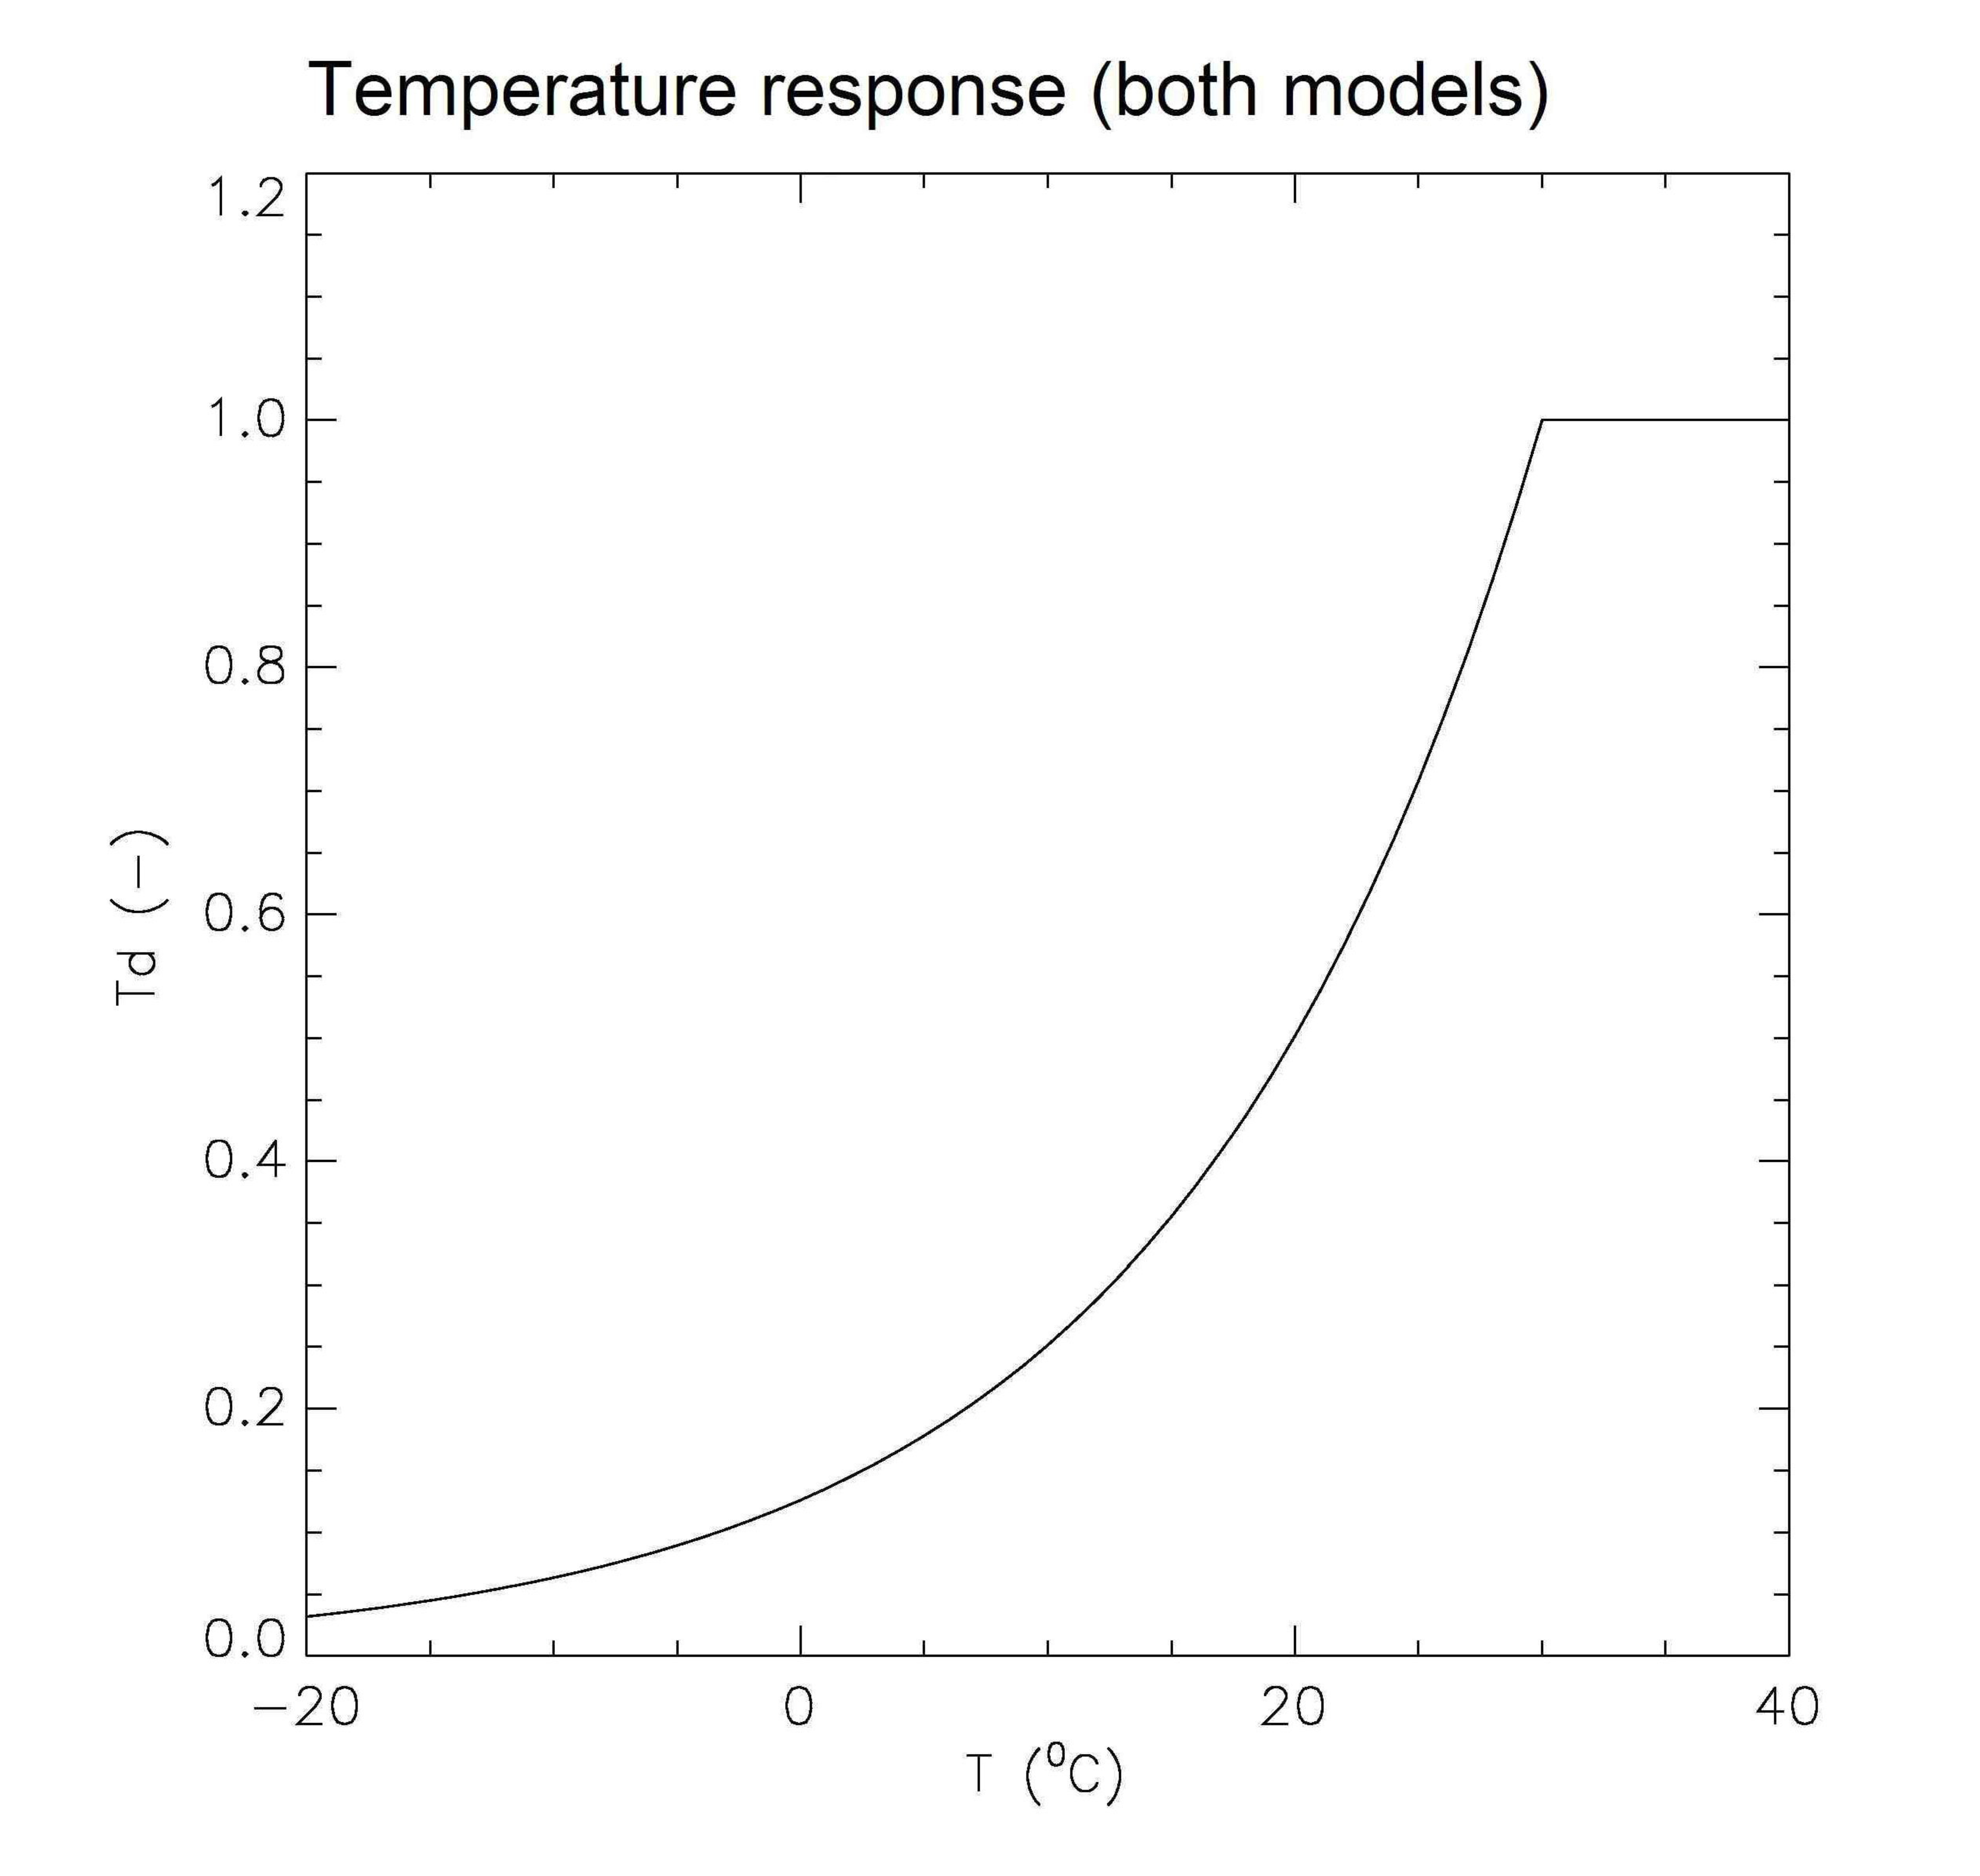
\includegraphics[width=0.9\textwidth]{\EPSDIR/trace_resp_soil_control-temperature.pdf}
\psfig{figure=\EPSDIR/trace_resp_soil_control-temperature.pdf,width=10cm}
\caption{Normalized decomposition response function to soil temperature 
         used in both STOMATE-ORCHIDEE and ISBA-CC.}
\label{fig_temp}
\end{center}
\end{figure}


Since the soil organic matter model does not represent the profile
carbon content of the soil, two soil temperature quantities are used in ISBA-CC: 
the surface temperature $T_s$ 
and a deep soil temperature $T_p$. 
For the litter reservoirs, $T$ = $T_s$.
For the other reservoirs, $T$ = $T_p$.


%=========================================================================================================
\subsubsection{Carbon fluxes}
%=========================================================================================================

The  decomposition of the organic matter contained in the soil carbon reservoir $i$, 
$dC_i/dt$, 
triggers various carbon fluxes (Fig. \ref{fig_soil}).
A fraction of the decomposed organic matter $f_{i,CO_2}$ is mineralized through the respiration process 
and released as CO$_2$ to the atmosphere. 
The other fraction is allocated to the other carbon pools of the soil, based on their 
resistance to decomposition. The fraction of the decomposition flux from reservoir $i$ 
to reservoir $j$ is $f_{i,j}$, and:


\begin{equation}
\sum_j f_{i,j}\ + f_{i,CO_2} = 1
\end{equation}


For the structural litter reservoirs, the decomposition supplies the respiration flux 
and the stabilisation of carbon into a soil organic matter carbon pool, either active or slow, 
depending on the lignin content of the litter and on the nature of the litter (above-ground or below-ground).
The lignin tends to reduce both the mineralization and the decomposition of the plant residues.

For the above-ground structural litter, the fractions are defined as:

\begin{equation}
\begin{tabular}{l}
$ f_{1,5} = 0.55 \: ( 1 - L_1 ) $ \\
$ f_{1,6} = 0.7 \: L_1 $ \\
$ f_{1,CO_2} = 0.45 \: ( 1 - L_1 ) + 0.3 \: L_1 $ \\
\end{tabular}
\end{equation}

where $L_1$ is the lignin fraction of the above-ground structural litter reservoir.

For the below-ground structural litter, the fractions are slightly different, in relation to 
a lower efficiency of the decomposition process to stabilize carbon into the active soil organic matter pool:

\begin{equation}
\begin{tabular}{l}
$ f_{3,5} = 0.45 \: ( 1 - L_3 ) $ \\
$ f_{3,6} = 0.7 \: L_3 $ \\
$ f_{3,CO_2} = 0.55 \: ( 1 - L_3 ) + 0.3 \: L_3 $ \\
\end{tabular}
\end{equation}

where $L_3$ is the lignin fraction of the below-ground structural litter reservoir.

The decomposition of the metabolic litter reservoirs supplies the respiration flux 
and the stabilization of carbon into the active soil organic matter carbon pool. 
The fractions are the same for above-ground and below-ground reservoirs:

\begin{equation}
\begin{tabular}{l}
$ f_{2,5} = 0.45 $ \\
$ f_{2,CO_2} = 0.55 $ \\
\\
$ f_{4,5} = 0.45 $ \\
$ f_{4,CO_2} = 0.55 $ \\
\end{tabular}
\end{equation}

The decomposition of the active soil organic matter carbon pool supplies the respiration flux 
and the slow and passive soil organic matter carbon pools, based on 
soil texture: 

\begin{equation}
\begin{tabular}{l}
$ f_{5,6} = 1 - 0.004 - ( 0.85 - 0.68 \: (f_{silt}+f_{clay}) ) $ \\
$ f_{5,7} = 0.004 $ \\
$ f_{5,CO_2} = 0.85 - 0.68 \: (f_{silt}+f_{clay}) $ \\
\end{tabular}
\end{equation}

The $f_{5,6}$ and $f_{5,CO_2}$ terms are identical to those used in CENTURY.
Note that in STOMATE, $f_{clay}$ is used instead of the $(f_{silt}+f_{clay})$ term. 

The decomposition of the slow soil organic matter carbon pool supplies the respiration flux 
and the active and passive soil organic matter carbon pools, based on soil texture: 

\begin{equation}
\begin{tabular}{l}
$ f_{6,5} = 0.42 $ \\
$ f_{6,7} = 0.03 $ \\
$ f_{6,CO_2} = 0.55 $ \\
\end{tabular}
\end{equation}

Finally, the decomposition of the passive soil organic matter carbon pool supplies the respiration flux 
and the active soil organic matter carbon pool.

\begin{equation}
\begin{tabular}{l}
$ f_{7,5} = 0.45 $ \\
$ f_{7,CO_2} = 0.55 $ \\
\end{tabular}
\end{equation}



%=========================================================================================================
%=========================================================================================================
\subsection{Description of a simulation with ISBA-CC}{Not up-to-date, new version to be released by June 2018}
%=========================================================================================================
%=========================================================================================================

ISBA-CC describes the evolution of several prognostic variables:
the plant biomass reservoirs and the soil organic matter reservoirs.
Prescribing initial or equilibrium values of these reservoirs is not easy, at both 
local and global scales. 
Indeed, accurate observations of these quantities are lacking. 
More often than not, the various biomass components are not measured separately, 
or do not correspond to the definition of the modelled compartments. 
Also, the soil carbon observations are sparse, and generally concern the first top centimeters 
of the soil, rarely below 30cm, and barely ever below 1m.

In order to avoid drifts in the carbon reservoirs, spin-up simulations must be performed, 
until equilibrium reservoir values are reached. 
Whereas the initial CENTURY model was designed to work at a monthly scale, ISBA-CC accounts for 
the diurnal cycle and is coupled with a land surface model working at the half-hourly time scale or better.
As the time scale for reaching equilibrium values is about a few hundred years for wood 
and several thousand years for the passive soil carbon pool, the spin-up simulations concern 
very long periods of time.
Therefore, the spin-up simulations cannot involve the whole coupled model. Instead, the carbon reservoir 
spin-up is performed offline, in several steps described below.

\begin{enumerate}
\item A first spin-up simulation (a few years) is performed with ISBA-CC in order to 
  initialize the soil moisture reservoirs, together with the biomass reservoirs presenting 
  a relatively high turnover such as leaves and the plant structural biomass. 
  For the woody plant types, the wood allocation terms resulting from this simulation are stored
  at a daily time step (see Section \ref{subs:isbacc_alim}).
\item An offline program produces the evolution of wood reservoirs, at a daily time step, 
  until equilibrium has been reached, using the allocation and decline terms. 
  The latter depends on the amount of carbon stored in the reservoir  
  (Section \ref{subs:isbacc_decl}), and as such must be recalculated every day.
\item A second ISBA-CC simulation is performed, in order to calculate and store daily surface and deep 
  soil temperature and soil moisture values. Also, the mortality fluxes of the plant biomass reservoirs 
  are obtained.
\item An offline program produces the evolution of the soil carbon reservoirs, at a monthly time step, 
  until equilibrium has been reached, using the mortality fluxes and the soil temperature and soil moisture values,
  based on the equations listed in Section \ref{sect:isbacc_soil}.
  The equilibrium is reached after several thousand years. It must be noted that since the use 
  of a monthly time step tends to filter out
  the variability of the surface soil moisture, the obtained equilibrium values may 
  differ from those that would have been obtained using a daily time step.
\item Finally, a last ISBA-CC simulation permits the spin-up
  of the litter reservoirs and of the active soil organic matter.
\end{enumerate}

A major shortcoming of this equilibrium method is that on an annual or multi-annual basis, the 
litter supply and the gross primary production are counterbalanced by the heterotrophic respiration, 
and by the autotrophic respiration, respectively.
Therefore, the average net carbon exchange and net primary production present null values.
This method does not permit the determination of long term land carbon sinks and sources. 
Performing more refined carbon budgets at a global scale is very difficult, as a perfect knowledge 
of the initial values of the carbon reservoirs and of the land cover/land use history is needed, 
especially for managed forests and for agricultural lands.
However, the seasonal variability of the carbon fluxes can be represented by this method, as well 
as the impact of extreme events (e.g. droughts).
Also, the equilibrium state can be used to initialize impact simulations related to the response of 
the terrestrial carbon cycle to long term perturbations.

In practise, two SURFEX namelists (NAM\_ISBA and NAM\_PREP\_ISBA\_CARBON) have to be modified before performing ISBA-CC runs.
In NAM\_ISBA, CPHOTO = 'NCB'. In NAM\_PREP\_ISBA\_CARBON, CRESPSL = 'CNT'. The former activates the 6 biomass pools, and the latter activates 
the soil heterotrophic repiration and the soil organic matter pools.
The different steps of spin-up have been coded in a script called spinup\_CC.bsh, 
available on the SURFEX web site. This script automatically perfoms the namelist
changes and the simulation repetitions needed for the spin-up. This script can be
used as a template and be adapted for specifics needs. Please note that the spin-up
procedure is designed for inputs and outputs in ASCII format. In particular, the
NetCDF, and FA formats cannot be used.



%=========================================================================================================
%=========================================================================================================
\subsection{Conclusion}
%=========================================================================================================
%=========================================================================================================

The ISBA-CC model is a new version of ISBA permitting 
the detailed simulation of the land-atmosphere carbon exchange. 
It results from the coupling between ISBA-A-gs (Calvet and Soussana, 2001) 
and the heterotrophic respiration parameterization used in ORCHIDEE (Krinner \etal 2005).
This coupling has required a number of developments.

The ISBA-A-gs allocation scheme was upgraded, in order to simulate all 
the plant biomass compartments, roots and wood in particular (Section \ref{sect:isbacc_biom}).
The principles of the initial allocation scheme, proposed by Calvet and Soussana (2001), were extended 
to the new biomass reservoirs.
All the plant respiration terms are now calculated and their sum represents the autotrophic respiration.
Also, the mortality of the biomass elements is calculated, and supplies the heterotrophic respiration module.
The latter is derived from the parameterization used in ORCHIDEE (Krinner \etal 2005), based on the CENTURY 
model (Parton \etal 1987). It simulates several soil organic matter pools (above-ground and below-ground litter,
and the decomposed organic matter), the carbon fluxes between these pools, and the CO$_2$ flux to the 
atmosphere generated by the heterotrophic respiration (Section \ref{sect:isbacc_soil}).

A few equations differ from the ORCHIDEE parameterization. 
The soil texture effect is based on the original CENTURY formulation, 
i.e. using the silt and clay fraction sum $(f_{silt}+f_{clay})$ 
instead of the mere clay fraction $f_{clay}$ in ORCHIDEE.
Also, the decomposition response to soil moisture is based on 
the saturation soil moisture value $w_{sat}$, available in ISBA simulations. 
This permits the representation of the lower decomposition rates which are observed 
in anaerobic conditions.

The added value of ISBA-CC is the calculation of the two heterotrophic and autotrophic 
respiration terms, allowing the simulation of the net primary production (NPP).
The latter describes the net carbon flux absorbed by the vegetation. 
Also, wood compartments are simulated, and even if forest management processes are not represented so far, 
forest biomass estimates can be used, to some extent, to validate the model simulations.

A complete ISBA-CC simulation has to be made in several steps, including three simulations separated 
by offline spin-up simulations of (1) the plant biomass reservoirs, and (2) the soil carbon pools.

This method produces equilibrium simulations and does not permit the determination 
of long term land carbon sinks and sources. 
However, the seasonal variability of the carbon fluxes can be represented by this method, as well 
as the impact of extreme events (e.g. droughts) and of climate change.


%---------------------------------------------------------------------------



%====================
\bibliography{surfex_scidoc}
%====================
